\chapter{Finite-dimensional vector spaces and linear algebra}
\label{ch:lvs}

\begin{quote}
{\it ``I would have written a shorter letter, but I did not have the time.''}
(Literally: {\it ``I made this [letter] very long because I did not have the leisure to make it shorter.''})
Blaise Pascal, {\it Provincial Letters: Letter XVI (English Translation)}\\
{\it ``Perhaps if I had spent more time I should have been able to make a shorter report~$\ldots$''}
James Clerk Maxwell~\cite[-20mm]{garber}, Document~15,  p.~426
\end{quote}

\newthought{Vector Spaces} are prevalent in physics;
they are essential for an understanding
of mechanics, relativity theory, quantum mechanics, and statistical physics.

\section{Conventions and basic definitions}



This presentation is greatly inspired
by Halmos' compact yet comprehensive treatment
``Finite-Dimensional Vector Spaces''.\cite[-40mm]{halmos-vs}
I greatly encourage the reader to have a look into that book.
Of course, there exist zillions of other very nice presentations, among them
Greub's ``Linear algebra,'' and
Strang's ``Introduction to Linear Algebra,''
among many others, even freely downloadable  ones
\cite[-30mm]{Greub75,Strang:2009:ILA,Homes-rorres,lipschutz:schaul-la,Hefferon}
%Homes and Chris Rorres'  ``Elementary Linear Algebra: Applications Version''\cite{Homes-rorres},
%Mathews' ``Elementary Linear Algebra''\cite{Mathews-LA} (an eprint),
%or Schaum's Outlines\cite{lipschutz:schaul-la}, to name just a very few among the many
competing for your attention.

Unless stated differently, only
finite-dimensional vector spaces will be considered.

In what follows
the overline sign stands for complex conjugation; that is,
if
${a}= \Re a +i\Im a $ is a complex number, then
$\overline{a}= \Re a -i\Im a$.
Very often vector and other coordinates will be real- or complex-valued scalars, which are elements of a field (see Section~\ref{2017-m-ch-fdvs-fields}).

A superscript ``$\intercal$'' means transposition.

The physically oriented notation in Mermin's book on
quantum information theory\cite[-7mm]{mermin-04} is adopted.
Vectors are either typed in boldface, or in Dirac's ``bra-ket'' notation.\cite{dirac}
Both notations will be used simultaneously and equivalently;
not to confuse or obfuscate, but to make  the reader familiar with the bra-ket
notation used in quantum physics.

Thereby,
the vector ${\bf x}$ is identified with the ``ket vector'' $\vert {\bf x}\rangle$.
Ket vectors will be represented by column vectors, that is, by vertically arranged tuples of scalars,
or, equivalently, as $n \times 1$ matrices; that is,
\begin{equation}
{\bf x}
\equiv
\vert {\bf x}\rangle
\equiv
\begin{pmatrix}
x_1\\
x_2\\
\vdots \\
x_n
\end{pmatrix}
=\begin{pmatrix}
x_1,
x_2,
\ldots ,
x_n
\end{pmatrix}^\intercal
.
\end{equation}


A vector ${\bf x}^\ast$ with an asterisk symbol ``$\ast$'' in its superscript denotes an element of the dual space (see later, Section \ref{2011-m-dvs} on page \pageref{2011-m-dvs}).
It is also identified with the ``bra vector'' $\langle {\bf x}\vert$.
\index{ket vector}
\index{bra vector}
Bra vectors will be represented by row vectors, that is, by horizontally arranged tuples of scalars,
or, equivalently, as $1 \times n$ matrices; that is,
\begin{equation}
{\bf x}^\ast
\equiv
\langle {\bf x}   \vert
\equiv
\begin{pmatrix}
x_1,
x_2,
\ldots ,
x_n
\end{pmatrix}
.
\end{equation}



\index{inner product}
\index{scalar product}
Dot (scalar or inner) products between two vectors ${\bf x}$ and ${\bf y}$   in Euclidean space are then
denoted by ``$\langle \textrm{bra} \vert  (\textrm{c}) \vert \textrm{ket}  \rangle$''  form;
that is, by $\langle {\bf x} \vert  {\bf y}  \rangle$.




For an $n \times m$ matrix $\textsf{\textbf{A}}\equiv a_{ij}$ we shall use the following {\em index notation}:
suppose the (column) index $j$  indicates their column number in a matrix-like object $a_{i{\color{red} j}}$ ``runs {\em horizontally},'' that is, from left to right.
The (row) index $i$  indicates their row number in a matrix-like object  $a_{{\color{red}  i}j}$ ``runs {\em vertically},''
so that, with
$1 \le i \le n$ and
$1 \le j \le m$,
\index{index notation}
\begin{equation}
\textsf{\textbf{A}}
\equiv
\begin{pmatrix}
a_{11}&a_{12}& \cdots & a_{1m}\\
a_{21}&a_{22}& \cdots & a_{2m}\\
\vdots &\vdots & \ddots & \vdots \\
a_{n1}&a_{n2}& \cdots & a_{nm}
\end{pmatrix}
\equiv a_{ij}
.
\label{2016-m-ch-fdvs-matrixind}
\end{equation}
Stated differently, $a_{ij}$ is the element  of the table representing $\textsf{\textbf{A}}$ which is in the $i$th row and in the $j$th column.

A {\em matrix multiplication}
\index{matrix multiplication} (written with or without dot)
$\textsf{\textbf{A}} \cdot \textsf{\textbf{B}} = \textsf{\textbf{A}}  \textsf{\textbf{B}}$
of an $n \times m$ matrix $\textsf{\textbf{A}}\equiv a_{ij}$
with an $m \times l$ matrix $\textsf{\textbf{B}}\equiv b_{pq}$
can then be written as an $n \times l$ matrix
$\textsf{\textbf{A}} \cdot \textsf{\textbf{B}} \equiv a_{ij}b_{jk}$,
$1\le i\le n$,
$1\le j\le m$,
$1\le k\le l$.
Here the {\em Einstein summation convention}
\index{Einstein summation convention}
$a_{ij}b_{jk} = \sum_j a_{ij}b_{jk}$
has been used,
which requires that, when an index variable appears twice in a single term, one has to
sum over all of the possible index values.
Stated differently, if $\textsf{\textbf{A}}$ is an $n \times m$ matrix and $\textsf{\textbf{B}}$ is an $m \times l$ matrix,
their matrix product $\textsf{\textbf{A}}\textsf{\textbf{B}}$ is an $n \times l$ matrix, in which the $m$
entries across the rows of $\textsf{\textbf{A}}$ are multiplied with the $m$ entries down the columns of $\textsf{\textbf{B}}$.

As stated earlier ket and bra vectors (from the original or the dual vector space; exact definitions will be given later)
will be encoded -- with respect to a basis or coordinate system -- as an $n$-tuple of numbers;
which are arranged either in $n \times 1$ matrices (column vectors),
or in $1 \times n$ matrices (row vectors), respectively.
We can then write certain terms very compactly (alas often misleadingly).
Suppose, for instance, that
$\vert {\bf x} \rangle \equiv {\bf x}\equiv \begin{pmatrix}x_1, x_2,\ldots ,x_n\end{pmatrix}^\intercal $
and
$\vert {\bf y} \rangle \equiv {\bf y}\equiv \begin{pmatrix}y_1, y_2,\ldots ,y_n\end{pmatrix}^\intercal $
are two (column) vectors (with respect to a given basis).
Then, $x_iy_j a_{ij}$ can (somewhat superficially) be represented as a matrix multiplication ${\bf x}^\intercal  \textsf{\textbf{A}} {\bf y}$ of
a row vector with a matrix and a column vector  yielding a scalar; which in turn can be interpreted as a $1 \times 1$ matrix.
Note that, as ``$\intercal$'' indicates transposition\marginnote{Note that double transposition yields the identity.}
$\left({\bf y}^\intercal \right)^\intercal \equiv \left[ \begin{pmatrix}
y_1,
y_2,
\ldots ,
y_n
\end{pmatrix}^\intercal \right]^\intercal
=
\begin{pmatrix}
y_1,
y_2,
\ldots ,
y_n
\end{pmatrix}
$
represents a row vector, whose components or coordinates with respect to a particular (here undisclosed) basis are the scalars -- that is, an element of a field which will mostly be real or complex numbers -- $y_i$.

\subsection{Fields of real and complex numbers}
\label{2017-m-ch-fdvs-fields}

In physics, scalars occur either as real or complex numbers.
Thus we shall restrict our attention to these cases.

A {\em field}  $\langle  {\Bbb F} , +, \cdot , -, ^{-1}, 0, 1\rangle$
\index{field}
is a set together with two operations,
usually called {\em addition} and {\em multiplication},   denoted by ``$+$'' and ``$\cdot$''
(often  ``$a\cdot b$'' is identified with the expression ``$ab$'' without the center dot)
respectively, such that the following conditions (or, stated differently, axioms) hold:
\begin{itemize}
\item[(i)]
{\bf closure} of ${\Bbb F}$ with respect to addition and multiplication:
for all $a, b \in {\Bbb F}$, both $a + b$ as well as $a   b$ are in ${\Bbb F}$;
\item[(ii)]
{\bf associativity} of addition and multiplication:
for all $a$, $b$, and $c$ in ${\Bbb F}$,
the following equalities hold: $a + (b + c) = (a + b) + c$,
and
$a (b c) = (a  b) c$;
\item[(iii)]
{\bf commutativity} of addition and multiplication:
for all $a$ and $b$ in ${\Bbb F}$, the following equalities hold: $a + b = b + a$ and $a b = b  a$;
\item[(iv)]
additive and multiplicative {\bf identities}:
there exists an element of ${\Bbb F}$,
called the additive identity element and denoted by $0$, such that for all $a$ in ${\Bbb F}$,
$a + 0 = a$.
Likewise, there is an element, called the multiplicative identity element and denoted by $1$,
such that for all $a$ in ${\Bbb F}$, $1 \cdot a  = a$.
(To exclude the trivial ring, the additive identity and the multiplicative
identity are required to be distinct.)
\item[(v)]
additive and multiplicative {\bf inverses}:
for every $a$ in ${\Bbb F}$, there exists an element $-a$ in ${\Bbb F}$, such that $a + (-a) = 0$.
Similarly, for any $a$ in ${\Bbb F}$ other than $0$, there exists an element $a^{-1}$ in ${\Bbb F}$,
such that $a \cdot a^{-1} = 1$.
(The elements $+ (-a)$ and  $a^{-1}$
are also denoted $-a$ and $\frac{1}{a}$, respectively.)
Stated differently: subtraction and division operations exist.
\item[(vi)]
{\bf Distributivity} of multiplication over addition:
For all $a$, $b$ and $c$ in ${\Bbb F}$, the following equality holds:
$a (b + c) = (a  b) + (a  c)$.
\end{itemize}

\subsection{Vectors and vector space}
\marginnote[-7mm]{For proofs and additional information see  {\S}2   in~\bibentry{halmos-vs}.}

Vector spaces are structures or sets  allowing the
summation (addition,  ``coherent superposition'') of objects called ``vectors,'' and the multiplication
of these objects by scalars --  thereby remaining in these structures or sets, and hence satisfying a closure property.
\index{closure}
That is, for instance, the ``coherent superposition''  ${\bf a} + {\bf b}\equiv \vert {\bf a} + {\bf b} \rangle $
\index{coherent superposition}
\index{superposition}
of two vectors ${\bf a} \equiv \vert {\bf a} \rangle $ and ${\bf b} \equiv \vert {\bf b} \rangle $ can be guaranteed to
be a vector.
\sidenote{In order to define {\em length}, we have to engage an additional structure, namely the {\em norm}
$\|  {\bf a} \|$ of a vector ${\bf a}$.
\index{length}
And in order to define relative {\em direction} and {\em orientation}, and, in particular,
{\em orthogonality} and {\em collinearity} we have to define the {\em scalar product}
$\langle {\bf a} \vert {\bf b} \rangle$ of two vectors ${\bf a}$ and ${\bf b}$.
\index{direction}
\index{scalar product}
}
At this stage, little can be said about the length or relative direction or orientation of these ``vectors.''
Algebraically, ``vectors'' are elements of vector spaces.
Geometrically a vector may be interpreted as ``a quantity which is usefully represented by an arrow''.\cite{Weinreich}



A {\em linear vector space}      $\langle  \frak V , +, \cdot , -,  0, 1\rangle$
\index{linear vector space}
is a set $\frak V$ of elements called {\em vectors},
\index{vector}
here denoted by  bold face  symbols such as
$
{\bf a},
{\bf x},
{\bf v},
{\bf w},
\ldots
$,
or, equivalently, denoted by
$
\vert {\bf a}\rangle,
\vert {\bf x}\rangle,
\vert {\bf v}\rangle,
\vert {\bf w}\rangle,
\ldots
$,
satisfying certain conditions (or, stated differently, axioms); among them,
with respect to addition of vectors:
\begin{itemize}
\item[(i)]
{\bf commutativity}, that is, $\vert {\bf x}\rangle + \vert {\bf y}\rangle   = \vert {\bf y}\rangle + \vert {\bf x}\rangle$;
\item[(ii)]
{\bf associativity}, that is, $(\vert {\bf x}\rangle + \vert {\bf y}\rangle ) +  \vert {\bf z}\rangle = \vert {\bf x}\rangle + (\vert {\bf y}\rangle +  \vert {\bf z}\rangle )$;
\item[(iii)]
the uniqueness of the origin or {\bf null vector} $0$;
as well as
\item[(iv)]
the uniqueness of  the {\bf negative vector};
\item[ ]
with respect to multiplication of vectors with scalars:
\item[(v)]
the existence of an {\bf identity} or unit factor $1$; and
\item[(vi)]
{\bf distributivity} with respect to scalar and vector additions; that is,
\begin{equation}
\begin{split}
(\alpha +\beta ){\bf x} = \alpha {\bf x}+\beta  {\bf x}, \\
\alpha ({\bf x} +{\bf y}) = \alpha {\bf x}+\alpha {\bf y},
\end{split}
\end{equation}
with ${\bf x}, {\bf y} \in \frak V$ and scalars $\alpha ,\beta \in  {\Bbb F}$,
respectively.
\end{itemize}

{
\color{blue}
\bexample
Examples of vector spaces are:
\begin{itemize}
\item[(i)]
The set ${\Bbb C}$ of complex numbers: ${\Bbb C}$  can be interpreted as a complex vector space by  interpreting as vector addition and scalar multiplication
as the usual addition and multiplication of complex numbers, and with $0$ as the null vector;
\item[(ii)]
The set ${\Bbb C}^n$, $n \in {\Bbb N}$ of $n$-tuples of complex numbers:
Let
${\bf x}=
(x_1,\ldots , x_n)$
and
${\bf y}=
(y_1,\ldots , y_n)$.
 ${\Bbb C}^n$  can be interpreted as a complex vector space by  interpreting
the ordinary addition  $ {\bf x} + {\bf y} =  (x_1+y_1,\ldots , x_n+y_n)$
and the multiplication $\alpha {\bf x}=
(\alpha  x_1,\ldots ,\alpha  x_n)$ by a complex number $\alpha$ as vector addition
 and scalar multiplication, respectively;
the null tuple $0 =
(0,\ldots ,0)$ is the neutral element of vector addition;
\item[(iii)]
The set ${\frak P}$
 of all polynomials with complex coefficients in a variable~$t$:
${\frak P}$  can be interpreted as a complex vector space by  interpreting
the ordinary addition of polynomials and the multiplication of a polynomial by a complex number as vector addition and scalar multiplication,
respectively;
the null polynomial is the neutral element of vector addition.
\end{itemize}
\eexample
}


\section{Linear independence}

A set ${\frak S}=\{
{\bf x}_1,
{\bf x}_2,
\ldots ,
{\bf x}_k\} \subset {\frak V}$
of vectors ${\bf x}_i$ in a linear vector space
is {\em linearly independent}
\index{linear independence}
if ${\bf x}_i\neq 0\,\forall 1\le i\le k$,
and additionally, if either $k=1$,
or if no vector in ${\frak S}$ can be written as a linear combination of other vectors in this set ${\frak S}$;
that is, there are no scalars $\alpha_j$ satisfying
 ${\bf x}_i=\sum_{1\le j \le k, \; j\neq i}\alpha_j {\bf x}_j$.

Equivalently, if $\sum_{i=1}^k \alpha_i {\bf x}_i = 0$
 implies $\alpha_i =0$ for each $i$, then the set
${\frak S}=\{
{\bf x}_1,
{\bf x}_2,
\ldots ,
{\bf x}_k\}  $ is linearly independent.


Note that the vectors of a basis are linear independent and ``maximal''
insofar as any inclusion of an additional vector results in a linearly dependent set;
that is, this additional vector can be expressed in terms of a linear combination of the
existing basis vectors; see also Section~\ref{2012-m-ch-fdvs-Basis} on page \pageref{2012-m-ch-fdvs-Basis}.

\section{Subspace}
\label{2011-m-subspace}
\marginnote{For proofs and additional information see {\S}10 in~\bibentry{halmos-vs}.}
A nonempty subset ${\frak M}$ of a vector space is a {\em subspace}
\index{subspace}
or, used synonymously,
a {\em linear manifold}\index{linear manifold},
 if, along with every pair of vectors ${\bf x}$   and  ${\bf y}$
 contained in  ${\frak M}$,
 every linear combination
$\alpha {\bf x} + \beta {\bf y}$ is also contained in  ${\frak M}$.

If
${\frak U}$
and
${\frak V}$
are two subspaces of a vector space,
then
${\frak U}+{\frak V}$
is the subspace spanned by
${\frak U}$
and
${\frak V}$;
that is,
it contains all vectors
${\bf z}={\bf x}+{\bf y}$, with
${\bf x}\in {\frak U}$  and
${\bf y}\in {\frak V}$.

${\frak M}$ is the {\em linear span}
\index{linear span}
\index{span}
\begin{equation}
{\frak M}
= \textrm{span}({\frak U},{\frak V})
= \textrm{span}({\bf x},{\bf y}) =
\{\alpha {\bf x} +\beta {\bf y}\mid \alpha ,\beta \in {\Bbb F}, {\bf x} \in {\frak U},
{\bf y} \in {\frak V}\}.
\end{equation}


A generalization to more than two vectors and more than two subspaces is straightforward.


For every vector space ${\frak V}$, the vector space containing only the null vector,
 and the vector space ${\frak V}$ itself are subspaces of ${\frak V}$.

\subsection{Scalar or inner product}
\marginnote{For proofs and additional information see {\S}61 in~\bibentry{halmos-vs}.}
\index{scalar product}
\index{inner product}
\label{2011-m-scalarproduct}

A {\em scalar} or {\em inner} product presents some form of measure of ``distance'' or ``apartness''
of two vectors in a linear vector space.
It should not be confused with the bilinear functionals (introduced on page \pageref{2011-m-dvs}) that connect a vector space with its dual vector space,
although for real Euclidean vector spaces these may coincide,
and although the scalar product is also bilinear in its arguments.
It should also not be confused with the tensor product introduced in Section~\ref{2011-m-tensorp} on page \pageref{2011-m-tensorp}.

An inner product space is a vector space $\frak V$,
together with an inner product; that is, with a map
 $\langle \cdot \vert \cdot \rangle :  \frak V  \times  \frak V  \longrightarrow {\Bbb F}$
 (usually ${\Bbb F}={\Bbb C}$ or ${\Bbb F}={\Bbb R}$)
 that satisfies the following three conditions (or, stated differently, axioms) for all vectors  and all scalars:
\begin{itemize}
\item[(i)]
{\bf Conjugate (Hermitian) symmetry}:
\index{conjugate symmetry}
\index{Hermitian symmetry}
$
\langle {\bf x}\vert {\bf y}\rangle
=
\overline{\langle {\bf y}\vert {\bf x}\rangle }$;
\marginnote{For real, Euclidean vector spaces, this function is symmetric; that is
$
\langle {\bf x}\vert {\bf y}\rangle
=
{\langle {\bf y}\vert {\bf x}\rangle}$.
}
\item[(ii)]
{\bf linearity} in the second argument:
\marginnote{This definition and nomenclature is different from Halmos' axiom which defines linearity in the  {\em first} argument.
We chose linearity in the second argument because this is usually assumed in physics textbooks, and because Thomas Sommer strongly insisted.}
$$
\langle {\bf z}  \vert \alpha{\bf x} + \beta {\bf y} \rangle
=
\alpha {\langle {\bf z}\vert {\bf x}\rangle}
+
\beta {\langle {\bf z}\vert {\bf y}\rangle}
;
$$
\item[(iii)]
\label{2016-m-ch-fdvs-pd}
{\bf positive-definiteness}:
$
\langle {\bf x}\vert {\bf x}\rangle
\ge
0$;  with equality if and only if ${\bf x} = 0$.
\end{itemize}

Note that from the first two properties, it follows that the inner product is
{\em antilinear}, or synonymously,
{\em conjugate-linear}, in its {\em first} argument (note that $\overline{(uv)}= (\overline{u}) {\;} (\overline{v}) $ for all $u,v\in {\Bbb C}$):
\begin{equation}
\begin{split}
 \langle \alpha {\bf x} + \beta {\bf y}   \vert {\bf z}\rangle
 =
 \overline{\langle   {\bf z} \vert \alpha {\bf x} + \beta {\bf y}\rangle }
 =
 \overline{ \alpha}\overline{\langle {\bf z} \vert {\bf x} \rangle}
 + \overline{\beta }\overline{\langle {\bf z} \vert {\bf y} \rangle}
 =
 \overline{\alpha} {\langle {\bf x}\vert {\bf z}\rangle}
 +\overline{\beta} {\langle {\bf y}\vert {\bf z}\rangle}
.
\end{split}
\end{equation}



{
\color{blue}
\bexample
One example of an inner product is  the
{\em dot product}
\index{dot product}
\begin{equation}
\langle {{\bf x}} \vert  {\bf y} \rangle
=
\sum_{i=1}^n \overline{x_i}y_i
\end{equation}
of two vectors ${\bf x}=
(x_1,\ldots , x_n)$
and
${\bf y}=
(y_1,\ldots , y_n)$ in ${\Bbb C}^n$,
which, for real Euclidean space,  reduces to the well-known dot product
$\langle  {\bf x} \vert {\bf y} \rangle
=
{x_1}y_1 + \cdots + {x_n}y_n  = \| {\bf x}\| \| {\bf y}\| \cos \angle ({\bf x},{\bf y})$.


It is mentioned without proof that the most general form of an inner product in ${\Bbb C}^n$
is
$\langle  {\bf x} \vert {\bf y} \rangle
=  {\bf y}^\dagger \textsf{\textbf{A}} {\bf x}= \overline{ {\bf x}^\dagger \textsf{\textbf{A}} {\bf y}}$,
where the symbol ``$\dagger$'' stands for the {\em conjugate transpose} (also denoted as
{\em Hermitian conjugate} or {\em Hermitian adjoint}),
\index{conjugate transpose}
\index{Hermitian conjugate}
\index{Hermitian adjoint}
and $ \textsf{\textbf{A}} $ is a positive definite Hermitian matrix (all of its eigenvalues are positive).
\eexample
}



The {\em norm} of a vector ${\bf x}$
\index{norm}
is defined by
\begin{equation}
\|
{\bf x}
\|
=\sqrt{\langle {\bf x}\vert {\bf x}\rangle }
.
\label{2018-mm-ch-vn}
\end{equation}

Conversely, the {\em polarization identity}
\index{polarization identity}
expresses the inner product of two vectors in terms of the norm of their differences; that is,

\begin{equation}
\langle {\bf x}\vert {\bf y}\rangle
=
\frac{1}{4}\left[
\|  {\bf x}+ {\bf y} \|^2
-
\|  {\bf x}- {\bf y} \|^2
+ i
\left(
 \|  {\bf x}- i{\bf y} \|^2
-
\|  {\bf x}+ i{\bf y} \|^2
\right)
\right]
.
\label{2015-m-ch-polidc}
\end{equation}


{\color{OliveGreen}
\bproof
In complex vector space,  a direct but tedious calculation
-- with conjugate-linearity (antilinearity)
in the first argument and linearity in the second argument of the inner product -- yields
\begin{equation}
\begin{split}
\frac{1}{4}\left(
\|  {\bf x}+ {\bf y} \|^2
-
\|  {\bf x}- {\bf y} \|^2
+ i
\|  {\bf x}- i{\bf y} \|^2
- i
\|  {\bf x}+ i{\bf y} \|^2
\right)
\\
=
\frac{1}{4}\left(
\langle {\bf x}+ {\bf y} \vert {\bf x}+ {\bf y}\rangle
-
\langle {\bf x}- {\bf y} \vert {\bf x}- {\bf y}\rangle
+ i
 \langle {\bf x}- i{\bf y} \vert {\bf x} -i {\bf y}\rangle
- i   \langle {\bf x}+ i{\bf y} \vert {\bf x}+ i{\bf y}\rangle
\right)
\\
=
\frac{1}{4}\left[
(
\langle {\bf x} \vert {\bf x}\rangle +
\langle {\bf x} \vert {\bf y}\rangle +
\langle {\bf y} \vert  {\bf x}\rangle +
\langle {\bf y} \vert {\bf y}\rangle
)
-
(
 \langle {\bf x} \vert {\bf x}\rangle    -
\langle {\bf x} \vert {\bf y}\rangle    -
\langle {\bf y} \vert {\bf x}\rangle    +
\langle {\bf y} \vert {\bf y}\rangle
)
\right.
\\
\left.
+ i
(
\langle {\bf x} \vert {\bf x}\rangle -
\langle {\bf x} \vert i {\bf y}\rangle  -
\langle i{\bf y} \vert {\bf x}\rangle  +
\langle  i{\bf y} \vert i {\bf y}\rangle
)
- i
(
\langle {\bf x} \vert {\bf x}\rangle +
\langle {\bf x} \vert  i{\bf y}\rangle  +
\langle i{\bf y} \vert {\bf x}\rangle   +
\langle i{\bf y} \vert i{\bf y}\rangle
)
\right]
\\
=
\frac{1}{4}\left[
\langle {\bf x} \vert {\bf x}\rangle +
\langle {\bf x} \vert {\bf y}\rangle +
\langle {\bf y} \vert  {\bf x}\rangle +
\langle {\bf y} \vert {\bf y}\rangle
-
\langle {\bf x} \vert {\bf x}\rangle    +
\langle {\bf x} \vert {\bf y}\rangle    +
\langle {\bf y} \vert {\bf x}\rangle    -
\langle {\bf y} \vert {\bf y}\rangle
)
\right.
\\
\left.
+
i \langle {\bf x} \vert {\bf x}\rangle -
i\langle {\bf x} \vert  i{\bf y}\rangle  -
i\langle i{\bf y} \vert {\bf x}\rangle   +
i\langle i{\bf y} \vert i{\bf y}\rangle
-
i\langle {\bf x} \vert {\bf x}\rangle -
i\langle {\bf x} \vert i {\bf y}\rangle -
i\langle i{\bf y} \vert {\bf x}\rangle  -
i\langle  i{\bf y} \vert i {\bf y}\rangle
)
\right]
\\
=
\frac{1}{4}\left[
2 (
\langle {\bf x} \vert {\bf y}\rangle +
\langle {\bf y} \vert  {\bf x}\rangle
)
- 2 i (
\langle {\bf x} \vert  i{\bf y}\rangle  +
\langle i{\bf y} \vert {\bf x}\rangle
)
\right]
\\
=
\frac{1}{2}\left[
(
\langle {\bf x} \vert {\bf y}\rangle +
\langle {\bf y} \vert  {\bf x}\rangle
)
- i (
i\langle {\bf x} \vert  {\bf y}\rangle     -
i\langle {\bf y} \vert {\bf x}\rangle
)
\right]
\\
=
\frac{1}{2}\left[
\langle {\bf x} \vert {\bf y}\rangle +
\langle {\bf y} \vert  {\bf x}\rangle
+
\langle {\bf x} \vert  {\bf y}\rangle
-\langle {\bf y} \vert {\bf x}\rangle
\right]
=
\langle {\bf x} \vert {\bf y}\rangle
.
\end{split}
\label{2015-m-ch-polidc2}
\end{equation}
\eproof
}


For any real vector space the imaginary terms in (\ref{2015-m-ch-polidc}) are absent, and (\ref{2015-m-ch-polidc}) reduces to
\begin{equation}
\langle {\bf x}\vert {\bf y}\rangle
=
\frac{1}{4}\left(
\langle {\bf x}+ {\bf y} \vert {\bf x}+ {\bf y}\rangle
-
\langle {\bf x}- {\bf y} \vert {\bf x}- {\bf y}\rangle
\right)
=
\frac{1}{4}\left(
\|  {\bf x}+ {\bf y} \|^2
-
\|  {\bf x}- {\bf y} \|^2
\right).
\label{2015-m-ch-polidr}
\end{equation}


Two nonzero vectors $  {\bf x} , {\bf y} \in {\frak V}$,  $  {\bf x},   {\bf y}\neq 0$
are {\em orthogonal}, denoted by ``${\bf x} \perp {\bf y}$''
\index{othogonality}
if their scalar product vanishes; that is, if
\begin{equation}
\langle  {\bf x} \vert {\bf y} \rangle   = 0.
\end{equation}


Let ${\frak E}$ be any set of vectors in an inner product space ${\frak V}$.
The symbol
\begin{equation}
{\frak E}^\perp  = \left\{ {\bf x}\mid  \langle  {\bf x} \vert {\bf y} \rangle=0,  {\bf x} \in {\frak V},
\forall {\bf y} \in {\frak E} \right\}
\end{equation}
 denotes the set of all vectors in  ${\frak V}$ that are
orthogonal to every vector in  ${\frak E}$.

Note that, regardless of whether or not ${\frak E}$ is a subspace,
\marginnote{See page \pageref {2011-m-subspace} for a definition of subspace.}
${\frak E}^\perp$ is a subspace.
Furthermore,
${\frak E}$  is contained in $({\frak E}^\perp)^\perp= {\frak E}^{\perp\perp}$.
In case ${\frak E}$ is a subspace, we call ${\frak E}^\perp$
the {\em orthogonal complement}
\index{orthogonal complement}
of ${\frak E}$.

The following {\em projection theorem}
\index{projection theorem}
is mentioned without proof.
If ${\frak M}$ is any subspace of a finite-dimensional inner product space ${\frak V}$,
then ${\frak V}$ is the direct sum of ${\frak M}$ and ${\frak M}^\perp$;
that is, ${\frak M}^{\perp \perp}={\frak M}$.

{
\color{blue}
\bexample
For the sake of an example, suppose ${\frak V}={\Bbb R}^2$,
and take ${\frak E}$ to be the set of all vectors spanned by the vector $(1,0)$;
then ${\frak E}^\perp$ is the set of all vectors spanned by $(0,1)$.
\eexample
}


\subsection{Hilbert space}


A (quantum mechanical) {\em Hilbert space}  is a linear
\index{Hilbert space}
vector space ${\frak V}$ over the field ${\Bbb C}$ of complex numbers
(sometimes only ${\Bbb R}$ is used)
equipped with vector addition, scalar multiplication, and some inner (scalar) product.
Furthermore, {\em completeness}
by the Cauchy criterion for sequences
is an additional requirement,
but nobody has made operational sense of that so far:
If ${\bf x}_n\in {\frak V}$, $n=1,2,\ldots$, and if $\lim_{n,m\rightarrow
\infty} ({\bf x}_n-{\bf x}_m,{\bf x}_n-{\bf x}_m)=0$,
then there exists an ${\bf x}\in {\frak V}$ with
$\lim_{n\rightarrow \infty} ({\bf x}_n-{\bf x},{\bf x}_n-{\bf x})=0$.





Infinite dimensional vector spaces and continuous spectra are nontrivial
extensions of the finite
dimensional Hilbert space treatment. As a heuristic rule -- which is not
always correct -- it might be
stated that the sums become integrals, and the Kronecker delta function
$\delta_{ij}$ defined by
\index{Kronecker delta function}
\begin{equation}
\delta_{ij} =\begin{cases}
0  &\text{ for }i\neq j , \\
1  &\text{ for }i = j.
\end{cases}
\end{equation}
becomes the Dirac delta function $\delta (x-y)$, which is a
generalized function in the continuous variables $x,y$.
In the Dirac bra-ket notation, the resolution of the identity operator,
sometimes also referred to as {\em completeness}, is given by
\index{resolution of the identity}
\index{completeness}
$\mathbb{1} = \int_{-\infty}^{+\infty} \vert x\rangle \langle  x\vert \, dx$.
For a careful treatment, see, for instance,
the books by
Reed and Simon,\cite{reed-sim1,reed-sim2}
or wait for Chapter~\ref{2011-m-ch:gf}, page~\pageref{2011-m-ch:gf}.


\section{Basis}
\label{2012-m-ch-fdvs-Basis}
\marginnote{For proofs and additional information see {\S}7 in~\bibentry{halmos-vs}.}

We shall use bases of vector spaces to formally represent vectors (elements) therein.

A (linear) {\em basis}
\index{basis}
[or a {\em coordinate system}, or a {\em frame (of reference)}]
\index{coordinate system}
\index{frame}
is a set    $\frak B$
of linearly independent vectors
such that every vector
in $\frak V$ is a linear combination of the vectors in the basis; hence
$\frak B$ spans $\frak V$.

What particular basis should one choose?
{\em A priori} no basis is privileged over the other.
Yet, in view of certain (mutual) properties of elements of some bases (such as orthogonality or orthonormality)
we shall prefer some or one over others.


Note that a vector is some directed entity with a particular length,
oriented in some (vector) ``space.''
It is ``laid out there'' in front of our eyes, as it is: some directed entity.
{\it A priori}, this space, in its most primitive form,
is not equipped with a basis, or synonymously, a frame of reference, or reference frame.
Insofar it is not yet coordinatized.
In order to formalize the notion of a vector, we have to encode this vector by ``coordinates''
or ``components'' which are the coefficients with respect to a (de)composition into basis elements.
Therefore, just as for numbers (e.g., by different numeral bases, or by prime decomposition),
there exist many ``competing'' ways to encode a vector.

Some of these ways appear to be rather straightforward,
such as, in particular, the {\em Cartesian basis},
also synonymously called the  {\em standard basis}.
\index{Cartesian basis}
\index{standard basis}
It is, however, not in any way {\it a priori}
``evident'' or ``necessary'' what should be specified to be ``the Cartesian basis.''
Actually, specification of a ``Cartesian basis'' seems to be mainly motivated by
physical inertial motion --
and thus identified with some inertial frame of reference --
``without any friction and
forces,'' resulting in a ``straight line motion at constant speed.''
(This sentence is  cyclic because heuristically any such absence of ``friction and
force''  can only be operationalized by testing if the motion is a
``straight line motion at constant speed.'')
If we grant that in this way straight lines can be defined, then
Cartesian bases in Euclidean vector spaces can be characterized by
orthogonal (orthogonality is defined {\it via} vanishing scalar products between nonzero vectors)
straight lines spanning the entire space.
In this way, we arrive, say for a planar situation, at the coordinates
characterized by some basis $\{(0,1),(1,0)\}$,
where, for instance, the basis vector ``$(1,0)$'' literally and physically
means ``a unit arrow pointing in some particular, specified direction.''

Alas, if we would prefer, say, cyclic motion in the plane,
we might want to call a frame based on the polar coordinates $r$ and $\theta$ ``Cartesian,''
resulting in some ``Cartesian basis'' $\{(0,1),(1,0)\}$;
but this ``Cartesian basis'' would be very different from the Cartesian
basis mentioned earlier,
as ``$(1,0)$'' would refer to some specific unit radius,
and ``$(0,1)$'' would refer to some specific unit angle (with respect to a specific zero angle).
In terms of the ``straight'' coordinates (with respect to ``the usual Cartesian basis'')
$x,y$, the polar coordinates are $r = \sqrt{x^2+y^2}$ and $\theta = \mathrm{tan}^{-1} (y/x)$.
We obtain the original ``straight'' coordinates (with respect to ``the usual Cartesian basis'')
back if we take
$x=r\cos \theta$
and
$y=r\sin \theta$.

Other bases than the ``Cartesian'' one may be less suggestive at first; alas it may be ``economical'' or pragmatical to use them;
mostly to cope with, and adapt to, the {\em symmetry} of a physical configuration:
if the physical situation at hand is, for instance, rotationally invariant,
we might want to use rotationally invariant bases --
such as, for instance, polar coordinates in two dimensions, or spherical coordinates in three dimensions --
to represent a vector, or, more generally, to encode any given representation of a physical entity
(e.g., tensors, operators) by such bases.


\section{Dimension}
\marginnote{For proofs and additional information see {\S}8 in~\bibentry{halmos-vs}.}
The {\em dimension}
\index{dimension}
of $\frak V$ is the number of elements in $\frak B$.

All bases $\frak B$ of $\frak V$ contain the same number of elements.

A vector space is finite dimensional if its bases are finite; that is, its bases
contain a finite number of elements.

{\color{Purple}
In quantum physics, the dimension of a quantized system is associated with
the {\em number of mutually exclusive measurement outcomes}.
For a spin state measurement of an electron
along with a particular direction,
as well as for a measurement of the linear polarization
of a photon in a particular direction,
the dimension is two, since both measurements
may yield two distinct outcomes
which we can
interpret as vectors in two-dimensional Hilbert space,
which, in Dirac's bra-ket notation,\cite{dirac} can be written as
$
\vert \uparrow \rangle$ and $\vert \downarrow \rangle$,
or $\vert + \rangle$ and $
\vert - \rangle
$,
or
$
\vert H \rangle $ and $
\vert V \rangle
$,
or
$
\vert 0 \rangle $ and $
\vert 1 \rangle
$,
or
$
\bigg|$\raisebox{-0.4\height}{
\begin{tikzpicture}
    \emoticon\pupils
    %% mouth
    \draw[very thick,red,line cap=round] (-1ex,-1ex)
               ..controls (-0.5ex,-1.5ex)and(0.5ex,-1.5ex)..(1ex,-1ex);
    %% eyelashes
    \draw (0.60ex,1.20ex)--(0.60ex,1.60ex)
          (0.85ex,1.25ex)--(0.95ex,1.45ex)
          (1.00ex,1.00ex)--(1.20ex,1.10ex)
          (0.35ex,1.15ex)--(0.25ex,1.35ex)
          (-0.60ex,1.20ex)--(-0.60ex,1.60ex)
          (-0.85ex,1.25ex)--(-0.95ex,1.45ex)
          (-1.00ex,1.00ex)--(-1.20ex,1.10ex)
          (-0.35ex,1.15ex)--(-0.25ex,1.35ex);
\end{tikzpicture}}$\bigg\rangle $ and $
\bigg|$\raisebox{-0.4\height}{
\begin{tikzpicture}
\emoticon\pupils
    %% pupils
    \fill[shift={( 0.5ex,0.5ex)},rotate=90] (0,0) ellipse (0.3ex and 0.15ex);
    \fill[shift={(-0.5ex,0.5ex)},rotate=90] (0,0) ellipse (0.3ex and 0.15ex);
    %% mouth
    \draw[thick] (-1ex,-1ex)..controls
        (-0.5ex,-0.5ex)and(0.5ex,-0.5ex)..(1ex,-1ex);
    %% eyebrows
    \draw[thick] (0.2ex,1.15ex)--(0.5ex,1.6ex)(-0.2ex,1.15ex)--(-0.5ex,1.6ex);
\end{tikzpicture}}$\bigg\rangle
$,
respectively.
}

\section{Vector coordinates or components}
\marginnote{For proofs and additional information see {\S}46 in~\bibentry{halmos-vs}.}
The coordinates or components of a vector with respect to some basis
represent the coding of that vector in that particular basis.
It is important to realize that, as bases change, so do coordinates.
Indeed, the changes in coordinates have to ``compensate'' for the bases change,
because the same coordinates in a different basis would render an altogether different
vector.
Thus it is often said that, in order to represent one and the same vector,
if the base vectors {\em vary}, the corresponding components or coordinates have to {\em contra-vary.}
Figure~\ref{2011-m-bases} presents some geometrical demonstration of
these thoughts, for your contemplation.

\begin{figure}[ht]
\caption{Coordinazation of vectors:
(a) some primitive vector;
(b)  some primitive vectors, laid out in some space, denoted by dotted lines
(c) vector coordinates $x_1$ and $x_2$ of the vector  ${\bf x} =  (x_1,x_2) = x_1{\bf e}_1 +  x_2{\bf e}_2$ in a standard basis;
(d) vector coordinates $x_1'$ and $x_2'$ of the vector  ${\bf x} = (x_1',x_2') =  x_1'{\bf e}_1' +  x_2'{\bf e}_2'$  in some nonorthogonal basis.
\label{2011-m-bases}}
\begin{center}
\begin{tabular}{cc}
\begin{tikzpicture}[ scale=0.8,]

\tikzstyle{every path}=[line width=2pt]

\begin{axis}[
axis equal,
%draw=gray!80,
ymin=-6cm,
ymax=6cm,
xmin=-6cm,
xmax=6cm,
height=6cm,
width=6cm,
axis line style={draw=none},
tick style={draw=none},
xticklabels={,,},
yticklabels={,,},
%scale only axis
]


\draw[orange,line width=3pt,->] (axis cs:-3cm,-3cm) -- (axis cs:3cm,3cm) node[above right]{${\bf x}$};


\end{axis}
\end{tikzpicture}
&

\begin{tikzpicture}[ scale=0.8,]

\tikzstyle{every path}=[line width=2pt]

\begin{axis}[
axis equal,
draw=gray!80,
ymin=-6cm,
ymax=6cm,
xmin=-6cm,
xmax=6cm,
height=6cm,
width=6cm,
%axis line style={draw=none},
axis line style={dotted},
tick style={draw=none},
xticklabels={,,},
yticklabels={,,},
%scale only axis
]


\draw[orange,line width=3pt,->] (axis cs:-3cm,-3cm) -- (axis cs:3cm,3cm) node[above right]{${\bf x}$};


\end{axis}
\end{tikzpicture}
\\
(a)&(b)\\
$\;$\\
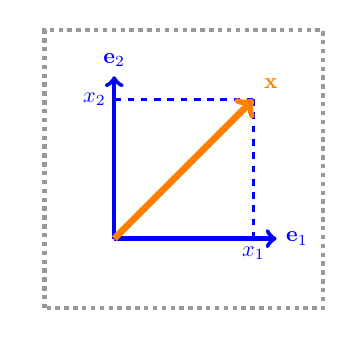
\begin{tikzpicture}[ scale=0.8,]

\tikzstyle{every path}=[line width=2pt]

\begin{axis}[
axis equal,
draw=gray!80,
ymin=-6cm,
ymax=6cm,
xmin=-6cm,
xmax=6cm,
height=6cm,
width=6cm,
%axis line style={draw=none},
axis line style={dotted},
tick style={draw=none},
xticklabels={,,},
yticklabels={,,},
%scale only axis
]


\draw[blue,line width=2pt,->] (axis cs:-3cm,-3cm) -- (axis cs:4cm,-3cm) node[right]{${\bf e}_1$};
\draw[blue,line width=2pt,->] (axis cs:-3cm,-3cm) -- (axis cs:-3cm,4cm) node[above]{${\bf e}_2$};

\draw[blue,line width=1pt,dashed] (axis cs:3cm,-3cm) node[below]{$x_1$} -- (axis cs:3cm,3cm);
\draw[blue,line width=1pt,dashed] (axis cs:-3cm,3cm) node[left]{$x_2$} -- (axis cs:3cm,3cm);

\draw[orange,line width=3pt,->] (axis cs:-3cm,-3cm) -- (axis cs:3cm,3cm) node[above right]{${\bf x}$};


\end{axis}

\end{tikzpicture}
&
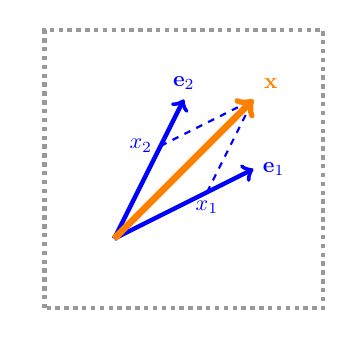
\begin{tikzpicture}[ scale=0.8,]

\tikzstyle{every path}=[line width=2pt]

\begin{axis}[
axis equal,
draw=gray!80,
ymin=-6cm,
ymax=6cm,
xmin=-6cm,
xmax=6cm,
height=6cm,
width=6cm,
%axis line style={draw=none},
axis line style={dotted},
tick style={draw=none},
xticklabels={,,},
yticklabels={,,},
%scale only axis
]


\draw[blue,line width=2pt,->] (axis cs:-3cm,-3cm) -- (axis cs:3cm,-0cm) node[right]{${\bf e}_1$};
\draw[blue,line width=2pt,->] (axis cs:-3cm,-3cm) -- (axis cs:0cm,3cm) node[above]{${\bf e}_2$};

\draw[blue,line width=1pt,dashed] (axis cs:1cm,-1cm) node[below]{$x_1$} -- (axis cs:3cm,3cm);
\draw[blue,line width=1pt,dashed] (axis cs:-1cm,1cm) node[left]{$x_2$} -- (axis cs:3cm,3cm);

\draw[orange,line width=3pt,->] (axis cs:-3cm,-3cm) -- (axis cs:3cm,3cm) node[above right]{${\bf x}$};


\end{axis}

\end{tikzpicture}
\\
(c)&(d)\\
\end{tabular}
\end{center}
\end{figure}

Elementary high school tutorials often condition students into believing that the components of the vector
``is'' the vector, rather than emphasizing that these components {\em represent} or {\em encode}
the vector with respect to some (mostly implicitly assumed) basis.
A similar situation occurs in many introductions to quantum theory,
where the span
(i.e., the one-dimensional linear subspace spanned by that vector)
\index{span}
$\{
{\bf y}
\mid
{\bf y} = \alpha {\bf x}, \alpha \in {\Bbb C}
\}$, or, equivalently,  for orthogonal projections,
the {\em projection} (i.e., the projection operator; see also page \pageref{2011-m-projec})
\index{projection}
$\textsf{\textbf{E}}_{\bf x} \equiv {\bf x} \otimes {\bf x}^\dagger  \equiv \vert {\bf x} \rangle \langle {\bf x}\vert$
corresponding to a unit (of length $1$) vector ${\bf x}$
often is identified with that vector.
In many instances, this is a great help and,
if administered properly, is consistent and fine (at least for all practical purposes).

The  Cartesian  standard basis in $n$-dimensional complex space ${\Bbb C}^n$
\index{Cartesian basis}
\index{standard basis}
is the set of (usually ``straight'')
vectors $x_i, i=1, \ldots , n$, of ``unit length''
-- the unit is conventional and thus needs to be fixed as operationally precisely as possible,
such as in the {\em International System of Units (SI)}
\marginnote{In the {\em International System of Units (SI)}
\index{International System of Units}
the ``second'' as the unit of time is defined to be the duration of 9 192 631 770 periods of the radiation corresponding to the transition
between the two hyperfine levels of the ground state of the cesium 133 atom.
The `` meter'' as the unit of length is defined to be the length of the path traveled by light in vacuum during a time interval
of 1/299 792 458 of a second
--
or, equivalently,
as light travels 299 792 458 meters per second,
a duration in which 9 192 631 770 transitions between two orthogonal quantum states of a cesium 133 atom occur
--
during
9 192 631 770/299 792 458 $\approx 31$ transitions of two orthogonal quantum states of a cesium 133 atom.
Thereby, the speed of light in the vacuum is fixed at exactly 299 792 458 meters per second; see also \bibentry{peres-84}.}
--
represented by $n$-tuples,
defined by the condition that the $i$'th coordinate of the $j$'th basis vector
${\bf e}_j$ is given by $\delta_{ij}$.
Likewise, $\delta_{ij}$ can be interpreted as the  $j$'th coordinate of the $i$'th basis vector.
Thereby $\delta_{ij}$ is the Kronecker delta function
\index{Kronecker delta function}
\begin{equation}
\delta_{ij} =\delta_{ji} =\begin{cases}
0  &\text{ for }i\neq j , \\
1  &\text{ for }i = j.
\end{cases}
\end{equation}
Thus we can represent the basis vectors by
\begin{equation}
\begin{split}
\vert {\bf e}_1 \rangle \equiv {\bf e}_1 \equiv \begin{pmatrix}1\\ 0\\ \vdots\\ 0\end{pmatrix},\quad
\vert {\bf e}_2 \rangle \equiv {\bf e}_2 \equiv \begin{pmatrix}0\\ 1\\ \vdots\\ 0\end{pmatrix},\quad
\ldots\quad
\vert {\bf e}_n \rangle \equiv {\bf e}_n \equiv \begin{pmatrix}0\\ 0\\ \vdots\\ 1\end{pmatrix}.
\end{split}
\label{2016-m-fdvs-csb}
\end{equation}


In terms of these standard base vectors, every vector ${\bf x}$
can be written as a linear combination -- in quantum physics, this is called
{\em coherent superposition}
\index{coherent superposition}
\index{superposition}
\begin{equation}
\vert {\bf x} \rangle \equiv {\bf x} = \sum_{i=1}^n x_i{\bf e}_i \equiv  \sum_{i=1}^n x_i \vert {\bf e}_i \rangle
\equiv
\begin{pmatrix}x_1\\x_2\\ \vdots \\ x_n\end{pmatrix}
\label{2016-m-fdvs-rv0}
\end{equation}
with respect  to the basis
${\frak B}= \{ {\bf e}_1 ,
  {\bf e}_2   ,
\ldots ,
 {\bf e}_n
\}$.

With the notation\marginnote{For reasons demonstrated later in Equation~(\ref{2015-m-ch-fdlvs-uniascolv})
$\textsf{\textbf{U}}$ is a unitary matrix, that is,
$\textsf{\textbf{U}}^{-1}=\textsf{\textbf{U}}^\dagger= \overline{\textsf{\textbf{U}}}^\intercal $,
where the overline stands for complex conjugation $\overline{u}_{ij}$ of the entries $u_{ij}$ of $\textsf{\textbf{U}}$, and
the superscript ``$\intercal$'' indicates transposition; that is, $\textsf{\textbf{U}}^\intercal $ has entries $u_{ji}$.
}
defined by
\begin{equation}
\begin{split} X = \begin{pmatrix}
x_1, x_2, \ldots , x_n
\end{pmatrix}^\dagger
\textrm{, and }
\\
\textsf{\textbf{U}} =
\begin{pmatrix}{\bf e}_1,{\bf e}_2, \ldots , {\bf e}_n\end{pmatrix}
\equiv
\begin{pmatrix} \vert {\bf e}_1\rangle ,\vert {\bf e}_2 \rangle ,  \ldots , \vert {\bf e}_n\rangle \end{pmatrix}
,
\label{2016-m-fdvs-not}
\end{split}
\end{equation}
such that  $u_{ij} = e_{i,j}$ is the $j$th component of the $i$th vector,
Equation~(\ref{2016-m-fdvs-rv0}) can be written
in ``Euclidean dot product notation,''
that is,
``column times row''
and
``row times column'' (the dot is usually omitted)
\begin{equation}
\begin{split}
\vert {\bf x} \rangle \equiv {\bf x} =
\begin{pmatrix}{\bf e}_1,{\bf e}_2, \ldots , {\bf e}_n\end{pmatrix}
\begin{pmatrix} x_1\\x_2\\ \vdots \\ x_n \end{pmatrix}
\equiv
\begin{pmatrix} \vert {\bf e}_1\rangle ,\vert {\bf e}_2 \rangle ,  \ldots , \vert {\bf e}_n\rangle \end{pmatrix}
\begin{pmatrix} x_1\\x_2\\ \vdots \\ x_n \end{pmatrix} \equiv
\\
\equiv
\begin{pmatrix}
{\bf e}_{1,1} &   {\bf e}_{2,1}  &  \cdots &  {\bf e}_{n,1}\\
{\bf e}_{1,2} &   {\bf e}_{2,2}  &  \cdots &  {\bf e}_{n,2}\\
\cdots  & \cdots  &  \ddots &  \cdots \\
{\bf e}_{1,n} &   {\bf e}_{2,n}  &  \cdots &  {\bf e}_{n,n}\\
\end{pmatrix}
\begin{pmatrix} x_1\\x_2\\ \vdots \\ x_n \end{pmatrix}
\equiv
\textsf{\textbf{U}} X
 .
\label{2016-m-fdvs-rv}
\end{split}
\end{equation}
Of course, with the Cartesian standard basis (\ref{2016-m-fdvs-csb}), $\textsf{\textbf{U}} = \mathbb{1}_n$, but
(\ref{2016-m-fdvs-rv}) remains valid for general bases.


In (\ref{2016-m-fdvs-rv}) the identification of the tuple
$ X = \begin{pmatrix}
x_1, x_2, \ldots , x_n
\end{pmatrix}^\intercal
$
containing the vector components $x_i$
with the vector $\vert {\bf x} \rangle \equiv {\bf x}$
really means
``coded {\em with respect}, or {\em relative},  to the basis ${\frak B}=\{{\bf e}_1,{\bf e}_2, \ldots , {\bf e}_n\}$.''
Thus in what follows, we shall often identify the column vector
$
\begin{pmatrix}
x_1, x_2, \ldots , x_n
\end{pmatrix}^\intercal
$
containing the coordinates of the vector
with the vector ${\bf x}\equiv \vert {\bf x} \rangle$, but we always need to keep in mind that
the tuples of coordinates are defined only with respect to a particular basis
$\{ {\bf e}_1,{\bf e}_2, \ldots , {\bf e}_n \}$; otherwise these numbers lack any meaning whatsoever.

Indeed, with respect to some arbitrary  basis ${\frak B}=\{
{\bf f}_1, \ldots , {\bf f}_n\}$ of some $n$-dimensional vector space ${\frak V}$
with the base vectors ${\bf f}_i$, $1\le i\le n$, every vector ${\bf x}$ in  ${\frak V}$
can be written as a unique linear combination
\begin{equation}
 \vert {\bf x} \rangle \equiv {\bf x} = \sum_{i=1}^n x_i{\bf f}_i
\equiv
\sum_{i=1}^n x_i \vert {\bf f}_i \rangle
\equiv \begin{pmatrix} x_1\\x_2\\ \vdots \\ x_n \end{pmatrix}
\end{equation}
with respect to the basis  ${\frak B}=\{
{\bf f}_1, \ldots , {\bf f}_n\}$.

{\color{OliveGreen}
\bproof
The uniqueness of the coordinates is proven indirectly by {\em reductio ad absurdum:}
Suppose there is another decomposition
${\bf x} = \sum_{i=1}^n y_i{\bf f}_i = (y_1,y_2, \ldots , y_n) $;
then by subtraction, $0 = \sum_{i=1}^n (x_i-y_i) {\bf f}_i = (0,0, \ldots , 0)$.
Since the basis vectors ${\bf f}_i$ are linearly independent,
this can only be valid if all coefficients in the summation  vanish;
thus $x_i-y_i=0$ for all $1\le i\le n$; hence finally  $x_i=y_i$ for all $1\le i\le n$.
This is in contradiction with our assumption that the coordinates $x_i$ and $y_i$
(or at least some of them) are different.
Hence the only consistent alternative is the assumption that, with respect to a given basis, the coordinates are uniquely determined.
\eproof
}

A  set    ${\frak B} = \{ {\bf a}_1, \ldots , {\bf a}_n\}$
of  vectors   of the inner product space $\frak V$
is {\em orthonormal}
\index{orthonormal}
if, for all
 ${\bf a}_i\in\frak B$ and
 ${\bf a}_j\in\frak B$,
it follows that
\begin{equation}
\langle {\bf a}_i \mid {\bf a}_j \rangle =\delta_{ij}.
\label{2013-m-ch-fdvs-orthonorm}
\end{equation}
Any such set is called {\em complete}
\index{completeness}
if it is not a subset of any larger orthonormal set of vectors of $\frak V$.
Any complete set is a basis.
If, instead of Equation~(\ref{2013-m-ch-fdvs-orthonorm}),
$\langle {\bf a}_i \mid {\bf a}_j \rangle = \alpha_i \delta_{ij}$
with nonzero factors $\alpha_i$, the set is called {\em orthogonal}.


\section{Finding orthogonal bases from nonorthogonal ones}
\label{2019-mm-ch-fdvs-GS}

A {\em Gram-Schmidt process}\cite{Leon-MR3054730}
or {\em Householder orthonormalization}
is a systematic method for orthonormalising a set of vectors
\index{Gram-Schmidt process}
\index{Householder orthonormalization}
\index{scalar product}
\index{inner product}
in a space equipped with a {\em scalar product,}
or by a synonym preferred in mathematics, {\em inner product.}


The Gram-Schmidt process or Householder
orthonormalization\marginnote{The Householder orthonormalization will be dealt with in Section~\ref{2021-m-ch-hposholder} on page~\pageref{2021-m-ch-hposholder}.}
takes a finite, linearly independent set
of base vectors
and generates an orthonormal basis that spans the same (sub)space as the original set.

The general method of the Gram-Schmidt process  is to start with the original basis,
say,  \\
$\{
{\bf x}_1,
{\bf x}_2,
{\bf x}_3,
\ldots ,
{\bf x}_n
\}$,
and generate a new orthogonal basis
by
\begin{equation}
\begin{split}
{\bf y}_1={\bf x}_1,\\
{\bf y}_2={\bf x}_2 - P_{{\bf y}_1}({\bf x}_2),\\
{\bf y}_3={\bf x}_3 - P_{{\bf y}_1}({\bf x}_3)- P_{{\bf y}_2}({\bf x}_3),\\
 \vdots \\
{\bf y}_n={\bf x}_n -\sum_{i=1}^{n-1} P_{{\bf y}_i}({\bf x}_n),
\end{split}
\end{equation}
where
\marginnote{The scalar or inner product
$\langle {\bf x}\vert {\bf y} \rangle$ of two vectors
${\bf x}$ and ${\bf y}$ is defined on page \pageref{2011-m-scalarproduct}.
In Euclidean  space such as ${\Bbb R}^n$,
one often identifies the ``dot product''
${\bf x}\cdot {\bf y} =x_1y_1+ \cdots +x_ny_n$
of two vectors ${\bf x}$ and $ {\bf y}$ with their scalar or inner product.}
$\{
{\bf y}_1,
{\bf y}_2,
{\bf y}_3,
\ldots ,
{\bf y}_n
\}$
\begin{equation}
P_{{\bf y}}({\bf x}) =
\frac{\langle {\bf y} \vert  {\bf x}\rangle }
{\langle {\bf y}\vert {\bf y} \rangle }
{\bf y}
,\textrm{ and }
P_{{\bf y}}^\perp ({\bf x}) = {\bf x} -
\frac{\langle {\bf y} \vert  {\bf x}\rangle }
{\langle {\bf y}\vert {\bf y} \rangle }
{\bf y}
\end{equation}
are the orthogonal projections of ${\bf x}$ onto ${\bf y}$ and ${\bf y}^\perp$, respectively
(the latter is mentioned for the sake of completeness and is not required here).
\label{2011-m-gsp}
Note that these orthogonal projections are idempotent
\index{idempotence}
%(i.e., $p^2=p(p)=p$ and $(p^\perp)^2=p^\perp (p^\perp)=p^\perp$)
and mutually orthogonal; that is,
\begin{equation}
\begin{split}
P_{{\bf y}}^2({\bf x})  = P_{{\bf y}}(P_{{\bf y}}({\bf x}) ) =
\frac{\langle {\bf y}\vert {\bf y} \rangle }{\langle {\bf y}\vert {\bf y} \rangle }
\frac{\langle {\bf y} \vert  {\bf x}\rangle }{\langle {\bf y}\vert {\bf y} \rangle }
{\bf y} =P_{{\bf y}}({\bf x}),  \\
%
(P_{{\bf y}}^\perp)^2({\bf x})  = P_{{\bf y}}^\perp(P_{{\bf y}}^\perp({\bf x}) ) =
{\bf x}- \frac{\langle {\bf y} \vert  {\bf x}\rangle }{\langle {\bf y}\vert {\bf y} \rangle }{\bf y}
-\left(
\frac{\langle {\bf y} \vert  {\bf x}\rangle }{\langle {\bf y}\vert {\bf y} \rangle }
-
\frac{\langle {\bf y}\vert {\bf y} \rangle \langle {\bf y} \vert  {\bf x}\rangle
}{\langle {\bf y}\vert {\bf y} \rangle^2 }
\right)
{\bf y}
=P_{{\bf y}}^\perp({\bf x}),  \\
P_{{\bf y}}(P_{{\bf y}}^\perp({\bf x}) ) =  P_{{\bf y}}^\perp(P_{{\bf y}}({\bf x}) ) =
\frac{\langle {\bf y} \vert  {\bf x}\rangle}{\langle {\bf y}\vert {\bf y} \rangle }{\bf y}
-
\frac{\langle {\bf y}\vert {\bf y} \rangle \langle {\bf y} \vert  {\bf x}\rangle }{\langle {\bf y}\vert {\bf y} \rangle^2 }
{\bf y}
=0.
\end{split}
\end{equation}
For a more general discussion of projections, see also page \pageref{2011-m-projec}.

Subsequently, in order to obtain an orthonormal basis,
one can divide every basis vector by its length.

{\color{OliveGreen}
\bproof
The idea of the proof is as follows (see also Section~7.9 of Ref.\cite{Greub75}).
In order to generate an orthogonal basis from a nonorthogonal one,
the first vector of the old basis is identified with the first vector of the new basis;
that is ${\bf y}_1={\bf x}_1$.
Then, as depicted in Figure~\ref{2012-m-fdvs-ideaofGS}, the second vector of the new basis is obtained by
taking the second vector of the old basis and
subtracting its projection on the first vector of the new basis.
\begin{marginfigure}%
{\color{black}
\begin{center}%
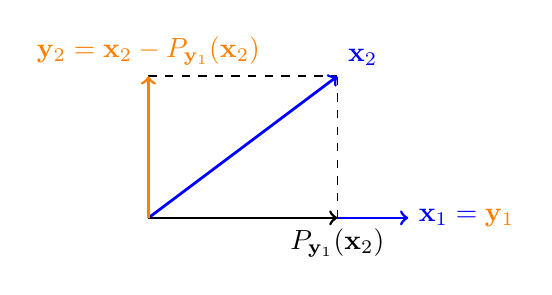
\begin{tikzpicture}[ scale=0.6]



\draw[black,line width=0.5pt,dashed] (0cm,3cm) -- (4cm,3cm);

\draw[black,line width=0.5pt,dashed] (4cm,0cm) -- (4cm,3cm);

\draw[blue,line width=1pt,->] (0cm,0cm) -- (5.5cm,0cm) node[right]{${\bf x}_1= {\color{orange}{\bf y}_1}$};

\draw[blue,line width=1pt,->] (0cm,0cm) -- (4cm,3cm) node[above right]{${\bf x}_2$};

\draw[black,line width=1pt,->] (0cm,0cm) -- (4cm,0cm) node[below]{$P_{{\bf y}_1}({\bf x}_2)$};

\draw[orange,line width=1pt,->] (0cm,0cm) -- (0cm,3cm) node[above]{${\bf y}_2= {\bf x}_2 -P_{{\bf y}_1}({\bf x}_2)$};



\end{tikzpicture}
\end{center}%
\caption{\label{2012-m-fdvs-ideaofGS}Gram-Schmidt construction for two nonorthogonal vectors ${\bf x}_1$ and ${\bf x}_2$,
yielding two  orthogonal vectors ${\bf y}_1$ and ${\bf y}_2$.}
}
\end{marginfigure}
More precisely, take the Ansatz
\begin{equation}
{\bf y}_2={\bf x}_2 + \lambda  {\bf y}_1,
\end{equation}
thereby determining the arbitrary scalar $\lambda$ such that
${\bf y}_1$
and
${\bf y}_2$
are orthogonal; that is,
$\langle{\bf y}_2 \vert  {\bf y}_1\rangle =0$.
This yields
\begin{equation}
\langle {\bf y}_1\vert  {\bf y}_2 \rangle
=\langle {\bf y}_1 \vert {\bf x}_2 \rangle
+ \lambda
\langle {\bf y}_1\vert  {\bf y}_1\rangle =0,
\end{equation}
and thus, since ${\bf y}_1 \neq 0$,
\begin{equation}
\lambda =
-
\frac{\langle {\bf y}_1 \vert {\bf x}_2 \rangle}
{\langle {\bf y}_1\vert {\bf y}_1 \rangle} .
\end{equation}
To obtain the third vector ${\bf y}_3$ of the new basis,
take the Ansatz
\begin{equation}
{\bf y}_3={\bf x}_3 + \mu  {\bf y}_1  + \nu  {\bf y}_2,
\label{2012-m-ch-gs1}
\end{equation}
and require that it is orthogonal to the two previous orthogonal basis vectors
${\bf y}_1$
and
${\bf y}_2$;
that is
$\langle {\bf y}_1\vert {\bf y}_3 \rangle =\langle  {\bf y}_2\vert{\bf y}_3  \rangle =0$.
We already know that $\langle {\bf y}_1\vert {\bf y}_2 \rangle = 0$.
Consider the scalar products of ${\bf y}_1$
and ${\bf y}_2$
with the {\it Ansatz} for ${\bf y}_3$ in Equation~(\ref{2012-m-ch-gs1}); that is,
\begin{equation}
\begin{split}
\langle {\bf y}_1\vert {\bf y}_3\rangle
=
\langle {\bf y}_1 \vert {\bf x}_3 \rangle + \mu  \langle {\bf y}_1\vert {\bf y}_1 \rangle  + \nu   \underbrace{\langle {\bf y}_1\vert {\bf y}_2\rangle}_{=0}
 =0,
\end{split}
\end{equation}
and
\begin{equation}
\begin{split}
\langle{\bf y}_2 \vert {\bf y}_3\rangle =\langle {\bf y}_2\vert  {\bf x}_3\rangle + \mu \underbrace{ \langle {\bf y}_2\vert {\bf y}_1 \rangle}_{=0}   + \nu \langle {\bf y}_2\vert {\bf y}_2\rangle
  =0.
\end{split}
\end{equation}
As a result,
\begin{equation}
\mu = -  \frac{\langle {\bf y}_1 \vert {\bf x}_3 \rangle}
{\langle {\bf y}_1\vert {\bf y}_1 \rangle},\quad
\nu =- \frac{\langle {\bf y}_2\vert  {\bf x}_3\rangle}
{\langle {\bf y}_2 \vert {\bf y}_2 \rangle}.
\end{equation}
A generalization of this construction
for all the other new base vectors
${\bf y}_3, \ldots ,  {\bf y}_n$, and thus a proof by complete induction,
proceeds by a generalized construction.
\eproof
}

{\color{blue}
\bexample
Consider, as an example, the standard Euclidean scalar product denoted by ``$\cdot$''
and the basis
$\left\{\begin{pmatrix}0\\1\end{pmatrix},\begin{pmatrix}1\\1\end{pmatrix}\right\}$.
Then two orthogonal bases are obtained by taking
\begin{itemize}
\item[(i)]
either the basis vector
$\begin{pmatrix}0\\1\end{pmatrix}$, together with
$
\begin{pmatrix}1\\1\end{pmatrix} -
\frac{\begin{pmatrix}1\\1\end{pmatrix}\cdot \begin{pmatrix}0\\1\end{pmatrix}}{\begin{pmatrix}0\\1\end{pmatrix}\cdot \begin{pmatrix}0\\1\end{pmatrix}} \begin{pmatrix}0\\1\end{pmatrix} = \begin{pmatrix}1\\0\end{pmatrix},
$
\item[(ii)]
or the basis vector
$\begin{pmatrix}1\\1\end{pmatrix}$, together with
$
\begin{pmatrix}0\\1\end{pmatrix} -
\frac{\begin{pmatrix}0\\1\end{pmatrix}\cdot \begin{pmatrix}1\\1\end{pmatrix}}{\begin{pmatrix}1\\1\end{pmatrix}\cdot \begin{pmatrix}1\\1\end{pmatrix}} \begin{pmatrix}1\\1\end{pmatrix} = \frac{1}{2}\begin{pmatrix}-1\\1\end{pmatrix}. \textrm{\eexample}
$
\end{itemize}
}





\section{Dual space}
\label{2011-m-dvs}
\marginnote{For proofs and additional information see {\S}13--15 in~\bibentry{halmos-vs}.}

Every vector space ${\frak V}$
has a corresponding {\em dual vector space}
\index{dual vector space}
\index{dual space}
(or just {\em dual space})   ${\frak V}^\ast$
consisting of all linear functionals on ${\frak V}$.

A {\em linear functional}
\index{linear functional}
on a vector space ${\frak V}$ is a scalar-valued linear function ${\bf y}$
defined for every vector   ${\bf x} \in {\frak V}$, with the linear property that\marginnote{
Although
the linear functional ${\bf y}$ is written in vector notation,
elements of its codomain or set of destination or outputs are scalars
(note also that elements of its  domain or set of departure or inputs are vectors of a vector space).
The vector notation has been chosen because every such linear functional ${\bf y}$
can be represented as a vector in a linear vector space
spanned by the dual basis
defined in Equation~(\ref{2011-m-Dualbasis-e1}).
An example (with scalar domain and codomain) are polynomials $x^l$ or Legendre polynomials $P_l$ (cf. Section~\ref{2013-m-sf-lp})
\index{Legendre polynomial}
with $i\in \mathbb{N}_0$, spanning an infinite dimensional vector space.
}
\begin{equation}
{\bf y} (\alpha_1 {\bf x}_1 +\alpha_2 {\bf x}_2)
=
\alpha_1 {\bf y} ({\bf x}_1) +\alpha_2 {\bf y} ({\bf x}_2) .
\end{equation}

{\color{blue}
\bexample
For example,
let ${\bf x} = (x_1,\ldots , x_n)$, and
take
${\bf y} ({\bf x}) =x_1$.

For another example,
let again ${\bf x} = (x_1,\ldots , x_n)$, and
let $\alpha_1,\ldots , \alpha_n \in {\Bbb C}$ be scalars; and
take
${\bf y} ({\bf x}) =\alpha_1 x_1 + \cdots +\alpha_n x_n$.

The following supermarket example has been
communicated to me by Hans Havlicek:\cite{havlicek-priv3}
suppose you visit a supermarket, with a variety of products therein.
Suppose further that you select some items and collect them in a cart or trolley.
Suppose further that, in order to complete your purchase, you finally go to the cash desk,
where the sum total of your purchase is computed from the price-per-product information stored
in the memory of the cash register.

In this example, the vector space can be identified with all conceivable configurations of products in a cart or trolley.
Its dimension is determined by the number of different, mutually distinct products in the supermarket.
Its ``base vectors'' can be identified with the mutually distinct products in the supermarket.
The respective functional is the computation of the price of any such purchase.
It is based on a particular price information.
Every such price information contains one price per item for all mutually distinct products.
The dual space consists of all conceivable price details.
The number of respective basis vectors---encoded as price-per-product---needs to be the same as the number of products.
Therefore, the dimensions of both all product configurations ``spanning'' the vector space,
as well as of all possible prices rendered, needs to be the same.
\eexample
}


We adopt a doublesquare bracket notation ``$\llbracket \cdot , \cdot \rrbracket$''
for the functional


\begin{equation}
{\bf y} ({\bf x})
=
\llbracket {\bf x},{\bf y}\rrbracket .
\end{equation}

The set of linear functionals is closed with respect to
the addition of two or more of such functionals, as well as multiplication of scalars with a functional;
that is,
\begin{equation}
(a {\bf y} + b {\bf z}) ({\bf x})
=
  a {\bf y} ({\bf x}) + b {\bf z} ({\bf x})
.
\end{equation}
Together with the ``zero functional''
(mapping every argument to zero), as well as other algebrac properties,
this induces a kind of linear vector space structure, where the ``vectors''
are identified with the linear functionals.
This vector space will be called {\em dual space} ${\frak V}^\ast $.
\index{dual space}


As a result, this ``bracket'' functional is
{\em bilinear} in its two arguments; that is,
\begin{equation}
\llbracket  \alpha_1 {\bf x}_1 +\alpha_2 {\bf x}_2, {\bf y}\rrbracket
=
\alpha_1 \llbracket {\bf x}_1 ,{\bf y}\rrbracket   +\alpha_2  \llbracket {\bf x}_2,{\bf y}\rrbracket ,
\end{equation}
and
\begin{equation}
\llbracket
{\bf x}, \alpha_1 {\bf y}_1 +\alpha_2 {\bf y}_2
\rrbracket
=
\alpha_1
\llbracket {\bf x},{\bf y}_1 \rrbracket
+
\alpha_2
\llbracket {\bf x},{\bf y}_2\rrbracket .
\end{equation}
\marginnote{The square bracket can be identified with the scalar dot product
$\llbracket  {\bf x},{\bf y} \rrbracket  = \langle {\bf x}\mid {\bf y}\rangle$
only for Euclidean
vector spaces ${\Bbb R}^n$, since for complex spaces this would no longer be positive definite.
That is, for Euclidean
vector spaces ${\Bbb R}^n$ the inner or scalar product is bilinear.
}


Because of linearity, we can completely characterize an arbitrary linear functional
${\bf y} \in {\frak V}^\ast $ by its values of the vectors of some basis of ${\frak V}$:
If we know the functional value on the basis vectors in ${\frak B}$, we know the functional
on all elements of the vector space ${\frak V}$.
If ${\frak V}$ is an $n$-dimensional vector space, and if ${\frak B} = \{{\bf f}_1,\ldots , {\bf f}_n\}$
is a basis of  ${\frak V}$, and if
$\{\alpha_1, \ldots ,\alpha_n\}$  is any set of $n$ scalars, then there is
a unique linear functional ${\bf y}$  on  ${\frak V}$ such that
$ \llbracket  {\bf f}_i, {\bf y}\rrbracket  = \alpha_i $ for all $0\le i \le n$.

{\color{OliveGreen}
\bproof
A constructive proof  of this theorem can be given as follows:
Because every ${\bf x}\in {\frak V}$
can be written as a linear combination $ {\bf x} = x_1 {\bf f}_1 +\cdots + x_n {\bf f}_n$
of the basis vectors of ${\frak B} = \{{\bf f}_1,\ldots , {\bf f}_n\}$
in one and only one (unique) way, we obtain for any arbitrary linear functional ${\bf y} \in {\frak V}^\ast $  a unique decomposition
in terms of the basis vectors of  ${\frak B} = \{{\bf f}_1,\ldots , {\bf f}_n\}$; that is,
\begin{equation}
\llbracket {\bf x},{\bf y}\rrbracket
=
x_1 \llbracket {\bf f}_1 ,{\bf y}\rrbracket  +\cdots + x_n \llbracket {\bf f}_n ,{\bf y}\rrbracket  .
\end{equation}
By identifying  $\llbracket {\bf f}_i ,{\bf y}\rrbracket =\alpha_i$ we obtain
\begin{equation}
\llbracket {\bf x},{\bf y}\rrbracket
=
x_1 \alpha_1 +\cdots + x_n \alpha_n .
\end{equation}
\eproof
}

Conversely, if we {\em define} ${\bf y}$ by $\llbracket {\bf x},{\bf y}\rrbracket  =\alpha_1  x_1+ \cdots +\alpha_n x_n$, then ${\bf y}$
can be interpreted as a linear functional in ${\frak V}^\ast$ with $\llbracket {\bf f}_i,{\bf y}\rrbracket  = \alpha_i$.

If we introduce a {\em dual basis}
by requiring that $\llbracket {\bf f}_i,  {\bf f}_j^\ast \rrbracket =\delta_{ij}$ [cf. Equation~(\ref{2011-m-Dualbasis-e1})],
then the coefficients $\llbracket {\bf f}_i ,{\bf y}\rrbracket  = \alpha_i$,
$1\le i \le n$, can be interpreted
as the {\em coordinates} of the linear functional ${\bf y}$ with respect to the dual
basis ${\frak B}^\ast$, such that or,
relative to the dual basis defined in the next Section~\ref{2011-m-Dualbasis},
${\bf y}=\sum_i \alpha_i {\bf f}_i^\ast$, or, with respect to the dual basis,
${\bf y}=(\alpha_1,\alpha_2,\ldots , \alpha_n)$.

Likewise, as will be shown in (\ref{2014-m-ch-fdlvs-kju}),
$
x_i =
 \llbracket {\bf x},{\bf f}_i^\ast \rrbracket
$; that is, the vector coordinates can be represented by the functionals of the elements of the dual basis.

The number of such basis vectors---and thus the dimension of the dual space---needs to be the same
as the dimension of the original vector space: because of linearity it is necessary and sufficient to know all functional values on the
vectors of the basis of the original space.


{\color{blue}
\bexample
Let us explicitly construct an example of a linear functional $\varphi ({\bf x})\equiv \llbracket {\bf x},\varphi\rrbracket $ that is defined
on all vectors ${\bf x}=
\alpha {\bf e}_1
+
\beta {\bf e}_2
$
of a two-dimensional vector space with the basis $\{{\bf e}_1, {\bf e}_2 \}$
by enumerating its ``performance on the basis vectors''  ${\bf e}_1=\begin{pmatrix}1,0\end{pmatrix}^\intercal$
and ${\bf e}_2=\begin{pmatrix}0,1\end{pmatrix}^\intercal$;
more explicitly,  say, for an example's sake,
$\varphi ({\bf e}_1 ) \equiv \llbracket  {\bf e}_1,\varphi \rrbracket  = 2$ and
$\varphi ({\bf e}_2 ) \equiv \llbracket  {\bf e}_2,\varphi \rrbracket  = 3$.
Therefore, for example for the vector $\begin{pmatrix}5,7\end{pmatrix}^\intercal$,
$\varphi \left(\begin{pmatrix}5,7\end{pmatrix}^\intercal \right)
\equiv \left\llbracket \begin{pmatrix}5,7\end{pmatrix}^\intercal,
\varphi \right\rrbracket  = 5 \llbracket {\bf e}_1, \varphi \rrbracket  + 7 \llbracket  {\bf e}_2,\varphi \rrbracket
=10+21=31$.

In general the performance of the linear function on just one vector renders insufficient
information to uniquely define a linear functional of vectors of dimension two or higher:
one needs as many values on mutually
linear independent vectors as there are dimensions for a complete specification of the linear functional.
Take, for example, just one value of $\varphi$ on a single vector, say
${\bf x}=\begin{pmatrix} 5,7 \end{pmatrix}^\intercal$; that is,
$\varphi \left( {\bf x} \right)=31$. If one does not
know the linear functional beforehand,
all one can do is to write $\varphi$ in terms of its components (with respect to the dual basis)
$\varphi = \begin{pmatrix} \varphi_1 ,\varphi_2 \end{pmatrix}$
and evaluate
$\begin{pmatrix} \varphi_1 ,\varphi_2 \end{pmatrix} \cdot \begin{pmatrix} 5,7 \end{pmatrix}^\intercal
= 5\varphi_1 +7\varphi_2 = 31$, which just yields one component of $\varphi$ in terms of the other;
that is, $\varphi_1  = (31-7\varphi_2)/5$.
The components of $\varphi$ (with respect to the dual basis) are uniquely fixed
only by presentation of another value, say
$\varphi \left( {\bf y} \right)=13$,
on another vector
${\bf y}=\begin{pmatrix} 2,3 \end{pmatrix}^\intercal$ not collinear to the first vector ${\bf x}$.
Then
$\begin{pmatrix} \varphi_1 ,\varphi_2 \end{pmatrix} \cdot \begin{pmatrix} 2,3 \end{pmatrix}^\intercal
= 2\varphi_1 +3\varphi_2 = 13$  yields $\varphi_1  = (13-3\varphi_2)/2$.
Equating those two equations for $\varphi_1$ yields
$(31-7\varphi_2)/5=(13-3\varphi_2)/2$ and thus $\varphi_2=3$ and therefore $\varphi_1=2$.


\eexample
}

\subsection{Dual basis}
\label{2011-m-Dualbasis}

We now can define a {\em dual basis}, or, used synonymously, a {\em reciprocal} or {\em contravariant} basis.
\index{dual basis}
\index{reciprocal basis}
\index{contravariant basis}
If ${\frak V}$ is an $n$-dimensional vector space, and if
${\frak B} = \{{\bf f}_1,\ldots , {\bf f}_n\}$
is a basis of  ${\frak V}$,
then there is a unique {\em dual basis}
${\frak B}^\ast
=\{{\bf f}_1^\ast ,\ldots , {\bf f}_n^\ast \}$ in the dual vector space ${\frak V}^\ast $
defined by
\begin{equation}
{\bf f}_j^\ast ({\bf f}_i) =  \llbracket {\bf f}_i,  {\bf f}_j^\ast \rrbracket =\delta_{ij},
\label{2011-m-Dualbasis-e1}
\end{equation}
where  $\delta_{ij}$
is the Kronecker delta function.
The dual space  ${\frak V}^\ast $ spanned by the dual basis ${\frak B}^\ast $ is $n$-dimensional.

In a different notation involving subscripts (lower indices) for (basis) vectors of the base vector space,
and superscripts (upper indices) ${\bf f}^j = {\bf f}_j^\ast $,
for (basis) vectors of the dual vector space,
Equation~(\ref{2011-m-Dualbasis-e1}) can be written as
\begin{equation}
{\bf f}^j ( {\bf f}_i ) = \llbracket {\bf f}_i,{\bf f}^j\rrbracket =\delta_{ij}.
\label{2011-m-Dualbasis-e2}
\end{equation}
Suppose
$g$ is a {\em metric},
\index{metric}
facilitating the translation from vectors of the base vectors into vectors of the dual space and {\it vice versa}
(cf. Section~\ref{2011-m-metrict} on page~\pageref{2011-m-metrict} for a definition and more details),
in particular, ${\bf f}_i =  g_{il}{\bf f}^l$
as well as  ${\bf f}_j^\ast  = {\bf f}^j = g^{jk}{\bf f}_k$.
Then Eqs.~(\ref{2011-m-Dualbasis-e1}) and (\ref{2011-m-Dualbasis-e2}) can be rewritten as
\begin{equation}
\llbracket g_{il} {\bf f}^l, {\bf f}^j\rrbracket     = \llbracket {\bf f}_i, g^{jk} {\bf f}_k\rrbracket   = \delta_{ij}.
\label{2011-m-Dualbasis-e3}
\end{equation}

Note that the vectors ${\bf f}^\ast_i = {\bf f}^i$ of the dual basis can be used to ``retrieve''
or ``extract'' the components of arbitrary vectors
${\bf x} = \sum_j x_j {\bf f}_j$  through
\begin{equation}
{\bf f}^\ast_i ( {\bf x} ) =
{\bf f}^\ast_i \left( \sum_j x_j {\bf f}_j \right) =
\sum_j  x_j {\bf f}^\ast_i \left({\bf f}_j \right) =
\sum_j  x_j \delta_{ij} =
x_i.
\label{2016-m-fdlvs-recoverc}
\end{equation}
Likewise, the basis vectors ${\bf f}_i$ can be used to extract the respective coordinates of any dual vector.



In terms of the inner products of the base vector space and its dual vector space the representation
of the metric
may be defined by
$g_{ij}=g({\bf f}_i,{\bf f}_j)=\langle {\bf f}_i\mid {\bf f}_j\rangle$,
as well as
$g^{ij}=g({\bf f}^i,{\bf f}^j) =\langle {\bf f}^i\mid {\bf f}^j\rangle$, respectively.
Note, however, that the coordinates $g_{ij}$ of
the metric $g$ need not necessarily be positive definite.
For example,  special relativity uses the ``pseudo-Euclidean'' metric
 $g={\rm diag}(+1,+1,+1,-1)$ (or just $g={\rm diag}(+,+,+,-)$), where ``${\rm diag}$''
stands for the {\em diagonal matrix}
\index{diagonal matrix}
with the arguments in the diagonal.
\marginnote{The metric tensor $g_{ij}$ represents a {\em bilinear functional}
$g({\bf x},{\bf y}) =x^iy^j g_{ij}$ that is {\em symmetric}; that is,
$g({\bf x},{\bf y}) = g({\bf y},{\bf x})$
and {\em nondegenerate}; that is, for any nonzero vector ${\bf x}\in {\frak V}$,   ${\bf x}\neq 0$,
there is some  vector  ${\bf y}\in {\frak V}$, so that  $g({\bf x},{\bf y}) \neq 0$.
$g$ also satisfies the triangle
inequality
$\vert\vert {\bf x} -{\bf z} \vert\vert  \le \vert\vert {\bf x} - {\bf y} \vert\vert  + \vert\vert  {\bf y} - {\bf z} \vert\vert $.
}




In a real Euclidean vector space ${\Bbb R}^n$
with the dot product as the scalar product,
the dual basis of an orthogonal basis  is also orthogonal, and contains vectors with the same directions,
although with {\em reciprocal length} (thereby explaining the wording ``reciprocal basis'').
Moreover, for an orthonormal basis, the basis vectors are uniquely identifiable by
${\bf e}_i \longrightarrow {\bf e}_i^* = {\bf e}_i^\intercal $.
This identification can only be made for orthonormal bases; it is {\em not} true for nonorthonormal bases.

%{\color{OliveGreen} \bproof
%For a proof ask your audience or a wizard \frownie


A ``reverse construction'' of the elements ${\bf f}_j^\ast $ of the dual basis ${\frak B}^\ast $
-- thereby using the definition ``$\llbracket {\bf f}_i,{\bf y}\rrbracket  = \alpha_i$
for all $1 \le i \le n$''
for any element ${\bf y}$ in ${\frak V}^\ast $ introduced earlier
--
can be given as follows:
for every $1\le j \le n$,
we can {\em define} a vector ${\bf f}_j^\ast $ in the dual basis ${\frak B}^\ast $
by the {\em requirement}   $\llbracket {\bf f}_i,{\bf f}_j^\ast \rrbracket  = \delta_{ij}$.
That is, in words:
the dual basis element, when applied to the elements of the original $n$-dimensional basis,
yields one if and only if  it corresponds to the respective equally indexed basis element;
for all the other $n-1$ basis elements it yields zero.

What remains to be proven is the conjecture that
${\frak B}^\ast  = \{{\bf f}_1^\ast ,\ldots , {\bf f}_n^\ast \}$
is a basis of ${\frak V}^\ast $; that is, that the vectors in ${\frak B}^\ast $ are linear independent,
and that they span ${\frak V}^\ast $.

First observe that ${\frak B}^\ast $ is a set of linear independent vectors,
for if
$ \alpha_1 {\bf f}_1^\ast  + \cdots + \alpha_n {\bf f}_n^\ast =0$, then also
\begin{equation}
 \llbracket {\bf x},\alpha_1 {\bf f}_1^\ast  + \cdots + \alpha_n {\bf f}_n^\ast \rrbracket =
 \alpha_1 \llbracket {\bf x},{\bf f}_1^\ast \rrbracket  + \cdots + \alpha_n \llbracket {\bf x},{\bf f}_n^\ast \rrbracket =
0
\end{equation}
for arbitrary ${\bf x}\in {\frak V}$.
In particular, by identifying ${\bf x}$ with ${\bf f}_i \in {\frak B}$, for $1 \le i \le n$,
\begin{equation}
 \alpha_1 \llbracket {\bf f}_i,{\bf f}_1^\ast \rrbracket  + \cdots + \alpha_n \llbracket {\bf f}_i,{\bf f}_n^\ast \rrbracket = \alpha_j \llbracket {\bf f}_i,{\bf f}_j^\ast \rrbracket  = \alpha_j \delta_{ij} = \alpha_i=
0.
\end{equation}

Second,  every ${\bf y} \in {\frak V}^\ast $ is a linear combination of elements in
${\frak B}^\ast  = \{{\bf f}_1^\ast ,\ldots , {\bf f}_n^\ast \}$, because by
starting from
$\llbracket {\bf f}_i,  {\bf y}\rrbracket =\alpha_i$,
with
$ {\bf x} = x_1 {\bf f}_1 +\cdots + x_n {\bf f}_n$
we obtain
\begin{equation}
 \llbracket {\bf x},{\bf y}\rrbracket
= x_1 \llbracket {\bf f}_1,{\bf y}\rrbracket  +\cdots + x_n \llbracket {\bf f}_n,{\bf y}\rrbracket
= x_1 \alpha_1 +\cdots + x_n \alpha_n.
\label{2014-m-fdvs-ba}
\end{equation}
Note that , for arbitrary  ${\bf x}\in {\frak V}$,
\begin{equation}
 \llbracket {\bf x},{\bf f}_i^\ast \rrbracket
= x_1 \llbracket {\bf f}_1,{\bf f}_i^\ast \rrbracket  +\cdots + x_n \llbracket {\bf f}_n,{\bf f}_i^\ast \rrbracket =  x_j \llbracket {\bf f}_j,{\bf f}_i^\ast \rrbracket =  x_j \delta_{ji}=  x_i,
\label{2014-m-ch-fdlvs-kju}
\end{equation}
and by substituting $\llbracket {\bf x},{\bf f}_i\rrbracket $ for $x_i$ in Equation~(\ref{2014-m-fdvs-ba}) we obtain
\begin{equation}
\begin{split}
 \llbracket {\bf x},{\bf y}\rrbracket  =
 x_1\alpha_1 +\cdots + x_n \alpha_n \\
= \llbracket {\bf x},{\bf f}_1\rrbracket  \alpha_1 +\cdots + \llbracket {\bf x},{\bf f}_n\rrbracket  \alpha_n  \\
= \llbracket {\bf x},\alpha_1 {\bf f}_1 +\cdots + \alpha_n{\bf f}_n\rrbracket  ,
\label{2014-m-fdvs-ba1}
\end{split}
\end{equation}
and therefore ${\bf y} =\alpha_1 {\bf f}_1 +\cdots + \alpha_n{\bf f}_n=\alpha_i{\bf f}_i$.

%\eproof }

How can one determine the dual basis from a given,
not necessarily orthogonal, basis?
For the rest of this section, suppose that the metric is identical to the Euclidean metric ${\rm diag}(+,+,\cdots ,+)$ representable as the usual ``dot product.''
The tuples of {\em column vectors} of the basis ${\frak B} = \{{\bf f}_1,\ldots , {\bf f}_n\}$
can be arranged into a $n \times n$ matrix
\begin{equation}
\textsf{\textbf{B}}
\equiv
\begin{pmatrix} \vert {\bf f}_{1} \rangle , \vert {\bf f}_{2}\rangle , \cdots ,\vert  {\bf f}_{n}\rangle \end{pmatrix}
\equiv
\begin{pmatrix} {\bf f}_{1} , {\bf f}_{2}, \cdots , {\bf f}_{n} \end{pmatrix}
=
\begin{pmatrix}
{\bf f}_{1,1}&\cdots & {\bf f}_{n,1}\\
{\bf f}_{1,2}&\cdots & {\bf f}_{n,2}\\
\vdots&\vdots & \vdots \\
{\bf f}_{1,n}&\cdots & {\bf f}_{n,n}
\end{pmatrix}
.
\end{equation}
Then take the
{\em inverse matrix}
$\textsf{\textbf{B}}^{-1}$,
and interpret the
{\em row vectors} ${\bf f}_{i}^\ast$ of
\begin{equation}
\begin{split}
\textsf{\textbf{B}}^{\ast}=\textsf{\textbf{B}}^{-1}
\equiv
\begin{pmatrix}
\langle {\bf f}_{1} \vert \\
\langle {\bf f}_{2} \vert \\
                      \vdots  \\
\langle {\bf f}_{n} \vert
\end{pmatrix}
\equiv
\begin{pmatrix}
{\bf f}_{1}^\ast\\
{\bf f}_{2}^\ast\\
\vdots  \\
{\bf f}_{n}^\ast
\end{pmatrix}
=
\begin{pmatrix}
{\bf f}_{1,1}^\ast&\cdots & {\bf f}_{1,n}^\ast\\
{\bf f}_{2,1}^\ast&\cdots & {\bf f}_{2,n}^\ast\\
\vdots&\vdots & \vdots \\
{\bf f}_{n,1}^\ast&\cdots & {\bf f}_{n,n}^\ast
\end{pmatrix}
\end{split}
\end{equation}
as the tuples of elements of the dual basis of ${\frak B}^\ast $.

For orthogonal but not orthonormal bases, the term {\em reciprocal} basis
can be easily explained by the fact that the norm (or length) of each vector in the {\em reciprocal basis}
is just the {\em inverse} of the length of the original vector.

{\color{OliveGreen}
\bproof
For a direct proof  consider $\textsf{\textbf{B}}\cdot \textsf{\textbf{B}}^{-1} =\mathbb{1}_n$.
\eproof
}


{\color{blue}
\bexample
\begin{itemize}
\item[(i)]
For example,
if
\begin{equation}
{\frak B}
\equiv
\{ \vert {\bf e}_1 \rangle ,\vert  {\bf e}_2\rangle ,\ldots ,\vert {\bf e}_n\rangle  \}
\equiv
\{{\bf e}_1, {\bf e}_2,\ldots ,{\bf e}_n\}
\equiv
\left\{
\begin{pmatrix}
1\\
0\\
\vdots \\
0
\end{pmatrix}
,
\begin{pmatrix}
0\\
1\\
\vdots \\
0
\end{pmatrix}
,
\ldots ,
\begin{pmatrix}
0\\
0\\
\vdots \\
1
\end{pmatrix}
\right\}
\end{equation}
is the standard basis in $n$-dimensional vector space containing unit vectors of norm (or length) one,
then
\begin{equation}
\begin{split}
{\frak B}^\ast
\equiv
\{ \langle {\bf e}_1 \vert , \langle {\bf e}_2 \vert , \ldots ,\langle {\bf e}_n \vert \}
\\
\equiv
\{{\bf e}_1^\ast  ,{\bf e}_2^\ast , \ldots ,{\bf e}_n^\ast  \}
\equiv
\left\{
(1,0,\ldots,0),
(0,1,\ldots,0),
\ldots,
(0,0,\ldots,1)
\right\}
\end{split}
\end{equation}
has elements with identical components,
but those tuples are the transposed ones.

\item[(ii)]
If
\begin{equation}
\begin{split}
{\frak X}
\equiv
\{ \alpha_1 \vert {\bf e}_1 \rangle , \alpha_2 \vert  {\bf e}_2 \rangle ,\ldots ,\alpha_n \vert {\bf e}_n \rangle  \}
\equiv
\{\alpha_1 {\bf e}_1, \alpha_2 {\bf e}_2,\ldots ,\alpha_n {\bf e}_n\}
\\
\equiv
\left\{
\begin{pmatrix}
\alpha_1\\
0\\
\vdots \\
0
\end{pmatrix}
,
\begin{pmatrix}
0\\
\alpha_2\\
\vdots \\
0
\end{pmatrix}
,
\ldots ,
\begin{pmatrix}
0\\
0\\
\vdots \\
\alpha_n
\end{pmatrix}
\right\}
,
\end{split}
\end{equation}
with nonzero $\alpha_1,\alpha_2,\ldots ,\alpha_n \in {\Bbb R}$,
is a ``dilated'' basis in $n$-dimensional vector space containing vectors of norm (or length) $\alpha_i$,
then
\begin{equation}
\begin{split}
{\frak X}^\ast
\equiv
\left\{  \frac{1}{\alpha_1 }\langle {\bf e}_1 \vert ,\frac{1}{\alpha_2 } \langle  {\bf e}_2 \vert , \ldots ,\frac{1}{\alpha_n } \langle {\bf e}_n \vert \right\}
\\
\equiv
\left \{\frac{1}{\alpha_1 }{\bf e}_1^\ast  ,\frac{1}{\alpha_2 }{\bf e}_2^\ast , \ldots ,\frac{1}{\alpha_n }{\bf e}_n^\ast  \right\}
\\
\equiv
\left\{
\begin{pmatrix}\frac{1}{\alpha_1 },0,\ldots,0\end{pmatrix},
\begin{pmatrix}0,\frac{1}{\alpha_2 },\ldots,0\end{pmatrix},
\ldots,
\begin{pmatrix}0,0,\ldots,\frac{1}{\alpha_n }\end{pmatrix}\right\}
\end{split}
\end{equation}
has elements with identical components of inverse length $\frac{1}{\alpha_i }$,
and again those tuples are the transposed tuples.

\item[(iii)]
Consider the nonorthogonal basis
${\frak B} =
\left\{\begin{pmatrix}1\\3\end{pmatrix}, \begin{pmatrix}2\\ 4\end{pmatrix}\right\}$.
The associated column matrix is
\begin{equation}
\textsf{\textbf{B}}
=
\begin{pmatrix}
1&2\\
3&4
\end{pmatrix}
.
\end{equation}
The inverse matrix is
\begin{equation}
\textsf{\textbf{B}}^{-1}
=
\begin{pmatrix}
-2&1\\
\frac{3}{2}&-\frac{1}{2}
\end{pmatrix}
,
\end{equation}
and the associated dual basis is obtained from the rows of $\textsf{\textbf{B}}^{-1} $ by
\begin{equation}
{\frak B}^\ast  =
\left\{
\begin{pmatrix}
-2, 1
\end{pmatrix},
\begin{pmatrix}
\frac{3}{2},
-\frac{1}{2}
\end{pmatrix}
\right\} = \frac{1}{2}
\left\{
\begin{pmatrix}
-4,
2
\end{pmatrix},
\begin{pmatrix}
3,
-1
\end{pmatrix}
\right\}
.
\label{2011-m-cenobdb}
\end{equation}
\eexample
\end{itemize}
}


\subsection{Dual coordinates}

With respect to a given basis,
the components of a vector are often written as tuples of ordered
(``$x_i$ is written before $x_{i+1}$'' -- not ``$x_i < x_{i+1}$'')
scalars  as {\em column vectors}
\begin{equation}
\vert {\bf x} \rangle
\equiv
{\bf x}
\equiv
\begin{pmatrix}
x_1,x_2,
\cdots ,
x_n
\end{pmatrix}^\intercal
,
\end{equation}
whereas the components of vectors in dual spaces are often written in terms of
tuples of ordered
scalars  as {\em row vectors}
\begin{equation}
\langle {\bf x} \vert
\equiv
{\bf x}^\ast \equiv
\begin{pmatrix}
x_1^\ast ,x_2^\ast ,\ldots , x_n^\ast
\end{pmatrix}
.
\end{equation}
The coordinates  of  vectors $\vert {\bf x} \rangle
\equiv
{\bf x}
$
of the base vector space ${\frak V}$
-- and by definition (or rather, declaration) the vectors $\vert {\bf x} \rangle
\equiv
{\bf x}
$ themselves --
are called
{\em contravariant}:
\index{contravariance}
\index{contravariant vector}
because in order to compensate for scale changes of the reference axes (the basis vectors)
$\vert {\bf e}_1 \rangle ,\vert  {\bf e}_2\rangle ,\ldots ,\vert {\bf e}_n\rangle
\equiv
{\bf e}_1, {\bf e}_2,\ldots ,{\bf e}_n$
these coordinates have to contra-vary (inversely vary)  with respect to any such change.

In contradistinction the coordinates of dual vectors,
that is, vectors of the dual vector space ${\frak V}^\ast$,
$\langle {\bf x} \vert
\equiv
{\bf x}^\ast $ -- and by definition (or rather, declaration) the vectors $\langle {\bf x} \vert
\equiv
{\bf x}^\ast $ themselves --
are called
{\em covariant}.
\index{covariant coordinates}
\index{covariant vectors}

Alternatively covariant coordinates could be denoted by subscripts (lower indices),
and contravariant coordinates can be denoted by superscripts (upper indices); that is
(see also
Havlicek\cite{havlicek-laftm}, Section 11.4),
\begin{equation}
\begin{split}
{\bf x}  \equiv
\vert {\bf x}  \rangle \equiv
\begin{pmatrix}
x^1,
x^2,
\cdots ,
x^n
\end{pmatrix}^\intercal
\textrm{, and }
\\
 {\bf x}^\ast \equiv
\langle {\bf x}  \vert \equiv
(x_1^\ast ,x_2^\ast ,\ldots , x_n^\ast  ) \equiv   (x_1,x_2,\ldots , x_n )
.
\end{split}
\end{equation}
This notation will be used in the chapter~\ref{ch:t} on tensors.
Note again that the covariant and contravariant components
$x_k$ and $x^k$ are not absolute, but always defined {\em with respect to}
a particular (dual) basis.

Note that, for orthormal bases it is possible to interchange contravariant and covariant coordinates by
taking the conjugate transpose; that is,
\index{conjugate transpose}
\index{Hermitian conjugate}
\index{Hermitian adjoint}
\begin{equation}
\left(\langle {\bf x} \vert \right)^\dagger = \vert {\bf x}  \rangle
\textrm {, and }
\left(\vert {\bf x}  \rangle \right)^\dagger = \langle {\bf x} \vert
.
\label{2015-m-ch-fdlvs-inter}
\end{equation}


Note also that the {\em Einstein summation convention}
\index{Einstein summation convention}
requires that, when an index variable appears twice in a single term, one has to
sum over all of the possible index values.
This saves us from drawing the sum sign ``$\sum_i$'' for the index $i$;
for instance $x_iy_i =\sum_{i}x_iy_i$.

In the particular context of covariant and contravariant components
--
made necessary by nonorthogonal bases whose associated dual bases are {\em not} identical
--
the summation always is between some superscript (upper index) and some subscript (lower index);
e.g., $x_iy^i$.

Note again that for orthonormal basis,
$x^i=x_i$.


\subsection{Representation of a functional by inner product}
\label{2011-m-corr-bil-ip}
\marginnote{For proofs and additional information see {\S}67 in~\bibentry{halmos-vs}.}
The following representation theorem,
often called
{\em Riesz representation theorem}
\index{Riesz representation theorem}
\index{Fr\'echet-Riesz representation theorem}
(sometimes also called the {\em Fr\'echet-Riesz theorem}),
is about the connection between any functional
in a vector space and its inner product:
To any linear functional ${\bf z}$
on a finite-dimensional inner product space ${\frak V}$
there corresponds a unique vector   ${\bf y}\in {\frak V}$,
such that
\begin{equation}
{\bf z} ({\bf x}) \equiv \llbracket {\bf x}, {\bf z}\rrbracket = \langle {\bf y} \mid {\bf x} \rangle
\label{2015-m-ch-fdlvs-e1}
\end{equation}
for all ${\bf x}\in {\frak V}$.\marginnote{See Theorem~4.12  in~\bibentry{Rudin-RaCA}.}

{\color{OliveGreen}
\bproof
One way of constructing the vector ${\bf y}\in {\frak V}$ is by noticing that,
by assumption, the linear functional  ${\bf z} \in {\frak V}^\ast$ is linear.
Thus it suffices to know its values $a_i={\bf z} ({\bf e}_i)$, $i=1,\ldots , n$
on all vectors of some orthonormal basis
${\frak B}= \{ {\bf e}_1 ,   {\bf e}_2   , \ldots ,  {\bf e}_n \}$.
With respect to that basis, because of antilinearity of the scalar product in the complex case,
the components of the vector ${\bf y}$
associated with the linear functional ${\bf z}$ will be $\overline{a}_i$.
That is,
${\bf y} = \overline{a}_i {\bf e}_i \equiv \begin{pmatrix} \overline{a}_1,\overline{a}_2,\ldots , \overline{a}_n\end{pmatrix}^\intercal $.
In that way an arbitrary vector ${\bf x} = x_j {\bf e}_j \in {\frak V}$ is mapped by the
scalar product as
$\langle {\bf y} \mid {\bf x} \rangle = \langle \overline{a}_i {\bf e}_i  \mid x_j {\bf e}_j  \rangle
=  a_i x_j \underbrace{\langle  {\bf e}_i  \mid {\bf e}_j  \rangle}_{=\delta_{ij}}
=a_i x_i = x_i a_i =  x_i {\bf z} ({\bf e}_i) = {\bf z} (x_i{\bf e}_i)={\bf z} ({\bf x})$.

Another constructive proof
provides a method to compute the vector ${\bf y} \in {\frak V}$
given the linear functional
${\bf z} \in {\frak V}^\ast$.
The proof idea is to ``go back'' to the
target vector ${\bf y}$ from
the original vector ${\bf z}$
by formation of the ``orthogonal'' subspace twice
-- the first time defining a kind of ``orthogonality''
between a functional ${\bf z} \in {\frak V}^\ast$ and vectors ${\bf z} \in {\frak V}$
by ${\bf z} ({\bf x})=0$.

Let us first consider the case
of ${\bf z} =0$, for which we can {\it ad hoc} identify
the zero vector with ${\bf y}$; that is, ${\bf y}=0$.

For any nonzero ${\bf z}({\bf x}) \neq 0$  on some ${\bf x}$ we first need to locate the subspace
\begin{equation}
{\frak M}= \Big\{ {\bf x} \Big| {\bf z}({\bf x}) = 0, {\bf x} \in {\frak V} \Big\}
\end{equation}
consisting of all vectors ${\bf x}$ for which ${\bf z}({\bf x})$ vanishes.

In a second step consider ${\frak M}^\perp$, the orthogonal complement of ${\frak M}$ with respect to ${\frak V}$.
${\frak M}^\perp$ consists of all vectors  orthogonal to all vectors in  ${\frak M}$,
such that $\langle {\bf x}\mid {\bf w} \rangle =0$ for ${\bf x}\in {\frak M}$ and ${\bf w}\in {\frak M}^\perp$.

The assumption ${\bf z}({\bf x}) \neq 0$  on some ${\bf x}$
guarantees that  ${\frak M}^\perp$ does not consist of the zero vector $0$ alone.
That is, ${\frak M}^\perp$ must contain a nonzero unit vector ${\bf y}_0\in {\frak M}^\perp$.
(It turns out that ${\frak M}^\perp$  is one-dimensional and spanned by ${\bf y}_0$;
that is, up to a multiplicative constant ${\bf y}_0$ is proportional to the vector ${\bf y}$.)

In a next step define the vector
\begin{equation}
 {\bf u} = {\bf z}({\bf x}) {\bf y}_0 - {\bf z}({\bf y}_0) {\bf x}
\label{2018-mm-ch-fdlvs-rrtd0}
\end{equation}
for which, due to linearity of ${\bf z}$,
\begin{equation}
 {\bf z}({\bf u}) = {\bf z}\Big[{\bf z}({\bf x}) {\bf y}_0 - {\bf z}({\bf y}_0)   {\bf x}\Big]
= {\bf z}({\bf x}) {\bf z}({\bf y}_0) - {\bf z}({\bf y}_0) {\bf z}({\bf x})
=0
.
\label{2018-mm-ch-fdlvs-rrtd1}
\end{equation}
Thus ${\bf u} \in {\frak M}$, and therefore also $\langle {\bf u} \mid {\bf y}_0 \rangle =0$.
Insertion of ${\bf u}$ from~(\ref{2018-mm-ch-fdlvs-rrtd0})
and antilinearity in the first argument and linearity in the second argument  of the inner product yields
\begin{equation}
\begin{split}
 \langle {\bf z}({\bf x}) {\bf y}_0  - {\bf z}({\bf y}_0) {\bf x} \mid  {\bf y}_0 \rangle=0,\\
\overline{{\bf z}({\bf x})} \underbrace{\langle {\bf y}_0 \mid  {\bf y}_0 \rangle}_{=1}
               - \overline{{\bf z}({\bf y}_0)} \langle {\bf x} \mid  {\bf y}_0 \rangle=0,\\
{\bf z}({\bf x}) = {\bf z}({\bf y}_0) \langle    {\bf y}_0\mid  {\bf x}\rangle\
=  \langle   \overline{{\bf z}({\bf y}_0)} {\bf y}_0\mid  {\bf x}\rangle
.
\end{split}
\label{2018-mm-ch-fdlvs-rrtd2}
\end{equation}
Thus we can identify the ``target'' vector
\begin{equation}
{\bf y} =  \overline{{\bf z}({\bf y}_0)} {\bf y}_0
\label{2018-mm-ch-fdlvs-rrtdtv}
\end{equation}
associated with the functional ${\bf z}$.

The proof of uniqueness is by (wrongly) assuming
that there exist two (presumably different) ${\bf y}_1$ and ${\bf y}_2$
such that
$
\langle {\bf x} \vert {\bf y}_1 \rangle
=
\langle {\bf x} \vert {\bf y}_2 \rangle
$ for all ${\bf x} \in {\frak V}$.
Due to linearity of the scalar product,
$
\langle  {\bf x}\vert {\bf y}_1-{\bf y}_2\rangle =0
$;
in particular, if we identify
${\bf x}={\bf y}_1-{\bf y}_2$,
then
$
\langle {\bf y}_1-{\bf y}_2 \vert {\bf y}_1-{\bf y}_2\rangle =0
$
and thus ${\bf y}_1={\bf y}_2$.

This proof is constructive in the sense that it yields ${\bf y}$, given ${\bf z}$.
Note that, because of uniqueness,
${\frak M}^\perp$ has to be a one dimensional subspace of ${\frak V}$  spanned by the unit vector ${\bf y}_0$.

Another, more direct, proof
%\marginnote{See \# 3 of \url{https://math.stackexchange.com/questions/43174/a-proof-of-the-riesz-representation-theorem} accessed on Oct. 23rd, 2018}
is a straightforward construction of the ``target'' vector
${\bf y} \in {\frak V}$
associated with the linear functional
${\bf z} \in {\frak V}^\ast$
in terms of some orthonormal basis
${\frak B} = \{ {\bf e}_1, \ldots , {\bf e}_n\}$
of ${\frak V}$:
We obtain the components (coordinates) $y_i$, $1\le i\le n$  of
${\bf y} =
\sum_{j=1}^n y_j{\bf e}_j
\equiv
\begin{pmatrix}
y_1,
\cdots ,
y_n
\end{pmatrix}^\intercal  $ with respect to the orthonormal basis (coordinate system) ${\frak B}$
by  evaluating the ``performance'' of
${\bf z} $
on all vectors of the basis ${\bf e}_i$, $1\le i\le n$ in that basis:
\begin{equation}
{\bf z}({\bf e}_i)
= \langle  {\bf y} \mid  {\bf e}_i \rangle
= \big\langle \sum_{j=1}^n y_j{\bf e}_j  \big\vert  {\bf e}_i \big\rangle
= \sum_{j=1}^n \overline{y_j}\underbrace{\langle {\bf e}_j  \mid  {\bf e}_i}_{\delta{ij}} \rangle
= \overline{y_i}
.
\label{2018-mm-ch-fdlvs-rrtddirect}
\end{equation}
Hence, the ``target'' vector can be written as
\begin{equation}
{\bf y}   =  \sum_{j=1}^n  \overline{{\bf z}({\bf e}_j)}  {\bf e}_j
.
\label{2018-mm-ch-fdlvs-rrtddirect2}
\end{equation}
Both proofs yield the same ``target'' vector ${\bf y}$ associated with ${\bf z}$, as   insertion into~(\ref{2018-mm-ch-fdlvs-rrtdtv}) and~(\ref{2018-mm-ch-fdlvs-rrtddirect}) results in
\marginnote{Einstein's summation convention is used here.}
\index{Einstein summation convention}
\begin{equation}
\begin{split}
{\bf y}
=  \overline{{\bf z}({\bf y}_0)} {\bf y}_0
=  \overline{{\bf z}\left( \frac{y_i}{\sqrt{\langle{\bf y}\mid{\bf y}\rangle}}{\bf e}_i \right)}  \frac{y_j}{\sqrt{\langle{\bf y}\mid{\bf y}\rangle}}{\bf e}_j  \\
=  \frac{\overline{y_i}}{ \langle{\bf y}\mid{\bf y}\rangle }\underbrace{\overline{{\bf z}\left( {\bf e}_i \right)}}_{y_i}   y_j {\bf e}_j
=  \frac{\overline{y_i}y_i}{\langle{\bf y}\mid{\bf y}\rangle }   y_j{\bf e}_j  = y_j{\bf e}_j
.
\end{split}
\label{2018-mm-ch-fdlvs-rrtddirect21}
\end{equation}


\eproof
}



{\color{blue}
\bexample
In the Babylonian
tradition\sidenote[][-13mm]{The Babylonians ``proved'' arithmetical statements
by inserting ``large numbers'' in the respective conjectures;
cf. Chapter V of \bibentry{neugeb}}
and for the sake of an example
consider the Cartesian standard basis of ${\frak V} = \mathbb{R}^2$;
with the two basis vectors
${\bf e}_1 =\begin{pmatrix} 1,0\end{pmatrix}^\intercal $ and
${\bf e}_2 =\begin{pmatrix} 0,1\end{pmatrix}^\intercal $.
Suppose further that the linear functional ${\bf z}$ is defined by its ``behavior'' on these basis elements
${\bf e}_1$  and
${\bf e}_2$ as follows:
\begin{equation}
 {\bf z}({\bf e}_1) = 1 ,
\; {\bf z}({\bf e}_2) = 2.
\end{equation}

In a first step, let us construct
${\frak M}=\{ {\bf x} \mid {\bf z}({\bf x}) = 0, {\bf x} \in  \mathbb{R}^2\}$.
Consider an arbitrary vector ${\bf x} = x_1 {\bf e}_1 + x_2 {\bf e}_2 \in {\frak M}$.
Then,
\begin{equation}
\begin{split}
{\bf z}  ( {\bf x} )
=  {\bf z}  ( x_1 {\bf e}_1 + x_2 {\bf e}_2 )
=  x_1 {\bf z}  ( {\bf e}_1) + x_2 {\bf z}  ( {\bf e}_2 )
=  x_1  + 2 x_2 = 0
,
\end{split}
\end{equation}
and therefore $x_1 =  - 2 x_2 $.
The normalized vector spanning ${\frak M}$ thus is
$\frac{1}{\sqrt{5}} \begin{pmatrix} -2,1\end{pmatrix}^\intercal $.

In the second step, a normalized vector  ${\bf y}_0 \in  {\frak N} = {\frak M}^\perp$ orthogonal to ${\frak M}$ is constructed by
$\frac{1}{\sqrt{5}} \begin{pmatrix} -2,1\end{pmatrix}^\intercal  \cdot {\bf y}_0=0$,
resulting in
${\bf y}_0=\frac{1}{\sqrt{5}} \begin{pmatrix} 1,2\end{pmatrix}^\intercal  =
\frac{1}{\sqrt{5}} \left( {\bf e}_1 +2 {\bf e}_2 \right) $.

In the third and final step ${\bf y}$ is constructed through
\begin{equation}
\begin{split}
{\bf y}
=  {\bf z}  ( {\bf y}_0 ){\bf y}_0
=  {\bf z}  \left( \frac{1}{\sqrt{5}}\left( {\bf e}_1 +2 {\bf e}_2 \right) \right)\frac{1}{\sqrt{5}} \begin{pmatrix} 1,2\end{pmatrix}^\intercal   \\
= \frac{1}{5}  \left[ {\bf z} ( {\bf e}_1) + 2 {\bf z}  ( {\bf e}_2 ) \right] \begin{pmatrix} 1,2\end{pmatrix}^\intercal
= \frac{1}{5}  \left[ 1 + 4 \right] \begin{pmatrix} 1,2\end{pmatrix}^\intercal
=    \begin{pmatrix} 1,2\end{pmatrix}^\intercal
.
\end{split}
\end{equation}

It is always prudent -- and in the ``Babylonian spirit'' -- to check this out by inserting ``large numbers'' (maybe even primes):
suppose ${\bf x} =\begin{pmatrix} 11,13\end{pmatrix}^\intercal $; then
${\bf z}  ( {\bf x} ) = 11 + 26 = 37$; whereas, according to Equation~(\ref{2015-m-ch-fdlvs-e1}),
$\langle {\bf y}\mid {\bf x}\rangle = \begin{pmatrix} 1,2\end{pmatrix}^\intercal   \cdot      \begin{pmatrix} 11,13\end{pmatrix}^\intercal
= 37$.


\eexample
}

Note that  in  real or complex vector space ${\Bbb R}^n$ or ${\Bbb C}^n$, and with the dot product,  ${\bf y}^\dagger \equiv {\bf z}$.
Indeed, this construction induces a ``conjugate'' (in the complex case, referring to the conjugate symmetry of the scalar product
in Equation~(\ref{2015-m-ch-fdlvs-e1}),
which is {\em conjugate-linear} in its second argument) isomorphisms between a vector space
${\frak V}$ and its dual space ${\frak V}^\ast$.


Note also that every inner product
$\langle {\bf y}\mid {\bf x} \rangle = \phi_y(x)$ defines a linear
functional $\phi_y(x)$ for all ${\bf x}\in {\frak V}$.




{\color{Purple}
In quantum mechanics,
this representation of a functional by the inner product suggests
the (unique) existence of
the bra vector $\langle \psi \vert \in {\frak V}^\ast $
associated with every ket vector $\vert \psi \rangle \in {\frak V}$.

It also suggests a ``natural'' duality between
propositions and states
--
that is, between (i)
dichotomic (yes/no, or 1/0) observables
represented by projections $\textsf{\textbf{E}}_{\bf x}= \vert {\bf x} \rangle \langle {\bf x} \vert$
and their associated linear subspaces  spanned by unit vectors  $\vert {\bf x} \rangle $
on the one hand,
and (ii) pure states, which are also represented by projections $\boldsymbol{\rho}_{\psi}= \vert \psi \rangle \langle \psi \vert$
and their associated subspaces spanned by unit vectors  $ \vert {\psi} \rangle$
on the other hand
--
{\em via} the scalar product ``$\langle \cdot \vert \cdot \rangle$.''
In particular,\cite{hamhalter-book}
\begin{equation}
{{\psi}} ({\bf x})  = \langle \psi \mid  {\bf x} \rangle
\end{equation}
represents the {\em probability amplitude.}
By the {\em Born rule}
\index{Born rule}
for pure states,
the absolute square $\vert \langle {\bf x} \mid \psi \rangle \vert^2$
of this probability amplitude is identified with the probability of the occurrence of the proposition
$\textsf{\textbf{E}}_{\bf x}$,
given the state  $ \vert {\psi} \rangle$.

More general,  due to linearity and the spectral theorem
(cf. Section \ref{2012-m-ch-Spectraltheorem} on page \pageref{2012-m-ch-Spectraltheorem}),
the statistical expectation for a Hermitian (normal) operator $\textsf{\textbf{A}}=
\sum_{i=0}^k   \lambda_i \textsf{\textbf{E}}_i$
and a quantized system prepared in pure state
\index{pure state}
(cf. Section~\ref{2011-m-projec})
$\boldsymbol{\rho}_\psi = \vert {\psi}\rangle \langle \psi \vert$ for some unit vector $\vert {\psi}\rangle$
is given by the {\em Born rule}
\index{Born rule}
\begin{equation}
\begin{split}
\langle \textsf{\textbf{A}}\rangle_{\psi} = \text{Tr} (\boldsymbol{\rho}_\psi \textsf{\textbf{A}})
=
\text{Tr}  \left[\boldsymbol{\rho}_\psi  \left(\sum_{i=0}^k   \lambda_i  \textsf{\textbf{E}}_i  \right)\right] =
\text{Tr}  \left(\sum_{i=0}^k   \lambda_i \boldsymbol{\rho}_\psi  \textsf{\textbf{E}}_i  \right)\\
=
 \text{Tr} \left(\sum_{i=0}^k   \lambda_i (\vert \psi \rangle \langle \psi \vert )( \vert {\bf x}_i \rangle \langle {\bf x}_i \vert )\right)
=
 \text{Tr} \left(\sum_{i=0}^k   \lambda_i  \vert \psi \rangle \langle \psi \vert   {\bf x}_i \rangle \langle {\bf x}_i \vert  \right)\\
=
\sum_{j=0}^k \langle {\bf x}_j \vert
\left(  \sum_{i=0}^k   \lambda_i  \vert \psi \rangle  \langle \psi   \vert {\bf x}_i \rangle   \langle {\bf x}_i \vert \right)   \vert{\bf x}_j \rangle    \\
=
\sum_{j=0}^k
   \sum_{i=0}^k   \lambda_i  \langle {\bf x}_j \vert \psi \rangle   \langle \psi   \vert {\bf x}_i \rangle
\underbrace{ \langle {\bf x}_i \vert    {\bf x}_j \rangle }_{\delta_{ij}}  \\
=
\sum_{i=0}^k   \lambda_i  \langle {\bf x}_i \vert \psi \rangle \langle \psi   \vert {\bf x}_i \rangle
=
\sum_{i=0}^k   \lambda_i \vert \langle {\bf x}_i \vert \psi \rangle \vert^2,
\end{split}
\label{2015-m-ch-fdlvs-bornr}
\end{equation}
where $\text{Tr}$ stands for the trace (cf. Section \ref{2013-ch-fdvs-trace} on page \pageref{2013-ch-fdvs-trace}),
and we have used the spectral decomposition $\textsf{\textbf{A}}= \sum_{i=0}^k   \lambda_i \textsf{\textbf{E}}_i$
(cf. Section \ref{2012-m-ch-Spectraltheorem} on page \pageref{2012-m-ch-Spectraltheorem}).
}


\subsection{Double dual space}
\index{double dual space}
\label{2012-m-dds}

In the following, we strictly limit the discussion to finite dimensional vector spaces.

Because to every vector  space ${\frak V}$
there exists a dual vector  space ${\frak V}^\ast$ ``spanned''
by all linear functionals on ${\frak V}$,
there exists also a dual vector space $({\frak V}^{\ast})^{\ast}={\frak V}^{\ast \ast}$ to the dual  vector  space ${\frak V}^\ast$
 ``spanned'' by all linear functionals on ${\frak V}^\ast$.
This construction can be iterated and is the basis of a constructively definable ``succession''
of spaces of ever increasing duality.

At the same time, by a sort of ``inversion''
of the linear functional
(or by exchanging the corresponding arguments of the inner product)
every vector in ${\frak V}$
can be thought of as a linear functional on ${\frak V}^\ast$:
just define
${\bf x}({\bf y})\stackrel{{\tiny \textrm{ def }}}{\equiv}{\bf y}({\bf x})$
for ${\bf x}\in {\frak V}$ and ${\bf y}\in {\frak V}^\ast$,
thereby rendering an element in ${\frak V}^{\ast \ast}$.
So is there some sort of ``connection'' between
a vector space and its double dual space?

\marginnote{For proofs and additional information see {\S}16 in~\bibentry{halmos-vs}.}
We state without proof that indeed
there is a canonical identification
\index{canonical identification}
between ${\frak V}$ and ${\frak V}^{\ast \ast}$:
corresponding to every linear functional
${\bf z}\in  {\frak V}^{\ast \ast}$ on
the dual space  ${\frak V}^\ast$ of   ${\frak V}$
there exists a vector ${\bf x} \in  {\frak V}$
such that ${\bf z}({\bf y}) = {\bf y}({\bf x})$
for every ${\bf y} \in  {\frak V}^\ast$.
Thereby this ${\bf x}-{\bf z}$ correspondence
${\frak V} \equiv {\frak V}^{\ast \ast}$ between
${\frak V}$ and ${\frak V}^{\ast \ast}$
is an isomorphism; that is, a structure preserving map
which is one-to-one and onto.

With this in mind, we obtain
\begin{equation}
\begin{split}
{\frak V}\equiv {\frak V}^{\ast \ast},\\
{\frak V}^\ast \equiv {\frak V}^{\ast \ast \ast},\\
{\frak V}^{\ast \ast} \equiv {\frak V}^{\ast \ast \ast \ast}\equiv {\frak V},\\
{\frak V}^{\ast  \ast \ast} \equiv {\frak V}^{\ast \ast \ast  \ast \ast}\equiv {\frak V}^\ast ,\\
\qquad \vdots
\end{split}
\end{equation}



%\section{Direct sum}
%\index{direct sum}
%\marginnote{For proofs and additional information see {\S}18, {\S}19 in~\bibentry{halmos-vs}.}
%
%Let
%${\frak U}$
%and
%${\frak V}$
%be vector spaces (over the same field, say ${\Bbb C}$).
%Their {\em direct sum} is a vector space
%${\frak W}={\frak U}\oplus{\frak V}$
%consisting of all ordered pairs
%$({\bf x},{\bf y})$, with
%${\bf x}\in {\frak U}$ and
%${\bf y}\in {\frak V}$,
%and with the linear operations defined by
%\begin{equation}
%(
%\alpha {\bf x}_1 +\beta {\bf x}_2
%,
%\alpha {\bf y}_1 +\beta {\bf y}_2
%)
%=
%\alpha  ({\bf x}_1,{\bf y}_1)
%+
%\beta   ({\bf x}_2,{\bf y}_2).
%\end{equation}
%
%Note that, just like vector addition, addition is defined coordinate-wise.
%
%We state without proof
%that the dimension of the direct sum is the sum of the dimensions of its summands.
%
%We also state without proof
%\marginnote{For proofs and additional information see {\S}18 in~\bibentry{halmos-vs}.}
%that,
%if
%${\frak U}$
%and
%${\frak V}$
%are subspaces of a vector space
%${\frak W}$,
%then the following three conditions are equivalent:
%\begin{itemize}
%\item[(i)]
%${\frak W}={\frak U}\oplus{\frak V}$;
%\item[(ii)]
%${\frak U}\bigcap{\frak V}={\frak O}$
%and
%${\frak U}+{\frak V}={\frak W}$, that is, ${\frak W}$ is spanned by ${\frak U}$ and ${\frak V}$
%(i.e., ${\frak U}$
%and
%${\frak V}$
%are complements of each other);
%\item[(iii)]
%every vector ${\bf z}\in {\frak W}$ can be written as
%${\bf z}={\bf x}+{\bf y}$, with
%${\bf x}\in {\frak U}$  and
%${\bf y}\in {\frak V}$, in one and only one way.
%\end{itemize}
%
%Very often the direct sum will be used to ``compose'' a vector space by the direct sum of its subspaces.
%Note that there is no ``natural'' way of composition.
%A different way of putting two vector spaces together is by the {\em tensor product}.


\section{Tensor product}
\label{2011-m-tensorp}
\marginnote{For proofs and additional information see {\S}24 in~\bibentry{halmos-vs}.}

\index{tensor product}

\subsection{Sloppy definition}

Informally speaking the {\em tensor product}
\index{tensor product}
 ${\frak V} \otimes {\frak U}$
of two linear vector spaces  ${\frak V}$ and  ${\frak U}$
should be such that,
to every
${\bf x} \in  {\frak V}$
and every
${\bf y} \in  {\frak U}$
there corresponds a tensor product ${\bf z} = {\bf x} \otimes {\bf y}
\in {\frak V} \otimes {\frak U}$
which is bilinear; that is, linear in both factors.

A generalization to more factors appears to present no further conceptual difficulties.

\subsection{Definition}

A more rigorous definition uses ``double-duality'' by
considering the dual space of all bilinear functionals as follows:
The {\em tensor product} ${\frak V} \otimes {\frak U}$ of two vector spaces ${\frak V}$
and
${\frak U}$ (over the same field, say ${\Bbb R}$ or ${\Bbb C}$)
is the dual vector space of all bilinear forms on ${\frak V}$ and ${\frak U}$.

That is, for each pair of vectors ${\bf x} \in  {\frak V}$
and
${\bf y} \in  {\frak U}$   the tensor product ${\bf z} = {\bf x} \otimes {\bf y}$
is identified (in the sense of double-duality) with the element of ${\frak V} \otimes {\frak U}$
such that ${\bf z}({\bf w})={\bf w}({\bf x},{\bf y})$ for every bilinear form
${\bf w}$.

Alternatively and more concretely
we could define the {\em tensor product}  as the coherent superpositions (aka linear combination)
\marginnote{The terms ``coherent superposition'' and ``linear combination''
will be used synonymously; the former being much used in quantum mechanics, the latter in mathematics.}
of products ${\bf e}_i \otimes {\bf f}_j$
\index{coherent superposition}
\index{superposition}
of all basis vectors
${\bf e}_i \in  {\frak V}$, with $1\le i \le n$,
and
${\bf f}_j \in  {\frak U}$, with $1\le j \le m$ as follows.
First we note without proof that if ${\frak A} =\{{\bf e}_1,\ldots , {\bf e}_n\}$ and
${\frak B} =\{{\bf f}_1,\ldots , {\bf f}_m\}$
are bases of  $n$- and $m$-
dimensional vector spaces ${\frak V}$ and  ${\frak U}$, respectively,
then the set
of vectors ${\bf e}_i \otimes {\bf f}_j$
with $i=1,\ldots n$ and $j=1,\ldots m$
 is a basis of the { tensor product}
 ${\frak V} \otimes {\frak U}$.
Then an arbitrary tensor product can be written as the coherent superposition of all
\index{coherent superposition}
\index{superposition}
its basis vectors ${\bf e}_i \otimes {\bf f}_j$
with
${\bf e}_i \in  {\frak V}$, with $1\le i \le n$,
and
${\bf f}_j \in  {\frak U}$, with $1\le j \le m$; that is,
\begin{equation}
{\bf z}=\sum_{i,j} c_{ij} \; {\bf e}_i \otimes {\bf f}_j
\equiv \sum_{i,j} c_{ij} \; \vert {\bf e}_i \rangle \otimes  \vert {\bf f}_j\rangle
\equiv \sum_{i,j} c_{ij} \; \vert {\bf e}_i \rangle   \vert {\bf f}_j\rangle
\equiv \sum_{i,j} c_{ij} \; \vert {\bf e}_i  {\bf f}_j\rangle
.
\label{2014-m-ch-fdvs-lsqv}
\end{equation}

We state without proof that the dimension
of ${\frak V} \otimes {\frak U}$ of an $n$-dimensional vector space ${\frak V}$
and an $m$-dimensional vector space
${\frak U}$
is multiplicative,
that is, the dimension of  ${\frak V} \otimes {\frak U}$ is $nm$.
Informally, this is evident from the number of basis pairs ${\bf e}_i \otimes {\bf f}_j$.

\subsection{Representation}
\index{dyadic product}
\index{outer product}

A tensor (dyadic, outer) product ${\bf z} = {\bf x} \otimes {\bf y}$ of two vectors ${\bf x}$ and ${\bf y}$
has three equivalent notations or representations:
\begin{itemize}
\item[(i)]
as the scalar coordinates $x_iy_j$ with respect to the basis in which the vectors ${\bf  x}$ and ${\bf y}$ have been defined and encoded;
\item[(ii)]
as a quasi-matrix $z_{ij}  =x_iy_j$,
whose components $z_{ij}$ are  defined with respect to the basis in which the vectors ${\bf  x}$ and ${\bf y}$
have been defined and encoded;
\item[(iii)]
as a list, or quasi-vector, or ``flattened matrix'' defined by the Kronecker product
${\bf z} = ({ x}_1  {\bf y}, { x}_2  {\bf y}, \ldots , { x}_n  {\bf y})^\intercal =
({ x}_1  { y}_1, { x}_1  { y}_2, \ldots , { x}_n  { y}_n)^\intercal
$. Again, the scalar coordinates $x_iy_j$ are defined
with respect to the basis in which the vectors ${\bf  x}$ and ${\bf y}$ have been defined and encoded.
\index{Kronecker product}
\end{itemize}
In all three cases, the pairs $x_i y_j$  are properly represented by distinct mathematical entities.

{\color{blue}
\bexample
Take, for example,
${\bf x}=(2,3)^\intercal $
and
${\bf y}=(5,7,11)^\intercal $.
Then ${\bf z} = {\bf x} \otimes {\bf y}$  can be represented by
(i) the four scalars
$x_1y_1=10$,
$x_1y_2=14$,
$x_1y_3=22$,
$x_2y_1=15$,
$x_2y_2=21$,
$x_2y_3=33$,
or by
(ii) a $2 \times 3$ matrix
$
\begin{pmatrix}
10&14&22\\
15&21&33
\end{pmatrix}
$,
or by
(iii) a $2 \times 3 = 6$-tuple
$
\begin{pmatrix}  10,14,22,15,21,33\end{pmatrix} ^\intercal
$.
\eexample
}

Note, however, that this kind of quasi-matrix or quasi-vector representation of vector products
can be misleading insofar as
it (wrongly) suggests that all vectors in the tensor product space are accessible (representable) as quasi-vectors
-- they are, however, accessible by {\em coherent superpositions} (\ref{2014-m-ch-fdvs-lsqv})
\index{coherent superposition}
\index{superposition}
of such quasi-vectors. \label{2012-m-c-fdvs-entanglement}
\marginnote{In quantum mechanics this amounts to the fact that not all pure two-particle states can be
written in terms of (tensor) products of single-particle states; see also Section 1.5 of~\bibentry{mermin-07}.}
For instance, take the arbitrary form of a (quasi-)vector in ${\Bbb C}^4$, which can be parameterized by
\begin{equation}
\begin{pmatrix}\alpha_1,\alpha_2,\alpha_3,\alpha_4\end{pmatrix}^\intercal , \textrm{ with } \alpha_1,\alpha_3,\alpha_3,\alpha_4 \in {\Bbb C},
\label{2012-m-ch-fdvs-dectp-gf}
\end{equation}
and compare (\ref{2012-m-ch-fdvs-dectp-gf}) with the general form of a tensor product of two quasi-vectors in  ${\Bbb C}^2$
\begin{equation}
\begin{pmatrix}a_1,a_2\end{pmatrix}^\intercal \otimes \begin{pmatrix}b_1,b_2\end{pmatrix}^\intercal
\equiv \begin{pmatrix}a_1b_1, a_1 b_2,a_2b_1,a_2b_2\end{pmatrix}^\intercal , \textrm{ with } a_1,a_2,b_1,b_2\in {\Bbb C}.
\label{2012-m-ch-fdvs-dectp-gftp}
\end{equation}
A comparison of the coordinates in
(\ref{2012-m-ch-fdvs-dectp-gf})
and
(\ref{2012-m-ch-fdvs-dectp-gftp})
yields
\begin{equation}
\begin{split}
\alpha_1=a_1b_1,\quad
\alpha_2=a_1b_2,\quad
\alpha_3=a_2b_1,\quad
\alpha_4=a_2b_2.
\end{split}
\label{2012-m-ch-fdvs-dectp-gftp-a}
\end{equation}
By taking the product of both sides of (i) the first and the last
equations, as well as (ii) the second and the third equations
one obtains because of commutativity
\begin{equation}
\begin{split}
{\alpha_1}{\alpha_4}= (a_1b_1) (a_2b_2) = (a_1b_2) (a_2b_1)
={\alpha_2}{\alpha_3},
\end{split}
\label{2012-m-ch-fdvs-dectp-gftp-fr}
\end{equation}
which amounts to a condition for the four coordinates  $\alpha_1,\alpha_2,\alpha_3,\alpha_4$
in order for this four-dimensional vector to be decomposable into a tensor product of two two-dimensional quasi-vectors.
In quantum mechanics, pure states which are not decomposable into a  product of single-particle states
are called {\em entangled}.
\index{entanglement}


{\color{blue}
\bexample
\label{bellstate1}
A typical example of an entangled state is the
{\em Bell state}, \index{Bell state}  $\vert \Psi^- \rangle$
or, more generally, states in the Bell basis  \index{Bell basis}:
with the notation $
{\bf a}
\otimes
{\bf b}
\equiv
{\bf a}
{\bf b}
\equiv
\vert {\bf a}\rangle
\otimes
\vert {\bf b}\rangle
\equiv
\vert {\bf a}\rangle
\vert {\bf b}\rangle
\equiv
\vert {\bf a} {\bf b}\rangle
$
and the identifications
$\vert 0 \rangle \equiv  \begin{pmatrix}1,0\end{pmatrix}^\intercal$ and
$\vert 1 \rangle \equiv  \begin{pmatrix}0,1\end{pmatrix}^\intercal$
\begin{equation}
\begin{split}
\vert \Psi^\pm \rangle
 = \frac{1}{\sqrt{2}}\left(\vert 0 \rangle \vert 1 \rangle \pm \vert 1 \rangle \vert 0 \rangle  \right)
\equiv \frac{1}{\sqrt{2}}\left(\vert 0   1 \rangle \pm \vert 1   0 \rangle  \right)
\qquad \qquad
\\
\equiv
\frac{1}{\sqrt{2}}
\left[
\begin{pmatrix}1,0\end{pmatrix}^\intercal
\begin{pmatrix}0,1\end{pmatrix}^\intercal
\pm
\begin{pmatrix}0,1\end{pmatrix}^\intercal
\begin{pmatrix}1,0\end{pmatrix}^\intercal
\right]
=
\frac{1}{\sqrt{2}}
\begin{pmatrix}0,1,\pm 1,0\end{pmatrix}^\intercal
,\\
\vert \Phi^\pm \rangle
 = \frac{1}{\sqrt{2}}\left(\vert 0 \rangle \vert 0 \rangle \pm \vert 1 \rangle \vert 1 \rangle  \right)
 \equiv \frac{1}{\sqrt{2}}\left(\vert 0   0 \rangle \pm \vert 1   1 \rangle  \right)
\qquad \qquad
\\
\equiv
\frac{1}{\sqrt{2}}
\left[
\begin{pmatrix}1,0\end{pmatrix}^\intercal
\begin{pmatrix}1,0\end{pmatrix}^\intercal
\pm
\begin{pmatrix}0,1\end{pmatrix}^\intercal
\begin{pmatrix}0,1\end{pmatrix}^\intercal
\right]
=
\frac{1}{\sqrt{2}}
\begin{pmatrix}1,0,0,\pm 1\end{pmatrix}^\intercal.
\end{split}
\label{2014-m-ch-fdvs-bellbasis}
\end{equation}

For instance, in the case of $\vert \Psi^- \rangle$ a comparison of coefficient yields
\begin{equation}
\begin{split}
\alpha_1=a_1b_1=0=a_2b_2=\alpha_4,      \\
\alpha_2=a_1b_2=\frac{1}{\sqrt{2}}=-a_2b_1=-\alpha_3;
\end{split}
\label{2012-m-ch-fdvs-BellSCC}
\end{equation}
and thus
the entanglement, since
\begin{equation}
{\alpha_1}{\alpha_4}=0 \neq {\alpha_2}{\alpha_3}=-\frac{1}{2}.
\end{equation}
This shows that  $\vert \Psi^- \rangle$ cannot be considered as a two particle product state.
Indeed, the state can only be characterized by considering the {\em relative properties}
of the two particles --
in the case of  $\vert \Psi^- \rangle$ they are associated with the statements:\cite{zeil-99}
``the quantum numbers (in this case ``$0$'' and ``$1$'') of the two particles are always different.''

\eexample
}



\section{Linear transformation}
\marginnote{For proofs and additional information see {\S}32-34 in~\bibentry{halmos-vs}.}
\index{linear transformation}
\label{2019-mm-ch-fdvs-lt}

\subsection{Definition}
A {\em linear transformation}, or, used synonymously, a {\em linear operator},
\index{linear transformation}
\index{linear operator}
$\textsf{\textbf{A}} $ on a vector space ${\frak V}$ is a correspondence that assigns every vector
${\bf x}\in {\frak V}$ a vector $\textsf{\textbf{A}} {\bf x}\in {\frak V}$,
in a linear way; such  that
\begin{equation}
\textsf{\textbf{A}}  (\alpha {\bf x}+ \beta {\bf y}) = \alpha \textsf{\textbf{A}}({\bf x})
+  \beta \textsf{\textbf{A}} ({\bf y}) = \alpha \textsf{\textbf{A}}{\bf x}
+  \beta \textsf{\textbf{A}} {\bf y},
\end{equation}
identically for all vectors ${\bf x},{\bf y}\in {\frak V}$ and all scalars $\alpha , \beta$.


\subsection{Operations}
The {\em sum}
\index{sum of transformations}
$\textsf{\textbf{S}} =\textsf{\textbf{A}} +\textsf{\textbf{B}} $
of two linear transformations $\textsf{\textbf{A}}$ and $\textsf{\textbf{B}} $
is defined by
$\textsf{\textbf{S}} {\bf x}=\textsf{\textbf{A}}{\bf x} +\textsf{\textbf{B}} {\bf x}$
for every ${\bf x}\in {\frak V}$.

The {\em product}
\index{product of transformations}
$\textsf{\textbf{P}} =\textsf{\textbf{A}} \textsf{\textbf{B}} $
of two linear transformations $\textsf{\textbf{A}}$ and $\textsf{\textbf{B}} $
is defined by
$\textsf{\textbf{P}} {\bf x}=\textsf{\textbf{A}}(\textsf{\textbf{B}} {\bf x})$
for every ${\bf x}\in {\frak V}$.

The notation
$\textsf{\textbf{A}}^n\textsf{\textbf{A}}^m=\textsf{\textbf{A}}^{n+m}$
and $(\textsf{\textbf{A}}^n)^m= \textsf{\textbf{A}}^{nm}$,
with $\textsf{\textbf{A}}^1=\textsf{\textbf{A}}$ and
$\textsf{\textbf{A}}^0 =\textsf{\textbf{1}}$ turns out to be useful.

With the exception of commutativity, all formal algebraic properties
of numerical addition and multiplication,
are valid for transformations; that is
$
\textsf{\textbf{A}}\textsf{\textbf{0}}=
\textsf{\textbf{0}}\textsf{\textbf{A}} =\textsf{\textbf{0}}
$,
$
\textsf{\textbf{A}}\textsf{\textbf{1}}=
\textsf{\textbf{1}}\textsf{\textbf{A}} =\textsf{\textbf{A}}
$,
$
\textsf{\textbf{A}} (\textsf{\textbf{B}}+\textsf{\textbf{C}})=
\textsf{\textbf{A}} \textsf{\textbf{B}}
+
\textsf{\textbf{A}} \textsf{\textbf{C}}
$,
$
(\textsf{\textbf{A}}+ \textsf{\textbf{B}})\textsf{\textbf{C}}=
\textsf{\textbf{A}} \textsf{\textbf{C}}
+
\textsf{\textbf{B}} \textsf{\textbf{C}}
$,  and
$
\textsf{\textbf{A}} (\textsf{\textbf{B}}\textsf{\textbf{C}})=
(\textsf{\textbf{A}} \textsf{\textbf{B}})
 \textsf{\textbf{C}}
$.

In {\em matrix notation},  $\textsf{\textbf{1}} \equiv {\Bbb{1}}$,
and the entries of $\textsf{\textbf{0}}$
are $0$ everywhere.

The {\em inverse operator}
\index{inverse operator}
$\textsf{\textbf{A}}^{-1}$
of $\textsf{\textbf{A}}$
is defined by
$\textsf{\textbf{A}}\textsf{\textbf{A}}^{-1}=\textsf{\textbf{A}}^{-1}\textsf{\textbf{A}}=
\textsf{\textbf{1}} \equiv \mathbb{1}$.


The {\em commutator}
\index{commutator}
of two matrices $\textsf{\textbf{A}}$  and $\textsf{\textbf{B}}$ is defined by
\begin{equation}
[\textsf{\textbf{A}}, \textsf{\textbf{B}} ]
=
\textsf{\textbf{A}} \textsf{\textbf{B}}
-
 \textsf{\textbf{B}}      \textsf{\textbf{A}}.
\label{2020-commutator}
\end{equation}
\marginnote{The commutator should not be confused with the bilinear functional
introduced for dual spaces.}



{\color{blue}
\bexample
In terms of this matrix notation, it is quite easy to present an example
for which the commutator
$
[\textsf{\textbf{A}}, \textsf{\textbf{B}} ]
$
does not vanish; that is
$\textsf{\textbf{A}}$  and $\textsf{\textbf{B}}$
do not commute.

Take, for the sake of an example, the
{\em Pauli spin matrices}
\index{Pauli spin matrices}
which are proportional to the angular momentum operators
of spin-$\frac{1}{2}$ particles
along the~$x,y,z$-axis:\marginnote{For
more general angular momentum operators see~\bibentry{schiff-55}.}
\begin{equation}
\begin{split}
\sigma_1=\sigma_x
=
\begin{pmatrix}
0&1\\
1&0
\end{pmatrix}
,   \\
\sigma_2=\sigma_y
=
\begin{pmatrix}
0&-i\\
i&0
\end{pmatrix}
,   \\
\sigma_3=\sigma_z
=
\begin{pmatrix}
1&0\\
0&-1
\end{pmatrix}
.
\end{split}
\label{2019-mm-ch-fdvs-psm}
\end{equation}
Together with the identity, that is, with $\mathbb{1}_2=\textrm{diag}(1,1)$,
they form a complete basis of all $(4\times 4)$ matrices.
Now take, for instance, the commutator
\begin{equation}
\begin{split}
[\sigma_1,\sigma_3]= \sigma_1\sigma_3-\sigma_3\sigma_1\\
\qquad
=
\begin{pmatrix}
0&1\\
1&0
\end{pmatrix}
\begin{pmatrix}
1&0\\
0&-1
\end{pmatrix}
-
\begin{pmatrix}
1&0\\
0&-1
\end{pmatrix}
\begin{pmatrix}
0&1\\
1&0
\end{pmatrix}
\\
\qquad
=  2
\begin{pmatrix}
0&-1\\
1&0
\end{pmatrix}
\neq
\begin{pmatrix}
0&0\\
0&0
\end{pmatrix}
.    \textrm{\eexample}
\end{split}
\end{equation}
%\eexample
}


The {\em polynomial}
\index{polynomial}
can be directly adopted from ordinary arithmetic; that is,
any finite polynomial $p$ of degree $n$
of an operator (transformation) $\textsf{\textbf{A}}$ can be written as
\begin{equation}
p(\textsf{\textbf{A}})= \alpha_0   \textsf{\textbf{1}}
+ \alpha_1   \textsf{\textbf{A}}^1
+ \alpha_2   \textsf{\textbf{A}}^2+
\cdots
+
\alpha_n   \textsf{\textbf{A}}^n
=\sum_{i=0}^n \alpha_i \textsf{\textbf{A}}^i
.
\end{equation}

The Baker-Hausdorff formula
 \begin{equation}
 e^{i\textsf{\textbf{A}}}\textsf{\textbf{B}}e^{-i\textsf{\textbf{A}}}=
B+i[\textsf{\textbf{A}},\textsf{\textbf{B}}]+
{i^2\over 2!}[\textsf{\textbf{A}},[\textsf{\textbf{A}},\textsf{\textbf{B}}]]+\cdots
 \end{equation}
for two arbitrary noncommutative linear operators $\textsf{\textbf{A}}$ and
$\textsf{\textbf{B}}$ is mentioned without proof\cite[-10mm]{messiah-61}).

If $[\textsf{\textbf{A}},\textsf{\textbf{B}}]$ commutes with $\textsf{\textbf{A}}$ and
$\textsf{\textbf{B}}$, then
 \begin{equation}
 e^\textsf{\textbf{A}}e^\textsf{\textbf{B}}=
e^{\textsf{\textbf{A}}+\textsf{\textbf{B}}+{1\over 2}\left[\textsf{\textbf{A}},\textsf{\textbf{B}}\right]}.
 \end{equation}

If  $\textsf{\textbf{A}}$ commutes with $\textsf{\textbf{B}}$, then
 \begin{equation}
 e^\textsf{\textbf{A}}e^\textsf{\textbf{B}}=
e^{\textsf{\textbf{A}}+\textsf{\textbf{B}}}.
 \end{equation}

\subsection{Linear transformations as matrices}

\index{matrix}
\index{transformation matrix}



Let ${\frak V}$ be an $n$-dimensional vector space;
let
${\frak B}=\{\vert {\bf f}_1 \rangle ,\vert {\bf f}_2 \rangle,\ldots ,\vert {\bf f}_n \rangle\}$ be any basis of ${\frak V}$,
and let  $\textsf{\textbf{A}}$ be a linear transformation on ${\frak V}$.

Because every vector is a linear combination of the basis vectors
$\vert {\bf f}_i \rangle$,
every linear transformation can be defined by
``its performance on the basis vectors;'' that is,
by the particular mapping of
all $n$ basis vectors into the transformed vectors, which in turn can be represented as linear combination of the $n$ basis vectors.

Therefore it is possible to define some $n \times n$ matrix with $n^2$ coefficients or coordinates
$\alpha_{ij}$ such that
\begin{equation}
\textsf{\textbf{A}}\vert  {\bf f}_j \rangle = \sum_i \alpha_{ij}\vert {\bf f}_i  \rangle
\label{2015-m-ch-fdlvs-dtlt}
\end{equation}
for all $j=1,\ldots ,n$.
Again, note that this definition of a {\em transformation matrix}
is ``tied to'' a basis.


The ``reverse order'' of indices in (\ref{2015-m-ch-fdlvs-dtlt}) has been chosen
in order for the vector coordinates to transform in the ``right order:''
with~(\ref{2016-m-fdvs-rv0}) on page~\pageref{2016-m-fdvs-rv0}: note that
\begin{equation}
\begin{split}
\textsf{\textbf{A}}\vert  {\bf x} \rangle =
\textsf{\textbf{A}} \sum_j x_j \vert  {\bf f}_j \rangle =
\sum_j \textsf{\textbf{A}} x_j \vert  {\bf f}_j \rangle =
\sum_j x_j \textsf{\textbf{A}} \vert  {\bf f}_j \rangle =
\sum_{i,j} x_j \alpha_{ij} \vert  {\bf f}_i \rangle  \\
= \sum_{i,j} \alpha_{ij}  x_j \vert  {\bf f}_i \rangle =
(i\leftrightarrow j) =
\sum_{j,i} \alpha_{ji}  x_i \vert  {\bf f}_j \rangle .
\end{split}
\label{2016-m-ch-fdlvs-dtltk}
\end{equation}
Because we can formally write
$\textsf{\textbf{A}}\vert  {\bf x} \rangle = \big[\textsf{\textbf{A}}\vert  {\bf x} \rangle\big]_j \vert  {\bf f}_j \rangle$,
the question remains: ``what is $\big[\textsf{\textbf{A}}\vert  {\bf x} \rangle\big]_j$?''
A comparison with~(\ref{2016-m-ch-fdlvs-dtltk}) yields
\begin{equation}
\begin{split}
\sum_j
\left(
\big[\textsf{\textbf{A}}\vert  {\bf x} \rangle\big]_j
-
\sum_{i} \alpha_{ji}  x_i
\right)
\vert  {\bf f}_j \rangle
=0
 .
\end{split}
\label{2016-m-ch-fdlvs-dtltk2}
\end{equation}
Because the basis vectors  in
${\frak B}=\{\vert {\bf f}_1 \rangle ,\vert {\bf f}_2 \rangle,\ldots ,\vert {\bf f}_n \rangle\}$
are linear independent, all  the coefficients
in~(\ref{2016-m-ch-fdlvs-dtltk2})
must vanish; that is, $\big[\textsf{\textbf{A}}\vert  {\bf x} \rangle\big]_j
-
\sum_{i} \alpha_{ji}  x_i    =0$ . Therefore, the $j$th component $x'_j$ of the new, transformed vector $\vert {\bf x}' \rangle$
is
\begin{equation}
\textsf{\textbf{A}}: x_j \mapsto x'_j =
\big[\textsf{\textbf{A}}\vert  {\bf x} \rangle\big]_j  = \sum_{i} \alpha_{ji}  x_i,
\quad
\text{ or }
\quad
{\bf x} \mapsto {\bf x}' =
\textsf{\textbf{A}} {\bf x}
.
\label{2016-m-ch-fdlvs-dtltk1}
\end{equation}


For {\em orthonormal bases}
there is an even closer connection -- representable as scalar product -- between a matrix
defined by an $n$-by-$n$ square array and the representation in terms of the elements of the bases:
 by inserting
two resolutions of the identity
$\mathbb{1}_n = \sum_{i=1}^n
\vert {\bf f}_i\rangle \langle {\bf f}_i \vert$
(see Section~\ref{2016-m-ch-fdvsrotio} on page~\pageref{2016-m-ch-fdvsrotio}) before and after the
linear transformation $\textsf{\textbf{A}}$,
\index{resolution of the identity}
\begin{equation}
%\begin{split}
\textsf{\textbf{A}}  =
\mathbb{1}_n \textsf{\textbf{A}} \mathbb{1}_n  =
\sum_{i,j=1}^n
\vert {\bf f}_i\rangle \langle {\bf f}_i\vert \textsf{\textbf{A}}\vert {\bf f}_j\rangle \langle {\bf f}_j\vert  =
\sum_{i,j=1}^n \alpha_{ij}
\vert {\bf f}_i\rangle  \langle {\bf f}_j\vert,
%\end{split}
\end{equation}
whereby  insertion of (\ref{2015-m-ch-fdlvs-dtlt}) yields
\begin{equation}
\begin{split}
 \langle {\bf f}_i \vert \textsf{\textbf{A}} \vert {\bf f}_j\rangle
= \langle {\bf f}_i \vert \textsf{\textbf{A}}   {\bf f}_j\rangle \\
= \langle {\bf f}_i \vert \left( \sum_l \alpha_{lj}\vert {\bf f}_l \rangle \right)
=  \sum_l \alpha_{lj} \langle {\bf f}_i \vert {\bf f}_l \rangle
=  \sum_l \alpha_{lj} \delta_{il}  = \alpha_{ij} \\
\equiv
\begin{pmatrix}
\alpha_{11}&
\alpha_{12}&
\cdots    &
\alpha_{1n}\\
\alpha_{21}&
\alpha_{22}&
\cdots    &
\alpha_{2n}\\
\vdots&
\vdots&
\cdots    &
\vdots\\
\alpha_{n1}&
\alpha_{n2}&
\cdots   &
\alpha_{nn}
\end{pmatrix}
.
\end{split}
\end{equation}









\section{Change of basis}
\label{2012-m-ch-fdlvs-changeofbasis}
\index{change of basis}
\marginnote{For proofs and additional information see {\S}46 in~\bibentry{halmos-vs}.}
\index{basis change}
\index{change of basis}

Let ${\frak V}$ be an $n$-dimensional vector space and let
${\frak X}
=
\{
{\bf e}_1,
\ldots ,
{\bf e}_n
\}$
and
${\frak Y}
=  \{
{\bf f}_1,
\ldots ,
{\bf f}_n
\}$ be two bases of ${\frak V}$.

Take an arbitrary vector ${\bf z}\in {\frak V}$.
In terms of the two bases
${\frak X}$ and
${\frak Y}$,
${\bf z}$ can be written as
\begin{equation}
{\bf z}=
\sum_{i=1}^n x_i{\bf e}_i
=
\sum_{i=1}^n  y_i{\bf f}_i,
\label{2011-m-btbexy}
\end{equation}
where $x_i$ and $y_i$ stand for the coordinates of the vector  ${\bf z}$
with respect to the bases ${\frak X}$ and
${\frak Y}$,
respectively.

The following questions arise:
\begin{itemize}
\item[(i)]
What is the relation between the ``corresponding'' basis vectors ${\bf e}_i$ and ${\bf f}_j$?
\item[(ii)]
What is the relation between the coordinates $x_i$ (with respect to the basis  ${\frak X}$) and $y_j$ (with respect to the basis  ${\frak Y}$)  of the vector ${\bf z}$ in Equation~(\ref{2011-m-btbexy})?
\item[(iii)]
Suppose one fixes
an $n$-tuple $v = \begin{pmatrix} v_1, v_2, \ldots , v_n \end{pmatrix}$.
What is the relation between
${\bf v} =
\sum_{i=1}^n v_i {\bf e}_i
$
and
${\bf w}=
\sum_{i=1}^n v_i {\bf f}_i
$?
\end{itemize}

\subsection{Settlement of change of basis vectors by definition}

Basis changes can be perceived as linear transformations.
Therefore all earlier considerations \index{linear transformation}
of the previous Section~\ref{2019-mm-ch-fdvs-lt} can also be applied to basis changes.

As an {\it Ansatz} for answering question (i), recall that, just like any other vector in ${\frak V}$,
the new basis vectors ${\bf f}_i$ contained in the new basis ${\frak Y}$
can be (uniquely) written as a {\em linear combination}
(in quantum physics called {\em coherent superposition})
\index{coherent superposition}
\index{superposition}
\index{linear combination}
of the basis vectors
${\bf e}_i$ contained in the old  basis ${\frak X}$.
This can be defined {\it via}
a linear transformation $\textsf{\textbf{A}}$ between the corresponding vectors of the bases
 ${\frak X}$ and
${\frak Y}$ by
\begin{equation}
\begin{pmatrix}{\bf f}_1,\ldots ,{\bf f}_n\end{pmatrix}_i= \left[\begin{pmatrix}{\bf e}_1,\ldots ,{\bf e}_n\end{pmatrix} \cdot \textsf{\textbf{A}}\right]_i
,
\label{2011-m-btbe}
\end{equation}
where $i=1, \ldots , n$ is a column index.
%
More specifically, let ${a}_{ji}$ be the matrix of the linear transformation $\textsf{\textbf{A}}$
in the basis
${\frak X}
=
\{
{\bf e}_1,
\ldots ,
{\bf e}_n
\}$,
and let us rewrite (\ref{2011-m-btbe}) as a matrix equation
\begin{equation}
{\bf f}_i= \sum_{j=1}^n a_{ji} {\bf e}_j   = \sum_{j=1}^n (a^\intercal )_{ij} {\bf e}_j
.
\label{2011-m-btbe-r}
\end{equation}
If $\textsf{\textbf{A}}$ stands for the matrix whose components (with respect to ${\frak X}$) are  $a_{ji}$,
and $\textsf{\textbf{A}}^\intercal $
stands for the transpose of $\textsf{\textbf{A}}$
whose components (with respect to ${\frak X}$) are  $a_{ij}$,
then
\begin{equation}
\begin{pmatrix}
{\bf f}_1\\
{\bf f}_2\\
\vdots\\
{\bf f}_n
\end{pmatrix}
= \textsf{\textbf{A}}^\intercal
\begin{pmatrix}
{\bf e}_1\\
{\bf e}_2\\
\vdots\\
{\bf e}_n
\end{pmatrix}
.
\label{2011-m-btbe-r1}
\end{equation}

%\marginnote{Please have a look  at {\footnotesize {\tt
%http://ocw.mit.edu/courses/mathematics/}\\
%{\tt 18-06-linear-algebra-spring-2010/}\\
%{\tt video-lectures/}\\
%{\tt lecture-31-change-of-basis-}\\
%{\tt image-compression/} \\
%{ }
%}
%}
That is, very explicitly,
\begin{equation}
\begin{split}
{\bf f}_1=
\left[\begin{pmatrix}{\bf e}_1,\ldots ,{\bf e}_n\end{pmatrix} \cdot \textsf{\textbf{A}}\right]_1     = \sum_{i=1}^n a_{i1} {\bf e}_i
=
a_{11} {\bf e}_1 + a_{21} {\bf e}_2+\cdots + a_{n1} {\bf e}_n,\\
{\bf f}_2=
\left[\begin{pmatrix}{\bf e}_1,\ldots ,{\bf e}_n\end{pmatrix} \cdot \textsf{\textbf{A}}\right]_2=
 \sum_{i=1}^n a_{i2} {\bf e}_i
=
a_{12} {\bf e}_1 + a_{22} {\bf e}_2+\cdots + a_{n2} {\bf e}_n,\\
 \vdots \qquad \qquad \\
{\bf f}_n=
\left[\begin{pmatrix}{\bf e}_1,\ldots ,{\bf e}_n\end{pmatrix} \cdot \textsf{\textbf{A}}\right]_n      = \sum_{i=1}^n a_{in} {\bf e}_i
= a_{1v} {\bf e}_1 + a_{2n} {\bf e}_2+\cdots + a_{nn} {\bf e}_n .
\end{split}
\label{2011-m-btbe-eigen}
\end{equation}

%This implies
%\begin{equation}
%\sum_{i=1}^n v^i {\bf f}_i= \sum_{i=1}^n v^i (\textsf{\textbf{A}}{\bf e})_i
%= \textsf{\textbf{A}} \left(\sum_{i=1}^n v^i{\bf e}_i\right)
%.
%\label{2011-m-btbe-2-implied}
%\end{equation}

This {\it Ansatz} includes a convention; namely the {\em order of the indices} of the transformation matrix.
You may have wondered why we have taken the inconvenience of defining
${\bf f}_i$ by $\sum_{j=1}^n a_{ji} {\bf e}_j$ rather than by $\sum_{j=1}^n a_{ij} {\bf e}_j$.
That is, in  Equation~(\ref{2011-m-btbe-r}), why not exchange $a_{ji}$ by $a_{ij}$,
so that the summation index $j$ is ``next to'' ${\bf e}_j$?
This is because we want to transform the coordinates according to this ``more intuitive'' rule, and we cannot have both
at the same time.
More explicitly, suppose that we want to have
\begin{equation}
y_i =\sum_{j=1}^n b_{ij} x_j
,
\label{2016-m-btbe-2-implied}
\end{equation}
or, in operator notation and the coordinates as $n$-tuples,
\begin{equation}
y = \textsf{\textbf{B}} x
.
\label{2016-m-btbe-2-impliedm}
\end{equation}
Then, by insertion of  Eqs.~(\ref{2011-m-btbe-r}) and (\ref{2016-m-btbe-2-implied}) into (\ref{2011-m-btbexy})
we obtain
\marginnote{If, in contrast, we would have started with
\label{2016-m-ch-fdvs-oic}
${\bf f}_i =\sum_{j=1}^n a_{ij} {\bf e}_j$
and still pretended to define
$y_i =\sum_{j=1}^n b_{ij} x_j$,
then we would have ended up with
${\bf z}=
\sum_{i=1}^n x_i{\bf e}_i
= \sum_{i=1}^n \left( \sum_{j=1}^n b_{ij} x_j \right)   \left( \sum_{k=1}^n a_{ik} {\bf e}_k \right)
= \sum_{i,j,k=1}^n  a_{ik} b_{ij}  x_j {\bf e}_k  = \sum_{i=1}^n x_i{\bf e}_i
$
which, in order to represent
$\textsf{\textbf{B}}$   as the inverse of
$\textsf{\textbf{A}}$,  would have forced us to take the transpose of either
$\textsf{\textbf{B}}$ or
$\textsf{\textbf{A}}$ anyway.
}
\begin{equation}
{\bf z}=
\sum_{i=1}^n x_i{\bf e}_i
=
\sum_{i=1}^n  y_i{\bf f}_i
= \sum_{i=1}^n \left( \sum_{j=1}^n b_{ij} x_j \right)   \left( \sum_{k=1}^n a_{ki} {\bf e}_k \right)
= \sum_{i,j,k=1}^n  a_{ki} b_{ij}  x_j {\bf e}_k
,
\label{2016-m-btbexy}
\end{equation}
which, by comparison, can only be satisfied if  $\sum_{i=1}^n  a_{ki} b_{ij} = \delta_{kj}$.
Therefore, $\textsf{\textbf{A}}\textsf{\textbf{B}} = \mathbb{1}_n$ and
$\textsf{\textbf{B}}$   is the inverse of
$\textsf{\textbf{A}}$.
This is quite plausible since any scale basis change needs to be compensated by a reciprocal or inversely proportional
scale change of the coordinates.




\begin{itemize}
\item
Note   that the $n$ equalities (\ref {2011-m-btbe-eigen})
really represent $n^2$ linear equations for the $n^2$
unknowns $a_{ij}$, $1\le i,j\le n$, since every pair of basis vectors
$\{{\bf f}_i,{\bf e}_i\}$, $1\le i\le n$ has $n$ components or coefficients.

\item
If one knows how the basis vectors
$
\{
{\bf e}_1,
\ldots ,
{\bf e}_n
\}$ of ${\frak X}$    transform, then one knows (by linearity) how
all other vectors
${\bf v}=
\sum_{i=1}^n v_i{\bf e}_i
$
(represented in this basis) transform; namely
$\textsf{\textbf{A}}({\bf v})=
\sum_{i=1}^n v_i \left[\begin{pmatrix}{\bf e}_1,\ldots ,{\bf e}_n\end{pmatrix} \cdot \textsf{\textbf{A}}\right]_i
$.

\item
Finally note that, if  ${\frak X}$ is an orthonormal basis,
then the basis transformation has a diagonal form
\begin{equation}
\textsf{\textbf{A}} =   \sum_{i=1}^n  {\bf f}_i {\bf e}_i^\dagger
\equiv
\sum_{i=1}^n \vert {\bf f}_i \rangle \langle {\bf e}_i \vert
\label{2013-m-ch-fdvs-dftm}
\end{equation}
because all the off-diagonal components $a_{ij}$, $i\neq j$ of $\textsf{\textbf{A}}$
explicitly written down in Eqs.(\ref{2011-m-btbe-eigen}) vanish.
This can be easily checked by applying $\textsf{\textbf{A}}$ to the elements ${\bf e}_i $ of the basis ${\frak X}$.
See also Section
\ref{2012-m-ch-citoob} on page \pageref{2012-m-ch-citoob}
for a representation of unitary transformations in terms of basis changes.
In quantum mechanics, the temporal evolution is represented by nothing but a change of orthonormal bases in Hilbert space.
\end{itemize}


\subsection{Scale change of vector components by contra-variation}



Having settled question (i) by the {\it Ansatz}
(\ref{2011-m-btbe}),
we turn to question (ii) next.
Since
\begin{equation}
{\bf z} =
 \sum_{j=1}^n y_j {\bf f}_j=
 \sum_{j=1}^n  y_j \left[\begin{pmatrix}{\bf e}_1,\ldots ,{\bf e}_n\end{pmatrix} \cdot \textsf{\textbf{A}}\right]_j=
 \sum_{j=1}^n  y_j  \sum_{i=1}^n a_{ij} {\bf e}_i=
  \sum_{i=1}^n \left(\sum_{j=1}^n  a_{ij} y^j \right)   {\bf e}_i;
\end{equation}
we obtain by comparison of the coefficients in Equation~(\ref{2011-m-btbexy}),
\begin{equation}
x_i= \sum_{j=1}^n a_{ij} y_j.
\label{2012-m-ch-e-tl1}
\end{equation}
That is, in terms of the ``old'' coordinates $x^i$,
the ``new'' coordinates are
\begin{equation}
\begin{split}
\sum_{i=1}^n (a^{-1})_{ji} x_i= \sum_{i=1}^n (a^{-1})_{ji}  \sum_{k=1}^n  a_{ik} y_k \\
=  \sum_{k=1}^n \left[ \sum_{i=1}^n (a^{-1})_{ji}  a_{ik} \right] y_k
=   \sum_{k=1}^n \delta^j_k y_k
=  y_j
.
\label{2012-m-ch-e-tl2}
\end{split}
\end{equation}

If we prefer to represent the vector coordinates of
${\bf x}$ and ${\bf y}$ as $n$-tuples,
then Eqs.~(\ref{2012-m-ch-e-tl1})  and (\ref{2012-m-ch-e-tl2})
have an interpretation as matrix multiplication; that is,
\begin{equation}
{\bf x} =  \textsf{\textbf{A}}{\bf y}, {\text{ and }}
{\bf y} =  (\textsf{\textbf{A}}^{-1}){\bf x}
.
\label{2012-m-ch-e-tl3}
\end{equation}

Finally, let us answer question (iii)
-- the relation between ${\bf v}=\sum_{i=1}^n v_i {\bf e}_i$ and ${\bf w}=\sum_{i=1}^n v_i {\bf f}_i$ for any $n$-tuple
$v = \begin{pmatrix} v_1, v_2, \ldots , v_n \end{pmatrix}$ --
by substituting the transformation~(\ref{2011-m-btbe-r}) of the basis vectors in ${\bf w}$ and comparing it with ${\bf v}$; that is,
\begin{equation}
{\bf w}= \sum_{j=1}^n v_j {\bf f}_j  = \sum_{j=1}^n v_j \left( \sum_{i=1}^n a_{ij} {\bf e}_i \right)= \sum_{i=1}^n \left( \sum_{j=1}^n a_{ij}  v_j \right)  x_i
\textrm{;  or } {\bf w} = \textsf{\textbf{A}} {\bf v}.
\end{equation}

%In matrix notation,
%\begin{equation}
% \textsf{\textbf{A}}\left(\sum_{i=1}^n x^i{\bf e}_i\right)  =   \sum_{i=1}^n x^i{\bf f}_i
%.
%\end{equation}
\begin{marginfigure}%
\begin{center}%
% This is a LaTeX picture output by TeXCAD.
% File name: [1.pic].
% Version of TeXCAD: 4.3
% Reference / build: 30-Jun-2012 (rev. 105)
% For new versions, check: http://texcad.sf.net/
% Options on the following lines.
%\grade{\on}
%\emlines{\off}
%\epic{\off}
%\beziermacro{\on}
%\reduce{\on}
%\snapping{\off}
%\pvinsert{% Your \input, \def, etc. here}
%\quality{8.000}
%\graddiff{0.005}
%\snapasp{1}
%\zoom{6.7272}
\unitlength 0.3mm % = 2.845pt
\linethickness{0.4pt}
\ifx\plotpoint\undefined\newsavebox{\plotpoint}\fi % GNUPLOT compatibility
\begin{picture}(200,108.5)(30,0)
\put(100,0){\vector(1,0){100}}
\put(100,0){\vector(0,1){100}}
\put(100,0){\color{orange}\vector(1,1){70.25}}
\put(100,0){\color{orange}\vector(-1,1){70.25}}
\put(199.25,6.5){\makebox(0,0)[cc]{${\bf e}_1 =(1,0)^\intercal $}}
\put(100,108.5){\makebox(0,0)[cc]{${\bf e}_2 =(0,1)^\intercal $}}
\put(50,82.5){\makebox(0,0)[cc]{\color{orange}${\bf f}_2 =\frac{1}{\sqrt{2}}(-1,1)^\intercal $}}
\put(160,82.5){\makebox(0,0)[cc]{\color{orange}${\bf f}_1 =\frac{1}{\sqrt{2}}(1,1)^\intercal $}}
{\color{orange}
\qbezier(139.25,1.25)(139.25,20.875)(132.25,29)
\qbezier(99,46)(81.25,45)(70.5,33)
%\vector(70.609,33.149)(69.569,31.96)
\put(69.569,31.96){\vector(-1,-1){.07}}\multiput(70.609,33.149)(-.0335663,-.0383615){31}{\line(0,-1){.0383615}}
%\end
%\vector(132.597,28.69)(131.407,30.027)
\put(131.407,30.027){\vector(-1,1){.07}}\multiput(132.597,28.69)(-.03303353,.03716272){36}{\line(0,1){.03716272}}
%\end
\put(145.232,16.798){\makebox(0,0)[lc]{$\varphi = \frac{\pi}{4}$}}
\put(79.082,55){\makebox(0,0)[cc]{$\varphi = \frac{\pi}{4}$}}
}
\end{picture}
\end{center}
\caption{Basis change by rotation of $\varphi = \frac{\pi}{4}$ around the origin.}
  \label{2012-m-basischange}
\end{marginfigure}


{
\color{blue}
\bexample
\begin{enumerate}

\item
For the sake of an example consider a change of basis in the plane ${\Bbb R}^2$ by rotation of an angle $\varphi = \frac{\pi}{4}$ around the origin,
depicted in Figure~\ref{2012-m-basischange}.
According to Equation~(\ref{2011-m-btbe}),
we have
\begin{equation}
\begin{split}
{\bf f}_1=   a_{11} {\bf e}_1 + a_{21} {\bf e}_2,\\
{\bf f}_2=   a_{12}{\bf e}_1 +  a_{22}{\bf e}_2
,
\end{split}
\end{equation}
which amounts to four linear equations in the four unknowns $a_{11}$, $a_{12}$,
$a_{21}$, and $a_{22}$.


By
inserting the basis vectors
$ {\bf e}_1$, ${\bf e}_2$, ${\bf f}_1$, and ${\bf f}_2$
one obtains for the rotation matrix with respect to the basis ${\frak X}$
\begin{equation}
\begin{split}
\frac{1}{\sqrt{2}}
\begin{pmatrix}
1\\
1
\end{pmatrix}
=
a_{11}
\begin{pmatrix}
1 \\
0
\end{pmatrix}
+
a_{21}
\begin{pmatrix}
0 \\
1
\end{pmatrix} ,
\\
\frac{1}{\sqrt{2}}
\begin{pmatrix}
-1\\
1
\end{pmatrix}
=
a_{12}
\begin{pmatrix}
1 \\
0
\end{pmatrix}
+
a_{22}
\begin{pmatrix}
0 \\
1
\end{pmatrix}
,
\end{split}
\end{equation}
the first pair of equations yielding
$a_{11}=a_{21}=\frac{1}{\sqrt{2}}$,
the second pair of equations yielding
$a_{12}=-\frac{1}{\sqrt{2}}$ and $a_{22}=\frac{1}{\sqrt{2}}$.
Thus,
\begin{equation}
 \textsf{\textbf{A}}=
%\left(
\begin{pmatrix}
a_{11}&a_{12}\\
a_{12}&a_{22}
\end{pmatrix}
=
\frac{1}{\sqrt{2}}
%\left(
\begin{pmatrix}
1&-1\\
1&1
\end{pmatrix}
.
\end{equation}

As both coordinate systems ${\frak X}
=
\{
{\bf e}_1,
{\bf e}_2
\}$
and
${\frak Y}
=  \{
{\bf f}_1,
{\bf f}_2
\}$ are orthogonal, we might have just computed
the diagonal form (\ref{2013-m-ch-fdvs-dftm})
\begin{equation}
\begin{split}
 \textsf{\textbf{A}}=
\frac{1}{\sqrt{2}}
\left[
\begin{pmatrix}
1\\
1
\end{pmatrix}
\begin{pmatrix}
1,0
\end{pmatrix}
+
\begin{pmatrix}
-1\\
1
\end{pmatrix}
\begin{pmatrix}
0,1
\end{pmatrix}
\right] \\
=
\frac{1}{\sqrt{2}}
\left[
\begin{pmatrix}
1(1,0)\\
1 (1,0)
\end{pmatrix}
+
\begin{pmatrix}
-1(0,1)\\
1(0,1)
\end{pmatrix}
\right] \\
=
\frac{1}{\sqrt{2}}
\left[
\begin{pmatrix}
1&0\\
1&0
\end{pmatrix}
+
\begin{pmatrix}
0&-1\\
0&1
\end{pmatrix}
\right]
=
\frac{1}{\sqrt{2}}
\begin{pmatrix}
1&-1\\
1&1
\end{pmatrix}
.
\end{split}
\end{equation}
Note, however that coordinates transform contra-variantly with
$\textsf{\textbf{A}}^{-1}$.

Likewise, the rotation matrix with respect to the basis ${\frak Y}$  is
\begin{equation}
\begin{split}
 \textsf{\textbf{A}}'=
\frac{1}{\sqrt{2}}
\left[
\begin{pmatrix}
1\\
0
\end{pmatrix}
\begin{pmatrix}
1,1
\end{pmatrix}
+
\begin{pmatrix}
0\\
1
\end{pmatrix}
\begin{pmatrix}
-1,1
\end{pmatrix}
\right]
=
\frac{1}{\sqrt{2}}
\begin{pmatrix}
1&1\\
-1&1
\end{pmatrix}
.
\end{split}
\end{equation}



\item
By a similar calculation, taking into account the definition for the sine and cosine functions,
one obtains the transformation matrix $\textsf{\textbf{A}}(\varphi )$
associated with an arbitrary angle $\varphi$,
\begin{equation}
 \textsf{\textbf{A}}
=
%\left(
\begin{pmatrix}
\cos \varphi &-\sin \varphi\\
\sin \varphi &\cos \varphi
\end{pmatrix}
.
\label{2012-m-ch-fdvs-otd2}
\end{equation}
The coordinates transform as
\begin{equation}
 \textsf{\textbf{A}}^{-1}
=
%\left(
\begin{pmatrix}
\cos \varphi &\sin \varphi\\
-\sin \varphi &\cos \varphi
\end{pmatrix}
.
\end{equation}

\item
Consider the more general rotation depicted in Figure~\ref{2012-m-basischange1}.
\begin{marginfigure}%
\begin{center}%
% This is a LaTeX picture output by TeXCAD.
% File name: [2.pic].
% Version of TeXCAD: 4.3
% Reference / build: 30-Jun-2012 (rev. 105)
% For new versions, check: http://texcad.sf.net/
% Options on the following lines.
%\grade{\on}
%\emlines{\off}
%\epic{\off}
%\beziermacro{\on}
%\reduce{\on}
%\snapping{\off}
%\pvinsert{% Your \input, \def, etc. here}
%\quality{8.000}
%\graddiff{0.005}
%\snapasp{1}
%\zoom{8.0000}
\unitlength 0.3mm % = 2.845pt
\linethickness{0.4pt}
\ifx\plotpoint\undefined\newsavebox{\plotpoint}\fi % GNUPLOT compatibility
\begin{picture}(110,108.5)(0,0)
\put(10,0){\vector(1,0){100}}
\put(10,0){\vector(0,1){100}}
\put(109.25,6.5){\makebox(0,0)[cc]{${\bf e}_1 =(1,0)^\intercal $}}
\put(10,108.5){\makebox(0,0)[cc]{${\bf e}_2 =(0,1)^\intercal $}}
\put(61,95){\color{orange}\makebox(0,0)[cc]{${\bf f}_2 =\frac{1}{2}(1,\sqrt{3})^\intercal $}}
\put(96.75,56){\color{orange}\makebox(0,0)[cc]{${\bf f}_1 =\frac{1}{2}(\sqrt{3},1)^\intercal $}}
\put(25,55){\color{orange}\makebox(0,0)[cc]{$\varphi = \frac{\pi}{6}$}}
\put(65,11){\color{orange}\makebox(0,0)[cc]{$\varphi = \frac{\pi}{6}$}}
{\color{orange}
%\vector(10,0)(96.75,48.375)
\put(96.75,48.375){\vector(2,1){.07}}\multiput(10,0)(.06049486066,.03373416581){1434}{\line(1,0){.06049486066}}
%\end
%\vector(10,0)(58.375,86.75)
\put(58.375,86.75){\vector(1,2){.07}}\multiput(10,0)(.03373416581,.06049486066){1434}{\line(0,1){.06049486066}}
%\end
%\qbezvec(49.375,.375)(49.375,15.875)(46.875,20.375)
\put(46.875,20.375){\vector(-1,2){.07}}\qbezier(49.375,.375)(49.375,15.875)(46.875,20.375)
%\end
%\qbezvec(10.5,46.125)(20.562,45.5)(31.375,39.375)
\put(31.375,39.375){\vector(2,-1){.07}}\qbezier(10.5,46.125)(20.562,45.5)(31.375,39.375)
%\end
}
\end{picture}
\end{center}
\caption{More general basis change by rotation.}
  \label{2012-m-basischange1}
\end{marginfigure}
Again, by inserting the basis vectors
$ {\bf e}_1,{\bf e}_2, {\bf f}_1$, and ${\bf f}_2$,
one obtains
\begin{equation}
\begin{split}
\frac{1}{{2}}
\begin{pmatrix}
\sqrt{3}\\ 1
\end{pmatrix}
=
a_{11}
\begin{pmatrix}
1\\0
\end{pmatrix}
+
a_{21}
\begin{pmatrix}
0\\1
\end{pmatrix} ,
\\
\frac{1}{{2}}
\begin{pmatrix}
1\\\sqrt{3}
\end{pmatrix}
=
a_{12}
\begin{pmatrix}
1\\0
\end{pmatrix}
+
a_{22}
\begin{pmatrix}
0\\1
\end{pmatrix}
,
\end{split}
\end{equation}
yielding
$a_{11}=a_{22}=\frac{\sqrt{3}}{2}$,
the second pair of equations yielding
$a_{12}= a_{21}=\frac{1}{{2}}$.
Thus,
\begin{equation}
 \textsf{\textbf{A}}=
%\left(
\begin{pmatrix}
a&b\\
b&a
\end{pmatrix}
=
\frac{1}{{2}}
%\left(
\begin{pmatrix}
\sqrt{3}&1\\
1&\sqrt{3}
\end{pmatrix}
.
\end{equation}
The coordinates transform according to the inverse transformation, which in this case can be represented by
\begin{equation}
 \textsf{\textbf{A}}^{-1}=
\frac{1}{{a^2-b^2}}
%\left(
\begin{pmatrix}
a &-b\\
-b&a
\end{pmatrix}
=
%\left(
\begin{pmatrix}
\sqrt{3}&-1\\
-1&\sqrt{3}
\end{pmatrix}
.
\end{equation}

\end{enumerate}


\eexample
}


\section{Mutually unbiased bases}
\index{mutually unbiased bases}

Two  orthonormal bases
${\frak B} =\{
{\bf e}_1,
\ldots ,
{\bf e}_n
\}$
and
${\frak B}'=\{
{\bf f}_1,
\ldots ,
{\bf f}_n
\}$
are said to be {\em mutually unbiased}
if
their scalar or inner products are
\begin{equation}
\vert \langle {\bf e}_i\vert {\bf f}_j  \rangle \vert^2
=
\frac{1}{n}
\end{equation}
for all $1\le i,j\le n$.
Note without proof -- that is, you do not have to be concerned
that you need to understand  this from what has been said so far --
that ``the elements of two or more mutually unbiased bases are mutually maximally apart.''

{\color{Purple}
In physics, one seeks maximal sets of orthogonal bases who
are maximally apart.\cite{WooFie,durt}
Such maximal sets of bases are used in quantum information theory
to assure the maximal performance of certain protocols
used in quantum cryptography, or for the production of
quantum random sequences by beam splitters.
They are essential for the practical exploitations of quantum complementary properties
and resources.
}



Schwinger presented an algorithm (see Ref.\cite{Schwinger.60} for a proof)
to construct a new mutually unbiased basis ${\frak B}$   from an existing orthogonal one.
The proof idea
is to create a new basis ``inbetween'' the old basis vectors.
by the following construction steps:
\begin{itemize}
\item[(i)]
take the existing orthogonal basis and permute all of its elements by ``shift-permuting'' its elements; that is, by
changing
the basis vectors according to their enumeration $i \rightarrow i+1$ for $i=1,\ldots , n-1$, and $n \rightarrow 1$;
or any other nontrivial (i.e., do not consider identity for any basis element) permutation;
\item[(ii)]
consider the {\em (unitary) transformation} (cf. Sections \ref{2012-m-ch-fdlvs-changeofbasis} and \ref{2012-m-ch-citoob})
corresponding to the basis change from the old basis to the new, ``permutated'' basis;
\item[(iii)]
finally, consider the (orthonormal) {\em eigenvectors} \index{eigenvector}
of this (unitary; cf. page
\pageref{2014-m-ch-fdvs-unitary}) transformation associated with the basis change.
These eigenvectors are the elements of a new basis  ${\frak B}'$.
Together with ${\frak B}$ these two bases
-- that is, ${\frak B}$ and ${\frak B}'$ --  are mutually unbiased.
\end{itemize}

{\color{blue}
\bexample
Consider, for example,
\marginnote{For a {\em Mathematica(R)} program,
see
\url{http://tph.tuwien.ac.at/~svozil/publ/2012-schwinger.m}}
the real plane ${\Bbb R}^2$,
and the basis
$${\frak B}=\{ {\bf e}_1 , {\bf e}_2\} \equiv \{ \vert {\bf e}_1 \rangle , \vert {\bf e}_2\rangle \}
\equiv
\left\{\begin{pmatrix}1\\0\end{pmatrix},\begin{pmatrix}0\\1\end{pmatrix}\right\}.$$
The shift-permutation [step (i)] brings ${\frak B}$ to a new, ``shift-permuted'' basis  ${\frak S}$; that is,
$$\{ {\bf e}_1 , {\bf e}_2\} \mapsto {\frak S}= \{ {\bf f}_1={\bf e}_2,{\bf f}_1={\bf e}_1 \} \equiv \left\{\begin{pmatrix}0\\1\end{pmatrix},\begin{pmatrix}1\\0\end{pmatrix}\right\}.$$
The (unitary) basis transformation [step (ii)] between $ {\frak B} $ and
$  {\frak S}$ can be constructed by a diagonal sum
\begin{equation}
\begin{split}
\textsf{\textbf{U}} ={\bf f}_1  {\bf e}_1^\dagger+ {\bf f}_2  {\bf e}_2^\dagger = {\bf e}_2   {\bf e}_1^\dagger+ {\bf e}_1  {\bf e}_2^\dagger   \\
\equiv \vert {\bf f}_1\rangle \langle {\bf  e}_1\vert + \vert {\bf f}_2\rangle \langle   {\bf e}_2 \vert = \vert {\bf e}_2\rangle \langle    {\bf e}_1\vert + \vert {\bf e}_1\rangle \langle   {\bf e}_2    \vert         \\
\equiv
\begin{pmatrix}
0 \\
1
\end{pmatrix}
(1,0)+
\begin{pmatrix}
1 \\
0
\end{pmatrix}
(0,1)  \\
\qquad \equiv
\begin{pmatrix}
0 (1,0)\\
1 (1,0)
\end{pmatrix}
+
\begin{pmatrix}
1 (0,1)\\
0 (0,1)
\end{pmatrix}
   \\
\equiv
\begin{pmatrix}
0&0\\1&0
\end{pmatrix}
+
\begin{pmatrix}
0&1\\0&0
\end{pmatrix}
=
\begin{pmatrix}
0&1\\1&0
\end{pmatrix}.
\end{split}
\end{equation}
The set of eigenvectors [step (iii)] of this  (unitary) basis transformation $\textsf{\textbf{U}}$ forms a new basis
\begin{equation}
\begin{split}
{\frak B}' =
\{ \frac{1}{\sqrt{2}} ({\bf f}_1 - {\bf e}_1),
 \frac{1}{\sqrt{2}}( {\bf f}_2 + {\bf e}_2 )\}
\\
 \qquad =
\{ \frac{1}{\sqrt{2}} (\vert {\bf f}_1\rangle  - \vert {\bf e}_1\rangle ),
 \frac{1}{\sqrt{2}}(\vert  {\bf f}_2 \rangle + \vert {\bf e}_2\rangle  )\}
\\
 \qquad  =
\{ \frac{1}{\sqrt{2}} (\vert {\bf e}_2\rangle  - \vert {\bf e}_1\rangle ),
 \frac{1}{\sqrt{2}}(\vert  {\bf e}_1 \rangle + \vert {\bf e}_2\rangle  )\}
\\
 \qquad \equiv \left\{ \frac{1}{\sqrt{2}}\left\{\begin{pmatrix}-1\\1\end{pmatrix},\frac{1}{\sqrt{2}}\begin{pmatrix}1\\1\end{pmatrix}\right\}\right\}.
\end{split}
\end{equation}
For a proof of mutually unbiasedness, just form the four inner products of one vector in ${\frak B}$ times one vector in ${\frak B}'$,
respectively.

In three-dimensional complex vector space ${\Bbb C}^3$, a similar construction
from the Cartesian standard basis
${\frak B}=\{ {\bf e}_1 , {\bf e}_2, {\bf e}_3\} \equiv
\{\begin{pmatrix}1,0,0\end{pmatrix}^\intercal ,\begin{pmatrix}0,1,0\end{pmatrix}^\intercal ,\begin{pmatrix}0,0,1\end{pmatrix}^\intercal \}$
yields
\begin{equation}
\begin{split}
 {\frak B}' \equiv   \frac{1}{\sqrt{3}}  \left\{
 \begin{pmatrix}1\\1\\1\end{pmatrix},
 \begin{pmatrix}\frac{1}{2} \left[{\sqrt{3}} i-1\right] \\ \frac{1}{2} \left[-{\sqrt{3}} i-1\right] \\
  1\end{pmatrix},
\begin{pmatrix}
 \frac{1}{ 2} \left[-{\sqrt{3}} i-1\right]\\ \frac{1}{ 2} \left[{\sqrt{3}} i-1\right]\\1  \end{pmatrix}
   \right\} .
\end{split}
\end{equation}
\eexample
}

So far, nobody  has discovered a systematic way to derive and construct a {\em complete} or {\em maximal}
set of mutually unbiased bases in arbitrary dimensions; in particular,
{\em how many} bases are there in such sets.


\section{Completeness or resolution of the identity operator in terms of base vectors}
\label{2016-m-ch-fdvsrotio}
\index{resolution of the identity}
\index{completeness}

The identity $\mathbb{1}_n$ in an $n$-dimensional vector space ${\frak V}$ can be represented in terms of the sum
over all outer (by another naming tensor or dyadic) products
of all vectors of an arbitrary orthonormal basis
\index{outer product}
\index{dyadic product}
\index{tensor product}
${\frak B} =\{
{\bf e}_1,
\ldots ,
{\bf e}_n
\}
\equiv
\{
\vert {\bf e}_1 \rangle ,
\ldots ,
\vert{\bf e}_n \rangle
\}
$; that is,
\begin{equation}
 \mathbb{1}_n = \sum_{i=1}^n \vert {\bf e}_i \rangle \langle {\bf e}_i \vert
\equiv  \sum_{i=1}^n {\bf e}_i  {\bf e}_i^\dagger  .
\label{2016-m-ch-fdlws-roi}
\end{equation}
This is sometimes also referred to as {\em completeness}.
\index{resolution of the identity}
\index{completeness}

{\color{OliveGreen}
\bproof

For a proof,  consider an arbitrary vector $\vert {\bf x} \rangle  \in {\frak V}$.
Then,
\begin{equation}
\begin{split}
 \mathbb{1}_n \vert {\bf x} \rangle
 =
\left(\sum_{i=1}^n \vert {\bf e}_i \rangle \langle {\bf e}_i \vert \right)
\vert {\bf x} \rangle
=
\left(\sum_{i=1}^n \vert {\bf e}_i \rangle \langle {\bf e}_i \vert \right)
\left(\sum_{j=1}^n x_j \vert {\bf e}_j  \rangle \right)\\
=
\sum_{i,j=1}^n x_j  \vert  {\bf e}_i \rangle \langle {\bf e}_i \vert {\bf e}_j  \rangle
=
\sum_{i,j=1}^n x_j  \vert {\bf e}_i \rangle \delta_{ij}
=
\sum_{i=1}^n x_i       \vert {\bf e}_i \rangle
=  \vert {\bf x} \rangle
.
\end{split}
\end{equation}
\eproof
}


{\color{blue}
\bexample
Consider, for example, the basis
${\frak B}=\{ \vert {\bf e}_1 \rangle , \vert {\bf e}_2 \rangle \} \equiv \{(1,0)^\intercal ,(0,1)^\intercal \}$.
Then the two-dimensional resolution of the identity operator $\mathbb{1}_2$
can be written as
\begin{equation}
\begin{split}
\mathbb{1}_2 =   \vert {\bf e}_1 \rangle \langle  {\bf e}_1 \vert   +     \vert {\bf e}_2 \rangle  \langle  {\bf e}_2 \vert \\
=   (1,0)^\intercal  (1,0) +   (0,1)^\intercal  (0,1)
=
\begin{pmatrix}
1 (1,0) \\  0 (1,0)
\end{pmatrix}
 +
\begin{pmatrix}
0 (0,1)\\
1 (0,1)
\end{pmatrix} \\
 =
\begin{pmatrix}
1 & 0 \\
0 & 0
\end{pmatrix}
+
\begin{pmatrix}
0 & 0 \\
0 & 1
\end{pmatrix}
=
\begin{pmatrix}
1 & 0 \\
0 & 1
\end{pmatrix}
.
\end{split}
\end{equation}

Consider, for another example, the basis
${\frak B}' \equiv \{\frac{1}{\sqrt{2}}(-1,1)^\intercal ,\frac{1}{\sqrt{2}}(1,1)^\intercal \}$.
Then the two-dimensional resolution of the identity operator $\mathbb{1}_2$
can be written as
\begin{equation}
\begin{split}
\mathbb{1}_2 =  \frac{1}{\sqrt{2}}   (-1,1)^\intercal   \frac{1}{\sqrt{2}}(-1,1) +   \frac{1}{\sqrt{2}}(1,1)^\intercal  \frac{1}{\sqrt{2}}(1,1)
\\
=
\frac{1}{{2}}
\begin{pmatrix}
-1 (-1,1) \\  1 (-1,1)
\end{pmatrix}
 +
\frac{1}{{2}}
\begin{pmatrix}
1 (1,1)\\
1 (1,1)
\end{pmatrix}
 =
\frac{1}{{2}}
\begin{pmatrix}
1 & -1 \\
-1 & 1
\end{pmatrix}
+
\frac{1}{{2}}
\begin{pmatrix}
1 & 1 \\
1 & 1
\end{pmatrix}
=
\begin{pmatrix}
1 & 0 \\
0 & 1
\end{pmatrix}
.
\end{split}
\end{equation}


\eexample
}


\section{Rank}
\label{2014-m-fdvs-rank}
\index{rank of matrix}
\index{matrix rank}
\index{rank}

The (column or row) {\em rank}, $\rho (  \textsf{\textbf{A}}  )$,
\index{column rank of matrix}
\index{row rank of matrix}
or $\textrm{rk} ( \textsf{\textbf{A}} )$,
of a linear transformation $ \textsf{\textbf{A}} $
in an $n$-dimensional vector space ${\frak V}$
is the maximum number of linearly independent (column or, equivalently,
row) vectors of the associated
$n$-by-$n$ square matrix $ A $, represented by its entries  $a_{ij}$.

This definition can be generalized to arbitrary
$m$-by-$n$ matrices $A$, represented by its entries  $a_{ij}$.
Then, the row and column ranks of $A$ are identical; that is,
\begin{equation}
\textrm{row rk} (A) =
\textrm{column rk} (A)  =
\textrm{rk} (A).
\end{equation}


{\color{OliveGreen}
\bproof

For a proof,  consider Mackiw's argument.\cite{Mackiw-1995}
First we show that $\textrm{row rk} (A)\le \textrm{column rk} (A)$ for any real
(a generalization to complex vector space requires some adjustments)
$m$-by-$n$ matrix $A$. Let the vectors
$\{{\bf e}_1,{\bf e}_2, \ldots ,{\bf e}_r\}$ with ${\bf e}_i \in {\Bbb R}^n$, $1\le i\le r$,
be a basis spanning the
{\em row space} of
\index{row space} $A$; that is, all vectors
that can be obtained by a linear combination of the $m$ row vectors
$$
%\begin{equation}
%\left(
\begin{pmatrix}
(a_{11},a_{12},\ldots ,a_{1n})\\
(a_{21},a_{22},\ldots ,a_{2n})\\
\vdots                    \\
(a_{m1},a_{n2},\ldots ,a_{mn})
\end{pmatrix}
%\end{equation}
$$
of $A$ can also be obtained as a linear combination of ${\bf e}_1,{\bf e}_2, \ldots ,{\bf e}_r$.
Note that $r\le m$.

Now form the {\em column vectors} $A{\bf e}_i^\intercal $ for $1\le i\le r$, that is,
$A{\bf e}_1^\intercal ,A{\bf e}_2^\intercal , \ldots ,A{\bf e}_r^\intercal $ {\em via} the usual rules of matrix multiplication.
Let us prove that these resulting column vectors $A{\bf e}_i^\intercal $ are linearly independent.

Suppose they were not (proof by contradiction).
Then, for some scalars
$c_1,c_2, \ldots ,c_r \in {\Bbb R}$,
$$
c_1 A{\bf e}_1^\intercal + c_2 A{\bf e}_2^\intercal + \ldots + c_r A{\bf e}_r^\intercal
=
 A\left(c_1{\bf e}_1^\intercal + c_2  {\bf e}_2^\intercal + \ldots + c_r  {\bf e}_r^\intercal  \right)=0
$$
without all $c_i$'s vanishing.

That is,
$
{\bf v} =
c_1{\bf e}_1^\intercal + c_2  {\bf e}_2^\intercal + \ldots + c_r  {\bf e}_r^\intercal
$, must be in the {\em null space}
\index{null space}
of $A$ defined by all vectors ${\bf x}$ with $A{\bf x}={\bf 0}$,
and $A({\bf v})={\bf 0}$ .
(In this case the inner (Euclidean) product of ${\bf x}$ with all the rows of $A$ must vanish.)
But since the ${\bf e}_i$'s form also a basis of the row vectors,
$
{\bf v}^\intercal
$
is also some vector in the row space of $A$.
The linear independence of the basis elements
${\bf e}_1,{\bf e}_2, \ldots ,{\bf e}_r$   of the row  space of $A$
guarantees that
all the coefficients $c_i$ have to vanish; that is,
$c_1=c_2= \cdots =c_r =0$.

At the same time,
as
for every vector ${\bf x}\in {\Bbb R}^n$,
$A{\bf x}$ is a linear combination of the column vectors
$$
%\begin{equation}
%\left(
\begin{pmatrix}
%\left(
\begin{pmatrix}
a_{11}\\
a_{21}\\
\vdots \\
a_{m1}
\end{pmatrix},
&
%\left(
\begin{pmatrix}
a_{12}\\
a_{22}\\
\vdots \\
a_{m2}
\end{pmatrix},
&
\cdots  ,
&
%\left(
\begin{pmatrix}
a_{1n}\\
a_{2n}\\
\vdots \\
a_{mn}
\end{pmatrix}
\end{pmatrix}
,
%\end{equation}
$$
the $r$ linear independent vectors
$A{\bf e}_1^\intercal ,A{\bf e}_2^\intercal , \ldots ,A{\bf e}_r^\intercal $
are all linear combinations of the column vectors of $A$.
Thus, they are in the column space of $A$.
\index{column space}
Hence, $r\le \textrm{column rk}(A)$.
And, as $r= \textrm{row rk}(A)$,
we obtain
$ \textrm{row rk}(A)\le \textrm{column rk}(A)$.

By considering the transposed matrix $A^\intercal $, and by an analogous argument   we obtain
that
$ \textrm{row rk}(A^\intercal )\le \textrm{column rk}(A^\intercal )$.
But
$ \textrm{row rk}(A^\intercal )= \textrm{column rk}(A)$
and
$ \textrm{column rk}(A^\intercal )= \textrm{row rk}(A)$,
and thus
$ \textrm{row rk}(A^\intercal )= \textrm{column rk}(A)\le \textrm{column rk}(A^\intercal )= \textrm{row rk}(A)$.
Finally, by considering both estimates
$ \textrm{row rk}(A)\le \textrm{column rk}(A)$
as well as
$\textrm{column rk}(A)\le \textrm{row rk}(A)$,
we obtain that
$ \textrm{row rk}(A) = \textrm{column rk}(A)$.
\eproof
}

\section{Determinant}
\index{determinant}


\subsection{Definition}

In what follows, the {\em determinant} of a matrix $A$ will be denoted by $\textrm{det} A$ or,
equivalently, by $\vert A \vert$.

Suppose $A=a_{ij}$ is the  $n$-by-$n$ square matrix representation of
a linear transformation $\textsf{\textbf{A}}$
in an $n$-dimensional vector space ${\frak V}$.
We shall define its {\em determinant}
in two equivalent ways.


The
{\em Leibniz formula}
\index{Leibniz formula} defines the determinant of the $n$-by-$n$ square matrix  $A=a_{ij}$ by
\begin{equation}
\textrm{det}A
=\sum_{\sigma \in S_n} \textrm{sgn}(\sigma) \prod_{i=1}^n a_{\sigma(i),j} ,
\end{equation}
where ``sgn'' represents the {\em sign function}
\index{sign function}
of permutations $\sigma$ in the permutation group $S_n$
on $n$ elements $\{1,2, \ldots , n\}$,
which returns $-1$ and $+1$ for odd and even permutations,
respectively.
$\sigma (i)$ stands for the element in position $i$ of $\{1,2, \ldots , n\}$ {\em after} permutation $\sigma$.

An equivalent (no proof is given here) definition
\begin{equation}
\textrm{det}A
=\varepsilon_{i_1 i_2\cdots i_n} a_{1i_1}a_{2i_2} \cdots a_{ni_n},
\end{equation}
makes use of the  totally antisymmetric Levi-Civita symbol  (\ref{2014-m-ch-lcs}) on page \pageref{2014-m-ch-lcs},
\index{Levi-Civita symbol}
\index{antisymmetric tensor} and makes use of the
 Einstein summation convention.
\index{Einstein summation convention}


The second,
{\em Laplace formula}
\index{Laplace formula}
definition of the determinant
is recursive and expands the determinant in cofactors.
It is also called
{\em Laplace expansion},
\index{Laplace expansion}
or
{\em cofactor expansion}
\index{cofactor expansion}.
First,
a {\em minor}
\index{minor}
$M_{ij}$ of an  $n$-by-$n$ square matrix  $A$ is
defined to be the determinant of the
$(n-1)\times (n-1)$ submatrix
that remains after the entire $i$th row and $j$th column have been deleted from $A$.

A {\em cofactor}
\index{cofactor}
$A_{ij}$
of an $n$-by-$n$ square matrix  $A$
is defined in terms of its associated minor by
\begin{equation}
A_{ij}=(-1)^{i+j}M_{ij}.
\end{equation}

The {\em determinant} of a square matrix $A$, denoted by
$\textrm{det} A$ or $\vert A\vert$, is a scalar recursively defined by
\begin{equation}
\textrm{det}A
=\sum_{j=1}^n a_{ij}A_{ij}
=\sum_{i=1}^n a_{ij}A_{ij}
\end{equation}
for any $i$ (row expansion) or $j$ (column expansion), with $i,j=1,\ldots ,n$.
For $1\times 1$ matrices (i.e., scalars), $\textrm{det}A =a_{11}$.

\subsection{Properties}

The following properties of determinants are mentioned (almost) without proof:

\begin{itemize}
\item[(i)]
If $A$ and $B$ are square matrices of the same order, then
$\textrm{det}AB = (\textrm{det}A)  (\textrm{det}B)$.

\item[(ii)]
If either two rows or two columns are exchanged, then the determinant is multiplied
by a factor ``$-1$.''


\item[(iii)]
The determinant of the transposed matrix is equal to the determinant of the original matrix; that is,
$\textrm{det}(A^\intercal ) = \textrm{det}A $ .

\item[(iv)]
The determinant $\textrm{det}A $ of a matrix $A$ is nonzero if and only if $A$ is invertible.
In particular, if $A$ is not invertible, $\textrm{det}A =0$.
If $A$ has an inverse matrix $A^{-1}$, then $\textrm{det}(A^{-1}) = (\textrm{det}A)^{-1} $.

This is a very important property which we shall use in Equation~(\ref{2014-m-eve-ce}) on page \pageref{2014-m-eve-ce}
for the determination of nontrivial
eigenvalues $\lambda$ (including the associated eigenvectors)
\index{eigenvalue}
\index{eigenvector}
\index{eigensystrem}
\index{characteristic equation}
\index{secular determinant}
\index{secular equation}
of a matrix $A$ by solving the secular equation $\textrm{det} (A-\lambda \mathbb{1})=0 $.



\item[(v)]
Multiplication of any row or column with a factor $\alpha$  results in a determinant
which is $\alpha$ times the original determinant.
Consequently,
multiplication of an $n \times n$ matrix with a scalar $\alpha$ results
in a   determinant
which is $\alpha^n$ times the original determinant.

\item[(vi)]
The determinant of an identity matrix is one; that is,
$\textrm{det} \, \mathbb{1}_n =1$.
Likewise, the determinant of a diagonal matrix is just the product of the diagonal entries;
that is,
$\textrm{det} [\textrm{diag}(\lambda_1,\ldots, \lambda_n)] = \lambda_1 \cdots \lambda_n$.

\item[(vii)]
The determinant is not changed if a multiple of an existing row is added to another row.

{\color{OliveGreen}
\bproof
This can be easily demonstrated by considering the Leibniz formula: suppose a multiple $\alpha$
of the $j$'th column is added to the $k$'th column since
\begin{equation}
\begin{split}
\varepsilon_{i_1 i_2\cdots i_j \cdots i_k \cdots i_n} a_{1i_1}a_{2i_2} \cdots a_{j i_j} \cdots (a_{k i_k} + \alpha a_{j i_k}) \cdots a_{ni_n}\\
=
\varepsilon_{i_1 i_2\cdots i_j \cdots i_k \cdots i_n} a_{1i_1}a_{2i_2} \cdots a_{j i_j} \cdots  a_{k i_k} \cdots a_{ni_n} \\
+\alpha \varepsilon_{i_1 i_2\cdots i_j \cdots i_k \cdots i_n} a_{1i_1}a_{2i_2} \cdots a_{j i_j} \cdots   a_{j i_k} \cdots a_{ni_n}.
\end{split}
\end{equation}
The second summation term vanishes, since
$
a_{j i_j} a_{j i_k}
=
a_{j i_k} a_{j i_j}
$
is totally symmetric in the indices $i_j$ and $i_k$,
and the Levi-Civita symbol $\varepsilon_{i_1 i_2\cdots i_j \cdots i_k \cdots i_n}$.
\eproof
}

\item[(viii)]
The absolute value of the determinant of a square matrix $A= \left({\bf e}_1, \ldots {\bf e}_n \right)$ formed by (not necessarily orthogonal)
row (or column) vectors of a basis
$\frak B= \{ {\bf e}_1, \ldots {\bf e}_n\}$
is equal to the {\em volume} of the parallelepiped
\index{volume}
$
\left\{ {\bf x} \mid {\bf x} =\sum_{i=1}^n t_i {\bf e}_i, \; 0 \le t_i \le 1, \; 0\le i \le n \right\}
$
formed by those vectors.

{\color{OliveGreen}
\bproof
This can be demonstrated \marginnote{See, for instance, Section~4.3 of~\bibentry{Strang:2009:ILA}
and \bibentry{Sanderson-3Blue1Brown-LA6}.}
by supposing that
the square matrix $A$ consists of all the $n$ row (column) vectors of an orthogonal basis of dimension $n$.
Then
$AA^\intercal =A^\intercal A$ is a  diagonal matrix  which just contains the square of the
length of all the basis vectors forming a perpendicular parallelepiped which
is just an $n$ dimensional box.
Therefore the volume is just the positive square root of
$\textrm{det} ( AA^\intercal  ) =
(\textrm{det} A) (\textrm{det} A^\intercal  ) = (\textrm{det} A) (\textrm{det} A^\intercal  )=(\textrm{det} A)^2$.

For any nonorthogonal basis, all we need to employ is a Gram-Schmidt process
to obtain a (perpendicular) box of equal volume to the original parallelepiped
formed by the nonorthogonal basis vectors --
any volume that is cut is compensated by adding the same amount to the new volume.
Note that the Gram-Schmidt process operates by adding (subtracting) the projections
of already existing orthogonalized vectors
from the old basis vectors (to render these sums orthogonal to the existing vectors of the new orthogonal basis);
a process which does not change the determinant.
\index{Gram-Schmidt process}
\eproof
}

This result can be used for changing the differential volume element in integrals {\it via} the Jacobian matrix
$J
$
\index{Jacobian matrix}
(\ref{2013-m-t-jm}), as
\begin{equation}
\begin{split}
dx_1'\, dx_2' \cdots dx_n'
= \vert \textrm{det} J \vert dx_1\, dx_2 \cdots dx_n     \\
= \sqrt{\left[\text{det}\left(\frac{dx_i'}{dx_j}\right)\right]^2} dx_1\, dx_2 \cdots dx_n
.
\end{split}
\label{2018-mm-ch-fdvs-jacoinfvol}
\end{equation}
The result applies also for curvilinear coordinates; see Section~\ref{2018-mm-ch-ctensor-volumeclc}
on page~\pageref{2018-mm-ch-ctensor-volumeclc}.

\item[(ix)]
The {\em sign} of a  determinant of a matrix formed by the row (column)
 vectors of a basis indicates the {orientation}
of that basis.
\index{sign}
\index{orientation}

\end{itemize}


\section{Trace}
\label{2013-ch-fdvs-trace}
\index{trace}

\subsection{Definition}
%\marginnote{The German word for trace is {\em Spur}.}
The {\em trace} of an $n$-by-$n$ square matrix $A=a_{ij}$, denoted by
$\textrm{Tr} A$,  is a scalar
defined to be the sum of the elements on the main diagonal
 (the diagonal from the upper left to the lower right) of A; that is  (also in Dirac's bra and ket notation),
\begin{equation}
\textrm{Tr}\,A
= a_{11} +a_{22}+ \cdots +a_{nn}
=\sum_{i=1}^n a_{ii}
=  a_{ii}%=\sum_{i=1}^n \langle i \vert A\vert i \rangle.
\end{equation}

Traces are noninvertible (irreversible) almost by definition: for $n\ge 2$ and for arbitrary values $a_{ii} \in {\Bbb R}, {\Bbb C}$, there are
``many''  ways to obtain the same value of $ \sum_{i=1}^n a_{ii} $.

Traces are linear functionals, because, for two arbitrary matrices $A,B$
and two arbitrary scalars $\alpha, \beta$,
\begin{equation}
\textrm{Tr}\,(\alpha A + \beta B)
=\sum_{i=1}^n (\alpha a_{ii} + \beta b_{ii})
= \alpha \sum_{i=1}^n a_{ii} + \beta \sum_{i=1}^n  b_{ii}
=
\alpha \textrm{Tr}\,(A)+ \beta \textrm{Tr}\,(B)
.
\end{equation}

Traces can be realized {\it via} some arbitrary orthonormal basis ${\frak B} =\{
{\bf e}_1,
\ldots ,
{\bf e}_n
\}$
by ``sandwiching'' an operator $\textsf{\textbf{A}}$ between all basis elements -- thereby effectively taking the diagonal components
of    $\textsf{\textbf{A}}$ with respect to the basis ${\frak B}$ --
and summing over all these scalar components; that is, with definition (\ref{2015-m-ch-fdlvs-dtlt}),\marginnote{Note that antilinearity of the scalar product does not apply for the extraction of $\alpha_{li}$
here, as, strictly speaking, the Euclidean scalar products should be formed {\em after} summation.}
\begin{equation}
\begin{split}
\textrm{Tr}\;\textsf{\textbf{A}}
=\sum_{i=1}^n   \langle {\bf e}_i \vert \textsf{\textbf{A}} \vert {\bf e}_i \rangle
=\sum_{i=1}^n   \langle {\bf e}_i \vert \textsf{\textbf{A}}  {\bf e}_i \rangle  \\
=\sum_{i=1}^n  \sum_{l=1}^n  \langle {\bf e}_i \vert \left(\alpha_{li} \vert  {\bf e}_l \rangle \right)
=\sum_{i=1}^n  \sum_{l=1}^n  \alpha_{li} \langle {\bf e}_i \vert  {\bf e}_l \rangle \\
=\sum_{i=1}^n  \sum_{l=1}^n  \alpha_{li} \delta_{il}
=\sum_{i=1}^n   \alpha_{ii}
.
\end{split}
\end{equation}
This representation is particularly useful in quantum mechanics.

Suppose an operator is defined by the dyadic product
$\textsf{\textbf{A}} =  \vert {\bf u} \rangle \langle {\bf v} \vert
$           of two vectors
$\vert {\bf u} \rangle$
and
$\vert {\bf v} \rangle$.
\marginnote{Cf. example~1.10 of~\bibentry{grau}.}
Then its trace can be rewritten as the scalar product of the two vectors (in exchanged order); that is,
for  some arbitrary orthonormal basis ${\frak B} =\{
 \vert {\bf e}_1\rangle ,
\ldots ,
 \vert {\bf e}_n\rangle
\}$
\begin{equation}
\begin{split}
\textrm{Tr}\;\textsf{\textbf{A}}
=\sum_{i=1}^n   \langle {\bf e}_i \vert \textsf{\textbf{A}} \vert {\bf e}_i \rangle
=\sum_{i=1}^n   \langle {\bf e}_i \vert {\bf u} \rangle \langle {\bf v} \vert   {\bf e}_i \rangle  \\
=\sum_{i=1}^n   \langle {\bf v} \vert   {\bf e}_i \rangle \langle {\bf e}_i \vert {\bf u} \rangle
=   \langle {\bf v} \vert   \mathbb{1}_n \vert {\bf u} \rangle
=   \langle {\bf v} \vert   \mathbb{1}_n  {\bf u} \rangle
=   \langle {\bf v} \vert  {\bf u} \rangle
.
\end{split}
\end{equation}

In general, traces represent noninvertible (irreversible) many-to-one functionals
since the same trace value can be obtained from different inputs.
More explicitly, consider two nonidentical vectors  $\vert {\bf u} \rangle \neq \vert {\bf v} \rangle$ in real Hilbert space.
In this case,
\begin{equation}
\textrm{Tr}\;\textsf{\textbf{A}} =
\textrm{Tr}\;\vert {\bf u} \rangle \langle {\bf v} \rangle =
\langle {\bf v} \vert  {\bf u} \rangle
=
\langle {\bf u} \vert  {\bf v} \rangle =
\textrm{Tr}\;\vert {\bf v} \rangle \langle {\bf u} \rangle =
\textrm{Tr}\;\textsf{\textbf{A}}^\intercal
\end{equation}
This example shows that the traces of two matrices such as $\textrm{Tr}\;\textsf{\textbf{A}}$ and $\textrm{Tr}\;\textsf{\textbf{A}}^\intercal $ can be identical although
the argument matrices  $\textsf{\textbf{A}}=\vert {\bf u} \rangle \langle {\bf v} \rangle
$ and $\textsf{\textbf{A}}^\intercal  = \vert {\bf v} \rangle \langle {\bf u} \rangle$ need not be.

\subsection{Properties}

The following properties of traces are mentioned without proof:

\begin{itemize}
\item[(i)]
$\textrm{Tr}(A+B)=\textrm{Tr}A+\textrm{Tr}B$;
\item[(ii)]
$\textrm{Tr}(\alpha A)= \alpha \textrm{Tr}A$, with $\alpha \in {\Bbb C}$;
\item[(iii)]
$\textrm{Tr}(AB) = \textrm{Tr}(BA)$, hence the trace of the  commutator vanishes; that
is, $\textrm{Tr}([A,B])=0$;
\item[(iv)]
$\textrm{Tr}A = \textrm{Tr}A^\intercal $;
\item[(v)]
$\textrm{Tr}(A\otimes B)= (\textrm{Tr}A) (\textrm{Tr}B)$;
\item[(vi)]
the trace is the sum of the eigenvalues of a {\em normal operator} (cf. page \pageref{2014-m-fdvs-normality});
\index{normal operator}
\index{normal transformation}
\item[(vii)]
$ \textrm{det}(e^A)=e^{\textrm{Tr}A} $;
\item[(viii)]
 the trace is the derivative of the determinant at the identity;
\item[(ix)]
the complex conjugate of the trace of an operator is equal to the trace of its adjoint
(cf. page~\pageref{2014-m-fdvs-adjoint}); that is
$\overline{(  \textrm{Tr} A)}=\textrm{Tr} (A^\dagger)$;
\item[(x)]
the trace is invariant under rotations of the basis as well as
under cyclic permutations.
\item[(xi)]
the trace of an $n \times n$ matrix $A$ for which $AA=\alpha A$ for some $\alpha \in {\Bbb R}$ is
$ \textrm{Tr} A =
\alpha \textrm{rank}(A)$,
where  $\textrm{rank}$ is the rank of $A$ defined on page~\pageref{2014-m-fdvs-rank}.
Consequently, the trace of an idempotent (with $\alpha=1$) operator -- that is, a projection --
\index{idempotence}
is equal to its rank;
and, in particular, the trace of a one-dimensional projection is one.
\index{rank}
\item[(xii)]
Only commutators have trace zero.
%\marginnote{https://people.eecs.berkeley.edu/~wkahan/MathH110/trace0.pdf}
\end{itemize}


A {\em trace class} operator is a compact operator for which a trace is finite and independent of the choice of basis.
\index{trace class}

\subsection{Partial trace}
\index{partial trace}
\label{2015-partialtrace}

The quantum mechanics of multi-particle (multipartite) systems allows for configurations -- actually rather processes --
that can be informally described as ``beam dump experiments;'' in which we start out with entangled states
(such as the Bell states on page~\pageref{2014-m-ch-fdvs-bellbasis})  which carry information
about {\em joint properties of the constituent quanta}
and {\em choose to disregard} one quantum state entirely; that is, we pretend
not to care about, and ``look the other way'' with regards to the (possible) outcomes of a measurement on this particle.
In this case, we have to {\em trace out} that particle; and as a result, we obtain a {\em reduced state} without this particle we do
not care about.

Formally the partial trace with respect to the first particle
maps the general density matrix
${ \rho}_{12} = \sum_{i_1 j_1 i_2 j_2} \rho_{i_1 j_1 i_2 j_2}   \vert i_1\rangle \langle j_1\vert \otimes \vert i_2\rangle \langle j_2 \vert$
on a composite Hilbert space
$
{\frak H}_1
\otimes
{\frak H}_2
$
to  a density matrix on the Hilbert space
${\frak H}_2
$ of the second particle by
\begin{equation}
\begin{split}
\textrm{Tr}_1
{ \rho}_{12}
= \textrm{Tr}_1  \left(   \sum_{i_1 j_1 i_2 j_2} \rho_{i_1 j_1 i_2 j_2}   \vert i_1\rangle \langle j_1\vert \otimes \vert i_2 \rangle \langle j_2 \vert \right)
 \\
= \sum_{k_1}   \left\langle {\bf e}_{k_1}  \left\vert \left(   \sum_{i_1 j_1 i_2 j_2} \rho_{i_1 j_1 i_2 j_2}
 \vert i_1\rangle \langle j_1\vert \otimes \vert i_2 \rangle \langle j_2 \vert  \right)  \right\vert {\bf e}_{k_1} \right\rangle
 \\
=  \sum_{i_1 j_1 i_2 j_2} \rho_{i_1 j_1 i_2 j_2}  \left( \sum_{k_1}
 \langle {\bf e}_{k_1}  \vert i_1\rangle \langle j_1\vert    {\bf e}_{k_1}  \rangle  \right)  \vert i_2 \rangle \langle j_2 \vert
 \\
=  \sum_{i_1 j_1 i_2 j_2} \rho_{i_1 j_1 i_2 j_2}  \left( \sum_{k_1}
 \langle j_1\vert    {\bf e}_{k_1}  \rangle  \langle {\bf e}_{k_1}  \vert i_1\rangle \right)  \vert i_2 \rangle \langle j_2 \vert
 \\
=  \sum_{i_1 j_1 i_2 j_2} \rho_{i_1 j_1 i_2 j_2}
 \langle j_1\vert   \; \mathbb{1} \; \vert i_1\rangle   \vert i_2 \rangle \langle j_2 \vert
=  \sum_{i_1 j_1 i_2 j_2} \rho_{i_1 j_1 i_2 j_2}
 \langle j_1 \vert  i_1\rangle    \vert i_2 \rangle \langle j_2 \vert
.
\end{split}
\label{2016-m-ch-fdvs-pt}
\end{equation}
Suppose further that the vectors
$\vert i_1 \rangle$
and
$\vert j_1 \rangle$
associated with the first particle
belong to an orthonormal basis.
Then $\langle j_1 \vert  i_1\rangle =\delta_{i_1 j_1}$ and~(\ref{2016-m-ch-fdvs-pt})
reduces to
\begin{equation}
\begin{split}
\textrm{Tr}_1
{ \rho}_{12}
=  \sum_{i_1 i_2 j_2} \rho_{i_1 i_1 i_2 j_2}
  \vert i_2 \rangle \langle j_2 \vert
.
\end{split}
\label{2016-m-ch-fdvs-pt2}
\end{equation}

The partial trace in general corresponds to a noninvertible map corresponding to an irreversible process; that is,
it is an $m$-to-$n$ with $m>n$, or a many-to-one mapping:
$\rho_{1 1 i_2 j_2} = 1$, $\rho_{1 2 i_2 j_2} =   \rho_{2 1 i_2 j_2} =  \rho_{2 2 i_2 j_2} = 0$
and
$\rho_{2 2 i_2 j_2} = 1$, $\rho_{1 2 i_2 j_2} =   \rho_{2 1 i_2 j_2} =  \rho_{1 1 i_2 j_2} = 0$
are mapped into the same  $ \sum_{i_1} \rho_{i_1 i_1 i_2 j_2}$.
This can be expected, as information about the first particle is ``erased.''



{\color{blue}
\bexample




\label{bellstate}
For an explicit example's sake, consider the Bell state  \index{Bell state}       $\vert \Psi^- \rangle$
defined in Equation~(\ref{2014-m-ch-fdvs-bellbasis}).
\marginnote{The same is true for all elements of the Bell basis.}
Suppose we do not care about the state of the first particle, then we may ask what kind of reduced state results from this
pretension.\marginnote{Be careful here to make the experiment in such a way that in no way you could know the state of the first particle.
You may actually think about this as a measurement of the state of the first particle
by a degenerate observable with only a single, nondiscriminating measurement outcome.}
Then the partial trace is just the trace over the first particle; that is, with subscripts referring to the particle number,
\begin{equation}
\begin{split}
\textrm{Tr}_1\, \vert \Psi^- \rangle \langle  \Psi^-   \vert  \\
=\sum_{i_1=0}^1 \langle i_1 \vert \Psi^- \rangle \langle  \Psi^-  \vert i_1 \rangle \\
=\langle 0_1 \vert \Psi^- \rangle \langle  \Psi^-  \vert 0_1 \rangle
+
\langle 1_1  \vert \Psi^- \rangle \langle  \Psi^-  \vert 1_1 \rangle  \\
=\langle 0_1 \vert  \frac{1}{\sqrt{2}}\left(\vert 0_1   1_2 \rangle - \vert 1_1   0_2 \rangle  \right)  \frac{1}{\sqrt{2}}\left(\langle 0_1   1_2 \vert  - \langle 1_1   0_2 \vert   \right)  \vert 0_1 \rangle\\
\qquad
+
\langle 1_1 \vert  \frac{1}{\sqrt{2}}\left(\vert 0_1   1_2 \rangle - \vert 1_1   0_2 \rangle  \right)  \frac{1}{\sqrt{2}}\left(\langle 0_1   1_2 \vert  - \langle 1_1   0_2 \vert   \right)  \vert 1_1 \rangle  \\
= \frac{1}{2}
\left(
\vert 1_2 \rangle \langle   1_2 \vert
+
\vert 0_2 \rangle \langle   0_2 \vert
\right)
.
\end{split}
\end{equation}

The resulting state is a
{\em mixed state}
\index{mixed state}
defined by the property that its trace is equal to one,
but the trace of its square is smaller than one; in this case the trace is $\frac{1}{2}$, because
\begin{equation}
 \begin{split}
\textrm{Tr}_2\,
\frac{1}{2}
\left(
\vert 1_2 \rangle \langle   1_2 \vert
+
\vert 0_2 \rangle \langle   0_2 \vert
\right)  \\
 = \frac{1}{2}  \langle 0_2 \vert
\left(
\vert 1_2 \rangle \langle   1_2 \vert
+
\vert 0_2 \rangle \langle   0_2 \vert
\right)
\vert 0_2 \rangle
+  \frac{1}{2}
\langle 1_2  \vert
\left(
\vert 1_2 \rangle \langle   1_2 \vert
+
\vert 0_2 \rangle \langle   0_2 \vert
\right)
\vert 1_2 \rangle  \\
=  \frac{1}{2} + \frac{1}{2} =1;
 \end{split}
\end{equation}
but
\begin{eqnarray}
%\begin{split}
&&\textrm{Tr}_2\,
\left[
\frac{1}{2}
\left(
\vert 1_2 \rangle \langle   1_2 \vert
+
\vert 0_2 \rangle \langle   0_2 \vert
\right)
\frac{1}{2}
\left(
\vert 1_2 \rangle \langle   1_2 \vert
+
\vert 0_2 \rangle \langle   0_2 \vert
\right)
\right]
\nonumber
\\ && =
\textrm{Tr}_2\,
\frac{1}{4}
\left(
\vert 1_2 \rangle \langle   1_2 \vert
+
\vert 0_2 \rangle \langle   0_2 \vert
\right)
= \frac{1}{2}.
%\end{split}
\end{eqnarray}
This {\em mixed state} is a 50:50 mixture of the pure particle states  $\vert 0_2 \rangle$ and $\vert 1_2 \rangle$, respectively.
Note that this is different from
a coherent superposition
\index{coherent superposition}
\index{superposition}
$\vert 0_2 \rangle + \vert 1_2 \rangle$
 of the pure particle states  $\vert 0_2 \rangle$ and $\vert 1_2 \rangle$, respectively --
also formalizing a 50:50 mixture with respect to measurements of property $0$ {\it versus} $1$, respectively.

\eexample
}

In quantum mechanics, the ``inverse'' of the partial trace is called
{\em purification}:
\index{purification}
it is the creation of a pure state from a mixed one,
associated with an ``enlargement'' of Hilbert space (more dimensions).
This cannot be done in a unique way (see Section \ref{2015-m-ch-fdvs-purification} below).
\marginnote{For additional information see page~110, Section~2.5 in~\bibentry{nielsen-book10}.}
Some people -- members of the ``church of the larger Hilbert space'' --
believe that mixed states are epistemic (that is, associated with our own personal ignorance rather than with
any ontic, microphysical property), and are always part of an, albeit unknown, pure state in a larger Hilbert space.


\section{Adjoint or dual transformation}
\label{2014-m-fdvs-adjoint}
\index{adjoints}
\index{adjoint operator}
\index{dual operator}

\subsection{Definition}

Let ${\frak V}$ be a vector space and let ${\bf y}$
be any element of its dual space ${\frak V}^\ast$.
For any linear transformation $\textsf{\textbf{A}}$, consider
the bilinear functional
\marginnote{Here $\llbracket \cdot ,\cdot \rrbracket $ is the bilinear functional, not the commutator.}
${\bf y}' ({\bf x}) \equiv \llbracket {\bf x} ,{\bf y}'\rrbracket  =\llbracket \textsf{\textbf{A}}{\bf x},{\bf y}\rrbracket  \equiv {\bf y} (\textsf{\textbf{A}} {\bf x})$.
Let the {\em adjoint} (or {\em dual}) transformation $\textsf{\textbf{A}}^\ast$ be defined by
${\bf y}' ({\bf x}) = \textsf{\textbf{A}}^{\ast}{\bf y} ({\bf x})$ with
\begin{equation}
\textsf{\textbf{A}}^\ast {\bf y} ({\bf x})
\equiv
\llbracket {\bf x},\textsf{\textbf{A}}^\ast{\bf y}\rrbracket
\stackrel{{\tiny \textrm{ def }}}{=}
\llbracket \textsf{\textbf{A}}{\bf x},{\bf y}\rrbracket
\equiv
{\bf y} (\textsf{\textbf{A}}{\bf x}).
\label{2016-m-ch-fdlvs-adjointop}
\end{equation}


\subsection{Adjoint matrix notation}

In matrix notation and in complex vector space with the dot product,
note that there is a correspondence with the inner product
(cf. page \pageref{2011-m-corr-bil-ip})
so that, for all ${\bf z}\in {\frak V}$ and for all ${\bf x}\in {\frak V}$,
there exist a unique ${\bf y}\in {\frak V}$ with
\marginnote{Recall that, for $\alpha, \beta \in {\Bbb C}$,
$\overline{ \left(\alpha \beta \right)}=
\overline{ \alpha }
\overline{  \beta }$, and
$\overline{ \left\llbracket  \overline{ \left(\alpha \right)} \right\rrbracket }  = \alpha $,
and that  the Euclidean scalar product is assumed to be linear in its first argument  and antilinear in its second argument.
}
\begin{equation}
\begin{split}
\llbracket \textsf{\textbf{A}}{\bf x}, {\bf z}\rrbracket
=\langle \textsf{\textbf{A}} {\bf x}\mid {\bf y}\rangle
%=\overline{ \langle{\bf y}\mid \textsf{\textbf{A}} {\bf x}\rangle }
= \\
%= \overline{ \left\llbracket y_i   \overline{ \left( A_{ij}  x_j  \right) }  \right\rrbracket }
%= \overline{ \left\llbracket y_i    \overline{ A}_{ij} \overline{ x_j}     \right\rrbracket }
%= \overline{ y_i }    \overline{\overline{ A_{ij} }}  \overline{ \overline{ x_j } }
%= \\
%= \overline{y_i} A_{ij}  x_j
=\overline{A_{ij}   x_j}  y_i
=  \overline{x_j A_{ij}} y_i
= \overline{x_j} \overline{(A^\intercal )_{ji}}  y_i
= \overline{ x}  \overline{ \textsf{\textbf{A}}^\intercal}  y ,
\end{split}
\label{2016-m-ch-fdvs-adjdef}
\end{equation}
and another unique vector ${\bf y}'$ obtained from ${\bf y}$ by
some linear operator $\textsf{\textbf{A}}^\ast$
such that ${\bf y}'=\textsf{\textbf{A}}^\ast {\bf y}$ with
\begin{equation}
\begin{split}
\llbracket {\bf x}, \textsf{\textbf{A}}^\ast {\bf z}\rrbracket
= \langle {\bf x}\mid {\bf y}'\rangle
= \langle {\bf x}\mid \textsf{\textbf{A}}^\ast {\bf y}\rangle
 \\
= \overline{ x_i } \left(A_{ij}^\ast y_j \right)
=\\
\llbracket  i \leftrightarrow j\rrbracket
= \overline{  x_j }A_{ji}^\ast    y_i
=   \overline{ x }\textsf{\textbf{A}}^\ast y.
\end{split}
\label{2016-m-ch-fdvs-adjdef2}
\end{equation}
Therefore, by comparing Equations.~(\ref{2016-m-ch-fdvs-adjdef2}) and (\ref{2016-m-ch-fdvs-adjdef}),  we obtain $\textsf{\textbf{A}}^\ast=\overline{ \textsf{\textbf{A}}^\intercal }$, so that
\begin{equation}
\textsf{\textbf{A}}^\ast =\overline{\textsf{\textbf{A}}^\intercal } = \overline{\textsf{\textbf{A}}}^\intercal .
\end{equation}
That is, in matrix notation, the adjoint transformation is just the
transpose of the complex conjugate of the original matrix.

Accordingly, in real inner product spaces,
$\textsf{\textbf{A}}^\ast= \overline{\textsf{\textbf{A}}}^\intercal  =  \textsf{\textbf{A}}^\intercal $ is just the transpose of $\textsf{\textbf{A}}$:
\begin{equation}
\llbracket {\bf x},\textsf{\textbf{A}}^\intercal {\bf y}\rrbracket =
\llbracket \textsf{\textbf{A}}{\bf x},{\bf y}\rrbracket .
\end{equation}
In complex inner product spaces,
define the Hermitian conjugate matrix by
$\textsf{\textbf{\textsf{\textbf{A}}}}^\dagger = \textsf{\textbf{A}}^\ast =\overline{\textsf{\textbf{A}}^\intercal } = \overline{\textsf{\textbf{A}}}^\intercal $, so that
\begin{equation}
\llbracket {\bf x},\textsf{\textbf{A}}^\dagger{\bf y}\rrbracket =
\llbracket \textsf{\textbf{A}}{\bf x},{\bf y}\rrbracket .
\end{equation}


\subsection{Properties}
We mention without proof that the adjoint operator is a linear operator.
Furthermore,
$\textsf{\textbf{0}}^\ast = \textsf{\textbf{0}}$,
$\textsf{\textbf{1}}^\ast = \textsf{\textbf{1}}$,
$(\textsf{\textbf{A}}+\textsf{\textbf{B}})^\ast = \textsf{\textbf{A}}^\ast+\textsf{\textbf{B}}^\ast$,
$(\alpha \textsf{\textbf{A}})^\ast = \alpha \textsf{\textbf{A}}^\ast$,
$( \textsf{\textbf{A}}\textsf{\textbf{B}})^\ast =   \textsf{\textbf{B}}^\ast
 \textsf{\textbf{A}}^\ast$,
and
$( \textsf{\textbf{A}}^{-1})^\ast
=
( \textsf{\textbf{A}}^\ast )^{-1}
$.

{\color{OliveGreen}\bproof
A proof for
$( \textsf{\textbf{A}}\textsf{\textbf{B}})^\ast =   \textsf{\textbf{B}}^\ast  \textsf{\textbf{A}}^\ast
$
is
$
\llbracket {\bf x},(\textsf{\textbf{A}}\textsf{\textbf{B}})^\ast {\bf y}\rrbracket
=
\llbracket \textsf{\textbf{A}}\textsf{\textbf{B}}{\bf x}, {\bf y}\rrbracket
=
\llbracket \textsf{\textbf{B}}{\bf x}, \textsf{\textbf{A}}^\ast{\bf y}\rrbracket
=
\llbracket {\bf x}, \textsf{\textbf{B}}^\ast\textsf{\textbf{A}}^\ast{\bf y}\rrbracket
$.
\eproof
}

Note that, since\marginnote{Recall again that, for $\alpha, \beta \in {\Bbb C}$,
$\overline{ \left(\alpha \beta \right)}=
\overline{ \alpha }
\overline{  \beta }$.
$
( \textsf{\textbf{A}}\textsf{\textbf{B}})^\intercal  = \textsf{\textbf{A}}^\intercal    \textsf{\textbf{B}}^\intercal
$
can be explicitly demonstrated in index notation:
because for any $c_{ij}^\intercal  = c_{ji}$,  and because of linearity of the sum,
$
( \textsf{\textbf{A}}\textsf{\textbf{B}})^\intercal
\equiv
( a_{ik}b_{kj})^\intercal    =  a_{jk}b_{ki}    = b_{ki} a_{jk}  =   b_{ik}^\intercal   a_{kj}^\intercal
\equiv B^\intercal  A^\intercal
$.}
$
( \textsf{\textbf{A}}\textsf{\textbf{B}})^\ast = \textsf{\textbf{A}}^\ast   \textsf{\textbf{B}}^\ast
$, by identifying $\textsf{\textbf{B}}$ with $\textsf{\textbf{A}}$  and by repeating this,
$( \textsf{\textbf{A}}^n)^\ast =  (\textsf{\textbf{A}}^\ast)^n$.
In particular, if
$\textsf{\textbf{E}}$
is a projection,
then
$\textsf{\textbf{E}}^\ast$ is a projection, since
$ (\textsf{\textbf{E}}^\ast)^2 =  ( \textsf{\textbf{E}}^2)^\ast  =\textsf{\textbf{E}}^\ast$.

For finite dimensions,
\begin{equation}
\textsf{\textbf{A}}^{\ast \ast}=
\textsf{\textbf{A}},
\end{equation}

{\color{OliveGreen}\bproof
as, {\it per} definition,
$
\llbracket \textsf{\textbf{A}}{\bf x}, {\bf y}\rrbracket
=
\llbracket {\bf x}, \textsf{\textbf{A}}^\ast{\bf y}\rrbracket
=
\llbracket (\textsf{\textbf{A}}^\ast)^\ast{\bf x}, {\bf y}\rrbracket
$.
\eproof
}




\section{Self-adjoint transformation}
\index{self-adjoint transformation}
\label{2015-m-ch-fdlvs-self-adjoint}

\marginnote{A classical text on this and related subjects is \bibentry{Parlett:1998:SEP:280490}.}

The following definition yields some analogy to real numbers as compared to complex numbers
(``a complex number $z$ is real if $\overline{z}=z$''),
expressed in terms of operators on a complex vector space.


An operator    $\textsf{\textbf{A}}$   on a linear vector space   ${\frak V}$
is called {\em self-adjoint}, if
\begin{equation}
\textsf{\textbf{A}}^{\ast}=
\textsf{\textbf{A}}
\end{equation}
and if the domains of $\textsf{\textbf{A}}$ and $\textsf{\textbf{A}}^{\ast}$
-- that is, the set of vectors on which they are well defined -- coincide.

\marginnote{For infinite dimensions,
a distinction must be made between self-adjoint operators and Hermitian ones; see,
for instance~\bibentry{grau}, \bibentry{Gieres-2000}, \bibentry{2001-Bonneau}.}
In finite dimensional {\em real} inner product spaces,
self-adjoint operators are called {\em symmetric,}
since they are symmetric with respect to transpositions; that is,
\index{symmetric operator}
\begin{equation}
\textsf{\textbf{A}}^{\ast}= \textsf{\textbf{A}}^{T}=
\textsf{\textbf{A}}.
\end{equation}

In finite dimensional
{\em complex} inner product spaces,
self-adjoint operators are called {\em Hermitian,}
since they are identical with respect to Hermitian conjugation (transposition of the matrix and complex conjugation of its
entries); that is,
\index{Hermitian operator}
\begin{equation}
\textsf{\textbf{A}}^{\ast}= \textsf{\textbf{A}}^{\dagger}=
\textsf{\textbf{A}}.
\end{equation}

In what follows, we shall consider only the latter case and identify self-adjoint operators with Hermitian ones.
In terms of matrices, a matrix $A$ corresponding to an operator $\textsf{\textbf{A}}$ in
some fixed basis is self-adjoint
if
\begin{equation}
A^{\dagger}\equiv (\overline{A_{ij}})^\intercal =  \overline{A_{ji}} =A_{ij} \equiv A.
\end{equation}
That is, suppose $A_{ij}$ is the matrix representation
corresponding to a linear transformation $\textsf{\textbf{A}}$  in some basis ${\frak B}$,
then the {\em Hermitian} matrix $\textsf{\textbf{A}}^\ast = \textsf{\textbf{A}}^\dagger$
to the dual basis
${\frak B}^\ast $
is
$\overline{(A_{ij}})^\intercal $.



{\color{blue}
\bexample
For the sake of examples of Hermitian matrices, consider the
{\em Pauli spin matrices} defined earlier in Equation~\ref{2019-mm-ch-fdvs-psm} as well as the unit matrix $\mathbb{1}_2$
\index{Pauli spin matrices}
\begin{equation}
\begin{pmatrix}
0&1\\
1&0
\end{pmatrix}
\text{, }
\begin{pmatrix}
0&-i\\
i&0
\end{pmatrix}
\text{, }
\begin{pmatrix}
1&0\\
0&-1
\end{pmatrix}
\text{, or }
\begin{pmatrix}
1&0\\
0&1
\end{pmatrix}
.
\end{equation}


The following matrices are not self-adjoint:
\begin{equation}
\begin{pmatrix}
0&1\\
0&0
\end{pmatrix}
\text{, }
\begin{pmatrix}
1&1\\
0&0
\end{pmatrix}
\text{, }
\begin{pmatrix}
1&0\\
i&0
\end{pmatrix}
\text{, or }
\begin{pmatrix}
0&i\\
i&0
\end{pmatrix}
.{\textrm{\eexample}}
\end{equation}
%
}

Note that the coherent real-valued superposition
\index{coherent superposition}
\index{superposition}
of a self-adjoint transformations
(such as the sum or difference of correlations in
the Clauser-Horne-Shimony-Holt expression\cite{filipp-svo-04-qpoly-prl})
is a self-adjoint transformation.

{\color{OliveGreen}\bproof
For a direct proof
suppose that $\alpha_i \in {\Bbb R}$ for all $1\le i \le n$ are $n$ real-valued coefficients and
$\textsf{\textbf{A}}_1, \ldots \textsf{\textbf{A}}_n$ are $n$ self-adjoint operators.
Then
$\textsf{\textbf{B}} = \sum_{i=1}^n \alpha_i \textsf{\textbf{A}}_i$
is self-adjoint, since
\begin{equation}
\textsf{\textbf{B}}^\ast  = \sum_{i=1}^n \overline{\alpha_i} \textsf{\textbf{A}}_i^\ast  = \sum_{i=1}^n  \alpha_i  \textsf{\textbf{A}}_i
=\textsf{\textbf{B}}
.
\end{equation}
\eproof
}

\section{Positive transformation}
\index{positive transformation}
\index{nonnegative transformation}
\label{2015-m-ch-fdlvs-positive}

A linear transformation  $\textsf{\textbf{A}}$ on an inner product space ${\frak V}$ is {\em positive}
(or, used synonymously, {\em nonnegative}),
that is, in symbols $\textsf{\textbf{A}}\ge 0$,
if $\langle \textsf{\textbf{A}}{\bf x}\vert {\bf x}\rangle  \ge 0$
for all ${\bf x}\in {\frak V}$.
If  $\langle \textsf{\textbf{A}}{\bf x}\vert {\bf x}\rangle = 0$ implies
${\bf x}=0$, $\textsf{\textbf{A}}$ is called {\em strictly positive}.
Note that, therefore, $\langle \textsf{\textbf{A}}{\bf x}\vert {\bf x}\rangle$
has to be real-valued.


Positive transformations -- indeed, transformations with real inner products such that
$
\langle \textsf{\textbf{A}} {\bf x}\vert {\bf x}\rangle
= \overline{\langle {\bf x}\vert \textsf{\textbf{A}}{\bf x}\rangle }
=
\langle {\bf x}\vert \textsf{\textbf{A}}{\bf x}\rangle \in \mathbb{R}$
for all vectors  ${\bf x}$
of a Hilbert space ${\frak V}$ --
are self-adjoint.

{\color{OliveGreen}\bproof

In order to prove that positive transformations $\textsf{\textbf{A}}$ are self-adjoint note first that,
from the definition of the adjoint operator (\ref{2016-m-ch-fdlvs-adjointop})
on page~\pageref{2016-m-ch-fdlvs-adjointop},
$
\langle \textsf{\textbf{A}} {\bf x}\vert {\bf x}\rangle
=
\langle {\bf x}\vert \textsf{\textbf{A}}^\ast {\bf x}\rangle \in \mathbb{R}$.
So, for real-valued scalar products involving a single vector ${\bf x}$,
$
\langle \textsf{\textbf{A}} {\bf x}\vert {\bf x}\rangle
= \overline{\langle {\bf x}\vert \textsf{\textbf{A}}{\bf x}\rangle }
=
\langle {\bf x}\vert \textsf{\textbf{A}}{\bf x}\rangle
=
\langle {\bf x}\vert \textsf{\textbf{A}}^\ast {\bf x}\rangle
\in \mathbb{R}
$.




For a direct proof that $\textsf{\textbf{A}}$ is self-adjoint
--
that is,   $\textsf{\textbf{A}}^\ast = \textsf{\textbf{A}}$
--
we need to
consider two arbitrary vectors ${\bf x}, {\bf y} \in {\frak V}$
and prove that positivity (or a real-valued inner product)
implies
$\langle \textsf{\textbf{A}}{\bf x}\vert {\bf y}\rangle
= \langle {\bf x}\vert \textsf{\textbf{A}}^\ast {\bf y}\rangle
= \langle {\bf x}\vert \textsf{\textbf{A}}{\bf y}\rangle  $.
We shall use a different form of the polarization identity
\index{polarization identity}
[which has not been used in~(\ref{2015-m-ch-polidc}) on page~\pageref{2015-m-ch-polidc2}],
so that we can reduce it to the earlier form $\langle \textsf{\textbf{A}} {\bf x}\vert {\bf x}\rangle$
involving the same vectors as arguments,
thereby having in mind
the definition of the adjoint operator (\ref{2016-m-ch-fdlvs-adjointop})
on page~\pageref{2016-m-ch-fdlvs-adjointop},
and write
\begin{equation}
\begin{split}
\langle {\bf x}\vert \textsf{\textbf{A}}^\ast {\bf y}\rangle
= \text{ [definition of adjoint operator] } =
\langle \textsf{\textbf{A}} {\bf x}\vert {\bf y}\rangle \\
=  \text{ [modified polarization identity] } \\
=
\frac{1}{4}\left[
\langle \textsf{\textbf{A}} ({\bf x}+ {\bf y}) \vert {\bf x}+ {\bf y}\rangle
-
\langle \textsf{\textbf{A}}({\bf x}- {\bf y}) \vert {\bf x}- {\bf y}\rangle \right.  \\
\left.
+ i
\langle \textsf{\textbf{A}} ({\bf x}- i{\bf y}) \vert {\bf x}- i{\bf y}\rangle
- i
\langle \textsf{\textbf{A}} ({\bf x}+ i{\bf y}) \vert {\bf x} +i {\bf y}\rangle
\right]
\\
=  \text{ [real-valuedness of $\langle \textsf{\textbf{A}} {\bf x}\vert {\bf x}\rangle
= \overline{\langle {\bf x}\vert \textsf{\textbf{A}}{\bf x}\rangle }
=
\langle {\bf x}\vert \textsf{\textbf{A}}{\bf x}\rangle \in \mathbb{R}$] } \\
=
\frac{1}{4}\left[
\langle {\bf x}+ {\bf y} \vert \textsf{\textbf{A}} ({\bf x}+ {\bf y})\rangle
-
\langle {\bf x}- {\bf y} \vert \textsf{\textbf{A}}({\bf x}- {\bf y})\rangle \right.  \\
\left.
+ i
\langle {\bf x}- i{\bf y} \vert \textsf{\textbf{A}} ({\bf x}- i{\bf y})\rangle
- i
\langle {\bf x}+ i{\bf y} \vert \textsf{\textbf{A}} ({\bf x} +i {\bf y})\rangle
\right]
= \\
\text{ [``inverse'' modified polarization identity] } =
\langle {\bf x}\vert \textsf{\textbf{A}}{\bf y}\rangle
.
\end{split}
\label{2015-m-ch-polidrv}
\end{equation}
\eproof
}




\section{Unitary transformation and isometry}
\index{unitary transformation}
\label{2014-m-ch-fdvs-unitary}
\marginnote[-7mm]{For proofs and additional information see {\S}71-73 in~\bibentry{halmos-vs}.}


\subsection {Definition}
Note that a complex number $z$ has absolute value one if $z\overline{z}=1$, or $\overline{z}=1/z$.
In analogy to this ``modulus one'' behavior,
consider {\em unitary transformations}, or, used synonymously, {\em (one-to-one) isometries}
$\textsf{\textbf{U}}$ for which
\begin{equation}
\textsf{\textbf{U}}^\ast = \textsf{\textbf{U}}^\dagger =\textsf{\textbf{U}}^{-1},
\textrm{ or } \textsf{\textbf{U}}\textsf{\textbf{U}}^\dagger =\textsf{\textbf{U}}^\dagger \textsf{\textbf{U}}=\mathbb{1}.
\end{equation}
The following conditions are equivalent:
\begin{itemize}
\item[(i)]
$\textsf{\textbf{U}}^\ast = \textsf{\textbf{U}}^\dagger =\textsf{\textbf{U}}^{-1}$,
or $\textsf{\textbf{U}}\textsf{\textbf{U}}^\dagger =\textsf{\textbf{U}}^\dagger \textsf{\textbf{U}}=\mathbb{1}$.
\item[(ii)]
$\langle \textsf{\textbf{U}}{\bf x}\mid \textsf{\textbf{U}}{\bf y} \rangle
=
\langle {\bf x}\mid {\bf y} \rangle$ for all ${\bf x} ,{\bf y} \in {\frak V}$;
\item[(iii)]  $\textsf{\textbf{U}}$ is an {\em isometry};
\index{isometry}
that is, preserving the norm
$\| \textsf{\textbf{U}}{\bf x}\|
=
\|{\bf x}\|$ for all ${\bf x}  \in {\frak V}$.
\item[(iv)]
$\textsf{\textbf{U}}$ represents a change of orthonormal basis:\cite{Schwinger.60}
\marginnote{See also \S~74 of~\bibentry{halmos-vs}.}
Let ${\frak B}=\{{\bf f}_1,  {\bf f}_2, \ldots , {\bf f}_n\}$
be an orthonormal basis.
Then
$\textsf{\textbf{U}}{\frak B}={\frak B}'=\{\textsf{\textbf{U}}{\bf f}_1, \textsf{\textbf{U}} {\bf f}_2,
\ldots ,\textsf{\textbf{U}} {\bf f}_n\}$
is also an orthonormal basis of  ${\frak V}$.
Conversely, two arbitrary orthonormal bases
${\frak B}$
and
${\frak B}'$
are connected by a unitary transformation $\textsf{\textbf{U}}$ {\it via} the pairs  ${\bf f}_i$ and $ \textsf{\textbf{U}}{\bf f}_i$
for all $1\le i \le n$, respectively.
More explicitly, denote  $\textsf{\textbf{U}} {\bf f}_i   = {\bf e}_i$; then
(recall ${\bf f}_i$ and ${\bf e}_i$ are elements of the orthonormal bases
$  {\frak B} $  and $ \textsf{\textbf{U}} {\frak B} $, respectively)
$\textsf{\textbf{U}}_{ef}   = \sum_{i=1}^n{\bf e}_i  {\bf f}_i^\dagger
 = \sum_{i=1}^n \vert {\bf e}_i \rangle \langle {\bf f}_i \vert$.
\end{itemize}

{\color{OliveGreen}\bproof
For a direct proof
suppose that (i) holds; that is,
$\textsf{\textbf{U}}^\ast = \textsf{\textbf{U}}^\dagger =\textsf{\textbf{U}}^{-1}$.
then, (ii) follows by
\begin{equation}
\begin{split}
\langle \textsf{\textbf{U}}{\bf x}\mid \textsf{\textbf{U}}{\bf y} \rangle
=
\langle \textsf{\textbf{U}}^\ast\textsf{\textbf{U}}{\bf x}\mid {\bf y} \rangle
=
\langle \textsf{\textbf{U}}^{-1}\textsf{\textbf{U}}{\bf x}\mid {\bf y} \rangle
=
\langle {\bf x}\mid {\bf y} \rangle
\end{split}
\label{2016-m-ch-uniteq}
\end{equation}
for all ${\bf x}, {\bf y}$.

In particular, if ${\bf y} = {\bf x}$, then
\begin{equation}
\begin{split}
\| \textsf{\textbf{U}}{\bf x}\|^2 =
\vert \langle \textsf{\textbf{U}}{\bf x}\mid \textsf{\textbf{U}}{\bf x} \rangle \vert
=
\vert \langle {\bf x}\mid {\bf x} \rangle \vert
=
\|{\bf x}\|^2
\end{split}
\label{2016-m-ch-uniteq2}
\end{equation}
for all ${\bf x}$.

In order to prove (i) from (iii) consider the transformation
$\textsf{\textbf{A}} = \textsf{\textbf{U}}^\ast\textsf{\textbf{U}} - \mathbb{1}$, motivated by~(\ref{2016-m-ch-uniteq2}),
or, by linearity of the inner product in the first argument,
\begin{equation}
\begin{split}
\| \textsf{\textbf{U}}{\bf x}\| - \|{\bf x}\|
= \langle \textsf{\textbf{U}}{\bf x}\mid \textsf{\textbf{U}}{\bf x} \rangle
-
 \langle {\bf x}\mid {\bf x} \rangle  =
\langle \textsf{\textbf{U}}^\ast \textsf{\textbf{U}}{\bf x}\mid {\bf x} \rangle
-
 \langle {\bf x}\mid {\bf x} \rangle=        \\   =
\langle \textsf{\textbf{U}}^\ast \textsf{\textbf{U}}{\bf x}\mid {\bf x} \rangle
-
 \langle \mathbb{1}{\bf x}\mid {\bf x} \rangle  =
 \langle (\textsf{\textbf{U}}^\ast \textsf{\textbf{U}} - \mathbb{1}){\bf x}\mid {\bf x} \rangle
=
0
\end{split}
\end{equation}
for all ${\bf x}$.
$\textsf{\textbf{A}}$ is self-adjoint, since
\begin{equation}
\begin{split}
\textsf{\textbf{A}}^\ast  =\left( \textsf{\textbf{U}}^\ast \textsf{\textbf{U}} \right)^\ast - \mathbb{1}^\ast
=\textsf{\textbf{U}}^\ast \left(\textsf{\textbf{U}}^\ast \right)^\ast - \mathbb{1} =
\textsf{\textbf{U}}^\ast \textsf{\textbf{U}} - \mathbb{1} =\textsf{\textbf{A}}
.
\end{split}
\label{2016-m-ch-uniteq3}
\end{equation}
We need to prove
\marginnote{Cf. page~138, \S~71, Theorem 2 of~\bibentry{halmos-vs}.}
that a necessary and sufficient condition for a self-adjoint linear
transformation $\textsf{\textbf{A}}$
on an inner product space to be $0$ is that $\langle \textsf{\textbf{A}}{\bf x} \mid {\bf x} \rangle = 0$ for
all vectors ${\bf x}$.

Necessity is easy: whenever $\textsf{\textbf{A}} = 0$ the scalar product vanishes.
A proof of sufficiency first notes that, by linearity allowing the expansion of the first summand on the right side,
\begin{equation}
\begin{split}
\langle \textsf{\textbf{A}} {\bf x} \mid {\bf y} \rangle
+
\langle \textsf{\textbf{A}} {\bf y} \mid {\bf x} \rangle
=
\langle \textsf{\textbf{A}} ( {\bf x} +{\bf y} ) \mid {\bf x} + {\bf y} \rangle
-
\langle \textsf{\textbf{A}} {\bf x} \mid {\bf x} \rangle
-
\langle \textsf{\textbf{A}} {\bf y} \mid {\bf y} \rangle
.
\end{split}
\label{2016-m-ch-uniteq4}
\end{equation}

Since $\textsf{\textbf{A}}$ is self-adjoint, the left side is
\begin{equation}
\begin{split}
\langle \textsf{\textbf{A}} {\bf x} \mid {\bf y} \rangle
+
\langle \textsf{\textbf{A}} {\bf y} \mid {\bf x} \rangle
=
\langle \textsf{\textbf{A}} {\bf x} \mid {\bf y} \rangle
+
\langle {\bf y} \mid  \textsf{\textbf{A}}^\ast {\bf x} \rangle
=
\langle \textsf{\textbf{A}} {\bf x} \mid {\bf y} \rangle
+
\langle {\bf y} \mid  \textsf{\textbf{A}} {\bf x} \rangle  \\
=
\langle \textsf{\textbf{A}} {\bf x} \mid {\bf y} \rangle
+
\overline{ \langle \textsf{\textbf{A}} {\bf x} \mid  {\bf y} \rangle }
= 2 \Re \left( \langle \textsf{\textbf{A}} {\bf x} \mid {\bf y} \rangle      \right)
.
\end{split}
\label{2016-m-ch-uniteq5}
\end{equation}
Note that our assumption implied that the right hand side of~(\ref{2016-m-ch-uniteq4}) vanishes.
Thus, \marginnote{$\Re z$ and $\Im z$ stand for the real and imaginary parts of the complex number $z= \Re z + i \Im z$.}
\begin{equation}
\begin{split}
2 \Re  \langle \textsf{\textbf{A}} {\bf x} \mid {\bf y} \rangle
=
0
.
\end{split}
\label{2016-m-ch-uniteq6}
\end{equation}

Since the real part
$\Re  \langle \textsf{\textbf{A}} {\bf x} \mid {\bf y} \rangle$
of $ \langle \textsf{\textbf{A}} {\bf x} \mid {\bf y} \rangle$ vanishes,
what remains is to show that the imaginary part
$\Im  \langle \textsf{\textbf{A}} {\bf x} \mid {\bf y} \rangle$
of  $\langle \textsf{\textbf{A}} {\bf x} \mid {\bf y} \rangle$
vanishes as well.

As long as the Hilbert space is real (and thus the self-adjoint transformation $ \textsf{\textbf{A}}$ is just symmetric)
we are almost finished, as
$ \langle \textsf{\textbf{A}} {\bf x} \mid {\bf y} \rangle$ is real, with vanishing imaginary part.
That is,
$
\Re  \langle \textsf{\textbf{A}} {\bf x} \mid {\bf y} \rangle   =
\langle \textsf{\textbf{A}} {\bf x} \mid {\bf y} \rangle  =0
$.
In this case, we are free to identify ${\bf y} = \textsf{\textbf{A}} {\bf x}$, thus obtaining
$\langle \textsf{\textbf{A}} {\bf x} \mid \textsf{\textbf{A}} {\bf x}  \rangle  =0$
for all vectors ${\bf x}$.
Because of the positive-definiteness
[condition (iii) on page~\pageref{2016-m-ch-fdvs-pd}]
we must have $ \textsf{\textbf{A}} {\bf x}  =0$
for all vectors ${\bf x}$, and thus finally
$\textsf{\textbf{A}}= \textsf{\textbf{U}}^\ast\textsf{\textbf{U}} - \mathbb{1} =0$,
and $\textsf{\textbf{U}}^\ast\textsf{\textbf{U}} = \mathbb{1}$.

In the case of complex Hilbert space, and thus  $\textsf{\textbf{A}}$ being Hermitian,
we can find an unimodular complex number $\theta$ such that $\vert \theta \vert =1$,
and, in particular,
$\theta = \theta ({\bf x} , {\bf y}) = +i$
for $\Im \langle \textsf{\textbf{A}} {\bf x} \mid {\bf y} \rangle < 0$
or
$\theta ({\bf x} , {\bf y}) = -i$
for $\Im \langle \textsf{\textbf{A}} {\bf x} \mid {\bf y} \rangle \ge 0$,
such that
$\theta \langle \textsf{\textbf{A}} {\bf x} \mid {\bf y} \rangle =
\vert \Im \langle \textsf{\textbf{A}} {\bf x} \mid {\bf y} \rangle \vert =
\vert \langle \textsf{\textbf{A}} {\bf x} \mid {\bf y} \rangle \vert$
(recall that the real part of $\langle \textsf{\textbf{A}} {\bf x} \mid {\bf y} \rangle$ vanishes).

Now we are free to substitute  $\theta   {\bf x}$ for ${\bf x}$.
We can again start with our assumption (iii), now with  ${\bf x} \rightarrow \theta   {\bf x}$ and thus
rewritten as $0 =
\langle \textsf{\textbf{A}} (\theta   {\bf x}) \mid {\bf y} \rangle $, which we have already converted into
$0
=\Re  \langle \textsf{\textbf{A}} (\theta    {\bf x}) \mid {\bf y} \rangle$
for self-adjoint (Hermitian) $\textsf{\textbf{A}}$.
By linearity in the first argument of the inner product we obtain
\begin{equation}
\begin{split}
0
=\Re  \langle \textsf{\textbf{A}} (\theta    {\bf x}) \mid {\bf y} \rangle
=\Re  \langle  \theta  \textsf{\textbf{A}}   {\bf x}  \mid {\bf y} \rangle
=\Re   \left( \theta   \langle \textsf{\textbf{A}}   {\bf x} \mid {\bf y} \rangle      \right)  \\
=\Re \left( \vert \langle \textsf{\textbf{A}}   {\bf x} \mid {\bf y} \rangle    \vert  \right)
=  \vert \langle \textsf{\textbf{A}}   {\bf x} \mid {\bf y} \rangle    \vert
=   \langle \textsf{\textbf{A}}   {\bf x} \mid {\bf y} \rangle  .
\end{split}
\label{2016-m-ch-uniteq7}
\end{equation}
Again we can  identify ${\bf y} = \textsf{\textbf{A}} {\bf x}$, thus obtaining
$\langle \textsf{\textbf{A}} {\bf x} \mid \textsf{\textbf{A}} {\bf x}  \rangle  =0$
for all vectors ${\bf x}$.
Because of the positive-definiteness
[condition (iii) on page~\pageref{2016-m-ch-fdvs-pd}]
we must have $ \textsf{\textbf{A}} {\bf x}  =0$
for all vectors ${\bf x}$, and thus finally
$\textsf{\textbf{A}}= \textsf{\textbf{U}}^\ast\textsf{\textbf{U}} - \mathbb{1} =0$,
and $\textsf{\textbf{U}}^\ast\textsf{\textbf{U}} = \mathbb{1}$.


A proof of (iv) from (i) can be given as follows.
Note that every unitary transformation $\textsf{\textbf{U}}$
takes elements of  some ``original'' orthonormal basis
${\frak B}=\{{\bf f}_1,  {\bf f}_2, \ldots , {\bf f}_n\}$
into elements of a ``new'' orthonormal basis defined by
$\textsf{\textbf{U}}{\frak B}={\frak B}'=\{\textsf{\textbf{U}}{\bf f}_1, \textsf{\textbf{U}} {\bf f}_2,
\ldots ,\textsf{\textbf{U}} {\bf f}_n\}$; with  $\textsf{\textbf{U}} {\bf f}_i   = {\bf e}_i$.
Thereby, orthonormality is preserved:
since $\textsf{\textbf{U}}^\ast =\textsf{\textbf{U}}^{-1}$,
\begin{equation}
\begin{split}
\langle  {\bf e}_i \mid   {\bf e}_j  \rangle
= \langle \textsf{\textbf{U}} {\bf f}_i \mid \textsf{\textbf{U}}  {\bf f}_j  \rangle
=
\langle \textsf{\textbf{U}}^\ast \textsf{\textbf{U}} {\bf f}_i \mid  {\bf f}_j  \rangle
=
\langle \textsf{\textbf{U}}^{-1}\textsf{\textbf{U}} {\bf f}_i \mid  {\bf f}_j  \rangle
=
\langle  {\bf f}_i \mid  {\bf f}_j  \rangle = \delta_{ij}.
\end{split}
\label{2016-m-ch-uniteq71}
\end{equation}
$ \textsf{\textbf{U}} {\frak B} $
forms a new basis: both $  {\frak B} $ as well as $ \textsf{\textbf{U}} {\frak B} $
have the same number of mutually orthonormal elements; furthermore, completeness of $ \textsf{\textbf{U}} {\frak B} $
follows from the completeness of $ {\frak B} $:
$
\langle  {\bf x} \mid \textsf{\textbf{U}} {\bf f}_j  \rangle
=
\langle  \textsf{\textbf{U}}^\ast  {\bf x} \mid {\bf f}_j  \rangle
=0
$ for all basis elements ${\bf f}_j$ implies $ \textsf{\textbf{U}}^\ast  {\bf x} =
\textsf{\textbf{U}}^{-1}  {\bf x} =0$ and thus    ${\bf x} = \textsf{\textbf{U}}0=0$.
All that needs to be done is to explicitly identify $\textsf{\textbf{U}}$ with
$\textsf{\textbf{U}}_{ef}   = \sum_{i=1}^n{\bf e}_i  {\bf f}_i^\dagger
 = \sum_{i=1}^n \vert {\bf e}_i \rangle \langle {\bf f}_i \vert$.

Conversely,  since
\begin{equation}
\begin{split}
\textsf{\textbf{U}}_{ef}^\ast
= \sum_{i=1}^n \left(\vert {\bf e}_i \rangle \langle {\bf f}_i \vert \right)^\ast
= \sum_{i=1}^n \left( \langle {\bf f}_i \vert \right)^\ast \left(\vert {\bf e}_i \rangle \right)^\ast
= \sum_{i=1}^n \vert {\bf f}_i \rangle \langle {\bf e}_i \vert = \textsf{\textbf{U}}_{fe},
\end{split}
\label{2016-m-ch-uniteq7134}
\end{equation}   and   therefore
\begin{equation}
\begin{split}
\textsf{\textbf{U}}_{ef}^\ast \textsf{\textbf{U}}_{ef}= \textsf{\textbf{U}}_{fe} \textsf{\textbf{U}}_{ef}
\\
=
\left(\vert {\bf f}_i \rangle \langle {\bf e}_i \vert  \right)
\left(\vert {\bf e}_j \rangle \langle {\bf f}_j \vert \right)
=
 \vert {\bf f}_i \rangle \underbrace{\langle {\bf e}_i \vert   {\bf e}_j \rangle }_{=\delta_{ij}}
\langle {\bf f}_j \vert
=
 \vert {\bf f}_i \rangle   \langle {\bf f}_i \vert
= \mathbb{1},
\end{split}
\label{2016-m-ch-uniteq71345}
\end{equation}
so that
$\textsf{\textbf{U}}_{ef}^{-1} =\textsf{\textbf{U}}_{ef}^\ast$.

An alternative proof of sufficiency makes use of the fact that, if both $\textsf{\textbf{U}} {\bf f}_i$ are  orthonormal bases with ${\bf f}_i \in {\frak B}$
and  $\textsf{\textbf{U}}{\bf f}_i \in \textsf{\textbf{U}}{\frak B}= {\frak B}'$,
so that
$
\langle \textsf{\textbf{U}} {\bf f}_i \mid \textsf{\textbf{U}} {\bf f}_j \rangle
=
\langle {\bf f}_i \mid  {\bf f}_j \rangle$,
then by linearity
$
\langle \textsf{\textbf{U}} {\bf x} \mid \textsf{\textbf{U}} {\bf y} \rangle
=
\langle  {\bf x} \mid  {\bf y} \rangle $
for all ${\bf x},  {\bf y}$,
thus proving (ii) from (iv).





\eproof
}

Note that $\textsf{\textbf{U}}$ preserves length or distances and thus is an {\em isometry}, as for all ${\bf x}, {\bf y}$,
\begin{equation}
\begin{split}
\| \textsf{\textbf{U}}{\bf x} - \textsf{\textbf{U}}{\bf y} \| =
\| \textsf{\textbf{U}}\left( {\bf x} - {\bf y} \right) \| =
\|{\bf x}- {\bf y}\|
.
\end{split}
\label{2016-m-ch-uniteqpl}
\end{equation}

Note also that $\textsf{\textbf{U}}$ preserves the angle $\theta$ between two nonzero vectors ${\bf x}$ and ${\bf y}$  defined by
\begin{equation}
\begin{split}
\cos \theta = \frac{ \langle {\bf x} \mid {\bf y} \rangle } {\|{\bf x}\| \| {\bf y}\| }
\end{split}
\label{2016-m-ch-unitanglepres}
\end{equation}
as it preserves the inner product and the norm.

{\color{blue}
\bexample
Since unitary transformations can also be defined via {\em one-to-one transformations preserving the scalar product,}
functions such as
$f: x \mapsto x' =\alpha x$ with $\alpha \neq e^{i\varphi}$, $\varphi \in {\Bbb R}$,
do not correspond to a  unitary transformation in a one-dimensional Hilbert space, as
the scalar product $f:
\langle x \vert y \rangle
\mapsto
\langle x'\vert y'\rangle = \vert \alpha \vert^2 \langle x\vert y\rangle$
is not preserved; whereas if $\alpha$ is a modulus of one; that is,
with $\alpha = e^{i\varphi}$, $\varphi \in {\Bbb R}$,
$\vert \alpha \vert^2=1$, and the scalar product is preserved.
Thus, $u: x \mapsto x' =e^{i\varphi} x$, $\varphi \in {\Bbb R}$,
represents a unitary transformation.
\eexample
}

%\subsection {Characterization of change of orthonormal basis}



\subsection {Characterization in terms of orthonormal basis}
\label{2012-m-ch-citoob}


A complex matrix $\textsf{\textbf{U}}$ is unitary if and only if its row (or column) vectors form
an orthonormal basis.

This can be readily verified\cite{Schwinger.60} by writing $\textsf{\textbf{U}}$
in terms of two orthonormal bases
${\frak B}=\{{\bf e}_1,  {\bf e}_2, \ldots , {\bf e}_n\}\equiv \{\vert {\bf e}_1\rangle , \vert  {\bf e}_2\rangle , \ldots , \vert {\bf e}_n\rangle \}$
${\frak B}'=\{{\bf f}_1,  {\bf f}_2, \ldots , {\bf f}_n\}\equiv \{\vert {\bf f}_1\rangle , \vert  {\bf f}_2\rangle , \ldots , \vert {\bf f}_n\rangle \}$ as
\begin{equation}
\textsf{\textbf{U}}_{ef}= \sum_{i=1}^n  {\bf e}_i {\bf f}_i^\dagger
\equiv \sum_{i=1}^n  \vert {\bf e}_i\rangle \langle {\bf f}_i \vert
.
\label{2019-ch-fdvs-ditoonb}
\end{equation}
Together with $\textsf{\textbf{U}}_{fe}= \sum_{i=1}^n  {\bf f}_i {\bf e}_i^\dagger \equiv  \sum_{i=1}^n  \vert {\bf f}_i\rangle \langle {\bf e}_i \vert $
we form
\begin{equation}
\begin{split}
{\bf e}_k^\dagger \textsf{\textbf{U}}_{ef}  = {\bf e}_k^\dagger\sum_{i=1}^n  {\bf e}_i {\bf f}_i^\dagger
= \sum_{i=1}^n  ({\bf e}_k^\dagger {\bf e}_i) {\bf f}_i^\dagger
= \sum_{i=1}^n  \delta_{ki} {\bf f}_i^\dagger   = {\bf f}_k^\dagger
.
\end{split}
\end{equation}
In a similar way we find that
\begin{equation}
\begin{split}
\textsf{\textbf{U}}_{ef} {\bf f}_k = {\bf e}_k,
{\bf f}_k^\dagger \textsf{\textbf{U}}_{fe}   = {\bf e}_k^\dagger ,
\textsf{\textbf{U}}_{fe} {\bf e}_k  = {\bf f}_k .
\end{split}
\end{equation}
Moreover,
\begin{equation}
\begin{split}
\textsf{\textbf{U}}_{ef}\textsf{\textbf{U}}_{fe}
=
 \sum_{i=1}^n  \sum_{j=1}^n
(\vert {\bf e}_i\rangle \langle {\bf f}_i \vert )
(\vert {\bf f}_j\rangle \langle {\bf e}_j \vert )
=
 \sum_{i=1}^n  \sum_{j=1}^n
\vert {\bf e}_i\rangle \delta_{ij} \langle {\bf e}_j \vert
=
 \sum_{i=1}^n
\vert {\bf e}_i\rangle   \langle {\bf e}_i \vert
=
\mathbb{1}
.
\end{split}
\end{equation}
In a similar way we obtain
$\textsf{\textbf{U}}_{fe}\textsf{\textbf{U}}_{ef}=
\mathbb{1}$.
Since
\begin{equation}
\textsf{\textbf{U}}_{ef}^\dagger = \sum_{i=1}^n  ( {\bf f}_i^\dagger )^\dagger {\bf e}_i^\dagger
= \sum_{i=1}^n  {\bf f}_i {\bf e}_i^\dagger
= \textsf{\textbf{U}}_{fe},
\end{equation}
we obtain that $\textsf{\textbf{U}}_{ef}^\dagger = (\textsf{\textbf{U}}_{ef})^{-1}$
and $\textsf{\textbf{U}}_{fe}^\dagger = (\textsf{\textbf{U}}_{fe})^{-1}$.

Note also that the {\em composition} holds; that is, $\textsf{\textbf{U}}_{ef} \textsf{\textbf{U}}_{fg}=  \textsf{\textbf{U}}_{eg}$.


If we
identify one of the bases  ${\frak B}$ and ${\frak B}'$ by the Cartesian standard basis,
it becomes clear that, for instance,
every unitary operator  $\textsf{\textbf{U}}$  can be written in terms of an orthonormal basis  of the dual space
${\frak B}^\ast=\{ \langle {\bf f}_1  \vert     ,   \langle {\bf f}_2  \vert      \ldots ,  \langle {\bf f}_n  \vert     \}$
by ``stacking'' the conjugate transpose vectors of that orthonormal basis ``on top of each other;''\marginnote{For a quantum mechanical application, see \bibentry{rzbb}}
\index{conjugate transpose}
\index{Hermitian conjugate}
\index{Hermitian adjoint}
that is, by identifying the basis vectors $\vert {\bf e}_i  \rangle $ with elements of the Cartesian standard basis
\index{Cartesian basis}
\index{standard basis}
\marginnote{For proofs and additional information see
 \S 5.11.3, Theorem 5.1.5 and subsequent Corollary in~\bibentry{Joglekar-I}.}
\begin{equation}
\textsf{\textbf{U}}
\equiv
\begin{pmatrix}
1\\
0\\
\vdots\\
0
\end{pmatrix} {\bf f}_1^\dagger
+
\begin{pmatrix}
0\\
1\\
\vdots\\
0
\end{pmatrix} {\bf f}_2^\dagger
+
\cdots +
\begin{pmatrix}
0\\
0\\
\vdots\\
n
\end{pmatrix} {\bf f}_n^\dagger
\equiv
\begin{pmatrix}
{\bf f}_1^\dagger\\
{\bf f}_2^\dagger\\
\vdots\\
{\bf f}_n^\dagger
\end{pmatrix}
\equiv
\begin{pmatrix}
\langle {\bf f}_1\vert \\
\langle {\bf f}_2\vert\\
\vdots\\
\langle {\bf f}_n\vert
\end{pmatrix}
.
\end{equation}
Thereby the conjugate transpose vectors of the orthonormal basis  ${\frak B}$ serve as the
\index{conjugate transpose}
\index{Hermitian conjugate}
\index{Hermitian adjoint}
rows of $\textsf{\textbf{U}}$.

In a similar manner, every unitary operator  $\textsf{\textbf{U}}$  can be written in terms of an orthonormal basis
${\frak B}=\{{\bf e}_1,  {\bf e}_2, \ldots , {\bf e}_n\}$
by ``pasting'' the  vectors of that orthonormal basis ``one after another;''
that is,  by identifying the basis vectors $\langle {\bf f}_i \vert $ of the dual space
with (transposed) elements of the Cartesian standard basis
\begin{equation}
\begin{split}
\textsf{\textbf{U}}
\equiv
{\bf e}_1 \begin{pmatrix} 1,0,\ldots ,0\end{pmatrix} +
{\bf e}_2 \begin{pmatrix} 0,1,\ldots ,0\end{pmatrix} +
\cdots +
{\bf e}_n \begin{pmatrix} 0,0,\ldots ,1\end{pmatrix}   \\
\equiv
\begin{pmatrix}
{\bf e}_1,
{\bf e}_2,
\cdots,
{\bf e}_n
\end{pmatrix}
\equiv
\begin{pmatrix}
\vert {\bf e}_1 \rangle ,
\vert {\bf e}_2 \rangle ,
\cdots,
\vert {\bf e}_n \rangle
\end{pmatrix}
.
\end{split}
\label{2015-m-ch-fdlvs-uniascolv}
\end{equation}
Thereby the vectors of the orthonormal basis  ${\frak B}$ serve as the
columns of $\textsf{\textbf{U}}$.
Note that any permutation of vectors in ${\frak B}$ would also yield unitary matrices.

\subsection{Householder transformation}
\index{Householder transformation}
\label{2021-m-ch-hposholder}

Let $\vert {\bf x} \rangle \in \mathbb{C}^n$ be a nonzero vector. The
Householder transformation\cite{Horn-Johnson-MatrixAnalysis} $\textsf{\textbf{U}}_{\bf x}$ is defined by
\begin{equation}
\textsf{\textbf{U}}_{\bf x}
=
\mathbb{1}- 2 ( \langle {\bf x} \vert   {\bf x} \rangle )^{-1} \vert {\bf x} \rangle \langle  {\bf x}  \vert
\equiv
\mathbb{1}- 2 ( {\bf x}^\dagger   {\bf x} )^{-1}  {\bf x}    {\bf x}^\dagger .
\end{equation}
 If  $\vert {\bf x} \rangle $ is a unit vector, then
$\textsf{\textbf{U}}_{\bf x}
=
\mathbb{1}- 2  \vert {\bf x} \rangle \langle  {\bf x}  \vert
\equiv
\mathbb{1}- 2   {\bf x}    {\bf x}^\dagger $.

The following properties can be asserted by direct proofs:
\begin{itemize}
\item[(i)]
$\textsf{\textbf{U}}_{\bf x}$ is Hermitian; that is,
$
\textsf{\textbf{U}}_{\bf x} = \textsf{\textbf{U}}_{\bf x}^\dagger
$;

\item[(ii)]
$\textsf{\textbf{U}}_{\bf x}$ is unitary; that is,
$
\textsf{\textbf{U}}_{\bf x}  \textsf{\textbf{U}}_{\bf x}^\dagger
=
\textsf{\textbf{U}}_{\bf x}^\dagger  \textsf{\textbf{U}}_{\bf x}
=
\textsf{\textbf{U}}_{\bf x}  \textsf{\textbf{U}}_{\bf x}
=
\left(\mathbb{1}- 2 ( \langle {\bf x} \vert   {\bf x} \rangle )^{-1} \vert {\bf x} \rangle \langle  {\bf x}  \vert\right)
\left(\mathbb{1}- 2 ( \langle {\bf x} \vert   {\bf x} \rangle )^{-1} \vert {\bf x} \rangle \langle  {\bf x}  \vert\right)
= \mathbb{1} - 4 ( \langle {\bf x} \vert   {\bf x} \rangle )^{-1} \vert {\bf x} \rangle \langle  {\bf x}  \vert
+ 4 ( \langle {\bf x} \vert   {\bf x} \rangle )^{-1} \vert {\bf x} \rangle \langle  {\bf x}  \vert =
\mathbb{1}
$.

\item[(iii)]
Hence $\textsf{\textbf{U}}_{\bf x}$ is involutory:
$\textsf{\textbf{U}}_{\bf x}^{-1} =  \textsf{\textbf{U}}_{\bf x}$.
\index{involution}

\item[(iv)]
The eigensystem of $\textsf{\textbf{U}}_{\bf x}$ has two eigenvalues $\pm 1$:
\begin{itemize}
\item[eigenvalue $-1$:]
for the eigenvector $ \vert {\bf x} \rangle$ of    $\textsf{\textbf{U}}_{\bf x}$,
with
$\textsf{\textbf{U}}_{\bf x}\vert {\bf x} \rangle
=
\left(\mathbb{1}- 2 ( \langle {\bf x} \vert   {\bf x} \rangle )^{-1} \vert {\bf x} \rangle \langle  {\bf x}  \vert\right)\vert {\bf x} \rangle
= \vert {\bf x} \rangle- 2 \vert {\bf x} \rangle =- \vert {\bf x} \rangle$
the associated eigenvalue is $-1$.
\item[eigenvalue(s) $+1$:]
The remaining $n-1$ mutually orthogonal eigenvectors span the $n-1$ dimensional subspace orthogonal to $\vert {\bf x} \rangle $.
Every vector in that subspace has eigenvalue $+1$.
(For $n>2$ the spectrum is degenerate.)
\end{itemize}

Stated differently: for all vectors orthogonal to $\vert {\bf x} \rangle $ the
Householder transformation $\textsf{\textbf{U}}_{\bf x}$ acts as identity;
and for $\vert {\bf x} \rangle $ the
Householder transformation $\textsf{\textbf{U}}_{\bf x}$
acts as a reflection on the one-dimensional subspace spanned by $\vert {\bf x} \rangle $.

\item[(v)]
Since the determinant of a matrix is the product of its eigenvalues,
the determinant of a Householder transformation is $-1$.

\item[(vi)]
If
${\frak B}=\{{\bf e}_1,  {\bf e}_2, \ldots , {\bf e}_n\}\equiv \{\vert {\bf e}_1\rangle ,
\vert  {\bf e}_2\rangle , \ldots , \vert {\bf e}_n\rangle \}$
is an orthonormal basis, then the succession
of the respective Householder transformations renders negative unity; that is,
\begin{equation}
\begin{split}
\textsf{\textbf{U}}_{{\bf e}_1} \textsf{\textbf{U}}_{{\bf e}_2} \cdots \textsf{\textbf{U}}_{{\bf e}_n}
=
\left(\mathbb{1}- 2  \vert {\bf e}_1 \rangle \langle  {\bf e}_1  \vert\right)
\left(\mathbb{1}- 2  \vert {\bf e}_2 \rangle \langle  {\bf e}_2  \vert\right)
\cdots
\left(\mathbb{1}- 2  \vert {\bf e}_n \rangle \langle  {\bf e}_n  \vert\right) \\
=
\mathbb{1}- 2 \underbrace{\left( \vert {\bf e}_1 \rangle \langle  {\bf e}_1 \vert +
 \vert {\bf e}_2 \rangle \langle  {\bf e}_2  \vert +
\cdots
+  \vert {\bf e}_n \rangle \langle  {\bf e}_n  \vert\right)}_{\mathbb{1}}=
-\mathbb{1}.
\end{split}
\end{equation}
\end{itemize}



{
\color{blue}
\bexample
For the sake of an example, let
 $\vert {\bf z} \rangle =\begin{pmatrix}1,1\end{pmatrix}^\intercal$,
so that the corresponding Housholder transformation can be written in matrix form as
\[
\textsf{\textbf{U}}_{\bf z}
= \mathbb{1}- 2  ( \langle {\bf z} \vert   {\bf z} \rangle )^{-1} \vert {\bf z} \rangle \langle  {\bf z}  \vert
\equiv \begin{pmatrix}1&0\\0&1\end{pmatrix} -2(2)^{-1} \begin{pmatrix}1&1\\1&1\end{pmatrix}
= -\begin{pmatrix}0&1\\1&0\end{pmatrix}.\]
{\color{black}
\begin{marginfigure}
\begin{center}%
\resizebox{1\textwidth}{!}{
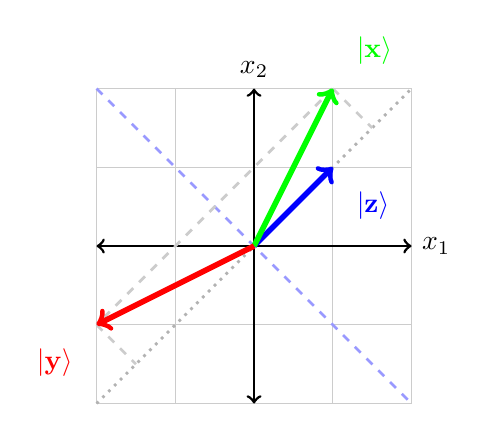
\begin{tikzpicture}  [scale=1]

\tikzstyle{every path}=[line width=1pt]

\newdimen\ms
\ms=0.1cm
\tikzstyle{s1}=[color=red,rectangle,inner sep=3.5]
\tikzstyle{c3}=[circle,inner sep={\ms/8},minimum size=4*\ms]
\tikzstyle{c2}=[circle,inner sep={\ms/8},minimum size=3*\ms]
\tikzstyle{c1}=[circle,inner sep={\ms/8},minimum size=2*\ms]
\tikzstyle{cs1}=[circle,inner sep={\ms/8},minimum size=1*\ms]

% Define positions of all observables


\coordinate (zero) at (0,0);
\coordinate (v) at (1,1);
\coordinate (x) at (1,2);
\coordinate (y) at (-2,-1);

% draw coordinate system

  \draw[thin,gray!40] (-2,-2) grid (2,2);
  \draw[<->] (-2,0)--(2,0) node[right]{$x_1$};
  \draw[<->] (0,-2)--(0,2) node[above]{$x_2$};


% draw vectors

 \draw[dashed, line width=1pt,blue!40](-2,2)--(2,-2);
 \draw[dotted, line width=1pt,gray!60](-2,-2)--(2,2);


 \draw[dashed, line width=1pt,gray!40](x)--(y);
 \draw[dashed, line width=1pt,gray!40](x)--(1.5,1.5);
 \draw[dashed, line width=1pt,gray!40](y)--(-1.5,-1.5);

 \draw[->,line width=2pt,blue](zero)--(v) node[label=below right:{$\vert {\bf z}\rangle $}] {};

 \draw[->,line width=2pt,green](zero)--(x) node[label=above right:{$\vert {\bf x}\rangle $}] {};

 \draw[->,line width=2pt,red](zero)--(y) node[label=below left:{$\vert {\bf y}\rangle $}] {};


\end{tikzpicture}
}
\end{center}
\caption{\label{2021-mm-fdvs-housholder}
Depiction of the Householder transformation $\textsf{\textbf{U}}_{\bf z}$
with
$\vert {\bf z} \rangle =\begin{pmatrix}1,1\end{pmatrix}^\intercal$
acting on a vector $\vert {\bf x} \rangle =\begin{pmatrix}2,1\end{pmatrix}^\intercal$.
The resulting ``reflected'' vector $\vert {\bf y} \rangle = \textsf{\textbf{U}}_{\bf z} \vert {\bf x} \rangle$
and the original vector $\vert {\bf x} \rangle$
have the same length or norm.
Its component along $\vert {\bf z} \rangle$ is reversed, whereas its component orthogonal to
$\vert {\bf z} \rangle$ remains the same.}
\end{marginfigure}
}

Take
 $\vert {\bf x} \rangle =\begin{pmatrix}2,1\end{pmatrix}^\intercal$,
so that
 $\vert {\bf y} \rangle =-\begin{pmatrix}1,2\end{pmatrix}^\intercal$:
this ``reflected'' vector $\vert {\bf y} \rangle$ and the original vector $\vert {\bf x} \rangle$
have the same length or norm.
The component of $\vert {\bf y} \rangle$  along $\vert {\bf z} \rangle$ is reversed, whereas its component orthogonal to
$\vert {\bf z} \rangle$ remains the same.
This situation is depicted in Figure~\ref{2021-mm-fdvs-housholder}.
\eexample
}


As a consequence of (iii), if $\vert {\bf x} \rangle \neq \vert {\bf y} \rangle$ are two vectors  in $\mathbb{R}^n$
with identical length or norm
$\| {\bf x} \| = \| {\bf y} \|$
then there exists a remarkable ``symmetry delivered by'' a Householder transformation $\textsf{\textbf{U}}_{\bf z}$ such that
$\textsf{\textbf{U}}_{\bf z} \vert {\bf x} \rangle =  \vert {\bf y} \rangle$
and
$\textsf{\textbf{U}}_{\bf z}\textsf{\textbf{U}}_{\bf z} \vert {\bf x} \rangle =  \textsf{\textbf{U}}_{\bf z}\vert {\bf y} \rangle
=  \vert {\bf x} \rangle$.
For this to hold the vector $\vert {\bf z} \rangle$ needs to be a  vector equal to $\vert {\bf x} \rangle - \vert {\bf y} \rangle$:
$  \left( \mathbb{1}- 2  ( \langle {\bf z} \vert   {\bf z} \rangle )^{-1} \vert {\bf z} \rangle \langle  {\bf z}  \vert  \right) \vert {\bf x} \rangle =  \vert {\bf y} \rangle
$
and
$ \vert {\bf x} \rangle  =   \left( \mathbb{1}- 2  ( \langle {\bf z} \vert   {\bf z} \rangle )^{-1}\vert {\bf z} \rangle \langle  {\bf z}  \vert  \right) \vert {\bf y} \rangle
$,
resulting in
$( \langle {\bf z} \vert   {\bf z} \rangle )^{-1} \vert {\bf z} \rangle \langle  {\bf z}  \vert  \left( \vert {\bf x} \rangle  - \vert {\bf y} \rangle \right)
= \vert {\bf x} \rangle  - \vert {\bf y} \rangle
$, and thus $\vert {\bf z} \rangle =  \vert {\bf x} \rangle  - \vert {\bf y} \rangle$.
(For $\vert {\bf x} \rangle = \vert {\bf y} \rangle$ identify with $\vert {\bf z} \rangle$ a vector orthogonal to $\vert {\bf x} \rangle = \vert {\bf y} \rangle$.)
This is not true for $\mathbb{C}^n$, as for instance, there exists no $ \vert {\bf z} \rangle $ which would render
$\textsf{\textbf{U}}_{\bf z} \vert {\bf x} \rangle =  i \vert {\bf x} \rangle$ for nonzero  $ \vert {\bf x} \rangle $,
and an additional unitary transformation is required.

This gives rise to the orthonormalizion of a set of $k$ linear independent nonzero vectors
${\frak S}=\{\vert {\bf s}_1\rangle ,
\vert  {\bf s}_2\rangle , \ldots , \vert {\bf s}_k\rangle \}$   in $\mathbb{R}^n$
by taking some orthonormal basis
${\frak B}=\{{\bf e}_1,  {\bf e}_2, \ldots , {\bf e}_n\}\equiv \{\vert {\bf e}_1\rangle ,
\vert  {\bf e}_2\rangle , \ldots , \vert {\bf e}_n\rangle \}$,
choosing $k$ vectors thereof---say, the first $k$ vectors of the standard Cartesian coordinate system---and identifying
$\vert {\bf s}_i\rangle$ with $\vert {\bf x}_i\rangle$,
and (the extra factor $\| {\bf s}_i \|$ serves to make the vector of equal length or norm)
$\vert {\bf y}_i\rangle$ with $\| {\bf s}_i \| \vert {\bf e}_i\rangle$,
thereby constructing a Housholder transformation followed by normalization (through division by $\| {\bf s}_i \|$)
$\textsf{\textbf{U}}_{{\bf z}_i}$ of $\vert {\bf s}_i\rangle \stackrel{\textsf{\textbf{U}}_{{\bf z}_i}}{\mapsto} \vert {\bf e}_i\rangle$
with respective
$\vert {\bf z}_i\rangle = \vert {\bf s}_i\rangle  - \| {\bf s}_i \| \vert {\bf e}_i\rangle$.
This kind of orthonormalization may yield a span ``outside'' of the  subspace  spanned by the ``original'' vectors.

\section{Orthonormal (orthogonal) transformation}
\index{orthonormal transformation}
\index{orthogonal transformation}
\label{2015-m-ch-fdlvs-orthproj}

Orthonormal (orthogonal) transformations are special cases of unitary transformations restricted to {\em real} Hilbert space.

An {\em orthonormal} or {\em orthogonal transformation} $\textsf{\textbf{R}}$ is a linear transformation
whose corresponding square matrix $R$ has real-valued entries
and mutually orthogonal, normalized row (or, equivalently, column) vectors.
As a consequence (see the equivalence of definitions of unitary definitions and the proofs mentioned earlier),
\begin{equation}
\textsf{\textbf{R}}\textsf{\textbf{R}}^\intercal = \textsf{\textbf{R}}^\intercal \textsf{\textbf{R}}= \mathbb{1},
\textrm{ or } \textsf{\textbf{R}}^{-1}=\textsf{\textbf{R}}^\intercal  .
\end{equation}
As all unitary transformations, orthonormal transformations $\textsf{\textbf{R}}$
preserve a symmetric inner product as well as the norm.

If $\textrm{det} \textsf{\textbf{R}}=1$, $\textsf{\textbf{R}}$ corresponds to a {\em rotation.}
\index{rotation}
If $\textrm{det} \textsf{\textbf{R}}=-1$, $\textsf{\textbf{R}}$ corresponds to a rotation and a {\em reflection.}
\index{reflection}
A reflection is an isometry (a distance preserving map) with a hyperplane as set of fixed points.

As a special case of the decomposition~(\ref{2019-ch-fdvs-ditoonb}) of unitary transformations,
orthogonal transformations ave a decomposition
in terms of two orthonormal bases whose elements have real-valued components
${\frak B}=\{{\bf e}_1,  {\bf e}_2, \ldots , {\bf e}_n\}\equiv \{\vert {\bf e}_1\rangle , \vert  {\bf e}_2\rangle , \ldots , \vert {\bf e}_n\rangle \}$
${\frak B}'=\{{\bf f}_1,  {\bf f}_2, \ldots , {\bf f}_n\}\equiv \{\vert {\bf f}_1\rangle , \vert  {\bf f}_2\rangle , \ldots , \vert {\bf f}_n\rangle \}$,
such that
\begin{equation}
\textsf{\textbf{R}}_{ef}= \sum_{i=1}^n  {\bf e}_i {\bf f}_i^\intercal
\equiv \sum_{i=1}^n  \vert {\bf e}_i\rangle \langle {\bf f}_i \vert
.
\label{2019-ch-fdvs-ditoonbr}
\end{equation}

{\color{blue}
\bexample
For the sake of a two-dimensional  example of rotations in the plane ${\Bbb R}^2$,
take the rotation matrix in Equation~(\ref{2012-m-ch-fdvs-otd2})
representing a rotation of the basis by an angle $\varphi$.

\eexample
}


\section{Permutation}
\index{permutation}
\label{2018-permutation}

Permutations are  ``discrete'' orthogonal transformations
``restricted to binary values''
in the sense that
they merely allow the entries ``$0$'' and ``$1$'' in their respective matrix representations.
With regards to classical and quantum bits\cite{mermin-04,mermin-07}
they serve as a sort of ``reversible classical analog'' for classical reversible computation,
as compared to the more general, continuous unitary transformations of quantum bits introduced earlier.

{\color{blue}
\bexample
Permutation matrices are defined by the requirement that they only contain a single nonvanishing entry ``$1$'' per row and column;
all the other row and column entries vanish; that is, the respective matrix entries are ``$0$.''
For example, the matrices $\mathbb{1}_n=\textrm{diag}(\underbrace{1,\ldots ,1}_{n \textrm{ times}})$,
or
\begin{equation}
\sigma_1=
%\left(
\begin{pmatrix}
0&1\\
1&0
\end{pmatrix}
\textrm{, or }\;
%\left(
\begin{pmatrix}
0&1&0\\
1&0&0\\
0&0&1
\end{pmatrix}
\end{equation}
are permutation matrices.
\eexample
}

From the definition and from matrix multiplication follows that,
if $\textsf{\textbf{P}}$ is a permutation represented by its permutation matrix,
then $\textsf{\textbf{P}}\textsf{\textbf{P}}^\intercal =\textsf{\textbf{P}}^\intercal  \textsf{\textbf{P}}=\mathbb{1}_n$.
That is, $\textsf{\textbf{P}}^\intercal $ represents the inverse element of $\textsf{\textbf{P}}$.
As $\textsf{\textbf{P}}$ is real (actually, binary)-valued, it is a {\em normal operator} (cf. page \pageref{2014-m-fdvs-normality}).
\index{normal operator}
\index{normal transformation}


Just as for unitary and orthogonal transformations~(\ref{2019-ch-fdvs-ditoonb})
and~(\ref{2019-ch-fdvs-ditoonbr}),
any permutation matrix can be decomposed as sums of tensor products of row and (dual) column vectors:
The set of all these row and column vectors
with permuted elements:
Suppose
${\frak B}=\{{\bf e}_1,  {\bf e}_2, \ldots , {\bf e}_n\}\equiv \{\vert {\bf e}_1\rangle , \vert  {\bf e}_2\rangle , \ldots , \vert {\bf e}_n\rangle \}$
${\frak B}'=\{{\bf f}_1,  {\bf f}_2, \ldots , {\bf f}_n\}\equiv \{\vert {\bf f}_1\rangle , \vert  {\bf f}_2\rangle , \ldots , \vert {\bf f}_n\rangle \}$,
represent
Cartesian standard basis of $n$-dimensional vector space
and an orthonormal basis whose elements are permutations of elements thereof,
respectively; such that, if $\pi (i)$ stands for the permutation of $i$, ${\bf f}_i = {\bf e}_{\pi (i)}$.
Then
\begin{equation}
\textsf{\textbf{P}}_{ef}= \sum_{i=1}^n  {\bf e}_i {\bf f}_i^\intercal
\equiv \sum_{i=1}^n  \vert {\bf e}_i\rangle \langle {\bf e}_{\pi (i)} \vert
\equiv
\begin{pmatrix}
\langle {\bf e}_{\pi (1)} \vert \\
\langle {\bf e}_{\pi (2)} \vert \\
\vdots \\
\langle {\bf e}_{\pi (n)} \vert \\
\end{pmatrix}
.
\label{2019-ch-fdvs-ditoonbp}
\end{equation}

If $P$ and $Q$ are permutation matrices, so is $PQ$ and $QP$.
The set of all $n!$
permutation $(n\times n)-$matrices corresponding to permutations of $n$ elements of $\{ 1,2,\ldots ,n\}$ form the
{\em symmetric group $S_n$}, with $\mathbb{1}_n$ being the identity element.
\index{symmetric group}


The space spanned the permutation matrices is $\left[(n-1)^2+1\right]$-dimensional;
with $n!>(n-1)^2+1$ for $n>2$.
Therefore,  the bound from above can be improved such that decompositions with $k \le (n-1)^2 +1= n^2-2(n+1)$
exist.\cite[-20mm]{Marcus-Ree-1959}

{\color{blue}
\bexample
For instance, the identity matrix in three dimensions is a permutation
and can be written in terms of the other permutations as
\begin{equation}
\begin{split}
\begin{pmatrix}
1&0&0\\
0&1&0\\
0&0&1
\end{pmatrix}
=
\begin{pmatrix}
1&0&0\\
0&0&1\\
0&1&0
\end{pmatrix}
+
\begin{pmatrix}
0&1&0\\
1&0&0\\
0&0&1
\end{pmatrix}\qquad
\\
-
\begin{pmatrix}
0&1&0\\
0&0&1\\
1&0&0
\end{pmatrix}
-
\begin{pmatrix}
0&0&1\\
1&0&0\\
0&1&0
\end{pmatrix}
+
\begin{pmatrix}
0&0&1\\
0&1&0\\
1&0&0
\end{pmatrix}
.
\end{split}
\end{equation}
\eexample
}

\section{Projection or projection operator}
\label{2011-m-projec}

\index{projection}
\index{projector}
\index{projection operator}

The more I learned about quantum mechanics the more
I realized the importance of projection operators for its conceptualization:\cite[0mm]{v-neumann-49,birkhoff-36}
\begin{itemize}
\item[(i)]
Pure quantum states
\index{pure state}
are represented by a very particular kind of projections;
namely, those that are of the {\em trace class one,} meaning their trace (cf. Section~\ref{2013-ch-fdvs-trace}) is one,
as well as being {\em positive}
(cf. Section~\ref{2015-m-ch-fdlvs-positive}).
Positivity implies
that the projection is {\em self-adjoint} (cf. Section~\ref{2015-m-ch-fdlvs-self-adjoint}),
which is equivalent to the projection being {\em orthogonal}.

{\em Mixed} quantum states
\index{mixed state}
are compositions -- actually, nontrivial convex combinations~\marginnote{For a proof,  see pages 52--53 of~\bibentry{ba-89}.} -- of (pure) quantum states; again they are of the trace class one, self-adjoint, and positive;
yet unlike pure states, they are not projectors (that is, they are not idempotent);
and the trace of their square is not one (indeed, it is less than one).
\item[(ii)]
Mixed states, should they ontologically exist, can be composed of projections by summing over projectors.
\item[(iii)]
Projectors serve as the most elementary observables -- they correspond to yes-no propositions.
\item[(iv)]
In Section~\ref{2012-m-ch-Spectraltheorem} we will learn
that every observable can be decomposed into weighted (spectral) sums of projections.
\item[(v)]
Furthermore, from dimension three onwards, Gleason's theorem (cf. Section~\ref{Gleasontheorem}) allows
quantum probability theory to be based upon maximal (in terms of co-measurability) ``quasi-classical''
blocks of projectors.
\item[(vi)]
Such maximal blocks of projectors can be bundled together to show (cf. Section~\ref{2011-m-KST})
that the corresponding algebraic
structure has no two-valued measure (interpretable as truth assignment), and
therefore cannot be ``embedded'' into a ``larger'' classical (Boolean) algebra.
\end{itemize}



\subsection{Definition}
\marginnote[-15mm]{For proofs and additional information see {\S}41 in~\bibentry{halmos-vs}.}
If ${\frak V}$ is the direct sum of some subspaces
${\frak M}$
and
${\frak N}$
so that every ${\bf z} \in {\frak V}$ can be uniquely written in the form
$
{\bf z}
=
{\bf x}
+
{\bf y}
$, with
${\bf x} \in {\frak M}$
and with
${\bf y} \in {\frak N}$,
then
the {\em projection}, or, used synonymously,
{\em projection operator}
on ${\frak M}$
along ${\frak N}$, is the transformation $\textsf{\textbf{E}}$
defined by $\textsf{\textbf{E}}{\bf z}={\bf x}$.
Conversely,
 $\textsf{\textbf{F}}{\bf z}={\bf y}$  is the projection
on ${\frak N}$
along ${\frak M}$.

A (nonzero) linear transformation $\textsf{\textbf{E}}$ is a {\em projector}
\index{projector}
if and only if one of
the following conditions is satisfied (then all the others are also satisfied):\cite{Trenkler1994}
\begin{itemize}
\item[(i)]
$\textsf{\textbf{E}}$ is idempotent; that is,
\index{idempotence}
$\textsf{\textbf{E}}\textsf{\textbf{E}}=\textsf{\textbf{E}}\neq 0$;

\item[(ii)]
$\textsf{\textbf{E}}^k$ is a projector for all $k \in \mathbb{N}$;

\item[(iii)]
$\textsf{\textbf{1}}-\textsf{\textbf{E}}$ is the {\em complimentary projection} with respect to $\textsf{\textbf{E}}$:
if $\textsf{\textbf{E}}$  is the projection
on ${\frak M}$
along ${\frak N}$,
 $\textsf{\textbf{1}}-\textsf{\textbf{E}}$ is the projection
on ${\frak N}$
along ${\frak M}$; in particular, $\left(\textsf{\textbf{1}}-\textsf{\textbf{E}}\right)\textsf{\textbf{E}}=\textsf{\textbf{E}}-\textsf{\textbf{E}}^2=\textsf{\textbf{E}}-\textsf{\textbf{E}}=0$.

\item[(iv)]
$\textsf{\textbf{E}}^\intercal$ is a projector;

\item[(v)]
$\textsf{\textbf{A}}= 2\textsf{\textbf{E}} - \textsf{\textbf{1}}$ is an involution;
that is, $\textsf{\textbf{A}}^2 = \mathbb{1}=\textsf{\textbf{1}}$;
\index{involution}
see also Section~\ref{2021-m-ch-hposholder} on Householder transformations;
\index{Householder transformation}

\item[(vi)]
$\textsf{\textbf{E}}$ admits the representation
\marginnote{See {\S}~5.8, Corollary~1 in~\bibentry{Lancaster-Tismenetsky}.}
\begin{equation}
\textsf{\textbf{E}} =\sum_{i=1}^k {\bf x}_i {\bf y}_i^\ast,
\label{2018-mm-ch-fdlvs-dop}
\end{equation}
where $k$ is the rank of $\textsf{\textbf{E}}$ and
$\{ {\bf x}_1, \ldots ,{\bf x}_k\}$
and
$\{ {\bf y}_1, \ldots ,{\bf y}_k\}$
are {\em biorthogonal} systems of vectors (not necessarily bases) of the vector space
\index{biorthogonality}
such that ${\bf y}_i^\ast  {\bf x}_j \equiv \langle {\bf y}_i \vert {\bf x}_j \rangle = \delta_{ij}$.
If the systems of vectors are identical; that is, if ${\bf y}_i={\bf x}_i$,
the products $ {\bf x}_i {\bf x}_i^\ast   \equiv \vert {\bf x}_i\rangle \langle {\bf x}_i \vert$ project onto one-dimensional subspaces
spanned by ${\bf x}_i$, and the projection is self-adjoint, and thus orthogonal.



\end{itemize}

{\color{OliveGreen}
\bproof
For a proof of (i) note that, if $\textsf{\textbf{E}}$  is the projection
on ${\frak M}$
along ${\frak N}$,
and if
$
{\bf z}
=
{\bf x}
+
{\bf y}
$, with
${\bf x} \in {\frak M}$
and with
${\bf y} \in {\frak N}$,
the decomposition of ${\bf x}$ yields
${\bf x}+0$, so that
$\textsf{\textbf{E}}^2{\bf z}=\textsf{\textbf{E}}\textsf{\textbf{E}}{\bf z}=\textsf{\textbf{E}}{\bf x}
={\bf x}=\textsf{\textbf{E}}{\bf z}$.
The converse --
idempotence
``$\textsf{\textbf{E}}\textsf{\textbf{E}}=\textsf{\textbf{E}}$''
implies that $\textsf{\textbf{E}}$ is a projection -- is more difficult to prove.


For the necessity of (iii) note that $(\textsf{\textbf{1}}-\textsf{\textbf{E}})^2
=\textsf{\textbf{1}}-\textsf{\textbf{E}}-\textsf{\textbf{E}}+ \textsf{\textbf{E}}^2
=\textsf{\textbf{1}}-\textsf{\textbf{E}}$;
furthermore,
$
\textsf{\textbf{E}}(\textsf{\textbf{1}}-\textsf{\textbf{E}})=
(\textsf{\textbf{1}}-\textsf{\textbf{E}})\textsf{\textbf{E}}=
\textsf{\textbf{E}}- \textsf{\textbf{E}}^2=0
$.

\eproof
}



\marginnote{The vector norm (\ref{2018-mm-ch-vn}) on page~\pageref{2018-mm-ch-vn} induces an operator norm
by $\| \textsf{\textbf{A}} \| = \sup_{\| {\bf x} \| =1} \| \textsf{\textbf{A}} {\bf x} \|$.}
We state without proof\cite{Szyld2006} that, for all projections
which are neither null nor the identity,
\index{norm}
the norm of its complementary projection
is identical with the norm of the projection; that is,
\begin{equation}
\left\| \textsf{\textbf{E}} \right\| = \left\| \textsf{\textbf{1}} - \textsf{\textbf{E}} \right\|
.
\end{equation}




%\subsection{Combination of projections}




\subsection{Orthogonal (perpendicular) projections}
\index{orthogonal projection}
\index{perpendicular projection}
\marginnote{For proofs and additional information see {\S}42, {\S}75 \& {\S}76 in~\bibentry{halmos-vs}.}

{\em Orthogonal,} or, used synonymously,
{\em perpendicular} projections
are associated with a {\em direct sum decomposition} of the vector space ${\frak V}$;
that is,
\begin{equation}
 {\frak M}\oplus {\frak M}^\perp ={\frak V},
\label{2012-m-ch-fdvs-perp}
\end{equation}
whereby $ {\frak M}= P_{\frak M}({\frak V})$
is the image of some projector $\textsf{\textbf{E}}=P_{\frak M}$
along ${\frak M}^\perp$, and  ${\frak M}^\perp$ is
the kernel of $P_{\frak M}$.
That is, ${\frak M}^\perp = \left\{{\bf x} \in {\frak V} \mid P_{\frak M}({\bf x}) = {\bf 0}\right\}$
\index{kernel}
is the subspace of ${\frak V}$
whose elements are mapped to the zero vector ${\bf 0}$ by $P_{\frak M}$.


Let us, for the sake of concreteness,
\marginnote{\url{http://faculty.uml.edu/dklain/projections.pdf}}
suppose that, in $n$-dimensional complex Hilbert space
${\Bbb C}^n$, we are given a $k$-dimensional subspace
\begin{equation}
{\frak M} = \textrm{span}\left( {\bf x}_1,\ldots ,{\bf x}_k \right)
\equiv \textrm{span}\left(\vert {\bf x}_1\rangle ,\ldots ,\vert {\bf x}_k \right\rangle )
\end{equation}
spanned
\index{linear span}
\index{span}
by  $k \le n$  linear independent base vectors ${\bf x}_1,\ldots ,{\bf x}_k$.
In addition, we are given another (arbitrary) vector ${\bf y} \in {\Bbb C}^n$.

Now consider the following question:
how can we project ${\bf y}$ onto ${\frak M}$ orthogonally (perpendicularly)?
That is, can we find a vector ${\bf y}' \in {\frak M}$ so that ${\bf y}^\perp = {\bf y} - {\bf y}'$
is orthogonal (perpendicular) to all of ${\frak M}$?

The orthogonality of ${\bf y}^\perp$ on the entire ${\frak M}$ can be rephrased in terms
of all the vectors ${\bf x}_1,\ldots ,{\bf x}_k$ spanning ${\frak M}$; that is,
for all ${\bf x}_i \in {\frak M}$, $1\le i\le k$
we must have
$\langle {\bf x}_i \vert {\bf y}^\perp \rangle = 0$.
This can be transformed into matrix algebra by considering the $n \times k$ matrix
[note that ${\bf x}_i$ are column vectors,
and recall the construction in Equation~(\ref{2015-m-ch-fdlvs-uniascolv})]
\begin{equation}
\textsf{\textbf{A}} = \begin{pmatrix}
{\bf x}_1, \ldots ,{\bf x}_k
\end{pmatrix}
\equiv
\begin{pmatrix}
\vert {\bf x}_1\rangle , \ldots , \vert {\bf x}_k \rangle
\end{pmatrix},
\end{equation}
and by requiring
\begin{equation}
\textsf{\textbf{A}}^\dagger \vert {\bf y}^\perp \rangle   \equiv
 \textsf{\textbf{A}}^\dagger  {{\bf y}^\perp} =
 \textsf{\textbf{A}}^\dagger  \left({\bf y} - {\bf y}'\right) =
 \textsf{\textbf{A}}^\dagger {\bf y}  - \textsf{\textbf{A}}^\dagger {{\bf y}'}   =
0,
\end{equation}
yielding
\begin{equation}
 \textsf{\textbf{A}}^\dagger  \vert  {\bf y}  \rangle
\equiv
 \textsf{\textbf{A}}^\dagger   {\bf y}
=
\textsf{\textbf{A}}^\dagger  {{\bf y}'}
\equiv
\textsf{\textbf{A}}^\dagger \vert {\bf y}' \rangle .
\label{2015-m-ch-cfvs-opab1}
\end{equation}

On the other hand, ${\bf y}'$ must be a linear combination of
${\bf x}_1,\ldots ,{\bf x}_k$ with the $k$-tuple of coefficients ${\bf c}$ defined by
\marginnote{Recall that
$(\textsf{\textbf{A}}\textsf{\textbf{B}})^\dagger =\textsf{\textbf{B}}^\dagger \textsf{\textbf{A}}^\dagger $,
and $(\textsf{\textbf{A}}^\dagger )^\dagger =\textsf{\textbf{A}}$.}
\begin{equation}
{\bf y}'
=
c_1 {\bf x}_1 + \cdots + c_k {\bf x}_k
=
\begin{pmatrix}{\bf x}_1, \ldots ,{\bf x}_k
\end{pmatrix}
\begin{pmatrix} c_1\\ \vdots \\ c_k
\end{pmatrix}
=
\textsf{\textbf{A}}  {\bf c}
.
\label{2015-m-ch-cfvs-opab22}
\end{equation}
Insertion into (\ref{2015-m-ch-cfvs-opab1}) yields
\begin{equation}
\textsf{\textbf{A}}^\dagger  {\bf y}
=
\textsf{\textbf{A}}^\dagger  \textsf{\textbf{A}} {\bf c}
.
\label{2015-m-ch-cfvs-opab2}
\end{equation}
Taking the inverse of $\textsf{\textbf{A}}^\dagger  \textsf{\textbf{A}} $
(this is a $k \times k$ diagonal matrix which is invertible, since
the $k$ vectors defining $\textsf{\textbf{A}}$ are linear independent),
and multiplying (\ref{2015-m-ch-cfvs-opab2}) from the left yields
\begin{equation}
{\bf c}
=
\left(\textsf{\textbf{A}}^\dagger  \textsf{\textbf{A}} \right)^{-1} \textsf{\textbf{A}}^\dagger {\bf y}
.
\label{2015-m-ch-cfvs-opab3}
\end{equation}
With (\ref{2015-m-ch-cfvs-opab22}) and (\ref{2015-m-ch-cfvs-opab3})
we find ${\bf y}'$ to be
\begin{equation}
{\bf y}'
=
\textsf{\textbf{A}}  {\bf c} =
\textsf{\textbf{A}}  \left(\textsf{\textbf{A}}^\dagger  \textsf{\textbf{A}} \right)^{-1} \textsf{\textbf{A}}^\dagger {\bf y}
.
\label{2015-m-ch-cfvs-opab4}
\end{equation}
We can define
\begin{equation}
\textsf{\textbf{E}}_{{\frak M}}=
\textsf{\textbf{A}}  \left(\textsf{\textbf{A}}^\dagger  \textsf{\textbf{A}} \right)^{-1} \textsf{\textbf{A}}^\dagger
\label{2015-m-ch-cfvs-opab5}
\end{equation}
to be the {\em projection matrix for the subspace ${\frak M}$}.
Note that
\begin{equation}
\begin{split}
\textsf{\textbf{E}}_{{\frak M}}^\dagger
=
\left[
\textsf{\textbf{A}}  \left(\textsf{\textbf{A}}^\dagger
\textsf{\textbf{A}} \right)^{-1} \textsf{\textbf{A}}^\dagger
\right]^\dagger
=
\textsf{\textbf{A}} \left[  \left(\textsf{\textbf{A}}^\dagger
\textsf{\textbf{A}} \right)^{-1}\right]^\dagger \textsf{\textbf{A}}^\dagger
=
\textsf{\textbf{A}} \left[ \textsf{\textbf{A}}^{-1}
\left(\textsf{\textbf{A}}^\dagger\right)^{-1} \right]^\dagger \textsf{\textbf{A}}^\dagger \\
=
\textsf{\textbf{A}} \textsf{\textbf{A}}^{-1}
\left(\textsf{\textbf{A}}^{-1}\right)^\dagger  \textsf{\textbf{A}}^\dagger
= \textsf{\textbf{A}} \textsf{\textbf{A}}^{-1}
\left(\textsf{\textbf{A}}^\dagger\right)^{-1}  \textsf{\textbf{A}}^\dagger
= \textsf{\textbf{A}} \left(\textsf{\textbf{A}}^\dagger
\textsf{\textbf{A}}\right)^{-1}  \textsf{\textbf{A}}^\dagger
=  \textsf{\textbf{E}}_{{\frak M}},
\end{split}
\label{2015-m-ch-cfvs-opab6}
\end{equation}
that is, $\textsf{\textbf{E}}_{{\frak M}}$ is self-adjoint and thus normal, as well as idempotent:
\begin{equation}
\begin{split}
\textsf{\textbf{E}}_{{\frak M}}^2
=
\left(
\textsf{\textbf{A}}  \left(\textsf{\textbf{A}}^\dagger
\textsf{\textbf{A}} \right)^{-1} \textsf{\textbf{A}}^\dagger
\right)
\left(
\textsf{\textbf{A}}  \left(\textsf{\textbf{A}}^\dagger
\textsf{\textbf{A}} \right)^{-1} \textsf{\textbf{A}}^\dagger
\right) \\
=
\textsf{\textbf{A}}^\dagger  \left(\textsf{\textbf{A}}^\dagger
\textsf{\textbf{A}} \right)^{-1} \left( \textsf{\textbf{A}}^\dagger
\textsf{\textbf{A}}  \right) \left(\textsf{\textbf{A}} ^\dagger
\textsf{\textbf{A}} \right)^{-1} \textsf{\textbf{A}}
=
\textsf{\textbf{A}}^\dagger   \left(\textsf{\textbf{A}} ^\dagger
\textsf{\textbf{A}} \right)^{-1} \textsf{\textbf{A}}
=
\textsf{\textbf{E}}_{{\frak M}}.
\end{split}
\label{2015-m-ch-cfvs-opab7}
\end{equation}

Conversely, every normal projection operator has a ``trivial'' spectral decomposition
(cf. Section~\ref{2012-m-ch-Spectraltheorem} on page \pageref{2012-m-ch-Spectraltheorem})
$\textsf{\textbf{E}}_{{\frak M}}
=
1 \cdot \textsf{\textbf{E}}_{{\frak M}} + 0 \cdot \textsf{\textbf{E}}_{{\frak M}^\perp}
=
1 \cdot \textsf{\textbf{E}}_{{\frak M}} + 0 \cdot \left(\textbf{1} - \textsf{\textbf{E}}_{{\frak M}}\right)$
associated with the two eigenvalues $0$ and $1$, and thus must be orthogonal.

If the basis ${\frak B}= \left\{{\bf x}_1,\ldots ,{\bf x}_k \right\}$ of ${\frak M}$
is orthonormal, then
\begin{equation}
\begin{split}
\textsf{\textbf{A}}^\dagger
\textsf{\textbf{A}}
\equiv
\begin{pmatrix}
\langle {\bf x}_1 \vert \\ \vdots \\ \langle {\bf x}_k \vert
\end{pmatrix}
\begin{pmatrix}
\vert {\bf x}_1\rangle , \ldots , \vert {\bf x}_k \rangle
\end{pmatrix}
=
\begin{pmatrix}
\langle {\bf x}_1 \vert {\bf x}_1\rangle   & \ldots &    \langle {\bf x}_1 \vert {\bf x}_k\rangle \\
\vdots &  \vdots &   \vdots \\
\langle {\bf x}_k \vert {\bf x}_1\rangle   & \ldots &    \langle {\bf x}_k \vert {\bf x}_k\rangle \\
\end{pmatrix}
\equiv
\mathbb{1}_k
\end{split}
\end{equation}
represents a $k$-dimensional resolution of the identity operator.
\index{resolution of the identity}
Thus, $\left(\textsf{\textbf{A}}^\dagger  \textsf{\textbf{A}} \right)^{-1}\equiv \left(\mathbb{1}_k\right)^{-1}$
is also a $k$-dimensional resolution of the identity operator,
and the orthogonal projector $\textsf{\textbf{E}}_{{\frak M}}$
in Equation~(\ref{2015-m-ch-cfvs-opab5})
reduces to
\begin{equation}
\textsf{\textbf{E}}_{{\frak M}}=
\textsf{\textbf{A}}   \textsf{\textbf{A}}^\dagger
\equiv
\sum_{i=1}^k \vert {\bf x}_i \rangle \langle {\bf x}_i \vert
.
\end{equation}



{\color{blue}
\bexample
The simplest example of an orthogonal projection onto a one-dimensional subspace of a Hilbert space
spanned by some unit vector $\vert {\bf x} \rangle$ is the dyadic or outer product
$
\textsf{\textbf{E}}_x = \vert {\bf x} \rangle  \langle {\bf x} \vert$.

If two unit vectors $\vert {\bf x} \rangle$ and $\vert {\bf y} \rangle$ are orthogonal;
that is, if $\langle {\bf x} \vert {\bf y} \rangle = 0$, then
$\textsf{\textbf{E}}_{x,y} = \vert {\bf x} \rangle  \langle {\bf x} \vert  +  \vert {\bf y} \rangle  \langle {\bf y} \vert$
is an orthogonal projector onto a two-dimensional subspace spanned by $\vert {\bf x} \rangle$ and $\vert {\bf y} \rangle$.
\eexample
}

In general, the orthonormal projection corresponding to some arbitrary subspace of some Hilbert space can be (nonuniquely)
constructed by
(i) finding an orthonormal basis spanning that subsystem (this is nonunique),
if necessary by a Gram-Schmidt process;
\index{Gram-Schmidt process}
(ii) forming the projection operators corresponding to the dyadic or outer product
\index{dyadic product}
\index{outer product}
of all these vectors; and
(iii) summing up all these orthogonal operators.


The following propositions are stated mostly without proof.
A  linear transformation $\textsf{\textbf{E}}$ is an orthogonal (perpendicular) projection
if and only if is self-adjoint; that is,
$\textsf{\textbf{E}} = \textsf{\textbf{E}}^2=\textsf{\textbf{E}}^\ast $.

Perpendicular projections are {\em positive} linear transformations,
with
$\left\| \textsf{\textbf{E}}{\bf x} \right\| \le \| {\bf x} \|$
for all
${\bf x} \in {\frak V}$.
Conversely,
if a linear transformation $\textsf{\textbf{E}}$
is idempotent; that is,
$\textsf{\textbf{E}}^2=\textsf{\textbf{E}}$,
and  $\left\| \textsf{\textbf{E}}{\bf x} \right\| \le \| {\bf x} \|$
for all
${\bf x} \in {\frak V}$,
then  is self-adjoint; that is,
$\textsf{\textbf{E}}=\textsf{\textbf{E}}^\ast$.

Recall that
for {\em real} inner product spaces, the self-adjoint operator can be identified with a {\em symmetric} operator
$\textsf{\textbf{E}}=\textsf{\textbf{E}}^\intercal $,
\index{symmetric operator}
whereas
for {\em complex} inner product spaces, the self-adjoint operator can be identified with a {\em Hermitian} operator
$\textsf{\textbf{E}}=\textsf{\textbf{E}}^\dagger$.
\index{Hermitian operator}


If $\textsf{\textbf{E}}_1,\textsf{\textbf{E}}_2, \ldots , \textsf{\textbf{E}}_n$ are (perpendicular)
projections,
then a necessary and sufficient condition that
$\textsf{\textbf{E}} =\textsf{\textbf{E}}_1+\textsf{\textbf{E}}_2+\cdots +\textsf{\textbf{E}}_n$
be a (perpendicular) projection is that
 $\textsf{\textbf{E}}_i \textsf{\textbf{E}}_j =\delta_{ij}\textsf{\textbf{E}}_i =\delta_{ij}\textsf{\textbf{E}}_j$;
and, in particular,
$\textsf{\textbf{E}}_i \textsf{\textbf{E}}_j =0$
whenever $i\neq j$; that is, that all $E_i$ are pairwise orthogonal.

{\color{OliveGreen}\bproof
For a start, consider just two projections
 $\textsf{\textbf{E}}_1$ and $\textsf{\textbf{E}}_2$.
Then we can assert that   $\textsf{\textbf{E}}_1 + \textsf{\textbf{E}}_2$ is a projection if and only if
 $\textsf{\textbf{E}}_1 \textsf{\textbf{E}}_2=\textsf{\textbf{E}}_2 \textsf{\textbf{E}}_1=0$.

Because, for
 $\textsf{\textbf{E}}_1 + \textsf{\textbf{E}}_2$ to be a projection, it must be idempotent; that is,
\index{idempotence}
 \begin{equation}
(\textsf{\textbf{E}}_1 + \textsf{\textbf{E}}_2)^2 =
(\textsf{\textbf{E}}_1 + \textsf{\textbf{E}}_2)(\textsf{\textbf{E}}_1 + \textsf{\textbf{E}}_2)  =
\textsf{\textbf{E}}_1^2 +   \textsf{\textbf{E}}_1\textsf{\textbf{E}}_2 + \textsf{\textbf{E}}_2\textsf{\textbf{E}}_1 + \textsf{\textbf{E}}_2^2
=
 \textsf{\textbf{E}}_1 + \textsf{\textbf{E}}_2 .
\label{2012-m-ch-fdvs-pr3}
\end{equation}
As a consequence, the cross-product terms in (\ref{2012-m-ch-fdvs-pr3}) must vanish; that is,
\begin{equation}
\textsf{\textbf{E}}_1\textsf{\textbf{E}}_2 + \textsf{\textbf{E}}_2\textsf{\textbf{E}}_1 =0.
\label{2012-m-ch-fdvs-pr4}
\end{equation}
Multiplication of (\ref{2012-m-ch-fdvs-pr4}) with $\textsf{\textbf{E}}_1$ from the left and from the right yields
\begin{equation}
\begin{split}
\textsf{\textbf{E}}_1\textsf{\textbf{E}}_1\textsf{\textbf{E}}_2 + \textsf{\textbf{E}}_1\textsf{\textbf{E}}_2\textsf{\textbf{E}}_1 =0, \\
 \textsf{\textbf{E}}_1\textsf{\textbf{E}}_2 + \textsf{\textbf{E}}_1\textsf{\textbf{E}}_2\textsf{\textbf{E}}_1 =0;\textrm{ and} \\
\textsf{\textbf{E}}_1\textsf{\textbf{E}}_2\textsf{\textbf{E}}_1 + \textsf{\textbf{E}}_2\textsf{\textbf{E}}_1\textsf{\textbf{E}}_1 =0, \\
\textsf{\textbf{E}}_1\textsf{\textbf{E}}_2\textsf{\textbf{E}}_1 + \textsf{\textbf{E}}_2\textsf{\textbf{E}}_1  =0.
\end{split}
\label{2012-m-ch-fdvs-pr5}
\end{equation}
Subtraction of the resulting pair of equations yields
\begin{equation}
 \textsf{\textbf{E}}_1\textsf{\textbf{E}}_2 - \textsf{\textbf{E}}_2\textsf{\textbf{E}}_1  =
\left[ \textsf{\textbf{E}}_1,\textsf{\textbf{E}}_2 \right]
=0,
\label{2012-m-ch-fdvs-pr6}
\end{equation}
or
\begin{equation}
 \textsf{\textbf{E}}_1\textsf{\textbf{E}}_2 = \textsf{\textbf{E}}_2\textsf{\textbf{E}}_1 .
\label{2012-m-ch-fdvs-pr67}
\end{equation}
Hence, in order for the cross-product terms in Eqs. (\ref{2012-m-ch-fdvs-pr3} ) and (\ref{2012-m-ch-fdvs-pr4})
to vanish, we must have
\begin{equation}
 \textsf{\textbf{E}}_1\textsf{\textbf{E}}_2 = \textsf{\textbf{E}}_2\textsf{\textbf{E}}_1 =0.
\label{2012-m-ch-fdvs-pr8}
\end{equation}

Proving the reverse statement is straightforward, since (\ref{2012-m-ch-fdvs-pr8}) implies  (\ref{2012-m-ch-fdvs-pr3}).

A generalisation by induction to more than two projections is straightforward,
since, for instance,
$\left(\textsf{\textbf{E}}_1+\textsf{\textbf{E}}_2\right)\textsf{\textbf{E}}_3=0$
implies
$ \textsf{\textbf{E}}_1\textsf{\textbf{E}}_3+\textsf{\textbf{E}}_2\textsf{\textbf{E}}_3=0$.
Multiplication with $\textsf{\textbf{E}}_1$ from the left yields
$
\textsf{\textbf{E}}_1\textsf{\textbf{E}}_1\textsf{\textbf{E}}_3+\textsf{\textbf{E}}_1\textsf{\textbf{E}}_2\textsf{\textbf{E}}_3=
\textsf{\textbf{E}}_1 \textsf{\textbf{E}}_3=
0$.
 \eproof }


\subsection{Construction of orthogonal projections from  single unit vectors}

How can we construct  orthogonal projections from unit vectors or systems of orthogonal projections from some vector in some orthonormal basis
with the standard dot product?

Let ${\bf x}$ be the coordinates of a unit vector;
that is $\|{\bf x} \| =1$.
Transposition is indicated by the superscript ``$\intercal$''
in real vector space.
In complex vector space, the transposition has to be substituted
 for the {\em conjugate transpose} (also denoted as
{\em Hermitian conjugate} or {\em Hermitian adjoint}),
\index{conjugate transpose}
\index{Hermitian conjugate}
\index{Hermitian adjoint}
``$\dagger$,'' standing for transposition and complex conjugation of the coordinates.
More explicitly,
\begin{equation}
\begin{split}
\begin{pmatrix}x_1,\ldots, x_n\end{pmatrix}^\dagger =
%\left(
\begin{pmatrix}
\overline{x_1}\\ \vdots\\ \overline{x_n}
\end{pmatrix}
,  \textrm{ and }
%\left(
\begin{pmatrix}
x_1\\ \vdots\\ x_n
\end{pmatrix}^\dagger
= (\overline{x_1},\ldots, \overline{x_n})
.
\end{split}
\end{equation}
Note that, just as for real vector spaces,
$\left({\bf x}^\intercal \right)^\intercal ={\bf x}$,
or, in the bra-ket notation,
$\left(\vert {\bf x}\rangle^\intercal \right)^\intercal =\vert {\bf x}\rangle$,
 so is
$\left({\bf x}^\dagger \right)^\dagger={\bf x}$,
or
$\left(\vert  {\bf x}\rangle ^\dagger \right)^\dagger= \vert{\bf x} \rangle$ for complex vector spaces.

As already mentioned on page~\pageref{2015-m-ch-fdlvs-inter}, Equation~(\ref{2015-m-ch-fdlvs-inter}), for orthonormal bases of complex Hilbert space
we can express the dual vector in terms of the original vector by
taking the conjugate transpose, and {\em vice versa}; that is,
\begin{equation}
\begin{split}
\langle {\bf x} \vert = \left(\vert {\bf x}\rangle \right)^\dagger,
\textrm{ and }
\vert {\bf x}\rangle  = \left(\langle {\bf x}\vert\right)^\dagger.
\end{split}
\end{equation}

In real vector space, the {\em dyadic product}, or {\em tensor product}, or {\em outer product}
\index{outer product}
\index{dyadic product}
\index{tensor product}
\begin{equation}
\begin{split}
\textsf{\textbf{E}}_{\bf x} = {\bf x} \otimes {\bf x}^\intercal  = \vert{\bf x}\rangle \langle {\bf x}\vert
\equiv
\begin{pmatrix}
x_1\\
x_2\\
\vdots \\
x_n
\end{pmatrix}
\begin{pmatrix}x_1,x_2,\ldots ,x_n\end{pmatrix}\\
\\
=
\begin{pmatrix}
x_1\begin{pmatrix}x_1,x_2,\ldots ,x_n\end{pmatrix}\\
x_2\begin{pmatrix}x_1,x_2,\ldots ,x_n\end{pmatrix}\\
\vdots  \\
x_n\begin{pmatrix}x_1,x_2,\ldots ,x_n \end{pmatrix}
\end{pmatrix}
=
\begin{pmatrix}
x_1x_1&x_1x_2& \cdots&x_1x_n\\
x_2x_1&x_2x_2& \cdots&x_2x_n\\
\vdots & \vdots & \vdots &\vdots \\
x_nx_1&x_nx_2& \cdots&x_nx_n
\end{pmatrix}
\end{split}
\end{equation}
is the projection
associated with ${\bf x}$.

If the vector ${\bf x}$ is not normalized,
then the associated projection is
\begin{equation}
\textsf{\textbf{E}}_{\bf x} \equiv \frac{{\bf x} \otimes {\bf x}^\intercal }{\langle {\bf x}\mid {\bf x}\rangle}
\equiv \frac{\vert{\bf x}\rangle \langle {\bf x}\vert}{\langle {\bf x}\mid {\bf x}\rangle}
= \frac{\vert{\bf x}\rangle \langle {\bf x}\vert}{\| {\bf x}\|^2}
\end{equation}
This construction is related to
$P_{\bf x}$ on page \pageref{2011-m-gsp}
by $P_{\bf x}({\bf y})=\textsf{\textbf{E}}_{\bf x}{\bf y}$.

{\color{OliveGreen}
\bproof
For a proof,  consider only normalized vectors ${\bf x}$, and
let $\textsf{\textbf{E}}_{\bf x} = {\bf x}\otimes {\bf x}^\intercal  $,
then
$$
\textsf{\textbf{E}}_{\bf x}\textsf{\textbf{E}}_{\bf x}
=
(\vert{\bf x}\rangle \langle {\bf x}\vert)
(\vert{\bf x}\rangle \langle {\bf x}\vert)
=
\vert{\bf x}\rangle \underbrace{\langle {\bf x}\vert {\bf x}\rangle}_{=1} \langle {\bf x}\vert
=  \textsf{\textbf{E}}_{\bf x}.
$$
More explicitly, by writing out the coordinate tuples, the equivalent proof is
\begin{equation}
\begin{split}
\textsf{\textbf{E}}_{\bf x}\textsf{\textbf{E}}_{\bf x}
\equiv ({\bf x}\otimes {\bf x}^\intercal  ) \cdot ({\bf x}\otimes {\bf x}^\intercal  )
\\
\equiv
\left[
\begin{pmatrix}
x_1\\
x_2\\
\vdots \\
x_n
\end{pmatrix}
(x_1,x_2,\ldots ,x_n)
\right]
\left[
\begin{pmatrix}
x_1\\
x_2\\
\vdots \\
x_n
\end{pmatrix}
(x_1,x_2,\ldots ,x_n)
 \right]
\\
=
\begin{pmatrix}
x_1\\
x_2\\
\vdots \\
x_n
\end{pmatrix}
\underbrace{\left[ (x_1,x_2,\ldots ,x_n)
\begin{pmatrix}
x_1\\
x_2\\
\vdots \\
x_n
\end{pmatrix}
\right]}_{=1}
(x_1,x_2,\ldots ,x_n)
\equiv\textsf{\textbf{E}}_{\bf x}. \textrm{\eproof }
\end{split}
\end{equation}
}

In complex vector space, transposition has to be substituted by the conjugate transposition;
\index{conjugate transpose}
\index{Hermitian conjugate}
\index{Hermitian adjoint}
that is
\begin{equation}
\begin{split}
\textsf{\textbf{E}}_{\bf x} = {\bf x} \otimes {\bf x}^\dagger \equiv \vert{\bf x}\rangle \langle {\bf x}\vert
\end{split}
\end{equation}

{
\color{blue}
\bexample
For two examples, let
${\bf x}=(1,0)^\intercal $
and
${\bf y}=(1,-1)^\intercal $;
then
$$
\textsf{\textbf{E}}_{\bf x}
=
\begin{pmatrix}
1\\
0
\end{pmatrix}
(1,0)
=
\begin{pmatrix}
1(1,0)\\
0(1,0)
\end{pmatrix}
=
\begin{pmatrix}
1&0\\
0&0
\end{pmatrix}
,
$$
and
$$
\textsf{\textbf{E}}_{\bf y}
= \frac{1}{2}
\begin{pmatrix}
1\\
-1
\end{pmatrix}
(1,-1)
= \frac{1}{2}
\begin{pmatrix}
1(1,-1)\\
-1(1,-1)
\end{pmatrix}
= \frac{1}{2}
\begin{pmatrix}
1&-1\\
-1&1
\end{pmatrix}
.
\textrm{\eexample}
$$
%\eexample
}

Note also that
\begin{equation}
\textsf{\textbf{E}}_{\bf x} \vert {\bf y}\rangle
\equiv
\textsf{\textbf{E}}_{\bf x} {\bf y}
=
\langle {\bf x}\vert  {\bf y} \rangle {\bf x},
\equiv
\langle {\bf x}\vert  {\bf y} \rangle \vert {\bf x}\rangle ,
\end{equation}
which can be directly proven by insertion.





\subsection{Examples of oblique projections which are not orthogonal projections}

{\color{blue}
\bexample

Examples for projections which are not orthogonal are
$$\begin{pmatrix}
1&\alpha \\
0&0
\end{pmatrix}
\text{,  or }
\begin{pmatrix}
1&0&\alpha \\
0&1&\beta \\
0&0&0
\end{pmatrix},$$
with $\alpha \neq 0$.
Such projectors are sometimes called
{\em oblique} projections.
\index{oblique projections}



For two-dimensional Hilbert space, the solution
of idempotence
%Reduce[{{a, b}, {c, d}}.{{a, b}, {c, d}} == {{a, b}, {c, d}}, {a, b,  c, d}]
$$
\begin{pmatrix}
a&b \\
c&d
\end{pmatrix}
\begin{pmatrix}
a&b \\
c&d
\end{pmatrix}
=
\begin{pmatrix}
a&b \\
c&d
\end{pmatrix}
$$
yields the three orthogonal projections
$$
\begin{pmatrix}
1&0 \\
0&0
\end{pmatrix},
\begin{pmatrix}
0&0 \\
0&1
\end{pmatrix},\text{ and }
\begin{pmatrix}
1&0 \\
0&1
\end{pmatrix},
$$
as well as a continuum of oblique projections
$$
\begin{pmatrix}
0&0 \\
c&1
\end{pmatrix}
=
\begin{pmatrix}
0 \\
1
\end{pmatrix}
\otimes
\begin{pmatrix}
c,1
\end{pmatrix},
\begin{pmatrix}
1&0 \\
c&0
\end{pmatrix},\text{ and }
\begin{pmatrix}
a&b \\
\frac{a(1-a)}{b}&1-a
\end{pmatrix},
$$
with $a,b,c \neq 0$.

$$
\begin{pmatrix}
0&0 \\
c&1
\end{pmatrix}
=
\begin{pmatrix}
0 \\
1
\end{pmatrix}
\otimes
\begin{pmatrix}
c,1
\end{pmatrix},
\begin{pmatrix}
1&0 \\
c&0
\end{pmatrix}
$$

One can also utilize Equation~(\ref{2018-mm-ch-fdlvs-dop}) and
define two sets of indexed vectors
$\{ {\bf e}_1 , {\bf e}_2 \}$ and
$\{ {\bf f}_1 , {\bf f}_2 \}$
with
$ {\bf e}_1 \equiv \vert {\bf e}_1\rangle =\begin{pmatrix} a,b\end{pmatrix}^\intercal$,
$ {\bf e}_2 \equiv \vert {\bf e}_2\rangle =\begin{pmatrix} c,d\end{pmatrix}^\intercal$,
$ {\bf f}_1 \equiv \vert {\bf f}_1\rangle =\begin{pmatrix} e,f\end{pmatrix}^\intercal$, as well as
$ {\bf f}_2 \equiv \vert {\bf f}_2\rangle =\begin{pmatrix} g,h\end{pmatrix}^\intercal$.
Biorthogonality
\index{biorthogonality}
of this pair of indexed families of vectors is defined by
${\bf f}^\ast_i {\bf e}_j\equiv \langle {\bf f}_i \vert {\bf e}_j\rangle  =\delta_{ij}$.



% Reduce[a e + b f == 1 && a g + b h == 0 && c e + d f == 0 && c g + d h == 1, {a, b, e, f, g, h}]
%
% (b c - a d != 0 && e == d/(-b c + a d) && b != 0 && f == (1 - a e)/b &&
%     c != 0 && g == (1 - a e)/c && h == -((a g)/b)) || (b == 0 &&
%    a != 0 && e == 1/a && d != 0 && f == -((c e)/d) && g == 0 &&
%    c != 0 && h == -((a f)/c)) || (c == 0 && b == 0 && a != 0 &&
%    e == 1/a && f == 0 && g == 0 && d != 0 && h == 1/d) || (c == 0 &&
%    a != 0 && e == 1/a && f == 0 && d != 0 && g == -((b e)/d) &&
%    b != 0 && h == -((a g)/b))
%
% e = d/(-b c + a d);
% f = (1 - a e)/b;
% g = (1 - a e)/c;
% h = -((a g)/b);
%
% a1 = FullSimplify[Outer[Times, {a, b}, {e, f}] ]
%
% a2 = FullSimplify[Outer[Times, {c, d}, {g, h}] ]
%
%
% FullSimplify[e]
% FullSimplify[f]
% FullSimplify[g]
% FullSimplify[h]







This results in four families of solutions:
The first solution  requires $ad\neq bc$; with
$e=\frac{d}{ad - bc}$,
$f=-\frac{c}{ad - bc}$,
$g=-\frac{b}{ad - bc}$, and
$h=\frac{a}{ad - bc}$.
It amounts to two  mutually orthogonal (oblique) projections
\begin{equation}
\begin{split}
\textsf{\textbf{G}}_{1,1}=\begin{pmatrix}
a \\
b
\end{pmatrix}
\otimes
\frac{1}{a d - b c}
\begin{pmatrix}
d,-c
\end{pmatrix}
=
\frac{1}{a d - b c}
\begin{pmatrix}
a d & - a c \\
b d & - b c
\end{pmatrix}
      ,
\\
\textsf{\textbf{G}}_{1,2}=
\begin{pmatrix}
c \\
d
\end{pmatrix}
\otimes
\frac{1}{a d - b c}
\begin{pmatrix}
-b,a
\end{pmatrix}
=
\frac{1}{a d - b c}
\begin{pmatrix}
-b c &  a c \\
-b d & a d
\end{pmatrix}
     .
\end{split}
\end{equation}

The second solution  requires $a,c,d\neq 0$; with
$b=g=0$,
$e=\frac{1}{a}$,
$f=-\frac{c}{ad}$,
$h=\frac{1}{d}$.
It amounts to two  mutually orthogonal (oblique) projections
\begin{equation}
\begin{split}
\textsf{\textbf{G}}_{2,1}=\begin{pmatrix}
a \\
0
\end{pmatrix}
\otimes
\begin{pmatrix}
\frac{1}{a},-\frac{c}{ad}
\end{pmatrix}
=
\begin{pmatrix}
1 & - \frac{c}{d} \\
0 & 0
\end{pmatrix}
      ,
\\
\textsf{\textbf{G}}_{2,2}=
\begin{pmatrix}
c \\
d
\end{pmatrix}
\otimes
\begin{pmatrix}
0,\frac{1}{d}
\end{pmatrix}
=
\begin{pmatrix}
0&  \frac{c}{d} \\
0 & 1
\end{pmatrix}
      .
\end{split}
\end{equation}

The third solution  requires $a,d\neq 0$; with
$b=f=g=0$,
$e=\frac{1}{a}$,
$h=\frac{1}{d}$.
It amounts to two mutually orthogonal (orthogonal) projections
\begin{equation}
\begin{split}
\textsf{\textbf{G}}_{3,1}=\begin{pmatrix}
a \\
0
\end{pmatrix}
\otimes
\begin{pmatrix}
0 ,  \frac{1}{a}
\end{pmatrix}
=
\begin{pmatrix}
1 & 0  \\
0 & 0
\end{pmatrix}
      ,
\\
\textsf{\textbf{G}}_{3,2}=
\begin{pmatrix}
0 \\
d
\end{pmatrix}
\otimes
\begin{pmatrix}
0,\frac{1}{d}
\end{pmatrix}
=
\begin{pmatrix}
0& 0 \\
0 & 1
\end{pmatrix}
      .
\end{split}
\end{equation}

The fourth and last solution  requires $a,b,d\neq 0$; with
$c=f=0$,
$e=\frac{1}{a}$,
$g=-\frac{b}{ad}$,
$h=\frac{1}{d}$.
It amounts to two  mutually orthogonal (oblique) projections
\begin{equation}
\begin{split}
\textsf{\textbf{G}}_{4,1}=\begin{pmatrix}
a \\
b
\end{pmatrix}
\otimes
\begin{pmatrix}
\frac{1}{a},0
\end{pmatrix}
=
\begin{pmatrix}
1 &  0\\
\frac{b}{a}& 0
\end{pmatrix}
      ,
\\
\textsf{\textbf{G}}_{4,2}=
\begin{pmatrix}
0 \\
d
\end{pmatrix}
\otimes
\begin{pmatrix}
- \frac{b}{ad},\frac{1}{d}
\end{pmatrix}
=
\begin{pmatrix}
0&  0 \\
-\frac{b}{a} & 1
\end{pmatrix}
      .
\end{split}
\end{equation}

\eexample
}



\section{Proper value or eigenvalue}
\index{proper value}
\marginnote{For proofs and additional information see {\S}54 in~\bibentry{halmos-vs}
and \bibentry{Sanderson-3Blue1Brown-LA14}.}
\index{proper vector}
\index{eigenvalue}
\index{eigenvector}
\index{eigensystem}

\subsection{Definition}

A scalar $\lambda$ is a {\em proper value} or {\em eigenvalue},
and a nonzero vector ${\bf x}$ is a {\em proper vector} or {\em eigenvector}
of a linear transformation $\textsf{\textbf{A}}$
if
\begin{equation}
\textsf{\textbf{A}}{\bf x}=   \lambda {\bf x} =   \lambda \mathbb{1} {\bf x}.
\end{equation}
In an $n$-dimensional
vector space $\frak V$
The set of the set of eigenvalues and the set of the associated eigenvectors
$\{\{\lambda_1,\ldots ,\lambda_k\},\{{\bf x}_1,\ldots ,{\bf x}_n\}\}$
of a linear transformation $\textsf{\textbf{A}}$ form an {\em eigensystem} of $\textsf{\textbf{A}}$.

\subsection{Determination}
\index{characteristic equation}
\index{secular determinant}
\index{secular equation}


% http://vergil.chemistry.gatech.edu/notes/linear_algebra/node5.html

Since the eigenvalues and eigenvectors are those scalars $\lambda$  vectors ${\bf x}$ for which $\textsf{\textbf{A}}{\bf x}=   \lambda {\bf x}$,
this equation can be rewritten with a zero vector on the right side of the equation; that is ($\mathbb{1}=\textrm{diag}(1,\ldots ,1)$ stands for the identity matrix),
\begin{equation}
(\textsf{\textbf{A}} - \lambda \mathbb{1}){\bf x}= {\bf 0}.
\label{2011-m-eve}
\end{equation}
Suppose that $\textsf{\textbf{A}} - \lambda \mathbb{1}$ is invertible. Then we could formally write
${\bf x} = (\textsf{\textbf{A}} - \lambda \mathbb{1})^{-1}{\bf 0}$; hence ${\bf x}$ must be the zero vector.

We are not interested in this trivial solution of Equation~(\ref{2011-m-eve}).
Therefore, suppose that, contrary to the previous assumption,
$\textsf{\textbf{A}} - \lambda \mathbb{1}$ is {\em not} invertible.
We have mentioned earlier (without proof~\cite{Sanderson-3Blue1Brown-LA7}) that this implies that its determinant vanishes; that is,
\begin{equation}
\textrm{det} (\textsf{\textbf{A}} - \lambda \mathbb{1}) = \vert \textsf{\textbf{A}} - \lambda \mathbb{1}\vert =0.
\label{2014-m-eve-ce}
\end{equation}
This determinant is often called the {\em secular determinant};
\index{secular determinant}
\index{secular equation}
and the corresponding equation after expansion of the determinant is called the
{\em secular equation}
or {\em characteristic equation}.
Once the eigenvalues, that is, the roots of this polynomial, are determined,
the eigenvectors can be obtained one-by-one by inserting these eigenvalues one-by-one into Equation~(\ref{2011-m-eve}).
\index{root of a polynomial}
\marginnote{The roots of a polynomial $P(x)$ are those values
of the variable $x$ that prompt the polynomial to evaluate to zero.}


{\color{blue}
\bexample
For the sake of an example, consider  the
{matrix}
\begin{equation}
A=
\begin{pmatrix}
1&0&1\\
0&1&0\\
1&0&1
\end{pmatrix}.
\label{2017-m-ch-fdvs-e-eev1}
\end{equation}

The secular equation is
\index{secular equation}
$$
\left|
\begin{matrix}
1-\lambda &0&1\\
0&1-\lambda &0\\
1&0&1-\lambda
\end{matrix}
\right| = 0,
$$
yielding the characteristic equation
$
(1-\lambda )^3 -(1-\lambda ) =(1-\lambda )[(1-\lambda )^2 - 1]=(1-\lambda )[\lambda ^2 - 2\lambda ]= - \lambda (1-\lambda )(2-\lambda ) =0$,
and therefore three  eigenvalues
$\lambda_1=0$,
$\lambda_2=1$, and
$\lambda_3=2$ which are the roots of $\lambda (1-\lambda )(2-\lambda ) =0$.

Next let us determine the eigenvectors of $A$, based on the eigenvalues.
Insertion  $\lambda_1=0$ into Equation~(\ref{2011-m-eve}) yields
\begin{equation}
\left[
\begin{pmatrix}
1&0&1\\
0&1&0\\
1&0&1
\end{pmatrix}  -
\begin{pmatrix}
0&0&0\\
0&0&0\\
0&0&0
\end{pmatrix}
\right]
\begin{pmatrix}
x_1\\
x_2\\
x_3
\end{pmatrix}
=
\begin{pmatrix}
1&0&1\\
0&1&0\\
1&0&1
\end{pmatrix}
\begin{pmatrix}
x_1\\
x_2\\
x_3
\end{pmatrix}
=
\begin{pmatrix}
0\\
0\\
0
\end{pmatrix}
;
\end{equation}
therefore $x_1+x_3=0$ and $x_2=0$.
We are free to choose any (nonzero) $x_1=-x_3$,
but if we are interested in normalized eigenvectors, we obtain
${\bf x}_1 =(1/\sqrt{2})(1,0,-1)^\intercal $.

Insertion  $\lambda_2=1$ into Equation~(\ref{2011-m-eve}) yields
\begin{equation}
\left[
\begin{pmatrix}
1&0&1\\
0&1&0\\
1&0&1
\end{pmatrix}  -
\begin{pmatrix}
1&0&0\\
0&1&0\\
0&0&1
\end{pmatrix}
\right]
\begin{pmatrix}
x_1\\
x_2\\
x_3
\end{pmatrix}
=
\begin{pmatrix}
0&0&1\\
0&0&0\\
1&0&0
\end{pmatrix}
\begin{pmatrix}
x_1\\
x_2\\
x_3
\end{pmatrix}
=
\begin{pmatrix}
0\\
0\\
0
\end{pmatrix}
;
\end{equation}
therefore $x_1=x_3=0$ and $x_2$ is arbitrary.
We are again free to choose any (nonzero) $x_2$,
but if we are interested in normalized eigenvectors, we obtain
${\bf x}_2 = (0,1,0)^\intercal $.


Insertion  $\lambda_3=2$ into Equation~(\ref{2011-m-eve}) yields
\begin{equation}
\left[
\begin{pmatrix}
1&0&1\\
0&1&0\\
1&0&1
\end{pmatrix}  -
\begin{pmatrix}
2&0&0\\
0&2&0\\
0&0&2
\end{pmatrix}
\right]
\begin{pmatrix}
x_1\\
x_2\\
x_3
\end{pmatrix}
=
\begin{pmatrix}
-1&0&1\\
0&-1&0\\
1&0&-1
\end{pmatrix}
\begin{pmatrix}
x_1\\
x_2\\
x_3
\end{pmatrix}
=
\begin{pmatrix}
0\\
0\\
0
\end{pmatrix}
;
\end{equation}
therefore $-x_1+x_3=0$ and $x_2=0$.
We are free to choose any (nonzero) $x_1=x_3$,
but if we are once more interested in normalized eigenvectors, we obtain
${\bf x}_3 =(1/\sqrt{2})(1,0,1)^\intercal $.

Note that the eigenvectors are mutually orthogonal.
We can construct the corresponding orthogonal projections by the outer (dyadic or tensor) product
\index{outer product}
\index{dyadic product}
\index{tensor product}
of the eigenvectors; that is,
\begin{equation}
\begin{split}
\textsf{\textbf{E}}_1 =
{\bf x}_1 \otimes {\bf x}_1^\intercal  =
\frac{1}{2} (1,0,-1)^\intercal (1,0,-1) =
\frac{1}{2}
\begin{pmatrix}
1(1,0,-1)\\
0(1,0,-1)\\
-1(1,0,-1)
\end{pmatrix} =
\frac{1}{2}
\begin{pmatrix}
1&0&-1\\
0&0&0\\
-1&0&1
\end{pmatrix}
\\
\textsf{\textbf{E}}_{2} =
{\bf x}_{2} \otimes {\bf x}_{2}^\intercal  =
 (0,1,0)^\intercal (0,1,0) =
\begin{pmatrix}
0(0,1,0)\\
1(0,1,0)\\
0(0,1,0)
\end{pmatrix} =
\begin{pmatrix}
0&0&0\\
0&1&0\\
0&0&0
\end{pmatrix}
\\
\textsf{\textbf{E}}_{3} =
{\bf x}_{3} \otimes {\bf x}_{3}^\intercal  =
\frac{1}{2} (1,0,1)^\intercal (1,0,1) =
\frac{1}{2}
\begin{pmatrix}
1(1,0,1)\\
0(1,0,1)\\
1(1,0,1)
\end{pmatrix} =
\frac{1}{2}
\begin{pmatrix}
1&0&1\\
0&0&0\\
1&0&1
\end{pmatrix}
\end{split}
\end{equation}
Note also that $A$ can be written as the sum of the products of the
eigenvalues with the associated projections; that is (here, $\textsf{\textbf{E}}$
stands for the corresponding matrix),
$A= 0  \textsf{\textbf{E}}_1 + 1  \textsf{\textbf{E}}_{2} +2\textsf{\textbf{E}}_{3} $.
Also, the projections are mutually orthogonal
-- that is,
$\textsf{\textbf{E}}_1 \textsf{\textbf{E}}_2 = \textsf{\textbf{E}}_1\textsf{\textbf{E}}_3=\textsf{\textbf{E}}_2\textsf{\textbf{E}}_3=0$
--
and add up to the identity; that is,
$\textsf{\textbf{E}}_1+\textsf{\textbf{E}}_2+\textsf{\textbf{E}}_3=\mathbb{1}$.
{\textrm{\eexample}}
}

Henceforth an eigenvalue will be called {\em degenerate} if more
than one linearly independent eigenstates belong to the same eigenvalue.\cite{Praeceptor-1967}
\index{degenerate eigenvalues}
Thus if the some eigenvalues -- the roots of the characteristic
polynomial of a matrix obtained from solving the secular equation
\index{root of a polynomial}
\index{secular equation}
-- are degenerate, then
there exist linearly independent eigenstates whose eigenvalues are not distinct.
In such a case the associated eigenvectors traditionally -- that is, by convention and not by necessity --
are taken to be {\em mutually orthogonormal;} thereby forming an orthonormal basis of the associated subspace
spanned by those associated eigenvectors (with identical eigenvalue):
an explicit construction of this (nonunique) basis
uses a Gram-Schmidt process (cf. Section~\ref{2019-mm-ch-fdvs-GS} on page~\pageref{2019-mm-ch-fdvs-GS})
\index{Gram-Schmidt process}
applied to those linearly independent eigenstates (with identical eigenvalue).

The algebraic multiplicity of an eigenvalue $\lambda$ of a matrix
\index{algebraic multiplicity}
\index{multiplicity}
is the number of times $\lambda$  appears as a root of the characteristic
polynomial of that matrix.
The {\em geometric multiplicity} of an eigenvalue is the number of linearly independent
eigenvectors are associated with it.
\index{geometric multiplicity}
\marginnote{The geometric multiplicity can never exceed the algebraic multiplicity.
For normal operators both multiplicities coincide
because of the spectral theorem (cf. Section~\ref{2012-m-ch-Spectraltheorem} on page~\pageref{2012-m-ch-Spectraltheorem}).}
A more formal motivation will come from the spectral theorem discussed later in Section~\ref{2012-m-ch-Spectraltheorem}
on page~\pageref{2012-m-ch-Spectraltheorem}.

{\color{blue}
\bexample
For the sake of an example, consider  the
{matrix}
\begin{equation}
B=
\begin{pmatrix}
1&0&1\\
0&2&0\\
1&0&1
\end{pmatrix}.
\label{2017-m-ch-fdvs-e-eev2}
\end{equation}

The secular equation yields
\index{secular equation}
$$
\left|
\begin{matrix}
1-\lambda &0&1\\
0&2-\lambda &0\\
1&0&1-\lambda
\end{matrix}
\right| = 0,
$$
which yields the characteristic equation
$
(2-\lambda )(1-\lambda )^2 +[-(2-\lambda )]=
(2-\lambda )[(1-\lambda )^2 -1]=
-\lambda (2-\lambda )^2 =0$,
and therefore just two  eigenvalues
$\lambda_1=0$,  and
$\lambda_2=2$ which are the roots of $\lambda (2-\lambda )^2 =0$.

Let us now determine the eigenvectors of $B$, based on the eigenvalues.
Insertion  $\lambda_1=0$ into Equation~(\ref{2011-m-eve})  yields
\begin{equation}
\left[
\begin{pmatrix}
1&0&1\\
0&2&0\\
1&0&1
\end{pmatrix}  -
\begin{pmatrix}
0&0&0\\
0&0&0\\
0&0&0
\end{pmatrix}
\right]
\begin{pmatrix}
x_1\\
x_2\\
x_3
\end{pmatrix}
=
\begin{pmatrix}
1&0&1\\
0&2&0\\
1&0&1
\end{pmatrix}
\begin{pmatrix}
x_1\\
x_2\\
x_3
\end{pmatrix}
=
\begin{pmatrix}
0\\
0\\
0
\end{pmatrix}
;
\end{equation}
therefore $x_1+x_3=0$ and $x_2=0$.
Again we are free to choose any (nonzero) $x_1=-x_3$,
but if we are interested in normalized eigenvectors, we obtain
${\bf x}_1 =(1/\sqrt{2})(1,0,-1)^\intercal $.

Insertion  $\lambda_2=2$ into Equation~(\ref{2011-m-eve}) yields
\begin{equation}
\left[
\begin{pmatrix}
1&0&1\\
0&2&0\\
1&0&1
\end{pmatrix}  -
\begin{pmatrix}
2&0&0\\
0&2&0\\
0&0&2
\end{pmatrix}
\right]
\begin{pmatrix}
x_1\\
x_2\\
x_3
\end{pmatrix}
=
\begin{pmatrix}
-1&0&1\\
0&0&0\\
1&0&-1
\end{pmatrix}
\begin{pmatrix}
x_1\\
x_2\\
x_3
\end{pmatrix}
=
\begin{pmatrix}
0\\
0\\
0
\end{pmatrix}
;
\end{equation}
therefore $x_1=x_3$; $x_2$ is arbitrary.
We are again free to choose any values of $x_1$, $x_3$ and $x_2$ as long
 $x_1=x_3$ as well as $x_2$ are satisfied.
Take, for the sake of choice, the orthogonal
normalized eigenvectors
${\bf x}_{2,1} = (0,1,0)^\intercal $ and
${\bf x}_{2,2} = (1/\sqrt{2})(1,0,1)^\intercal $,
which are also orthogonal to ${\bf x}_1 =(1/\sqrt{2})(1,0,-1)^\intercal $.

Note again that we can find the corresponding orthogonal projections by the outer (dyadic or tensor) product
\index{outer product}
\index{dyadic product}
\index{tensor product}
of the eigenvectors; that is,  by
\begin{equation}
\begin{split}
\textsf{\textbf{E}}_1 =
{\bf x}_1 \otimes {\bf x}_1^\intercal  =
\frac{1}{2} (1,0,-1)^\intercal (1,0,-1) =
\frac{1}{2}
\begin{pmatrix}
1(1,0,-1)\\
0(1,0,-1)\\
-1(1,0,-1)
\end{pmatrix} =
\frac{1}{2}
\begin{pmatrix}
1&0&-1\\
0&0&0\\
-1&0&1
\end{pmatrix}
\\
\textsf{\textbf{E}}_{2,1} =
{\bf x}_{2,1} \otimes {\bf x}_{2,1}^\intercal  =
(0,1,0)^\intercal (0,1,0) =
\begin{pmatrix}
0(0,1,0)\\
1(0,1,0)\\
0(0,1,0)
\end{pmatrix} =
\begin{pmatrix}
0&0&0\\
0&1&0\\
0&0&0
\end{pmatrix}
\\
\textsf{\textbf{E}}_{2,2} =
{\bf x}_{2,2} \otimes {\bf x}_{2,2}^\intercal  =
\frac{1}{2} (1,0,1)^\intercal (1,0,1) =
\frac{1}{2}
\begin{pmatrix}
1(1,0,1)\\
0(1,0,1)\\
1(1,0,1)
\end{pmatrix} =
\frac{1}{2}
\begin{pmatrix}
1&0&1\\
0&0&0\\
1&0&1
\end{pmatrix}
\end{split}
\end{equation}
Note also that $B$ can be written as the sum of the products of the
eigenvalues with the associated projections; that is (here, $\textsf{\textbf{E}}$
stands for the corresponding matrix),
$B= 0  \textsf{\textbf{E}}_1 + 2 (\textsf{\textbf{E}}_{2,1} + \textsf{\textbf{E}}_{2,2} )$.
Again, the projections are mutually orthogonal
-- that is,
$\textsf{\textbf{E}}_1 \textsf{\textbf{E}}_{2,1} = \textsf{\textbf{E}}_1\textsf{\textbf{E}}_{2,2}=
\textsf{\textbf{E}}_{2,1}\textsf{\textbf{E}}_{2,2}=0$
--
and add up to the identity; that is,
$\textsf{\textbf{E}}_1+\textsf{\textbf{E}}_{2,1}+\textsf{\textbf{E}}_{2,2}=\mathbb{1}$.
This leads us to the much more general spectral theorem.

Another, extreme, example would be the unit matrix in $n$ dimensions; that is,
$\mathbb{1}_n=\textrm{diag}(\underbrace{1,\ldots ,1}_{n \textrm{ times}})$,
which has an $n$-fold degenerate eigenvalue $1$ corresponding to a solution to
$(1-\lambda )^n=0$.
The corresponding projection operator is $\mathbb{1}_n$.  [Note that $(\mathbb{1}_n)^2 =\mathbb{1}_n$
and thus $\mathbb{1}_n$ is a projection.]
If one (somehow arbitrarily but conveniently) chooses a resolution of the identity operator $\mathbb{1}_n$
into projections corresponding to the standard basis (any other orthonormal basis would do as well),
then
\begin{equation}
\begin{split}
\mathbb{1}_n = \textrm{diag}( 1,0,0,\ldots ,0 )
+   \textrm{diag}( 0,1,0,\ldots ,0 )
+ \cdots
+   \textrm{diag}( 0,0,0,\ldots ,1 )\\
%\left(
\begin{pmatrix}
 1&0&0&\cdots &0\\
 0&1&0&\cdots &0\\
 0&0&1&\cdots &0\\
&&&\vdots&\\
 0&0&0&\cdots &1
\end{pmatrix}  =
%\left(
\begin{pmatrix}
 1&0&0&\cdots &0\\
 0&0&0&\cdots &0\\
 0&0&0&\cdots &0\\
&&&\vdots&\\
 0&0&0&\cdots &0
\end{pmatrix}  +
\\
\quad
+%\left(
\begin{pmatrix}
 0&0&0&\cdots &0\\
 0&1&0&\cdots &0\\
 0&0&0&\cdots &0\\
&&&\vdots&\\
 0&0&0&\cdots &0
\end{pmatrix} +\cdots
+%\left(
\begin{pmatrix}
 0&0&0&\cdots &0\\
 0&0&0&\cdots &0\\
 0&0&0&\cdots &0\\
&&&\vdots&\\
 0&0&0&\cdots &1
\end{pmatrix}
,
\end{split}
\end{equation}
where all the matrices in the sum carrying one nonvanishing entry ``$1$''
in their diagonal are  projections.
Note that
\begin{equation}
\begin{split}
{\bf e}_i=\vert {\bf e}_i \rangle  \\
\quad \equiv \begin{pmatrix} \underbrace{0,\ldots , 0}_{i-1 \textrm{ times}}, 1, \underbrace{0,\ldots , 0}_{n-i \textrm{ times}} \end{pmatrix}^\intercal    \\
\quad \equiv  \textrm{diag}(  \underbrace{0,\ldots , 0}_{i-1 \textrm{ times}}, 1, \underbrace{0,\ldots , 0}_{n-i \textrm{ times}}  )
  \\
\quad \equiv  \textsf{\textbf{E}}_{i}.
\end{split}
\end{equation}
{\textrm{\eexample}}
}


The following theorems are enumerated without proofs.

If $\textsf{\textbf{A}}$
is a self-adjoint transformation on an inner product space, then every proper value (eigenvalue)  of $\textsf{\textbf{A}}$
is real.
If $\textsf{\textbf{A}}$ is positive, or strictly positive,
then every proper value of  $\textsf{\textbf{A}}$ is positive, or strictly positive, respectively

Due to their idempotence $\textsf{\textbf{E}}\textsf{\textbf{E}}=\textsf{\textbf{E}}$,
projections have eigenvalues $0$ or $1$.

Every eigenvalue of an isometry has absolute value one.

If  $\textsf{\textbf{A}}$  is either a self-adjoint transformation or an isometry,
then proper vectors of $ \textsf{\textbf{A}}$
belonging to distinct proper values are orthogonal.


\section{Normal transformation}
\index{normal transformation}
\index{normal operator}
\label{2014-m-fdvs-normality}

A transformation $\textsf{\textbf{A}}$ is called {\em normal}
if it commutes with its adjoint; that is,
\begin{equation}
[\textsf{\textbf{A}},\textsf{\textbf{A}}^\ast ]= \textsf{\textbf{A}}\textsf{\textbf{A}}^\ast  -
\textsf{\textbf{A}}^\ast  \textsf{\textbf{A}} =0.
\end{equation}


It follows from their definition that Hermitian and unitary transformations are normal. That is,
$\textsf{\textbf{A}}^\ast =\textsf{\textbf{A}}^\dagger$,
and for Hermitian operators,
$\textsf{\textbf{A}}=\textsf{\textbf{A}}^\dagger$,
and thus
$[\textsf{\textbf{A}},\textsf{\textbf{A}}^\dagger]= \textsf{\textbf{A}}\textsf{\textbf{A}} -
\textsf{\textbf{A}} \textsf{\textbf{A}} =(\textsf{\textbf{A}})^2 -(\textsf{\textbf{A}})^2=0$.
For unitary operators,
$\textsf{\textbf{A}}^\dagger =\textsf{\textbf{A}}^{-1}$,
and thus
$[\textsf{\textbf{A}},\textsf{\textbf{A}}^\dagger]= \textsf{\textbf{A}}\textsf{\textbf{A}}^{-1} -
\textsf{\textbf{A}}^{-1} \textsf{\textbf{A}} =\mathbb{1} -\mathbb{1} =0$.


We mention without proof that
a normal transformation on a finite-dimensional unitary space is
(i) Hermitian,
(ii) positive,
(iii) strictly positive,
(iv) unitary,
(v) invertible,
(vi) idempotent
\index{idempotence}
if and only if all its proper values are
(i) real,
(ii) positive,
(iii) strictly positive,
(iv) of absolute value one,
(v) different from zero,
(vi) equal to zero or one.

\section{Spectrum}
\index{spectrum}
\marginnote{For proofs and additional information see {\S}78 and {\S}80 in~\bibentry{halmos-vs}.}


\subsection{Spectral theorem}
\label{2012-m-ch-Spectraltheorem}

Let
$\frak V$ be
an $n$-dimensional inner (scalar) product space (aka a finite dimensional Hilbert
space\sidenote[][0mm]{\url{https://math.stackexchange.com/questions/168275/proof-that-every-finite-dimensional-normed-vector-space-is-complete}}).
The {\em spectral theorem} states
\index{spectral theorem}
that to every normal transformation $\textsf{\textbf{A}} $ on
$\frak V$
being
\begin{itemize}
\item[(a)] self-adjoint (Hermitian), or
\item[(b)] positive, or
\item[(c)] strictly positive, or
\item[(d)] unitary, or
\item[(e)] invertible, or
\item[(f)] idempotent
\end{itemize}
there exist eigenvalues $
\lambda_1,
\lambda_2, \ldots ,
\lambda_k
$ of   $ \textsf{\textbf{A}}$
which are
\marginnote{Not all matrices are diagonalizable in the way described here,
but a generalization to arbitrary matrices
$\textsf{\textbf{A}}$
resembling the Jordan normal form can be found
at \url{https://terrytao.wordpress.com/2016/10/11/math-246a-notes-4-singularities-of-holomorphic-functions/} by Terence Tao [exercise 29, point (vi)]:
an arbitrary matrix $\textsf{\textbf{A}}$ can be written as
$
\textsf{\textbf{A}}=\sum_{i=1}^k \textsf{\textbf{E}}_i \left(\lambda_i\mathbb{1}+ \textsf{\textbf{N}}_i \right)\textsf{\textbf{E}}_i
$,
where $\textsf{\textbf{N}}_i$ is a nilpotent matrix with $\textsf{\textbf{N}}_i^{d_i}= \textsf{\textbf{0}}$, the matrix with entries zero
(see also \url{https://math.stackexchange.com/questions/3251052/jordan-normal-form-and-spectral-decomposition}). }
\begin{itemize}
\item[(a')] real, or
\item[(b')] positive, or
\item[(c')] strictly positive, or
\item[(d')] of absolute value one, or
\item[(e')] different from zero, or
\item[(f')] equal to zero or one,
\end{itemize}
called the {\em spectrum}
and their associated  orthogonal projections
$
\textsf{\textbf{E}}_1,
\textsf{\textbf{E}}_2, \ldots ,
\textsf{\textbf{E}}_k
$
where $0<k\le n$ is a strictly positive integer so that
\begin{itemize}
\item[(i)]
the $\lambda_i$ are pairwise distinct;
\item[(ii)]
the $\textsf{\textbf{E}}_i$ are pairwise orthogonal and different from $\textsf{\textbf{0}}$;
\item[(iii)]
the set of projectors is complete in the sense that their
sum $\sum_{i=1}^k \textsf{\textbf{E}}_i
= \textsf{\textbf{Z}} \textsf{\textbf{Z}}^\dagger =\mathbb{1}_n$
is a resolution of the identity operator.
\index{resolution of the identity}
\index{completeness}
$\textsf{\textbf{Z}} =
\begin{pmatrix}
{\bf x}_1,\ldots , {\bf x}_n
\end{pmatrix}
$
stands for the matrix assembled by columns of the orthonormalized eigenvectors of  $\textsf{\textbf{A}}$
forming an orthonormal basis.\sidenote[][0mm]{For $k<n$ the  higher-than-one dimensional projections
can be represented by sums of dyadic products of orthonormal bases spanning the associated subspaces of $\frak V$.}
\item[(iv)]
$
\textsf{\textbf{A}}=\sum_{i=1}^k \lambda_i\textsf{\textbf{E}}_i
= \textsf{\textbf{Z}} \boldsymbol{\Lambda}\textsf{\textbf{Z}}^\dagger
$
\index{spectral form}
is the {\em spectral form} of $\textsf{\textbf{A}}$.\sidenote[][-15mm]{For a nondegenerate spectrum $k=n$,
$\mathbb{1}_n =  \sum_{i=1}^n  \vert {\bf x}_i \rangle \langle   {\bf x}_i  \vert$
and
$
\textsf{\textbf{A}}
=\sum_{i=1}^n \lambda_i \vert {\bf x}_i \rangle \langle   {\bf x}_i  \vert
$, where the mutually orthonormal eigenvectors $\vert {\bf x}_i \rangle$ form a basis.}
%
%
%
%
$
\boldsymbol{\Lambda}=\text{diag}\underbrace{\begin{pmatrix}\lambda_1,\ldots,\lambda_k\end{pmatrix}}_{n\text{ entries}}
$
represents an $n\times n$ diagonal matrix with $k$ mutually distinct
entities.\sidenote[][]{With respect to the orthonormal basis of the vectors
associated with the orthogonal projections  $
\textsf{\textbf{E}}_1,
\textsf{\textbf{E}}_2, \ldots ,
\textsf{\textbf{E}}_k
$  occurring in the spectral form the operator
$\textsf{\textbf{A}}$ can be represented by a {\em diagonal} matrix form $\boldsymbol{\Lambda}$;
see also Fact~1.4 on page~8 of \bibentry{Parlett:1998:SEP:280490}.}

\end{itemize}





{\color{OliveGreen}
\bproof
Rather than proving the spectral theorem in its full generality,
we suppose that the spectrum of a Hermitian (self-adjoint) operator $ \textsf{\textbf{A}}$ is {\em nondegenerate};
that is, all $n$ eigenvalues of $\textsf{\textbf{A}}$ are pairwise distinct:
there do not exist two or more linearly independent eigenstates belonging to the same eigenvalue.
That is, we are assuming a strong form of (i), with $k=n$.

As will be shown this distinctness of the eigenvalues translates into mutual orthogonality of all the eigenvectors of $ \textsf{\textbf{A}}$.
Thereby, the set of $n$ eigenvectors forms some orthogonal (orthonormal) basis of the $n$-dimensional linear vector space $\frak V$.
The respective normalized eigenvectors can then be represented by perpendicular projections which can be summed up to yield the identity
(iii).

More explicitly, suppose wrongly, for the sake of a proof (by contradiction) of the pairwise orthogonality of the eigenvectors (ii),
that two distinct eigenvalues
$\lambda_1$
and
$\lambda_2 \neq \lambda_1$
belong to two respective eigenvectors
$\vert {\bf x}_1\rangle $
and
$\vert {\bf x}_2\rangle $
which are not orthogonal.
Because $\textsf{\textbf{A}}$ is self-adjoint, which implies  real eigenvalues
\marginnote{Self-adjoint operators $\textsf{\textbf{A}}^\ast=\textsf{\textbf{A}}$ have real eigenvalues as
$\overline{\lambda_i}
= $ [unit eigenvectors $\vert {\bf x}_i \rangle $]
$
= \overline{\lambda_i}  \langle {\bf x}_i \vert {\bf x}_i \rangle
= $ [conjugate linearity in the first argument of the scalar product] $
= \langle \lambda_i {\bf x}_i \vert {\bf x}_i \rangle
= \langle \textsf{\textbf{A}}{\bf x}_i \vert {\bf x}_i \rangle
= $ [definition of self-adjoint operator~(\ref{2016-m-ch-fdlvs-adjointop})]
$
= \langle {\bf x}_i \vert \textsf{\textbf{A}}^\ast{\bf x}_i \rangle
= $ [self-adjointness of $\textsf{\textbf{A}}$]
$
=\langle {\bf x}_i \vert \textsf{\textbf{A}}{\bf x}_i \rangle
=\langle {\bf x}_i \vert \lambda_i {\bf x}_i \rangle
= $ [linearity in the second argument of the scalar product]
$
=\lambda_i \langle {\bf x}_i \vert {\bf x}_i \rangle
=\lambda_i
$.},
\begin{equation}
\begin{split}
\lambda_1  \langle {\bf x}_1 \vert {\bf x}_2 \rangle =
\langle \lambda_1  {\bf x}_1 \vert {\bf x}_2 \rangle =
  \langle \textsf{\textbf{A}}{\bf x}_1 \vert {\bf x}_2 \rangle \\=
  \langle {\bf x}_1 \vert \textsf{\textbf{A}}^\ast  {\bf x}_2 \rangle =
  \langle {\bf x}_1 \vert \textsf{\textbf{A}}{\bf x}_2 \rangle =
  \langle {\bf x}_1\vert \left( \lambda_2 \vert {\bf x}_2 \rangle \right)=
  \lambda_2 \langle {\bf x}_1 \vert {\bf x}_2 \rangle,
\end{split}
\end{equation}
which implies that
\begin{equation}
\left(\lambda_1 - \lambda_2\right)
\langle {\bf x}_1 \vert {\bf x}_2 \rangle
=
0
.
\label{2016-m-ch-fdvs-ecfo}
\end{equation}

Equation (\ref{2016-m-ch-fdvs-ecfo}) is satisfied by
either $\lambda_1  = \lambda_2$
--
which is in contradiction to our assumption that $\lambda_1$ and $\lambda_2$ are distinct
--
or by  $\langle {\bf x}_1 \vert {\bf x}_2 \rangle =0$  (thus allowing $\lambda_1  \neq \lambda_2$) --
which is in contradiction to our assumption that $\vert {\bf x}_1\rangle$ and $\vert  {\bf x}_2\rangle$
are nonzero and {\em not} orthogonal.
Hence, if we maintain the distinctness of $\lambda_1$ and $\lambda_2$, the associated eigenvectors need to be orthogonal,
thereby assuring (ii).

Since by our assumption there are $n$ distinct eigenvalues, this implies that, associated with these,
there are $n$ orthonormal eigenvectors.
These $n$ mutually orthonormal eigenvectors
span the entire $n$-dimensional vector space $\frak V$;
and hence their union $\{  {\bf x}_i, \ldots ,   {\bf x}_n\}$ forms an orthonormal basis.
Consequently, the sum of the associated perpendicular projections
$\textsf{\textbf{E}}_i = \frac{\vert {\bf x}_i \rangle \langle {\bf x}_i \vert}{\langle {\bf x}_i \vert {\bf x}_i  \rangle}$
is a resolution of the identity operator $\mathbb{1}_n$
(cf. section~\ref{2016-m-ch-fdvsrotio} on page~\pageref{2016-m-ch-fdvsrotio}); thereby justifying (iii).

In the last step, let us keep in mind the $i$'th projection operator $\textsf{\textbf{E}}_i$
and define the projection of it onto
an arbitrary vector $\vert {\bf z}\rangle \in \frak V$ by
$
\vert {\xi}_i \rangle =  \textsf{\textbf{E}}_i  \vert  {\bf z} \rangle
=
\vert  {\bf x}_i \rangle \langle  {\bf x}_i   \vert  {\bf z} \rangle
= \alpha_i \vert  {\bf x}_i \rangle
$ with $
\alpha_i = \langle  {\bf x}_i   \vert  {\bf z} \rangle
$,
thereby keeping in mind that any such vector $\vert  {\xi}_i \rangle$ (associated with $\textsf{\textbf{E}}_i$)
is an eigenvector of $\textsf{\textbf{A}}$  with the associated eigenvalue $\lambda_i$; that is,
\marginnote{Einstein's summation convention over identical indices does not apply here.}
\begin{equation}
\textsf{\textbf{A}} \vert {\xi}_i  \rangle
 = \textsf{\textbf{A}}\alpha_i \vert  {\bf x}_i \rangle
 = \alpha_i \textsf{\textbf{A}} \vert  {\bf x}_i \rangle
 = \alpha_i \lambda_i \vert  {\bf x}_i  \rangle
 = \lambda_i \alpha_i \vert  {\bf x}_i  \rangle
= \lambda_i \vert {\xi}_i\rangle .
\end{equation}
Then, by the linearity of $\textsf{\textbf{A}}$,
\begin{equation}
\begin{split}
\textsf{\textbf{A}} \vert {\bf z} \rangle =
\textsf{\textbf{A}} \mathbb{1}_n \vert {\bf z} \rangle=
\textsf{\textbf{A}} \left(\sum_{i=1}^n \textsf{\textbf{E}}_i\right) \vert {\bf z}\rangle  =
\textsf{\textbf{A}} \left(\sum_{i=1}^n \textsf{\textbf{E}}_i \vert {\bf z}\rangle \right)      \\
=
\textsf{\textbf{A}} \left(\sum_{i=1}^n \vert {\xi}_i\rangle \right) =
 \sum_{i=1}^n \textsf{\textbf{A}} \vert {\xi}_i\rangle   =
 \sum_{i=1}^n \lambda_i \vert {\xi}_i \rangle   =
 \sum_{i=1}^n \lambda_i \textsf{\textbf{E}}_i   \vert {\bf z}\rangle =
\left( \sum_{i=1}^n \lambda_i \textsf{\textbf{E}}_i \right) \vert {\bf z}\rangle ,
\end{split}
\end{equation}
which is the spectral form of $\textsf{\textbf{A}}$.
\eproof
}

\subsection{Composition of the spectral form by Lagrange polynomial}
\marginnote{A polynomial interpolation is the interpolation of a given data set of points $(x_i,y_i)$ with mutually distinct $x_i$
by the polynomial (of lowest possible degree) that passes through the points of the dataset --
that is, that yields at each input $x_i$ the output $y_i$.}

If the spectrum of a  Hermitian (or, more general, normal) operator $\textsf{\textbf{A}}$ is nondegenerate, that is, $k=n$, then the
$i$th projection
can be written as the outer (dyadic or tensor) product
\index{outer product}
\index{dyadic product}
\index{tensor product}
$
\textsf{\textbf{E}}_i={\bf x}_i \otimes {\bf x}_i^\intercal $
of the $i$th normalized eigenvector ${\bf x}_i $ of $\textsf{\textbf{A}}$.
In this case, the set of all normalized eigenvectors $\{{\bf x}_1, \ldots ,{\bf x}_n\}$ is an orthonormal basis of the vector space $\frak V$.
If the spectrum of $\textsf{\textbf{A}}$ is degenerate, then the projection can be chosen to be the orthogonal sum of projections
corresponding to orthogonal eigenvectors, associated with the same eigenvalues.

Furthermore, for a  Hermitian (or, more general, normal) operator $\textsf{\textbf{A}}$,
if $1\le i \le k$,
then there exist polynomials with real coefficients, such as,  for instance, the
Lagrange basis polynomials
\index{Lagrange polynomial}
\begin{equation}
p_i  (t)
=
\prod_{j\neq i}
\frac{t-\lambda_j}{\lambda_i -\lambda_j}
\label{2011-m-epsf}
\end{equation}
so that
$p_i(\lambda_j) =\delta_{ij}$;
moreover, for every such polynomial,
$p_i(\textsf{\textbf{A}})=\textsf{\textbf{E}}_i$.
\marginnote{For related results see
\url{https://terrytao.wordpress.com/2019/08/13/eigenvectors-from-eigenvalues/}
as well as \bibentry{Mieghem-2014}.
}

{\color{OliveGreen}\bproof

For a proof  it is not too difficult
to show that
$p_i  (\lambda_i)=1$, since in this case in the product of fractions all numerators are equal to denominators.
Furthermore,
$p_i  (\lambda_j)=0$ for $j\neq i $, since some numerator in the product of fractions vanishes; and
therefore,
$p_i  (\lambda_j)=\delta_{ij}$.

Now, substituting for $t$ the spectral form $\textsf{\textbf{A}}=\sum_{i=1}^k \lambda_i\textsf{\textbf{E}}_i$
of $\textsf{\textbf{A}}$, as well as insertion of the
resolution of the identity operator in terms of the projections $\textsf{\textbf{E}}_i$ in the spectral form of
$\textsf{\textbf{A}}$ -- that is, $\mathbb{1}_n=\sum_{i=1}^k \textsf{\textbf{E}}_i$ --
yields
\begin{equation}
p_i  (\textsf{\textbf{A}})
=
\prod_{
j\neq i
}\frac{\textsf{\textbf{A}} - \lambda_j\mathbb{1}_n}{\lambda_i -\lambda_j}
=
\prod_{
j\neq i
}\frac{\sum_{l=1}^k \lambda_l\textsf{\textbf{E}}_l - \lambda_j\sum_{l=1}^k \textsf{\textbf{E}}_l}{\lambda_i -\lambda_j}
.
\end{equation}
Because of the idempotence and pairwise orthogonality of the projections  $\textsf{\textbf{E}}_l$,
\index{idempotence}
\begin{equation}
\begin{split}
p_i  (\textsf{\textbf{A}}) =
\prod_{
j\neq i
}\frac{\sum_{l=1}^k \textsf{\textbf{E}}_l(\lambda_l- \lambda_j)}{\lambda_i -\lambda_j}   \\
= \sum_{l=1}^k \textsf{\textbf{E}}_l
\prod_{
j\neq i
}\frac{\lambda_l- \lambda_j}{\lambda_i -\lambda_j}
= \sum_{l=1}^k \textsf{\textbf{E}}_l
p_i  (\lambda_l)
= \sum_{l=1}^k \textsf{\textbf{E}}_l
\delta_{il} = \textsf{\textbf{E}}_i.
\label{2012-m-ch-fdvs-cc}
\end{split}
\end{equation}
\eproof
}

With the help of the polynomial $p_i(t)$ defined in Equation~(\ref{2011-m-epsf}),
which requires knowledge of the eigenvalues,
the spectral form of a Hermitian (or, more general, normal) operator  $\textsf{\textbf{A}}$ can thus be rewritten as
\begin{equation}
\textsf{\textbf{A}}=\sum_{i=1}^k \lambda_i p_i(\textsf{\textbf{A}})=  \sum_{i=1}^k \lambda_i \prod_{
j\neq i
}\frac{\textsf{\textbf{A}} - \lambda_j\mathbb{1}_n}{\lambda_i -\lambda_j}.
\end{equation}
That is, knowledge of all the eigenvalues entails construction
of all the projections in the spectral decomposition
of a normal transformation.


{\color{blue}
\bexample
For the sake of an example, consider the matrix
\begin{equation}
A=
\begin{pmatrix}
1&0&1\\
0&1&0\\
1&0&1
\end{pmatrix}
\end{equation}
introduced in Equation~(\ref{2017-m-ch-fdvs-e-eev1}).
In particular, the projection $\textsf{\textbf{E}}_1$ associated with the first eigenvalue $\lambda_1=0$
can be obtained from  the set of eigenvalues $\left\{  0,1,2 \right\}$ by
\begin{equation}
\begin{split}
p_1(A)=
\left( \frac{A-\lambda_2\mathbb{1}}{\lambda_1-\lambda_2} \right)
\left( \frac{A-\lambda_3\mathbb{1}}{\lambda_1-\lambda_3} \right) \\
=
\frac{
\left[
\begin{pmatrix}
1&0&1\\
0&1&0\\
1&0&1
\end{pmatrix}
-
1\cdot
\begin{pmatrix}
1&0&0\\
0&1&0\\
0&0&1
\end{pmatrix}
\right]}
{(0-1)}
\cdot
\frac{
\left[
\begin{pmatrix}
1&0&1\\
0&1&0\\
1&0&1
\end{pmatrix}
-
2\cdot
\begin{pmatrix}
1&0&0\\
0&1&0\\
0&0&1
\end{pmatrix}
\right]}
{(0-2)}
\\
=
\frac{1}{2}
\begin{pmatrix}
0&0&1\\
0&0&0\\
1&0&0
\end{pmatrix}
\begin{pmatrix}
-1&0&1\\
0&-1&0\\
1&0&-1
\end{pmatrix}
=
\frac{1}{2}
\begin{pmatrix}
1&0&-1\\
0&0&0\\
-1&0&1
\end{pmatrix}
=\textsf{\textbf{E}}_1.
\end{split}
\end{equation}

For the sake of another, degenerate, example consider again the
{matrix}
\begin{equation}
B=
\begin{pmatrix}
1&0&1\\
0&2&0\\
1&0&1
\end{pmatrix}
\end{equation}
introduced in Equation~(\ref{2017-m-ch-fdvs-e-eev2}).



Again, the projections $\textsf{\textbf{E}}_1, \textsf{\textbf{E}}_2$
can be obtained from  the set of eigenvalues $\left\{  0,2 \right\}$ by
\begin{equation}
\begin{split}
p_1(B)=   \frac{B-\lambda_2\mathbb{1}}{\lambda_1-\lambda_2}
=
\frac{
\begin{pmatrix}
1&0&1\\
0&2&0\\
1&0&1
\end{pmatrix}
-
2\cdot
\begin{pmatrix}
1&0&0\\
0&1&0\\
0&0&1
\end{pmatrix}
}
{(0-2)}
=
\frac{1}{2}
\begin{pmatrix}
1&0&-1\\
0&0&0\\
-1&0&1
\end{pmatrix}
=\textsf{\textbf{E}}_1
,\\
p_2(B)=   \frac{B-\lambda_1\mathbb{1}}{\lambda_2-\lambda_1}
=
\frac{
\begin{pmatrix}
1&0&1\\
0&2&0\\
1&0&1
\end{pmatrix}
-
0\cdot
\begin{pmatrix}
1&0&0\\
0&1&0\\
0&0&1
\end{pmatrix}
}
{(2-0)}
=
\frac{1}{2}
\begin{pmatrix}
1&0&1\\
0&2&0\\
1&0&1
\end{pmatrix}
=\textsf{\textbf{E}}_2.
\end{split}
\end{equation}
Note that, in accordance with the spectral theorem,
$\textsf{\textbf{E}}_1 \textsf{\textbf{E}}_2=0 $,
$\textsf{\textbf{E}}_1+\textsf{\textbf{E}}_2=\mathbb{1}$
and
$0\cdot \textsf{\textbf{E}}_1+2\cdot \textsf{\textbf{E}}_2=B$.

\eexample
}







\section{Functions of normal transformations}
\index{Functions of normal transformation}

Suppose $\textsf{\textbf{A}}=\sum_{i=1}^k \lambda_i  \textsf{\textbf{E}}_i $ is a normal transformation
in its spectral form.
If $f$ is an arbitrary complex-valued function defined at least at the eigenvalues of $\textsf{\textbf{A}}$,
then a linear transformation  $f(\textsf{\textbf{A}})$ can be defined by
\begin{equation}
f(\textsf{\textbf{A}})=
f\left(\sum_{i=1}^k \lambda_i \textsf{\textbf{E}}_i\right)
=\sum_{i=1}^k f(\lambda_i)  \textsf{\textbf{E}}_i
 .
\end{equation}
Note that, if $f$ has a polynomial expansion such as analytic functions, then orthogonality and idempotence
\index{idempotence}
of the projections $\textsf{\textbf{E}}_i $ in the spectral form guarantees this kind of ``linearization.''

{
\color{blue}
\bexample
If the function $f$ is a polynomial of some degree $N$ -- say, if
$f (x) = p(x) = \sum_{l=1}^N \alpha_l x^l$ -- then
\begin{equation}
\begin{split}
p (\textsf{\textbf{A}})
= \sum_{l=1}^N \alpha_l \textsf{\textbf{A}}^l
= \sum_{l=1}^N \alpha_l \left(\sum_{i=1}^k  \lambda_i   \textsf{\textbf{E}}_i\right)^l \\
= \sum_{l=1}^N \alpha_l \underbrace{\left(\sum_{{i_1}=1}^k \lambda_{i_1}  \textsf{\textbf{E}}_{i_1}\right)   \cdots  \left(\sum_{{i_l}=1}^k \lambda_{i_l}  \textsf{\textbf{E}}_{i_l}\right)}_{l \text{ times}}
= \sum_{l=1}^N \alpha_l \left(\sum_{i=1}^k  \lambda_i^l   \textsf{\textbf{E}}_i^l\right)   \\
= \sum_{l=1}^N \alpha_l \left(\sum_{i=1}^k  \lambda_i^l   \textsf{\textbf{E}}_i\right)
= \sum_{i=1}^k    \left( \sum_{l=1}^N \alpha_l \lambda_i^l   \right)  \textsf{\textbf{E}}_i
= \sum_{i=1}^k p ( \lambda_i^l   ) \textsf{\textbf{E}}_i  .
\end{split}
\end{equation}

A very similar argument applies to functional representations as Laurent or Taylor series expansions,
 -- say, $e^\textsf{\textbf{A}} = \sum_{l=0}^\infty   \frac{\textsf{\textbf{A}}^l}{l!} = \sum_{i=1}^k  \left(   \sum_{l=0}^\infty \frac{\lambda_i^l}{l!}\right) \textsf{\textbf{E}}_i
= \sum_{i=1}^k  e^{\lambda_i} \textsf{\textbf{E}}_i $
-- in which case the coefficients $\alpha_l $ have to be identified with the coefficients in the  series expansions.


\marginnote{The denomination ``not'' for  $\textsf{\textbf{not}}$
can be motivated by enumerating its performance at the two ``classical bit states''
$\vert 0 \rangle \equiv (1,0)^\intercal $
and
$\vert 1 \rangle \equiv (0,1)^\intercal $:
$\textsf{\textbf{not}}\vert 0 \rangle = \vert 1 \rangle $
and
$\textsf{\textbf{not}}\vert 1 \rangle = \vert 0 \rangle $.}
For the definition of the ``square root''
for every positive operator $\textsf{\textbf{A}}$, consider
\begin{equation}
\sqrt{\textsf{\textbf{A}}}=\sum_{i=1}^k \sqrt{\lambda_i}  \textsf{\textbf{E}}_i.
\end{equation}
With this definition,
$\left(\sqrt{\textsf{\textbf{A}}}\right)^2=
\sqrt{\textsf{\textbf{A}}}\sqrt{\textsf{\textbf{A}}}= {\textsf{\textbf{A}}}$.

Consider, for instance, the ``square root''  of the $\textsf{\textbf{not}}$ operator
\index{not operator}
\index{square root of not operator}
\begin{equation}
\textsf{\textbf{not}}
=
\begin{pmatrix}
 0&1\\  1&0
\end{pmatrix}.
\end{equation}
To enumerate $\sqrt{\textsf{\textbf{not}}}$  we need to find the {\em spectral form} of $\textsf{\textbf{not}}$ first.
\index{spectral form}
The eigenvalues of  $\textsf{\textbf{not}}$ can be obtained by solving the
secular equation
\index{secular equation}
\begin{equation}
\text{det}
\left(
\textsf{\textbf{not}} - \lambda \mathbb{1}_2
\right)
=
\text{det}
\left(
\begin{pmatrix}
 0&1\\  1&0
\end{pmatrix}
-
\lambda
\begin{pmatrix}
1&0\\  0&1
\end{pmatrix}
\right)
=
\text{det}
\begin{pmatrix}
 -\lambda&1\\
1&-\lambda
\end{pmatrix}
   =\lambda^2-1=0.
\end{equation}
$\lambda^2=1$ yields the two eigenvalues
$\lambda_1=1$
and
$\lambda_2=-1$.
The associated eigenvectors
${\bf x}_1$
and
${\bf x}_2$
can be derived from either the equations
$\textsf{\textbf{not}}\,{\bf x}_1={\bf x}_1$
and
$\textsf{\textbf{not}}\,{\bf x}_2=-{\bf x}_2$,
or by inserting the eigenvalues into the polynomial~(\ref{2011-m-epsf}).

We choose the former method.
Thus, for $\lambda_1=1$,
\begin{equation}
\begin{pmatrix}
 0&1\\  1&0
\end{pmatrix}
\begin{pmatrix}
x_{1,1}\\x_{1,2}
\end{pmatrix}
=\begin{pmatrix}
x_{1,1}\\x_{1,2}
\end{pmatrix}
,
\end{equation}
which yields  $x_{1,1}=x_{1,2}$, and thus, by normalizing the eigenvector,
${\bf x}_1=(1/\sqrt{2})(1,1)^\intercal $.
The associated projection is
\begin{equation}
\textsf{\textbf{E}}_1={\bf x}_1{\bf x}_1^\intercal =\frac{1}{2}
\begin{pmatrix}
 1&1\\  1&1
\end{pmatrix}
.
\end{equation}


Likewise, for $\lambda_2=-1$,
\begin{equation}
\begin{pmatrix}
 0&1\\  1&0
\end{pmatrix}
\begin{pmatrix}
x_{2,1}\\x_{2,2}
\end{pmatrix}
=-\begin{pmatrix}
x_{2,1}\\x_{2,2}
\end{pmatrix}
,
\end{equation}
which yields  $x_{2,1}=-x_{2,2}$, and thus, by normalizing the eigenvector,
${\bf x}_2=(1/\sqrt{2})(1,-1)^\intercal $.
The associated projection is
\begin{equation}
\textsf{\textbf{E}}_2={\bf x}_2{\bf x}_2^\intercal =\frac{1}{2}
\begin{pmatrix}
 1&-1\\  -1&1
\end{pmatrix}
.
\end{equation}

Thus we are finally able to calculate
$\sqrt{\textsf{\textbf{not}}}$
from its spectral form
\begin{equation}
\begin{split}
\sqrt{\textsf{\textbf{not}}}=
\sqrt{\lambda_1}\textsf{\textbf{E}}_1 +
\sqrt{\lambda_2}\textsf{\textbf{E}}_2
\\=  \sqrt{1}
\frac{1}{2} \begin{pmatrix}
 1&1\\  1&1
\end{pmatrix}
+  \sqrt{-1}
\frac{1}{2} \begin{pmatrix}
 1&-1\\  -1&1
\end{pmatrix}
\\
=
\frac{1}{2}
\begin{pmatrix}
 1+i&1-i\\  1-i&1+i
\end{pmatrix}
=
\frac{1}{1-i}
\begin{pmatrix}
 1&-i\\  -i&1
\end{pmatrix}
.
\end{split}
\end{equation}
It can be readily verified that  $\sqrt{\textsf{\textbf{not}}}\sqrt{\textsf{\textbf{not}}}=\textsf{\textbf{not}}$.
Note that this form is not unique:
$\pm_1 \sqrt{\lambda_1}\textsf{\textbf{E}}_1 +
\pm_2 \sqrt{\lambda_2}\textsf{\textbf{E}}_2$, where $\pm_1$ and $\pm_2$ represent separate cases,
yield alternative expressions of $\sqrt{\textsf{\textbf{not}}}$.

% sqrnot[apm_,    bpm_] := (1/2) (apm {{1, 1}, {1, 1}} + I*bpm {{1, -1}, {-1, 1}});

% sqrnot[1, 1].sqrnot[1, 1] == sqrnot[1, -1].sqrnot[1, -1] ==   sqrnot[-1, 1].sqrnot[-1, 1] == sqrnot[-1, -1].sqrnot[-1, -1]

\eexample
}

\section{Decomposition of operators}
\index{decomposition}

\subsection{Standard decomposition}
\index{Standard decomposition}

In analogy to the decomposition of every imaginary number $z= \Re z +i \Im z$ with $\Re z,\Im z\in {\Bbb R}$,
every arbitrary transformation $\textsf{\textbf{A}}$ on a finite-dimensional vector space can be decomposed into two Hermitian operators
$\textsf{\textbf{B}}$
and
$\textsf{\textbf{C}}$
such that
\begin{eqnarray}
%\begin{split}
\textsf{\textbf{A}}&=&\textsf{\textbf{B}} + i \textsf{\textbf{C}}; \textrm{ with }  \nonumber \\
\textsf{\textbf{B}}&=&\frac{1}{2}(\textsf{\textbf{A}} +   \textsf{\textbf{A}}^\dagger ), \\
\textsf{\textbf{C}}&=&\frac{1}{2i}(\textsf{\textbf{A}} -   \textsf{\textbf{A}}^\dagger )\nonumber .
%\end{split}
\end{eqnarray}

{\color{OliveGreen}
\bproof
Proof by insertion; that is,
\begin{equation}
\begin{split}
\textsf{\textbf{A}}=\textsf{\textbf{B}} + i \textsf{\textbf{C}}\\
\quad =
\frac{1}{2}(\textsf{\textbf{A}} +   \textsf{\textbf{A}}^\dagger ) + i \left[\frac{1}{2i}(\textsf{\textbf{A}} -   \textsf{\textbf{A}}^\dagger )\right],
\\
\textsf{\textbf{B}}^\dagger=   \left[\frac{1}{2}(\textsf{\textbf{A}} +   \textsf{\textbf{A}}^\dagger )\right]^\dagger
  =    \frac{1}{2}\left[\textsf{\textbf{A}}^\dagger +  ( \textsf{\textbf{A}}^\dagger )^\dagger \right]\\
 =    \frac{1}{2}\left[\textsf{\textbf{A}}^\dagger +    \textsf{\textbf{A}} \right]
 =  \textsf{\textbf{B}} , \\
\textsf{\textbf{C}}^\dagger=   \left[\frac{1}{2i}(\textsf{\textbf{A}} -   \textsf{\textbf{A}}^\dagger )\right]^\dagger
 =   -\frac{1}{2i}\left[\textsf{\textbf{A}}^\dagger -  ( \textsf{\textbf{A}}^\dagger )^\dagger \right]\\
  =   -\frac{1}{2i}\left[\textsf{\textbf{A}}^\dagger -    \textsf{\textbf{A}}\right]
 =  \textsf{\textbf{C}} .
\end{split}
\end{equation}
\eproof
}


\subsection{Polar decomposition}
\index{polar decomposition}
\marginnote{For proofs and additional information see {\S}83 in~\bibentry{halmos-vs}.}

In analogy to the polar representation of every imaginary number $z= R e^{i\varphi}$ with $R,\varphi \in {\Bbb R}$, $R\ge 0$,
$0\le \varphi < 2\pi$,
every arbitrary transformation $\textsf{\textbf{A}}$ on a finite-dimensional inner product space can be decomposed into
a unique positive transform
$\textsf{\textbf{P}}$ and an isometry
$\textsf{\textbf{U}}$, such that $\textsf{\textbf{A}}= \textsf{\textbf{U}} \textsf{\textbf{P}}$.
If $\textsf{\textbf{A}}$ is invertible, then $\textsf{\textbf{U}}$  is uniquely determined by
$\textsf{\textbf{A}}$.
A necessary and sufficient condition that $\textsf{\textbf{A}}$ is normal is that
$\textsf{\textbf{U}} \textsf{\textbf{P}}=\textsf{\textbf{P}} \textsf{\textbf{U}} $.

$\textsf{\textbf{P}}$ can be obtained by taking the square root of $\textsf{\textbf{A}}^\ast \textsf{\textbf{A}}$,
which is self-adjoint as
$\left(\textsf{\textbf{A}}^\ast \textsf{\textbf{A}}\right)^\ast=
\textsf{\textbf{A}}^\ast \left(\textsf{\textbf{A}}^\ast \right)^\ast =\textsf{\textbf{A}}^\ast \textsf{\textbf{A}}$:
multiplication of  $\textsf{\textbf{A}}=\textsf{\textbf{U}} \textsf{\textbf{P}}$ from the left with its adjoint
$\textsf{\textbf{A}}^\ast= \textsf{\textbf{P}}^\ast \textsf{\textbf{U}}^\ast
= \textsf{\textbf{P}}  \textsf{\textbf{U}} ^{-1}$
yields\sidenote[][-10mm]{$\textsf{\textbf{P}}$ is positive and thus self-adjoint; that is,
$\textsf{\textbf{P}}^\ast = \textsf{\textbf{P}}$.}
$
\textsf{\textbf{A}}^\ast \textsf{\textbf{A}}
=
 \textsf{\textbf{P}}   \underbrace{ \textsf{\textbf{U}} ^{-1} \textsf{\textbf{U}}}_{= \textsf{\textbf{I}}} \textsf{\textbf{P}}
=
\textsf{\textbf{P}}^2
$; and therefore,
\begin{equation}
\textsf{\textbf{P}}= \sqrt{\textsf{\textbf{A}}^\ast \textsf{\textbf{A}}}.
\end{equation}
If the inverse $\textsf{\textbf{A}}^{-1} =  \textsf{\textbf{P}}^{-1} \textsf{\textbf{U}}^{-1}$ of $\textsf{\textbf{A}}$
and thus also the inverse  $\textsf{\textbf{P}}^{-1} =  \textsf{\textbf{A}}^{-1} \textsf{\textbf{U}}$
 of $\textsf{\textbf{P}}$
exist, then $\textsf{\textbf{U}} =  \textsf{\textbf{A}}   \textsf{\textbf{P}}^{-1}$ is unique.

\subsection{Decomposition of isometries}

Any unitary or orthogonal transformation   in finite-dimensional inner product space
\index{decomposition}
can be composed of a succession of two-parameter unitary transformations in
two-dimensional subspaces,
and a multiplication of a single diagonal matrix with elements of modulus one
in an algorithmic, constructive and tractable manner.
The method is similar to Gaussian elimination and facilitates the parameterization of elements
of the unitary group in arbitrary dimensions (e.g., Ref.\cite[-40mm]{murnaghan}, Chapter 2).

{\color{Purple}
It has been suggested to implement
these group theoretic results by realizing interferometric analogs
of any discrete unitary and Hermitian operator
in a unified and experimentally feasible way by ``generalized beam splitters.''\cite[-30mm]{rzbb,reck-94}
}


\subsection{Singular value decomposition}

The {\em singular value decomposition}
\index{singular value decomposition}
(SVD)
of an ($m\times n$)  matrix $\textsf{\textbf{A}}$ is a factorization of the form
\begin{equation}
\textsf{\textbf{A}} = \textsf{\textbf{U}} \Sigma \textsf{\textbf{V}} ,
\end{equation}
where
$\textsf{\textbf{U}}$ is a unitary ($m\times m$)  matrix (i.e. an isometry),
$\textsf{\textbf{V}}$ is a unitary ($n\times n$)  matrix,
and
$\Sigma$ is a unique ($m\times n$)   diagonal matrix with nonnegative real numbers on the diagonal;
that is,
\begin{equation}
\Sigma =
\begin{pmatrix}
\sigma_1&&&{|}&&\vdots& \\
  &\ddots &&{|}&\cdots &0&\cdots \\
&&\sigma_r&{|}&&\vdots& \\
-&-&-&&-&-&- \\
&\vdots&&{|}&&\vdots& \\
\cdots &0&\cdots &{|}&\cdots &0&\cdots \\
&\vdots&&{|}&&\vdots& \\
\end{pmatrix}.
\end{equation}
The entries $\sigma_1\ge \sigma_2 \cdots \ge \sigma_r$>0 of $\Sigma$ are called {\em singular values}
of $\textsf{\textbf{A}}$.  No proof is presented here.
\index{singular values}

\subsection{Schmidt decomposition of the tensor product of two vectors}
\index{Schmidt decomposition}
\label{2011-m-Schmidtdecomposition}
\marginnote{For additional information see page~109, Section~2.5 in~\bibentry{nielsen-book10}.}

Let  ${\frak U}$  and   ${\frak V}$ be
two linear vector spaces
of dimension $n\ge m$ and $m$, respectively.
Then, for any vector
${\bf z} \in {\frak U}\otimes {\frak V}$
in the tensor product space,
there exist
orthonormal basis sets of vectors
$\{ {\bf u}_1, \ldots ,{\bf u}_n \}  \subset  {\frak U}$
and
$\{ {\bf v}_1, \ldots ,{\bf v}_m \}  \subset  {\frak V}$
such that
\begin{equation}
\vert {\bf z}\rangle \equiv {\bf z}=\sum_{i=1}^m
\sigma_i  {\bf u}_i \otimes  {\bf v}_i
\equiv
\sum_{i=1}^m \sigma_i   \vert {\bf u}_i  \rangle  \vert {\bf v}_i  \rangle,
\label{2011-e-sd}
\end{equation}
where the $\sigma_i$s are nonnegative scalars and the set of scalars is uniquely determined by
${\bf z}$.
If $  {\bf z}$
is normalized, then the  $\sigma_i$'s are  satisfying
$\sum_i \sigma_i^2=1$;
they are called the
{\em Schmidt coefficients}.
\index{Schmidt coefficients}


{\color{OliveGreen}
\bproof
For a proof by reduction to the singular value decomposition,
let
$\vert i\rangle$
and
$\vert j\rangle$
be any two fixed orthonormal bases of $ {\frak U}$ and $ {\frak V}$, respectively.
Then,
$\vert {\bf z}\rangle $
can be expanded as
$\vert {\bf z}\rangle  = \sum_{ij}a_{ij} \vert i\rangle \vert j\rangle$,
where the $a_{ij}$s can be interpreted as the components of a matrix
$\textsf{\textbf{A}}$.
$\textsf{\textbf{A}}$ can then be subjected to a
singular value decomposition
$\textsf{\textbf{A}} = \textsf{\textbf{U}} \Sigma \textsf{\textbf{V}}$,
or, written in index form [note that $\Sigma=\textrm{diag}(\sigma_1, \ldots, \sigma_n)$ is a diagonal matrix],
$a_{ij}= \sum_l u_{il}\sigma_l v_{lj}$;
and hence  $\vert {\bf z}\rangle  = \sum_{ijl} u_{il}\sigma_l v_{lj}\vert i\rangle \vert j\rangle$.
Finally, by identifying
$\vert {\bf u}_l  \rangle = \sum_i u_{il} \vert i\rangle$
as well as
$\vert {\bf v}_l  \rangle = \sum_l v_{lj} \vert j\rangle$
one obtains the Schmidt decomposition (\ref{2011-e-sd}).
Since $u_{il}$ and $v_{ lj}$ represent unitary matrices,
and because
 $\vert i\rangle$ as well as
 $\vert j\rangle$
are orthonormal,
the newly formed vectors
$\vert {\bf u}_l \rangle$
as well as
$\vert {\bf v}_l  \rangle$
form orthonormal bases as well.
The sum of squares of the $\sigma_i$'s is one if  $\vert {\bf z}\rangle $ is a unit vector,
because  (note that $\sigma_i$s are real-valued)
 $\langle {\bf z}\vert {\bf z}\rangle =1
=   \sum_{lm} \sigma_l \sigma_m   \langle {\bf u}_l  \vert  {\bf u}_m  \rangle   \langle  {\bf v}_l  \vert  {\bf v}_m  \rangle
=   \sum_{lm} \sigma_l \sigma_m  \delta_{lm}
=   \sum_{l} \sigma_l^2
$.
\eproof
}

Note that the Schmidt decomposition cannot, in general, be extended if there are more factors than two.
Note also that the Schmidt decomposition needs not be unique;\cite{ekert:415}
in particular, if some of the Schmidt coefficients $\sigma_i$ are equal.
For the sake of an example of nonuniqueness of the Schmidt decomposition,
take, for instance, the representation of the {\em Bell state} \index{Bell state}
with the two bases
\begin{equation}
\begin{split}
\left\{
\vert {\bf e}_1\rangle \equiv (1,0)^\intercal ,
\vert {\bf e}_2\rangle \equiv (0,1)^\intercal
\right\}
\textrm{ and }\\
\left\{
\vert {\bf f}_1\rangle \equiv \frac{1}{\sqrt{2}}(1,1)^\intercal ,
\vert {\bf f}_2\rangle \equiv \frac{1}{\sqrt{2}}(-1,1)^\intercal
\right\}.
\end{split}
\end{equation}
as follows:
\begin{equation}
\begin{split}
\vert {\Psi^-} \rangle =
\frac{1}{\sqrt{2}}
\left(
\vert {\bf e}_1\rangle
\vert {\bf e}_2\rangle
-
\vert {\bf e}_2\rangle
\vert {\bf e}_1\rangle
\right)\\
\quad \equiv
\frac{1}{\sqrt{2}}
\left[
(1 (0,1),0(0,1))^\intercal - (0 (1,0),1(1,0))^\intercal \right] = \frac{1}{\sqrt{2}} (0,1,-1,0)^\intercal ; \\
\vert {\Psi^-} \rangle =
\frac{1}{\sqrt{2}}
\left(
\vert {\bf f}_1\rangle
\vert {\bf f}_2\rangle
-
\vert {\bf f}_2\rangle
\vert {\bf f}_1\rangle
\right) \\
\quad \equiv
\frac{1}{2\sqrt{2}}
\left[
(1 (-1,1),1(-1,1))^\intercal - ( -1 (1,1),1(1,1))^\intercal \right]  \\
\quad \equiv
\frac{1}{2\sqrt{2}}
\left[
( -1  , 1 ,-1 ,1 )^\intercal  - ( -1,-1 ,1 ,1 )^\intercal \right]
 = \frac{1}{\sqrt{2}} (0,1,-1,0)^\intercal
.
\end{split}
\end{equation}



\section{Purification}
\index{purification}
\label{2015-m-ch-fdvs-purification}

\marginnote{For additional information see page~110, Section~2.5 in~\bibentry{nielsen-book10}.}

In general, quantum states ${\boldsymbol{\rho}}$ satisfy two criteria:\cite{ba-89}  they are
(i) of trace class one:
$\textrm{Tr}({\boldsymbol{\rho}}) =1$;
and
(ii) positive (or, by another term nonnegative):
$
\langle {\bf x} \vert {\boldsymbol{\rho}} \vert {\bf x} \rangle
=\langle {\bf x} \vert {\boldsymbol{\rho}}  {\bf x} \rangle \ge  0
$ for all vectors ${\bf x}$ of the  Hilbert space.

With finite dimension $n$ it follows immediately from (ii)
that $\boldsymbol{\rho}$ is self-adjoint; that is,
${\boldsymbol{\rho}}^\dagger ={\boldsymbol{\rho}}$), and normal, and thus has a spectral decomposition
\begin{equation}
\boldsymbol{\rho} =\sum_{i=1}^n \rho_i \vert \psi_i\rangle \langle \psi_i \vert
\label{2015-sfgs}
\end{equation}
into orthogonal projections $\vert \psi_i\rangle \langle \psi_i \vert$,
with
(i) yielding $\sum_{i=1}^n\rho_i =1$
(hint: take a trace with the orthonormal basis corresponding to all the $\vert \psi_i\rangle$);
(ii) yielding  $\overline{\rho_i}=\rho_i$;
and (iii) implying $\rho_i \ge 0$, and hence [with (i)] $0 \le \rho_i \le 1$
for all $1\le i \le n$.


As has been pointed out earlier, quantum mechanics differentiates between ``two sorts of states,'' namely
pure states and mixed ones:
\begin{itemize}
\item[(i)]
Pure states ${\boldsymbol{\rho}}_p$  are
represented by one-dimensional orthogonal projections; or, equivalently as one-dimensional linear subspaces by some (unit) vector.
They can be written as ${\boldsymbol{\rho}}_p =  \vert \psi \rangle \langle \psi  \vert$ for some unit vector $\vert \psi \rangle$
(discussed in Section~\ref{2011-m-projec}), and
satisfy $({\boldsymbol{\rho}}_p)^2={\boldsymbol{\rho}}_p$.
\item[(ii)]
General mixed states ${\boldsymbol{\rho}}_m$  are ones that are no projections and therefore
satisfy $({\boldsymbol{\rho}}_m)^2 \neq {\boldsymbol{\rho}}_m$.
They can be composed of projections by their spectral form (\ref{2015-sfgs}).
\end{itemize}

The question arises: is it possible to ``purify'' any mixed state by (maybe somewhat superficially) ``enlarging'' its
Hilbert space, such that the resulting state ``living in a larger Hilbert space'' is pure?
This can indeed be achieved by a rather simple procedure:
By considering the spectral form (\ref{2015-sfgs}) of a general mixed state ${\boldsymbol{\rho}}$,
define a new, ``enlarged,'' pure state  $\vert \Psi\rangle \langle \Psi \vert$, with
\begin{equation}
\vert \Psi\rangle = \sum_{i=1}^n \sqrt{\rho_i}  \vert \psi_i\rangle  \vert \psi_i\rangle
.
\label{2015-puran}
\end{equation}

{\color{OliveGreen}\bproof
That $\vert \Psi\rangle \langle \Psi \vert$ is pure can be tediously verified by proving that it is idempotent:
\index{idempotence}
\begin{equation}
\begin{split}
(\vert \Psi\rangle \langle \Psi \vert )^2
=
\left\{
\left[\sum_{i=1}^n \sqrt{\rho_i}  \vert \psi_i\rangle  \vert \psi_i\rangle \right]
\left[\sum_{j=1}^n \sqrt{\rho_j}  \langle  \psi_j\vert \langle \psi_j\vert \right]
\right\}^2
\\=
\left[\sum_{i_1=1}^n \sqrt{\rho_{i_1}}  \vert \psi_{i_1}\rangle  \vert \psi_{i_1}\rangle \right]
\left[\sum_{j_1=1}^n \sqrt{\rho_{j_1}}  \langle  \psi_{j_1}\vert \langle \psi_{j_1}\vert \right]\times \\
\left[\sum_{i_2=1}^n \sqrt{\rho_{i_2}}  \vert \psi_{i_2}\rangle  \vert \psi_{i_2}\rangle \right]
\left[\sum_{j_2=1}^n \sqrt{\rho_{j_2}}  \langle  \psi_{j_2}\vert \langle \psi_{j_2}\vert \right]
\qquad
\\=
\left[\sum_{i_1=1}^n \sqrt{\rho_{i_1}}  \vert \psi_{i_1}\rangle  \vert \psi_{i_1}\rangle \right]
\underbrace{
\left[\sum_{j_1=1}^n \sum_{i_2=1}^n \sqrt{\rho_{j_1}}\sqrt{\rho_{i_2}}  (\delta_{i_2 j_1})^2 \right]
}_
{
 \sum_{j_1=1}^n   \rho_{j_1} = 1
}
\left[\sum_{j_2=1}^n \sqrt{\rho_{j_2}}  \langle  \psi_{j_2}\vert \langle \psi_{j_2}\vert \right]
\\=
\left[\sum_{i_1=1}^n \sqrt{\rho_{i_1}}  \vert \psi_{i_1}\rangle  \vert \psi_{i_1}\rangle \right]
\left[\sum_{j_2=1}^n \sqrt{\rho_{j_2}}  \langle  \psi_{j_2}\vert \langle \psi_{j_2}\vert \right]
 =  \vert \Psi\rangle \langle \Psi \vert
.
\label{2015-puranproof}
\end{split}
\end{equation}
}

Note that this construction is not unique -- any construction
$\vert \Psi' \rangle = \sum_{i=1}^n \sqrt{\rho_i}  \vert \psi_i\rangle  \vert \phi_i\rangle$
involving auxiliary components
$\vert \phi_i\rangle$
representing the elements of some orthonormal basis $\{\vert \phi_1\rangle , \ldots , \vert \phi_n\rangle \}$
would suffice.

The original mixed state ${\boldsymbol{\rho}}$ is obtained from the pure state (\ref{2015-puran})
corresponding to the unit vector $\vert \Psi\rangle = \vert \psi \rangle \vert \psi^a \rangle  = \vert \psi \psi^a \rangle$
-- we might say that ``the superscript $a$ stands for auxiliary'' --
by a partial trace (cf. Section~\ref{2015-partialtrace}) over one of its components, say  $\vert \psi^a\rangle$.
\index{partial trace}

{\color{OliveGreen}\bproof
For the sake of a proof let us ``trace out of the auxiliary components $\vert \psi^a\rangle$,'' that is,
take the trace
\begin{equation}
\textrm{Tr}_{a} (\vert \Psi\rangle \langle \Psi \vert )
=
\sum_{k=1}^n  \langle \psi^a_{k} \vert  (\vert \Psi\rangle \langle \Psi \vert ) \vert \psi^a_{k}\rangle
\end{equation}
of
$\vert \Psi\rangle \langle \Psi \vert$
with respect to one of its components $\vert \psi^a\rangle$:
\begin{equation}
\begin{split}
\textrm{Tr}_{a}\left(
\vert \Psi\rangle \langle \Psi \vert
\right)
\\=
\textrm{Tr}_{a}\left(
\left[\sum_{i=1}^n \sqrt{\rho_{i}}  \vert \psi_{i}\rangle  \vert \psi^a_{i}\rangle \right]
\left[\sum_{j=1}^n \sqrt{\rho_{j}}  \langle  \psi^a_{j}\vert \langle \psi_{j}\vert \right]
\right)
\\=
\sum_{k=1}^n  \left\langle \psi^a_{k} \left\vert
\left[\sum_{i=1}^n \sqrt{\rho_{i}}  \vert \psi_{i}\rangle  \vert \psi^a_{i}\rangle \right]
\left[\sum_{j=1}^n \sqrt{\rho_{j}}  \langle  \psi^a_{j}\vert \langle \psi_{j}\vert \right]
\right\vert \psi^a_{k}\right\rangle
\\=
\sum_{k=1}^n \sum_{i=1}^n \sum_{j=1}^n  \delta_{ki} \delta_{kj}
\sqrt{\rho_{i}} \sqrt{\rho_{j}}
\vert \psi_{i}\rangle
\langle \psi_{j}\vert
\\=
\sum_{k=1}^n
\rho_{k}
\vert \psi_{k}\rangle
\langle \psi_{k}\vert
= {\boldsymbol{\rho}}
.
\label{2015-puranproof1}
\end{split}
\end{equation}
}






\section{Commutativity}
\index{commutativity}
\marginnote{For proofs and additional information see {\S}79 \& {\S}84 in~\bibentry{halmos-vs}.

Recall that, as defined in Eq.~(\ref{2020-commutator}) on page~\pageref{2020-commutator}
the  commutator
\index{commutator}
of two matrices $\textsf{\textbf{A}}$  and $\textsf{\textbf{B}}$ is
$
[\textsf{\textbf{A}}, \textsf{\textbf{B}} ]
=
\textsf{\textbf{A}} \textsf{\textbf{B}}
-
 \textsf{\textbf{B}}      \textsf{\textbf{A}}
$.}


If $\textsf{\textbf{A}}=\sum_{i=1}^k \lambda_i\textsf{\textbf{E}}_i$
is the spectral form of a self-adjoint transformation  $\textsf{\textbf{A}}$
on a finite-dimensional inner product space,
then a necessary and sufficient condition (``if and only if $=$ iff'')
that a linear transformation
 $\textsf{\textbf{B}}$ commutes with
 $\textsf{\textbf{A}}$
is that it commutes with each
$\textsf{\textbf{E}}_i$, $1\le i\le k$.

{\color{OliveGreen}\bproof
Sufficiency is derived easily: whenever   $\textsf{\textbf{B}}$
commutes with all the projectors $\textsf{\textbf{E}}_i$, $1\le i\le k$
in the spectral decomposition
$\textsf{\textbf{A}}
=
\sum_{i=1}^k \lambda_i \textsf{\textbf{E}}_i
$
of   $\textsf{\textbf{A}}$,
then it commutes with $\textsf{\textbf{A}}$; that is,
\begin{equation}
\begin{split}
 \textsf{\textbf{B}}\textsf{\textbf{A}}
=
\textsf{\textbf{B}}\left(\sum_{i=1}^k \lambda_i \textsf{\textbf{E}}_i\right)
=
\sum_{i=1}^k \lambda_i \textsf{\textbf{B}}\textsf{\textbf{E}}_i
\\
=
\sum_{i=1}^k \lambda_i \textsf{\textbf{E}}_i  \textsf{\textbf{B}}
=
\left(\sum_{i=1}^k \lambda_i \textsf{\textbf{E}}_i \right)  \textsf{\textbf{B}}
=\textsf{\textbf{A}} \textsf{\textbf{B}}
.
\end{split}
\end{equation}

Necessity follows from the fact that, if  $\textsf{\textbf{B}}$
commutes with  $\textsf{\textbf{A}}$
then it also commutes with every polynomial of  $\textsf{\textbf{A}}$,
since in this case $\textsf{\textbf{A}}\textsf{\textbf{B}} = \textsf{\textbf{B}} \textsf{\textbf{A}}$, and thus
$
\textsf{\textbf{A}}^m \textsf{\textbf{B}}
=
\textsf{\textbf{A}}^{m-1} \textsf{\textbf{A}} \textsf{\textbf{B}}
=
\textsf{\textbf{A}}^{m-1}  \textsf{\textbf{B}} \textsf{\textbf{A}} =
\ldots = \textsf{\textbf{B}} \textsf{\textbf{A}}^m$.
In particular, it commutes with the polynomial $p_i(\textsf{\textbf{A}})=\textsf{\textbf{E}}_i$
defined by Equation~(\ref{2011-m-epsf}).
\eproof
}

If $\textsf{\textbf{A}}=\sum_{i=1}^k \lambda_i\textsf{\textbf{E}}_i$
and
$\textsf{\textbf{B}}=\sum_{j=1}^l \mu_j\textsf{\textbf{F}}_j$
are the spectral forms of a self-adjoint transformations
$\textsf{\textbf{A}}$ and $\textsf{\textbf{B}}$
on a finite-dimensional inner product space,
then a necessary and sufficient condition (``if and only if $=$ iff'')
that  $\textsf{\textbf{A}}$ and
 $\textsf{\textbf{B}}$ commute
is that the projections
$\textsf{\textbf{E}}_i$, $1\le i\le k$
and
$\textsf{\textbf{F}}_j$, $1\le j\le l$
commute with each other; i.e.,
$\left[\textsf{\textbf{E}}_i,\textsf{\textbf{F}}_j\right] =
\textsf{\textbf{E}}_i \textsf{\textbf{F}}_j-
\textsf{\textbf{F}}_j\textsf{\textbf{E}}_i =0 $.

{\color{OliveGreen}\bproof
Again, sufficiency can be derived as follows: suppose all projection operators $\textsf{\textbf{F}}_j$, $1\le j\le l$
occurring in the spectral decomposition of $\textsf{\textbf{B}}$
commute with all projection operators $\textsf{\textbf{E}}_i$, $1\le i\le k$
in the spectral composition of   $\textsf{\textbf{A}}$,
then
\begin{equation}
\begin{split}
 \textsf{\textbf{B}}\textsf{\textbf{A}}
=
\left(\sum_{j=1}^l \mu_j\textsf{\textbf{F}}_j\right) \left(\sum_{i=1}^k \lambda_i \textsf{\textbf{E}}_i\right)
=
\sum_{i=1}^k \sum_{j=1}^l \lambda_i \mu_j \textsf{\textbf{F}}_j\textsf{\textbf{E}}_i
\\
=
\sum_{j=1}^l \sum_{i=1}^k \mu_j \lambda_i \textsf{\textbf{E}}_i \textsf{\textbf{F}}_j
=
\left(\sum_{i=1}^k \lambda_i \textsf{\textbf{E}}_i \right)  \left(\sum_{j=1}^l \mu_j \textsf{\textbf{F}}_j\right)
=\textsf{\textbf{A}} \textsf{\textbf{B}}
.
\end{split}
\end{equation}


Necessity follows from the fact that, if $\textsf{\textbf{F}}_j$, $1\le j\le l$
commutes with  $\textsf{\textbf{A}}$
then, by the same argument as mentioned earlier,
it also commutes with every polynomial of  $\textsf{\textbf{A}}$;
and
hence also with $p_i(\textsf{\textbf{A}})=\textsf{\textbf{E}}_i$ defined by Equation~(\ref{2011-m-epsf}).
Conversely,
if $\textsf{\textbf{E}}_i$, $1\le i\le k$
commutes with  $\textsf{\textbf{B}}$
then it also commutes with every polynomial of  $\textsf{\textbf{B}}$;
and
hence also with the associated polynomial
$q_j(\textsf{\textbf{B}})=\textsf{\textbf{F}}_j$ defined by Equation~(\ref{2011-m-epsf});
where $q_j(t)$ is a polynomial containing the eigenvalues of $\textsf{\textbf{B}}$.

A more compact proof of necessity uses the two polynomials
$p_i(\textsf{\textbf{A}})=\textsf{\textbf{E}}_i$
and
$q_j(\textsf{\textbf{B}})=\textsf{\textbf{F}}_j$
according to Equation~(\ref{2011-m-epsf})
simultaneously:
If
$[\textsf{\textbf{A}},\textsf{\textbf{B}}] = 0$
then so is
$[p_i(\textsf{\textbf{A}}),q_j(\textsf{\textbf{B}})] = [\textsf{\textbf{E}}_i,\textsf{\textbf{F}}_j]= 0$.
\eproof
}


%%%%%%%%%%%%%%%%%%%%%%%%%%%%%%%%%%%%%%%%%%%%%%%%%%%%%%%%%%%%%%%%%%%


Suppose, as the simplest case, that $\textsf{\textbf{A}}$ and $\textsf{\textbf{B}}$
both have nondegenerate spectra.
Then all commuting projection operators $\left[
\textsf{\textbf{E}}_{i}
,
\textsf{\textbf{F}}_{j}
\right]=
\textsf{\textbf{E}}_{i}
\textsf{\textbf{F}}_{j}
-
\textsf{\textbf{F}}_{j}
\textsf{\textbf{E}}_{i}
=0$ are of the form
$\textsf{\textbf{E}}_{i} = \vert {\bf e}_i \rangle \langle {\bf e}_i \vert$
and
$\textsf{\textbf{F}}_{j} = \vert {\bf f}_j \rangle \langle {\bf f}_j \vert$
associated with the one-dimensional subspaces of ${\frak V}$
spanned by the normalized vectors ${\bf e}_i$  and ${\bf f}_j$,
respectively.
In this case those projection operators are either identical (that is, the vectors are collinear)
or orthogonal (that is, the vector ${\bf e}_i$ is orthogonal to ${\bf f}_j$).


{\color{OliveGreen}\bproof
For a proof,\marginnote{\color{black}Please note that the Einstein summation convention does not apply here.}
note that if $\textsf{\textbf{E}}_{i}$
and
$\textsf{\textbf{F}}_{j}$ commute, then  multiplying the commutator
$\left[
\textsf{\textbf{E}}_{i}
,
\textsf{\textbf{F}}_{j}
\right]=0$
both with
$\textsf{\textbf{E}}_{i}$ from the right
and  with
$\textsf{\textbf{F}}_{j}$ from the left one obtains
\begin{equation}
\begin{split}
\textsf{\textbf{E}}_{i}
\textsf{\textbf{F}}_{j}
=
\textsf{\textbf{F}}_{j}
\textsf{\textbf{E}}_{i}
,\\
\textsf{\textbf{E}}_{i}
\textsf{\textbf{F}}_{j}\textsf{\textbf{E}}_{i}
=
\textsf{\textbf{F}}_{j}
\textsf{\textbf{E}}_{i}^2
=
\textsf{\textbf{F}}_{j}
\textsf{\textbf{E}}_{i}
,\\
\textsf{\textbf{F}}_{j}\textsf{\textbf{E}}_{i}
\textsf{\textbf{F}}_{j}
=
\textsf{\textbf{F}}_{j}^2
\textsf{\textbf{E}}_{i}
=
\textsf{\textbf{F}}_{j}
\textsf{\textbf{E}}_{i}
,\\
\textsf{\textbf{F}}_{j}\textsf{\textbf{E}}_{i}
\textsf{\textbf{F}}_{j}
=
\textsf{\textbf{E}}_{i}
\textsf{\textbf{F}}_{j}\textsf{\textbf{E}}_{i}
,\\
\vert {\bf f}_j \rangle  \langle {\bf f}_j \vert {\bf e}_i \rangle \langle {\bf e}_i \vert {\bf f}_j \rangle \langle {\bf f}_j \vert
=
 \vert {\bf e}_i \rangle \langle {\bf e}_i \vert {\bf f}_j \rangle \langle {\bf f}_j \vert {\bf e}_i \rangle  \langle {\bf e}_i \vert
,\\
\left|\langle {\bf e}_i \vert {\bf f}_j \rangle\right|^2
\vert {\bf f}_j \rangle \langle {\bf f}_j \vert
=
\left|\langle {\bf e}_i \vert {\bf f}_j \rangle\right|^2
 \vert {\bf e}_i \rangle \langle {\bf e}_i \vert
,                                               \\
\left|\langle {\bf e}_i \vert {\bf f}_j \rangle\right|^2 \left(
\vert {\bf f}_j \rangle \langle {\bf f}_j \vert   -
 \vert {\bf e}_i \rangle \langle {\bf e}_i \vert \right) =    0
,
\end{split}
\end{equation}
which   only holds if either
${\bf e}_i$
and
${\bf f}_j$
are collinear -- in which case
$\textsf{\textbf{E}}_{i} = \textsf{\textbf{F}}_{j}$ --
or orthogonal
 -- in which case
$\textsf{\textbf{E}}_{i} \perp  \textsf{\textbf{F}}_{j}$,
and thus
$\textsf{\textbf{E}}_{i} \textsf{\textbf{F}}_{j} = 0$.
\eproof
}

Therefore, for two or more mutually commuting nondegenerate operators,
the (re)arrangement of the respective orthogonal projection operators (and their associated orthonormal bases)
in the respective spectral forms by
permution and identifying identical projection operators
yields consistent and identical systems of projection operators (and their associated orthonormal bases) --
commuting normal operators share  eigenvectors in their eigensystems, and therefore projection operators in their spectral form;
the only difference being the different eigenvalues.

For two or more mutually commuting operators which may be degenerate this may no longer be the case
because two- or higher dimensional subspaces can be spanned by nonunique bases thereof,
and as a result there may be a mismatch between the such projections.
But it is always possible to co-align the one-dimensional projection operators spanning the subspaces
of commuting operators such that they share a common set of projection operators in their spectral decompositions.


%%%%%%%%%%%%%%%%%%%%%%%%%%%%%%%%%%%%%%%%%%%%%%%%%%%%%%%

This result can be expressed in the following way:
Consider some set $\textsf{\textbf{M}}
=
\{
\textsf{\textbf{A}}_1,
\textsf{\textbf{A}}_2,
\ldots ,
\textsf{\textbf{A}}_k
\}
$
of  self-adjoint transformations on a finite-dimensional inner product space.
These  transformations  $\textsf{\textbf{A}}_i \in \textsf{\textbf{M}}$, $1\le i \le k$
are mutually commuting -- that is, $[\textsf{\textbf{A}}_i,\textsf{\textbf{A}}_j] =0$ for all $1\le i,j \le k$ -- if and only if there exists
a {\em maximal} (with respect to the set $\textsf{\textbf{M}}$) self-adjoint transformation  $\textsf{\textbf{R}}$ and
a set of real-valued functions
$F
=
\{
f_1,
f_2,
\ldots ,
f_k
\}
$ of a real variable so that
$
\textsf{\textbf{A}}_1=f_1 (\textsf{\textbf{R}})
$,
$
\textsf{\textbf{A}}_2=f_2 (\textsf{\textbf{R}})
$,
$\ldots $,
$\textsf{\textbf{A}}_k=f_k (\textsf{\textbf{R}})$.
If such a {\em maximal operator} $\textsf{\textbf{R}}$ exists, then
it can be written as a function of all transformations in the set $\textsf{\textbf{M}}$; that is,
$\textsf{\textbf{R}}=G(\textsf{\textbf{A}}_1,
\textsf{\textbf{A}}_2,
\ldots ,
\textsf{\textbf{A}}_k)$,
where $G$ is a suitable real-valued function of $n$ variables
(cf. Ref.\cite{v-neumann-31}, Satz 8).
\index{maximal operator}
\index{maximal transformation}

{\color{OliveGreen}\bproof
For a proof involving two operators $\textsf{\textbf{A}}_1$ and $\textsf{\textbf{A}}_2$ we note that
sufficiency  can be derived from   commutativity, which follows from
$
\textsf{\textbf{A}}_1\textsf{\textbf{A}}_2=f_1 (\textsf{\textbf{R}}) f_2 (\textsf{\textbf{R}}) =
f_2 (\textsf{\textbf{R}}) f_1 (\textsf{\textbf{R}})= \textsf{\textbf{A}}_2\textsf{\textbf{A}}_1
$.

Necessity follows by first noticing that, as derived earlier, the projection operators
$\textsf{\textbf{E}}_i$ and $\textsf{\textbf{F}}_j$
in the spectral forms of $\textsf{\textbf{A}}_1=\sum_{i=1}^k \lambda_i\textsf{\textbf{E}}_i$
and
$\textsf{\textbf{A}}_2=\sum_{j=1}^l \mu_j\textsf{\textbf{F}}_j$ mutually commute; that is,
$
\textsf{\textbf{E}}_i \textsf{\textbf{F}}_j
=
\textsf{\textbf{F}}_j \textsf{\textbf{E}}_i
$.

For the sake of construction, design $g(x,y)\in {\Bbb R}$ to be any real-valued function (which can be a polynomial) of two real variables $x,y \in {\Bbb R}$ with the property
that all the coefficients  $c_{ij} = g( \lambda_i,\mu_j )$ are distinct.
Next, define  the maximal operator $\textsf{\textbf{R}}$ by
\begin{equation}
\textsf{\textbf{R}} = g(\textsf{\textbf{A}}_1, \textsf{\textbf{A}}_2) =  \sum_{i=1}^k \sum_{j=1}^l c_{ij}  \textsf{\textbf{E}}_i\textsf{\textbf{F}}_j,
\end{equation}
and the two functions $f_1$ and $f_2$ such that
$f_1(c_{ij}) = \lambda_i$, as well as
$f_2(c_{ij}) = \mu_j$, which result in
\begin{equation}
\begin{split}
f_1(\textsf{\textbf{R}}) = \sum_{i=1}^k \sum_{j=1}^j f_1(c_{ij})  \textsf{\textbf{E}}_i\textsf{\textbf{F}}_j = \sum_{i=1}^k \sum_{j=1}^j \lambda_i  \textsf{\textbf{E}}_i\textsf{\textbf{F}}_j
= \left( \sum_{i=1}^k \lambda_i \textsf{\textbf{E}}_i\right) \underbrace{\left(\sum_{j=1}^l \textsf{\textbf{F}}_j\right)}_\mathbb{1} = \textsf{\textbf{A}}_1
\\
f_2(\textsf{\textbf{R}}) = \sum_{i=1}^k \sum_{j=1}^j f_2(c_{ij})  \textsf{\textbf{E}}_i\textsf{\textbf{F}}_j = \sum_{i=1}^k \sum_{j=1}^j \mu_j  \textsf{\textbf{E}}_i\textsf{\textbf{F}}_j
= \underbrace{\left(\sum_{i=1}^k \textsf{\textbf{E}}_i\right)}_\mathbb{1}\left( \sum_{j=1}^l \mu_j \textsf{\textbf{F}}_j\right)  = \textsf{\textbf{A}}_2
.
\end{split}
\end{equation}
A generalization to arbitrary numbers $n$ of mutually commuting operators follows by induction:
for mutually distinct coefficients $c_{i_1 i_2 \cdots i_n}$ and the polynomials $p,q,\ldots ,r$ referring
to the ones defined in equation~(\ref{2011-m-epsf}),
\begin{equation}
\begin{split}
\textsf{\textbf{R}} = g(\textsf{\textbf{A}}_1, \textsf{\textbf{A}}_2,\dots , \textsf{\textbf{A}}_n)
=  \sum_{i_1=1}^{k_1} \sum_{i_2=1}^{k_2} \cdots  \sum_{i_n=1}^{k_n}
c_{i_1 i_2 \cdots i_n}  p_{i_1}(\textsf{\textbf{A}}_1) q_{i_2}(\textsf{\textbf{A}}_2) \cdots r_{i_n}(\textsf{\textbf{A}}_n)
\\
=  \sum_{i_1=1}^{k_1} \sum_{i_2=1}^{k_2} \cdots  \sum_{i_n=1}^{k_n}
c_{i_1 i_2 \cdots i_n}  \textsf{\textbf{E}}_{i_1}\textsf{\textbf{F}}_{i_2} \cdots \textsf{\textbf{G}}_{i_n}
.
\end{split}
\end{equation}
\eproof
}

The  maximal operator $\textsf{\textbf{R}}$ can be interpreted as
encoding or containing all the information of a collection of commuting operators at once.
Stated pointedly, rather than to enumerate all the $k$ operators in $\textsf{\textbf{M}}$
separately,
a single maximal operator  $\textsf{\textbf{R}}$  represents  $\textsf{\textbf{M}}$;
in this sense, the operators  $\textsf{\textbf{A}}_i \in \textsf{\textbf{M}}$
are all just (most likely incomplete) {\em aspects}  of --
or individual, ``lossy'' (i.e., one-to-many) functional views on -- the  maximal operator $\textsf{\textbf{R}}$.

%\newcommand{\comment}[1]{}
%\comment{
%
%
%a = {{0, 1, 0}, {1, 0, 0}, {0, 0, 0}};
%b = {{2, 3, 0}, {3, 2, 0}, {0, 0, 0}};
%c = {{5, 7, 0}, {7, 5, 0}, {0, 0, 11}};
%
%Commutator[x_,y_]=x.y-y.x;
%
%MatrixForm[Commutator[a, b]]
%MatrixForm[Commutator[a, c]]
%MatrixForm[Commutator[b, c]]
%
%
%Eigensystem[a]
%Eigensystem[b]
%Eigensystem[c]
%
%a = {{0, 1, 0}, {0, 0, 0}, {0, 0, 0}};
%
%Solve[a.{{x11, x12,x13},
%{x21, x22,x23},
%{x31, x32,x33}}-{{x11, x12,x13},
%{x21, x22,x23},
%{x31, x32,x33}}.a ==  {{0, 0, 0}, {0, 0, 0}, {0, 0, 0}},{x11, x12,x13,x21, x22,x23,x31, x32,x33}]
%
%a = {{0, 1, 0}, {0, 0, 0}, {0, 0, 0}};
%b = {{0, 0, 2}, {0, 0, 0}, {0, 0, 0}};
%
%Solve[{a.{{x11, x12, x13}, {x21, x22, x23}, {x31, x32, x33}} - {{x11,
%       x12, x13}, {x21, x22, x23}, {x31, x32, x33}}.a == {{0, 0,
%     0}, {0, 0, 0}, {0, 0, 0}},
%  b.{{x11, x12, x13}, {x21, x22, x23}, {x31, x32, x33}} - {{x11, x12,
%       x13}, {x21, x22, x23}, {x31, x32, x33}}.b == {{0, 0, 0}, {0, 0,
%      0}, {0, 0, 0}}}, {x11, x12, x13, x21, x22, x23, x31, x32, x33}]
%
%a = {{0, 1, 0}, {0, 0, 0}, {0, 0, 0}};
%b = {{0, 0, 2}, {0, 0, 0}, {0, 0, 0}};
%c = {{3, 5, 7}, {0, 3, 0}, {0, 0, 3}};
%
%Commutator[x_,y_]=x.y-y.x;
%
%MatrixForm[Commutator[a, b]]
%MatrixForm[Commutator[a, c]]
%MatrixForm[Commutator[b, c]]
%}


{\color{blue}
\bexample
Let us demonstrate the machinery developed so far by an example.
Consider the normal matrices
$$
\textsf{\textbf{A}} = %\left(
\begin{pmatrix}
0& 1& 0\\ 1& 0& 0\\ 0& 0& 0
\end{pmatrix},\;
\textsf{\textbf{B}} = %\left(
\begin{pmatrix}
2& 3& 0\\ 3& 2& 0\\ 0& 0& 0
\end{pmatrix},\;
\textsf{\textbf{C}} = %\left(
\begin{pmatrix}
5& 7& 0\\ 7& 5& 0\\ 0& 0& 11
\end{pmatrix},
$$
which are mutually commutative; that is,
$
[\textsf{\textbf{A}}, \textsf{\textbf{B}}]=
\textsf{\textbf{A}} \textsf{\textbf{B}}-\textsf{\textbf{B}}\textsf{\textbf{A}}=
[\textsf{\textbf{A}}, \textsf{\textbf{C}}]=
\textsf{\textbf{A}} \textsf{\textbf{C}}-\textsf{\textbf{B}}\textsf{\textbf{C}}=
[\textsf{\textbf{B}}, \textsf{\textbf{C}}]=
\textsf{\textbf{B}} \textsf{\textbf{C}}-\textsf{\textbf{C}}\textsf{\textbf{B}}=0$.

The eigensystems -- that is, the set of the set of eigenvalues and the set of the associated eigenvectors -- of $\textsf{\textbf{A}}$,
$\textsf{\textbf{B}}$
and
$\textsf{\textbf{C}}$
are
\begin{equation}
\begin{split}
\{\{1,-1,  0\}, \{(1, 1, 0)^\intercal , (-1, 1, 0)^\intercal , (0, 0, 1)^\intercal \}\} ,\\
\{\{5, -1, 0\},  \{(1, 1, 0)^\intercal , (-1, 1, 0)^\intercal , (0, 0, 1)^\intercal \}\},\\
\{\{12, -2, 11\},  \{(1, 1, 0)^\intercal , (-1, 1, 0)^\intercal , (0, 0, 1)^\intercal \}\}.
\end{split}
\end{equation}
They share a common orthonormal set of eigenvectors
$$
\left\{
\frac{1}{\sqrt{2}}
\begin{pmatrix}
1\\ 1\\ 0
\end{pmatrix},
\frac{1}{\sqrt{2}}
\begin{pmatrix}
-1\\ 1\\ 0
\end{pmatrix},
\begin{pmatrix}
0\\ 0\\ 1\end{pmatrix}
\right\}
$$
which form an orthonormal basis of ${\Bbb R}^3$ or ${\Bbb C}^3$.
The associated projections are obtained by the outer (dyadic or tensor) products
\index{outer product}
\index{dyadic product}
\index{tensor product}
of these vectors; that is,
\begin{equation}
\begin{split}
\textsf{\textbf{E}}_1= \frac{1}{2}
\begin{pmatrix}
1& 1& 0\\
1& 1& 0\\
0& 0& 0
\end{pmatrix},\\
\textsf{\textbf{E}}_2= \frac{1}{2}
\begin{pmatrix}
1& -1& 0\\
-1& 1& 0\\
0& 0& 0
\end{pmatrix},\\
\textsf{\textbf{E}}_3=
\begin{pmatrix}
0& 0& 0\\
0& 0& 0\\
0& 0& 1
\end{pmatrix}.
\end{split}
\end{equation}
Thus the spectral decompositions of
$\textsf{\textbf{A}}$,
$\textsf{\textbf{B}}$  and
$\textsf{\textbf{C}}$ are
\begin{equation}
\begin{split}
\textsf{\textbf{A}}= \textsf{\textbf{E}}_1  - \textsf{\textbf{E}}_2  + 0  \textsf{\textbf{E}}_3,\\
\textsf{\textbf{B}}= 5\textsf{\textbf{E}}_1  - \textsf{\textbf{E}}_2  + 0 \textsf{\textbf{E}}_3,\\
\textsf{\textbf{C}}= 12\textsf{\textbf{E}}_1  -2 \textsf{\textbf{E}}_2  + 11\textsf{\textbf{E}}_3,
\end{split}
\label{2011-m-empc}
\end{equation}
respectively.


One way to define the  maximal operator  $\textsf{\textbf{R}}$ for this problem
would be
$$
\textsf{\textbf{R}} = \alpha \textsf{\textbf{E}}_1  + \beta \textsf{\textbf{E}}_2  + \gamma  \textsf{\textbf{E}}_3,
$$
with
$\alpha ,  \beta ,   \gamma \in {\Bbb R}-0$ and
$\alpha  \neq \beta  \neq   \gamma \neq \alpha  $.
The functional coordinates
$f_i(\alpha )$, $f_i(\beta)$, and $f_i(\gamma)$,
$i\in \{\textsf{\textbf{A}},\textsf{\textbf{B}},\textsf{\textbf{C}}\}$,  of the three functions
$ f_\textsf{\textbf{A}}(\textsf{\textbf{R}})$,
$ f_\textsf{\textbf{B}}(\textsf{\textbf{R}})$, and
$ f_\textsf{\textbf{C}}(\textsf{\textbf{R}})$
chosen to match the projection coefficients obtained in Equation~(\ref{2011-m-empc});
that is,
\begin{equation}
\begin{split}
\textsf{\textbf{A}}= f_\textsf{\textbf{A}}(\textsf{\textbf{R}})=  \textsf{\textbf{E}}_1  - \textsf{\textbf{E}}_2  + 0  \textsf{\textbf{E}}_3,\\
\textsf{\textbf{B}}=  f_\textsf{\textbf{B}}(\textsf{\textbf{R}})= 5\textsf{\textbf{E}}_1  - \textsf{\textbf{E}}_2  + 0 \textsf{\textbf{E}}_3,\\
\textsf{\textbf{C}}=  f_\textsf{\textbf{C}}(\textsf{\textbf{R}})= 12\textsf{\textbf{E}}_1  -2 \textsf{\textbf{E}}_2  + 11\textsf{\textbf{E}}_3.
\end{split}
\end{equation}
As a consequence, the functions
$\textsf{\textbf{A}}$,
$\textsf{\textbf{B}}$,
$\textsf{\textbf{C}}$ need to satisfy the relations
\begin{equation}
\begin{split}
f_\textsf{\textbf{A}}(\alpha ) =1,\; f_\textsf{\textbf{A}}(\beta ) =-1,\; f_\textsf{\textbf{A}}(\gamma ) =0,\\
f_\textsf{\textbf{B}}(\alpha ) =5,\; f_\textsf{\textbf{B}}(\beta ) =-1,\; f_\textsf{\textbf{B}}(\gamma ) =0,\\
f_\textsf{\textbf{C}}(\alpha ) =12,\; f_\textsf{\textbf{C}}(\beta ) =-2,\; f_\textsf{\textbf{C}}(\gamma ) =11.
\end{split}
\label{2011-m-empc-fsr}
\end{equation}

\eexample
}

It is no coincidence that the projections in the spectral forms of
$\textsf{\textbf{A}}$,
$\textsf{\textbf{B}}$  and
$\textsf{\textbf{C}}$ are identical.
Indeed it can be shown that mutually commuting {\em normal operators} always share the same eigenvectors; and thus also the same projections.
\index{normal operator}
\index{normal transformation}

Let the set $\textsf{\textbf{M}}
=
\{
\textsf{\textbf{A}}_1,
\textsf{\textbf{A}}_2,
\ldots ,
\textsf{\textbf{A}}_k
\}
$
be mutually commuting  normal (or Hermitian, or self-adjoint) transformations on an $n$-dimensional inner product space.
Then there exists an orthonormal basis
${\frak B}= \{
{\bf f}_1,
\ldots ,
{\bf f}_n\}$
such that every ${\bf f}_j \in {\frak B}$  is an eigenvector  of each of the $\textsf{\textbf{A}}_i \in  \textsf{\textbf{M}}$.
Equivalently, there exist $n$ orthogonal projections  (let the vectors ${\bf f}_j$ be represented by the coordinates which are column vectors)
$\textsf{\textbf{E}}_j= {\bf f}_j\otimes {\bf f}_j^\dagger$
such that every $\textsf{\textbf{E}}_j$, $1\le j\le n$ occurs in the spectral form of each of the $\textsf{\textbf{A}}_i \in  \textsf{\textbf{M}}$.


Informally speaking,
a ``generic'' maximal operator $\textsf{\textbf{R}}$ on an $n$-dimensional Hilbert space ${\frak V}$
can be interpreted in terms of a particular orthonormal basis
$\{{\bf f}_1,{\bf f}_2,\ldots ,{\bf f}_n\}$ of ${\frak V}$
-- indeed, the $n$ elements of that basis would have to correspond to the projections occurring
in the spectral decomposition of the self-adjoint operators
generated by $\textsf{\textbf{R}}$.

{\color{Purple}
Likewise, the ``maximal knowledge'' about a quantized physical system -- in terms of empirical operational quantities --
would correspond to such a single maximal operator;
or to the orthonormal basis corresponding to the spectral decomposition of it.
Thus it might not be unreasonable to speculate that a particular (pure) physical state is best characterized by a particular orthonormal basis.
}


\section{Measures on closed subspaces}

In what follows we shall assume that all {\em (probability) measures}
or {\em states}
\index{probability measures}
\index{measures}
\index{states}
behave quasi-classically on sets of mutually commuting self-adjoint operators,
and, in particular, on orthogonal projections. One could call this property {\em subclassicality}.

This can be formalized as follows.
Consider some set
 $
\{
\vert {\bf x}_1 \rangle ,
\vert {\bf x}_2 \rangle ,
\ldots ,
\vert {\bf x}_k \rangle
\}
$
of mutually orthogonal, normalized vectors,
so that $ \langle {\bf x}_i \vert {\bf x}_j \rangle =\delta_{ij}$;
and associated with it,
the set
 $
\{
\textsf{\textbf{E}}_1,
\textsf{\textbf{E}}_2,
\ldots ,
\textsf{\textbf{E}}_k
\}
$
of mutually orthogonal (and thus commuting) one-dimensional projections
$\textsf{\textbf{E}}_i= \vert {\bf x}_i \rangle \langle {\bf x}_i \vert$
on a finite-dimensional inner product space   ${\frak V}$.

We require that probability measures $\mu$ on such mutually commuting sets of observables behave quasi-classically.
Therefore, they
should be {\em additive}; that is,
\begin{equation}
\mu \left(\sum_{i=1}^k \textsf{\textbf{E}}_i \right)= \sum_{i=1}^k \mu \left(\textsf{\textbf{E}}_i \right)
.
\label{2015-m-fdlvs-ff}
\end{equation}
Such a measure is determined by its values on the one-dimensional projections.

Stated differently, we shall assume that,
for any two orthogonal projections $ \textsf{\textbf{E}}$ and $\textsf{\textbf{F}}$
\index{orthogonal projection}
if
 $ \textsf{\textbf{E}}\textsf{\textbf{F}}= \textsf{\textbf{F}}\textsf{\textbf{E}}=0$,
their sum
 $  \textsf{\textbf{G}} =\textsf{\textbf{E}}+\textsf{\textbf{F}}$
has expectation value
\begin{equation}
\mu ( \textsf{\textbf{G}} ) \equiv
\langle \textsf{\textbf{G}}\rangle =
\langle \textsf{\textbf{E}} \rangle +
\langle \textsf{\textbf{F}} \rangle
\equiv
\mu  ( \textsf{\textbf{E}} ) +
\mu  ( \textsf{\textbf{F}} )
.
\end{equation}

Any such measure $\mu $ satisfying (\ref{2015-m-fdlvs-ff})
can be expressed in terms of a (positive) real valued function $f$ on the unit vectors in  ${\frak V}$
by
\begin{equation}
\mu \left( \textsf{\textbf{E}}_x \right)=
f( \vert {\bf x} \rangle )
\equiv f(  {\bf x}  )
,
\label{2015-m-fdlvs-ffmuf}
\end{equation}
(where $\textsf{\textbf{E}}_x= \vert {\bf x}  \rangle \langle {\bf x}  \vert$ for all  unit vectors $\vert {\bf x}  \rangle \in {\frak V}$)
by requiring that,
for every orthonormal basis
${\frak B} =\{
\vert {\bf e}_1 \rangle ,
\vert {\bf e}_2 \rangle ,
\ldots ,
\vert {\bf e}_n \rangle
\}$,  the sum of all basis vectors yields $1$; that is,
\begin{equation}
\sum_{i=1}^n f \left( \vert {\bf e}_i \rangle \right)
\equiv
\sum_{i=1}^n f \left(   {\bf e}_i  \right)
=1
.
\label{2015-m-fdlvs-ff2}
\end{equation}
$f$ is called a (positive) {\em frame function} of weight $1$.
\index{frame function}

\subsection{Gleason's theorem}
\index{Gleason's theorem}
\label{Gleasontheorem}

From now on we shall mostly consider vector spaces of dimension three or greater,
since only in these cases two  orthonormal bases intertwine in a common vector, making possible
some arguments involving multiple intertwining bases  -- in two dimensions,
distinct orthonormal bases contain distinct basis vectors.


{\em Gleason's theorem}\cite{Gleason,r:dvur-93,pitowsky:218,rich-bridge,peres,hamhalter-book}
states that,
for a Hilbert space of dimension three or greater,
every frame function defined in~(\ref{2015-m-fdlvs-ff2})
is of the form  of the inner product
\begin{equation}
f \left(   {\bf x}   \right)
\equiv
f \left( \vert {\bf x} \rangle \right)
=
\langle {\bf x}  \vert \rho {\bf x} \rangle
=
\sum_{i=1}^{k\le n} \rho_i
\langle {\bf x}  \vert \psi_i\rangle \langle \psi_i \vert {\bf x} \rangle
=
\sum_{i=1}^{k\le n} \rho_i
\vert \langle {\bf x}  \vert \psi_i\rangle \vert^2
,
\label{2016-m-fdlvsgleason-f}
\end{equation}
where
(i) $\rho $
is a positive operator (and therefore self-adjoint;
see Section~\ref{2015-m-ch-fdlvs-positive} on page \pageref{2015-m-ch-fdlvs-positive}),
and
(ii) $\rho $ is
of the trace class,
meaning its trace (cf. Section~\ref{2013-ch-fdvs-trace} on page \pageref{2013-ch-fdvs-trace}) is one.
That is, $\rho=
\sum_{i=1}^{k\le n} \rho_i \vert \psi_i \rangle \langle \psi_i \vert$
with $\rho_i \in {\Bbb R}$, $\rho_i \ge 0$, and $\sum_{i=1}^{k\le n} \rho_i =1$.
No proof is given here.

In terms of projections [cf.~Eqs.(\ref{2015-m-ch-fdlvs-bornr}) on page~\pageref{2015-m-ch-fdlvs-bornr}],
(\ref{2016-m-fdlvsgleason-f}) can be written as
\begin{equation}
\mu \left( \textsf{\textbf{E}}_x \right)
=
{\rm Tr}( \rho  \textsf{\textbf{E}}_x )
\label{2016-m-fdlvsgleason-fproj}
\end{equation}



Therefore, for a Hilbert space of dimension three or greater, the  spectral theorem suggests that
the only possible form of the  expectation value
of a self-adjoint operator  $\textsf{\textbf{A}}$
has the form
\begin{equation}
\langle
\textsf{\textbf{A}}
\rangle
=
\textrm{Tr}({  \rho} \textsf{\textbf{A}}).
\label{2016-m-fdlvsgleason-ftc}
\end{equation}
In quantum physical terms, in the formula (\ref{2016-m-fdlvsgleason-ftc}) above
the trace is taken over
the operator product of the  density matrix [which represents a positive (and thus self-adjoint) operator of the trace class]
${  \rho}$
with the observable $\textsf{\textbf{A}}=\sum_{i=1}^k \lambda_i \textsf{\textbf{E}}_i $.

In particular, if $\textsf{\textbf{A}}$ is a projection $\textsf{\textbf{E}}= \vert {\bf e} \rangle \langle {\bf e} \vert$
corresponding to an elementary yes-no proposition
{\it ``the system has property Q,''} then $\langle \textsf{\textbf{E}}\rangle = \textrm{Tr}({  \rho}  \textsf{\textbf{E}})
=
\vert \langle {\bf e}\vert \rho \rangle \vert^2$ corresponds
to the probability of that property $Q$ if the system is in state $\rho= \vert \rho \rangle \langle \rho \vert$
[for a motivation, see again Eqs.~(\ref{2015-m-ch-fdlvs-bornr}) on page~\pageref{2015-m-ch-fdlvs-bornr}].


Indeed, as already observed by Gleason, even for two-dimensional Hilbert spaces, a straightforward {\it Ansatz}
yields a  probability measure satisfying (\ref{2015-m-fdlvs-ff}) as follows.
Suppose some unit vector $\vert \rho \rangle$ corresponding to a pure quantum state (preparation) is selected.
For each one-dimensional closed subspace corresponding
to a one-dimensional orthogonal projection observable (interpretable as an elementary yes-no proposition)
$E=\vert {\bf e}\rangle \langle {\bf e} \vert$
along the unit vector $\vert {\bf e}\rangle$,
define
$w_\rho(\vert {\bf e}\rangle ) =  \vert \langle {\bf e} \vert  \rho \rangle \vert^2$
to be the  square of the length $\vert \langle \rho \vert {\bf e} \rangle \vert$ of the
projection of $\vert \rho \rangle$ onto the subspace spanned by $\vert {\bf e}\rangle$.



The reason for this is that an orthonormal
basis $\{  \vert  {\bf e}_i \rangle   \}$ ``induces''
an {\it ad hoc}  probability measure $w_\rho $
on any such context (and thus basis).
To see this,
consider the length  of
the orthogonal (with respect to the basis vectors)
projections of $\vert  \rho \rangle$
onto all the basis vectors $\vert  {\bf e}_i \rangle$,
that is, the norm of the resulting vector projections of $\vert \rho \rangle$ onto the basis vectors,
respectively.
This amounts to computing the absolute value of the Euclidean scalar products
$\langle  {\bf e}_i \vert  \rho \rangle$
of the state vector with all the basis vectors.


In order that all such  absolute values of the scalar products (or the associated norms)
sum up to one and yield a probability measure as required in Equation~(\ref{2015-m-fdlvs-ff}),
recall that $\vert  \rho \rangle$ is a unit vector
and note that, by the Pythagorean theorem,
these  absolute values of the individual scalar products
-- or the associated norms of the vector projections of $\vert \rho \rangle$ onto the basis vectors --
must be squared.
Thus the value $w_\rho(\vert {\bf e}_i\rangle )$
must be the square of the scalar product of $\vert  \rho \rangle$
with $\vert  {\bf e}_i \rangle$,
corresponding to the square of the length (or norm) of
the respective projection vector of $\vert  \rho \rangle$ onto  $\vert  {\bf e}_i \rangle$.
For complex vector spaces one has to take the absolute square of the scalar product;
that is, $f_\rho (  \vert  {\bf e}_i \rangle   ) = \vert \langle  {\bf e}_i \vert  \rho \rangle \vert ^2$.

\begin{marginfigure}
\begin{center}
% This is a LaTeX picture output by TeXCAD.
% File name: [1.pic].
% Version of TeXCAD: 4.3
% Reference / build: 30-Jun-2012 (rev. 105)
% For new versions, check: http://texcad.sf.net/
% Options on the following lines.
%\grade{\on}
%\emlines{\off}
%\epic{\off}
%\beziermacro{\on}
%\reduce{\on}
%\snapping{\off}
%\pvinsert{% Your \input, \def, etc. here}
%\quality{8.000}
%\graddiff{0.005}
%\snapasp{1}
%\zoom{4.0000}
\unitlength 0.25mm
\linethickness{0.4pt}
\ifx\plotpoint\undefined\newsavebox{\plotpoint}\fi % GNUPLOT compatibility
\begin{picture}(178.25,188)(0,0)
\put(71.5,81.25){\color{orange}\vector(1,0){100}}
\put(71.5,81.25){\color{orange}\vector(0,1){100}}
%\vector(71.5,81.25)(167,109.75)
\put(167,109.75){\color{blue}\vector(3,1){.07}}\multiput(71.5,81.25)(.11301775148,.03372781065){845}{\color{blue}\line(1,0){.11301775148}}
%\end
%\vector(71.5,81.25)(142.5,151.25)
\put(142.5,151.25){\vector(1,1){.07}}\multiput(71.5,81.25)(.03421686747,.033734939759){2075}{\line(1,0){.03421686747}}
%\end
%\vector(71.5,81.25)(.5,151.25)
\put(.5,151.25){\vector(-1,1){.07}}\multiput(71.5,81.25)(-.03421686747,.033734939759){2075}{\line(-1,0){.03421686747}}
%\end
%\vector(71.5,81.25)(141.5,10.25)
\put(141.5,10.25){\vector(1,-1){.07}}\multiput(71.5,81.25)(.033734939759,-.03421686747){2075}{\line(0,-1){.03421686747}}
%\end
%\dashline{1}(167.25,110)(167.25,81.5)
\put(167.18,109.93) {\color{orange}\line(0,-1){.9828}}
\put(167.18,107.964){\color{orange}\line(0,-1){.9828}}
\put(167.18,105.999){\color{orange}\line(0,-1){.9828}}
\put(167.18,104.033){\color{orange}\line(0,-1){.9828}}
\put(167.18,102.068){\color{orange}\line(0,-1){.9828}}
\put(167.18,100.102){\color{orange}\line(0,-1){.9828}}
\put(167.18,98.137) {\color{orange}\line(0,-1){.9828}}
\put(167.18,96.171) {\color{orange}\line(0,-1){.9828}}
\put(167.18,94.206) {\color{orange}\line(0,-1){.9828}}
\put(167.18,92.24)  {\color{orange}\line(0,-1){.9828}}
\put(167.18,90.275) {\color{orange}\line(0,-1){.9828}}
\put(167.18,88.309) {\color{orange}\line(0,-1){.9828}}
\put(167.18,86.344) {\color{orange}\line(0,-1){.9828}}
\put(167.18,84.378) {\color{orange}\line(0,-1){.9828}}
\put(167.18,82.412) {\color{orange}\line(0,-1){.9828}}
%\end
%\dashline{1}(167,110)(71.75,110)
\put(166.93,109.93) {\color{orange}\line(-1,0){.9922}}
\put(164.945,109.93){\color{orange}\line(-1,0){.9922}}
\put(162.961,109.93){\color{orange}\line(-1,0){.9922}}
\put(160.977,109.93){\color{orange}\line(-1,0){.9922}}
\put(158.992,109.93){\color{orange}\line(-1,0){.9922}}
\put(157.008,109.93){\color{orange}\line(-1,0){.9922}}
\put(155.023,109.93){\color{orange}\line(-1,0){.9922}}
\put(153.039,109.93){\color{orange}\line(-1,0){.9922}}
\put(151.055,109.93){\color{orange}\line(-1,0){.9922}}
\put(149.07,109.93) {\color{orange}\line(-1,0){.9922}}
\put(147.086,109.93){\color{orange}\line(-1,0){.9922}}
\put(145.102,109.93){\color{orange}\line(-1,0){.9922}}
\put(143.117,109.93){\color{orange}\line(-1,0){.9922}}
\put(141.133,109.93){\color{orange}\line(-1,0){.9922}}
\put(139.148,109.93){\color{orange}\line(-1,0){.9922}}
\put(137.164,109.93){\color{orange}\line(-1,0){.9922}}
\put(135.18,109.93) {\color{orange}\line(-1,0){.9922}}
\put(133.195,109.93){\color{orange}\line(-1,0){.9922}}
\put(131.211,109.93){\color{orange}\line(-1,0){.9922}}
\put(129.227,109.93){\color{orange}\line(-1,0){.9922}}
\put(127.242,109.93){\color{orange}\line(-1,0){.9922}}
\put(125.258,109.93){\color{orange}\line(-1,0){.9922}}
\put(123.273,109.93){\color{orange}\line(-1,0){.9922}}
\put(121.289,109.93){\color{orange}\line(-1,0){.9922}}
\put(119.305,109.93){\color{orange}\line(-1,0){.9922}}
\put(117.32,109.93) {\color{orange}\line(-1,0){.9922}}
\put(115.336,109.93){\color{orange}\line(-1,0){.9922}}
\put(113.352,109.93){\color{orange}\line(-1,0){.9922}}
\put(111.367,109.93){\color{orange}\line(-1,0){.9922}}
\put(109.383,109.93){\color{orange}\line(-1,0){.9922}}
\put(107.398,109.93){\color{orange}\line(-1,0){.9922}}
\put(105.414,109.93){\color{orange}\line(-1,0){.9922}}
\put(103.43,109.93) {\color{orange}\line(-1,0){.9922}}
\put(101.445,109.93){\color{orange}\line(-1,0){.9922}}
\put(99.461,109.93) {\color{orange}\line(-1,0){.9922}}
\put(97.477,109.93) {\color{orange}\line(-1,0){.9922}}
\put(95.492,109.93) {\color{orange}\line(-1,0){.9922}}
\put(93.508,109.93) {\color{orange}\line(-1,0){.9922}}
\put(91.523,109.93) {\color{orange}\line(-1,0){.9922}}
\put(89.539,109.93) {\color{orange}\line(-1,0){.9922}}
\put(87.555,109.93) {\color{orange}\line(-1,0){.9922}}
\put(85.57,109.93)  {\color{orange}\line(-1,0){.9922}}
\put(83.586,109.93) {\color{orange}\line(-1,0){.9922}}
\put(81.602,109.93) {\color{orange}\line(-1,0){.9922}}
\put(79.617,109.93) {\color{orange}\line(-1,0){.9922}}
\put(77.633,109.93) {\color{orange}\line(-1,0){.9922}}
\put(75.648,109.93) {\color{orange}\line(-1,0){.9922}}
\put(73.664,109.93) {\color{orange}\line(-1,0){.9922}}
%\end
%\dashline{1}(167.25,110)(104,48.5)
\multiput(167.18,109.93)(-.034375,-.0334239){20}{\line(-1,0){.034375}}
\multiput(165.805,108.593)(-.034375,-.0334239){20}{\line(-1,0){.034375}}
\multiput(164.43,107.256)(-.034375,-.0334239){20}{\line(-1,0){.034375}}
\multiput(163.055,105.919)(-.034375,-.0334239){20}{\line(-1,0){.034375}}
\multiput(161.68,104.582)(-.034375,-.0334239){20}{\line(-1,0){.034375}}
\multiput(160.305,103.245)(-.034375,-.0334239){20}{\line(-1,0){.034375}}
\multiput(158.93,101.908)(-.034375,-.0334239){20}{\line(-1,0){.034375}}
\multiput(157.555,100.571)(-.034375,-.0334239){20}{\line(-1,0){.034375}}
\multiput(156.18,99.234)(-.034375,-.0334239){20}{\line(-1,0){.034375}}
\multiput(154.805,97.897)(-.034375,-.0334239){20}{\line(-1,0){.034375}}
\multiput(153.43,96.56)(-.034375,-.0334239){20}{\line(-1,0){.034375}}
\multiput(152.055,95.223)(-.034375,-.0334239){20}{\line(-1,0){.034375}}
\multiput(150.68,93.886)(-.034375,-.0334239){20}{\line(-1,0){.034375}}
\multiput(149.305,92.549)(-.034375,-.0334239){20}{\line(-1,0){.034375}}
\multiput(147.93,91.212)(-.034375,-.0334239){20}{\line(-1,0){.034375}}
\multiput(146.555,89.875)(-.034375,-.0334239){20}{\line(-1,0){.034375}}
\multiput(145.18,88.538)(-.034375,-.0334239){20}{\line(-1,0){.034375}}
\multiput(143.805,87.201)(-.034375,-.0334239){20}{\line(-1,0){.034375}}
\multiput(142.43,85.864)(-.034375,-.0334239){20}{\line(-1,0){.034375}}
\multiput(141.055,84.528)(-.034375,-.0334239){20}{\line(-1,0){.034375}}
\multiput(139.68,83.191)(-.034375,-.0334239){20}{\line(-1,0){.034375}}
\multiput(138.305,81.854)(-.034375,-.0334239){20}{\line(-1,0){.034375}}
\multiput(136.93,80.517)(-.034375,-.0334239){20}{\line(-1,0){.034375}}
\multiput(135.555,79.18)(-.034375,-.0334239){20}{\line(-1,0){.034375}}
\multiput(134.18,77.843)(-.034375,-.0334239){20}{\line(-1,0){.034375}}
\multiput(132.805,76.506)(-.034375,-.0334239){20}{\line(-1,0){.034375}}
\multiput(131.43,75.169)(-.034375,-.0334239){20}{\line(-1,0){.034375}}
\multiput(130.055,73.832)(-.034375,-.0334239){20}{\line(-1,0){.034375}}
\multiput(128.68,72.495)(-.034375,-.0334239){20}{\line(-1,0){.034375}}
\multiput(127.305,71.158)(-.034375,-.0334239){20}{\line(-1,0){.034375}}
\multiput(125.93,69.821)(-.034375,-.0334239){20}{\line(-1,0){.034375}}
\multiput(124.555,68.484)(-.034375,-.0334239){20}{\line(-1,0){.034375}}
\multiput(123.18,67.147)(-.034375,-.0334239){20}{\line(-1,0){.034375}}
\multiput(121.805,65.81)(-.034375,-.0334239){20}{\line(-1,0){.034375}}
\multiput(120.43,64.473)(-.034375,-.0334239){20}{\line(-1,0){.034375}}
\multiput(119.055,63.136)(-.034375,-.0334239){20}{\line(-1,0){.034375}}
\multiput(117.68,61.799)(-.034375,-.0334239){20}{\line(-1,0){.034375}}
\multiput(116.305,60.462)(-.034375,-.0334239){20}{\line(-1,0){.034375}}
\multiput(114.93,59.125)(-.034375,-.0334239){20}{\line(-1,0){.034375}}
\multiput(113.555,57.788)(-.034375,-.0334239){20}{\line(-1,0){.034375}}
\multiput(112.18,56.451)(-.034375,-.0334239){20}{\line(-1,0){.034375}}
\multiput(110.805,55.114)(-.034375,-.0334239){20}{\line(-1,0){.034375}}
\multiput(109.43,53.778)(-.034375,-.0334239){20}{\line(-1,0){.034375}}
\multiput(108.055,52.441)(-.034375,-.0334239){20}{\line(-1,0){.034375}}
\multiput(106.68,51.104)(-.034375,-.0334239){20}{\line(-1,0){.034375}}
\multiput(105.305,49.767)(-.034375,-.0334239){20}{\line(-1,0){.034375}}
%\end
%\dashline{1}(167.5,110)(133.75,142.25)
\multiput(167.43,109.93)(-.0344388,.0329082){20}{\line(-1,0){.0344388}}
\multiput(166.052,111.246)(-.0344388,.0329082){20}{\line(-1,0){.0344388}}
\multiput(164.675,112.562)(-.0344388,.0329082){20}{\line(-1,0){.0344388}}
\multiput(163.297,113.879)(-.0344388,.0329082){20}{\line(-1,0){.0344388}}
\multiput(161.92,115.195)(-.0344388,.0329082){20}{\line(-1,0){.0344388}}
\multiput(160.542,116.511)(-.0344388,.0329082){20}{\line(-1,0){.0344388}}
\multiput(159.164,117.828)(-.0344388,.0329082){20}{\line(-1,0){.0344388}}
\multiput(157.787,119.144)(-.0344388,.0329082){20}{\line(-1,0){.0344388}}
\multiput(156.409,120.46)(-.0344388,.0329082){20}{\line(-1,0){.0344388}}
\multiput(155.032,121.777)(-.0344388,.0329082){20}{\line(-1,0){.0344388}}
\multiput(153.654,123.093)(-.0344388,.0329082){20}{\line(-1,0){.0344388}}
\multiput(152.277,124.409)(-.0344388,.0329082){20}{\line(-1,0){.0344388}}
\multiput(150.899,125.726)(-.0344388,.0329082){20}{\line(-1,0){.0344388}}
\multiput(149.522,127.042)(-.0344388,.0329082){20}{\line(-1,0){.0344388}}
\multiput(148.144,128.358)(-.0344388,.0329082){20}{\line(-1,0){.0344388}}
\multiput(146.766,129.675)(-.0344388,.0329082){20}{\line(-1,0){.0344388}}
\multiput(145.389,130.991)(-.0344388,.0329082){20}{\line(-1,0){.0344388}}
\multiput(144.011,132.307)(-.0344388,.0329082){20}{\line(-1,0){.0344388}}
\multiput(142.634,133.624)(-.0344388,.0329082){20}{\line(-1,0){.0344388}}
\multiput(141.256,134.94)(-.0344388,.0329082){20}{\line(-1,0){.0344388}}
\multiput(139.879,136.256)(-.0344388,.0329082){20}{\line(-1,0){.0344388}}
\multiput(138.501,137.573)(-.0344388,.0329082){20}{\line(-1,0){.0344388}}
\multiput(137.124,138.889)(-.0344388,.0329082){20}{\line(-1,0){.0344388}}
\multiput(135.746,140.205)(-.0344388,.0329082){20}{\line(-1,0){.0344388}}
\multiput(134.368,141.522)(-.0344388,.0329082){20}{\line(-1,0){.0344388}}
%\end
\put(175,111.25){\makebox(0,0)[cc]{\color{blue}\tiny $\vert \rho \rangle$}}
\put(185,81.5){\makebox(0,0)[cc]{\color{orange}\tiny $\vert {\bf e}_1 \rangle$}}
\put(147.75,157){\makebox(0,0)[cc]{\tiny $\vert {\bf f}_1 \rangle$}}
\put(71.5,188){\makebox(0,0)[cc]{\color{orange}\tiny $\vert {\bf e}_2 \rangle$}}
\put(0,160){\makebox(0,0)[cc]{\tiny $\vert {\bf f}_2 \rangle$}}
\put(145.5,7.25){\makebox(0,0)[cc]{\tiny $- \vert {\bf f}_2 \rangle$}}
\put(135,120){\makebox(0,0)[cc]
{\color{orange}\tiny $\vert \langle \rho \vert {\bf e}_1 \rangle \vert$}}
\put(185,97){\makebox(0,0)[cc]
{\color{orange}\tiny $\vert \langle \rho \vert {\bf e}_2 \rangle \vert$}}
\put(145,64.5){\makebox(0,0)[cc]
{\tiny $\vert \langle \rho \vert {\bf f}_1 \rangle \vert$}}
\put(170,135){\makebox(0,0)[cc]
{\tiny $\vert \langle \rho \vert {\bf f}_2 \rangle \vert$}}
\end{picture}
\end{center}
\caption{Different orthonormal bases
{\color{orange}
$\{
\vert {\bf e}_1 \rangle ,
\vert {\bf e}_2 \rangle
\}$}
and
$\{
\vert {\bf f}_1 \rangle ,
\vert {\bf f}_2 \rangle
\}$
offer different ``views''
on the pure state {\color{blue} $\vert \rho \rangle$}.
As {\color{blue} $\vert \rho \rangle$} is a unit vector
it follows  from the Pythagorean theorem that
${\color{orange}
\vert \langle \rho \vert {\bf e}_1 \rangle \vert^2
+
\vert \langle \rho \vert {\bf e}_2 \rangle \vert^2}=
\vert \langle \rho \vert {\bf f}_1 \rangle \vert^2
+
\vert \langle \rho \vert {\bf f}_2 \rangle \vert^2
=1
$, thereby
motivating the use of the aboslute value (modulus) squared of the amplitude for
quantum probabilities on pure states.}
  \label{2015-m-fdlvs-vv}
\end{marginfigure}

Pointedly stated, from this point of view the probabilities $w_\rho (  \vert  {\bf e}_i \rangle   )$
are just the (absolute) squares of the coordinates
of a unit vector  $\vert \rho \rangle$ with respect to some orthonormal basis $\{  \vert  {\bf e}_i \rangle   \}$,
representable by the square $\vert \langle  {\bf e}_i \vert  \rho \rangle \vert ^2$ of the length of the vector projections of
  $\vert \rho \rangle$ onto the basis vectors   $\vert {\bf e}_i \rangle$
--
one might also say that each orthonormal basis allows ``a view'' on the pure state $\vert  \rho \rangle$.
In two dimensions this is illustrated for two bases in Figure~\ref{2015-m-fdlvs-vv}.
The squares come in because the absolute values of the individual components do not add up to one, but their squares do.
These considerations apply to Hilbert spaces of any, including two, finite dimensions.
In this nongeneral, {\it ad hoc} sense the Born rule for a system in a pure state and an elementary proposition observable
(quantum encodable by a one-dimensional projection operator) can be motivated by the requirement of additivity
for arbitrary finite-dimensional Hilbert space.


\subsection{Kochen-Specker theorem}
\index{Kochen-Specker theorem}
\label{2011-m-KST}

In what follows the overall strategy is to identify (finite) configurations of quantum observables which are then
interpreted ``as if'' they were classical observables; thereby deriving some conditions (of classical experience) which are either broken
by the quantum predictions (i.e., quantum probabilities and expectations), or yield complete contradictions.
The arguably strongest form of such a statement is the fact that, for   Hilbert spaces of dimension three or greater,
there does not exist any
two-valued probability measures interpretable as classical and consistent, overall truth assignment.\cite[-15mm]{specker-60,kochen1}
Consequently, the classical strategy
to construct probabilities by a convex combination of all two-valued states fails entirely.

{\em Greechie (orthogonality) diagrams},\cite{greechie:71} are hypergraphs whose
points  represent basis vectors.
\index{Greechie diagram}
If they belong to the same basis -- in this context also called {\em context} -- they are connected by  smooth curves.
\index{context}




{\color{OliveGreen}\bproof
A parity proof by contradiction
exploits the particular subset of real four-dimensional Hilbert space with a ``parity property,'' as depicted in Figure~\ref{2018-m-ch-fdlvs-ksc}.
\index{parity property}
It represents the most compact way of deriving the Kochen-Specker theorem in four dimensions.
The configuration consists of 18 biconnected (two contexts intertwine per atom)
atoms $a_1, \ldots , a_{18}$ in 9 contexts.
It has a (quantum) realization in $\mathbb{R}^4$
consisting of the 18 projections associated with the one dimensional subspaces spanned by
the vectors from the origin $(0,0,0,0)^\intercal$ to
$a_1=\left(   0,0,1,-1     \right)^\intercal    $,
$a_2=\left(   1,-1,0,0     \right)^\intercal    $,
$a_3=\left(   1,1,-1,-1    \right)^\intercal   $,
$a_4=\left(   1,1,1,1      \right)^\intercal     $,
$a_5=\left(   1,-1,1,-1    \right)^\intercal  $,
$a_6=\left(   1,0,-1,0     \right)^\intercal   $,
$a_7=\left(   0,1,0,-1   \right)^\intercal   $,
$a_8=\left(   1,0,1,0    \right)^\intercal    $,
$a_9=\left(   1,1,-1,1   \right)^\intercal   $,
$a_{10}=\left(-1,1,1,1   \right)^\intercal    $,
$a_{11}=\left(1,1,1,-1   \right)^\intercal    $,
$a_{12}=\left(1,0,0,1    \right)^\intercal     $,
$a_{13}=\left(0,1,-1,0   \right)^\intercal    $,
$a_{14}=\left(0,1,1,0    \right)^\intercal    $,
$a_{15}=\left(0,0,0,1    \right)^\intercal    $,
$a_{16}=\left(1,0,0,0    \right)^\intercal    $,
$a_{17}=\left(0,1,0,0    \right)^\intercal    $,
$a_{18}=\left(0,0,1,1    \right)^\intercal    $,
 respectively.\cite[-15mm]{cabello:210401}




\begin{figure}
\begin{center}
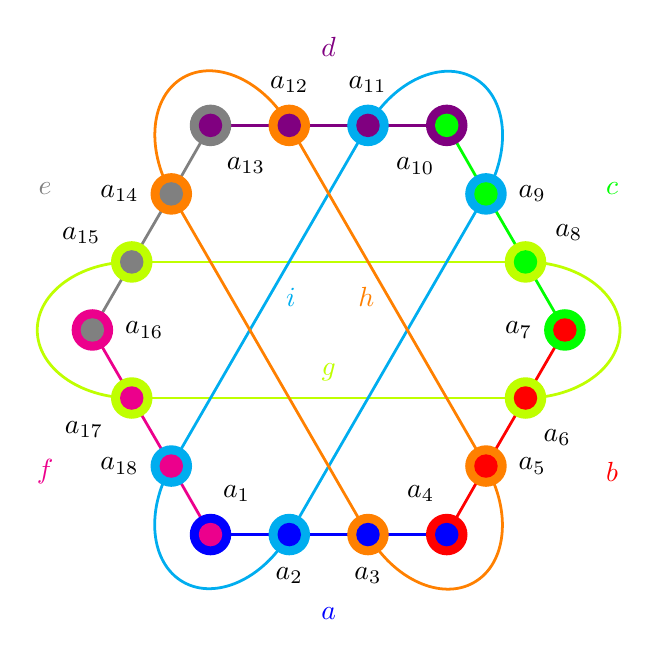
\begin{tikzpicture}  [scale=0.6]

        \tikzstyle{every path}=[line width=1pt]
        \tikzstyle{c2}=[circle,inner sep=3pt,minimum size=15pt]
        \tikzstyle{c1}=[circle,inner sep=3pt,minimum size=0pt]
        %\tikzstyle{s1}=[rectangle,minimum size=9]
        \tikzstyle{l1}=[draw=none,circle,minimum size=35]
        \tikzstyle{l2}=[draw=none,circle,minimum size=12]

        % Define positions of all observables
        \path
              (240:5) coordinate(1)
              (-0.833,-4.33) coordinate(2)
              (0.833,-4.33) coordinate(3)
              (300:5) coordinate(4)
              (3.33,-2.88) coordinate(5)
              (4.167,-1.44) coordinate(6)
     (0:5) coordinate(7)
              (4.167,1.44) coordinate(8)
              (3.33,2.88) coordinate(9)
              (60:5) coordinate(10)
              (0.833,4.33) coordinate(11)
              (-0.833,4.33) coordinate(12)
              (120:5) coordinate(13)
              (-3.33,2.88) coordinate(14)
              (-4.167,1.44) coordinate(15)
              (180:5) coordinate(16)
              (-4.167,-1.44) coordinate(17)
              (-3.33,-2.88) coordinate(18);

\node[draw=none,color=blue] at (0,-6) {$a$};
\node[draw=none,color=red] at (6,-3) {$b$};
\node[draw=none,color=green] at (6,3) {$c$};
\node[draw=none,color=violet] at (0,6) {$d$};
\node[draw=none,color=gray] at (-6,3) {$e$};
\node[draw=none,color=magenta] at (-6,-3) {$f$};
\node[draw=none,color=cyan] at (-0.8,0.7) {$i$};
\node[draw=none,color=orange] at (0.8,0.7) {$h$};
\node[draw=none,color=lime] at (0,-0.9) {$g$};



        % Draw all the context curves
        \draw [color=green] (7) -- (8) -- (9)-- (10);
\draw [color=violet] (10) -- (11) -- (12) -- (13);
\draw [color=gray] (13) -- (14) -- (15) -- (16);
\draw [color=magenta] (16) -- (17) -- (18) -- (1);
\draw [color=blue] (1) -- (2) -- (3) -- (4);
\draw [color=red] (4) -- (5) -- (6) -- (7);

        \draw [color=lime] (8) -- (15);
        \draw [color=lime](17) -- (6);
        \draw [color=lime] (8) arc (450:270:2 and 1.44);
        \draw [color=lime] (15) arc (90:270:2 and 1.44);

        \draw [color=cyan] (9) -- (2);
        \draw [color=cyan] (11) -- (18);
        \draw [rotate=240,color=cyan] (9) arc (90:270:2 and 1.44);
        \draw[rotate=60,color=cyan] (18) arc (90:270:2 and 1.44);

        \draw [color=orange] (12) -- (5);
        \draw [color=orange] (14) -- (3);
        \draw[rotate=300,color=orange] (12) arc (90:270:2 and 1.44);
        \draw[rotate=120,color=orange] (3) arc (90:270:2 and 1.44);

        % Draw the observables themselves
        \draw (1) coordinate[c2,fill=blue,label=85:$a_1$];
        \draw (1) coordinate[c1,fill=magenta];
        \draw (2) coordinate[c2,fill=cyan,label=270:$a_2$];
        \draw (2) coordinate[c1,fill=blue];
\draw (3) coordinate[c2,fill=orange,label=270:$a_3$];
        \draw (3) coordinate[c1,fill=blue];
        \draw (4) coordinate[c2,fill=red,label=95:$a_4$];
        \draw (4) coordinate[c1,fill=blue];
\draw (5) coordinate[c2,fill=orange,label=0:$a_5$];
        \draw (5) coordinate[c1,fill=red];
\draw (6) coordinate[c2,fill=lime,label=290:$a_6$];
        \draw (6) coordinate[c1,fill=red];
        \draw (7) coordinate[c2,fill=green,label=180:$a_7$];
        \draw (7) coordinate[c1,fill=red];
\draw (8) coordinate[c2,fill=lime,label=30:$a_8$];
        \draw (8) coordinate[c1,fill=green];
\draw (9) coordinate[c2,fill=cyan,label=0:$a_9$];
        \draw (9) coordinate[c1,fill=green];
        \draw (10) coordinate[c2,fill=violet,label=265:$a_{10}$];
        \draw (10) coordinate[c1,fill=green];
\draw (11) coordinate[c2,fill=cyan,label=91:$a_{11}$];
        \draw (11) coordinate[c1,fill=violet];
\draw (12) coordinate[c2,fill=orange,label=90:$a_{12}$];
        \draw (12) coordinate[c1,fill=violet];
        \draw (13) coordinate[c2,fill=gray,label=285:$a_{13}$];
        \draw (13) coordinate[c1,fill=violet];
\draw (14) coordinate[c2,fill=orange,label=180:$a_{14}$];
        \draw (14) coordinate[c1,fill=gray];
\draw (15) coordinate[c2,fill=lime,label=160:$a_{15}$];
        \draw (15) coordinate[c1,fill=gray];
        %%\draw (15) node[c1,fill=none] {\Huge $\times$};
        %\draw (15) coordinate[s1,fill,label=150:$P_c$];
        %\draw (15) coordinate[c1,fill=white];
        %%\draw (15) coordinate[c1,draw];
        \draw (16) coordinate[c2,fill=magenta,label=0:$a_{16}$];
        \draw (16) coordinate[c1,fill=gray];
\draw (17) coordinate[c2,fill=lime,label=215:$a_{17}$];
        \draw (17) coordinate[c1,fill=magenta];
\draw (18) coordinate[c2,fill=cyan,label=180:$a_{18}$];
        \draw (18) coordinate[c1,fill=magenta];

        % Context labels
        %\coordinate[l1,label=260:$C_1$] (c1) at (16);
        %\coordinate[l2,label=25:$C_2$] (c2) at (16);
    \end{tikzpicture}
\end{center}
\label{2018-m-ch-fdlvs-ksc}
\caption{Orthogonality diagram (hypergraph) of a configuration of observables without any two-valued state,
used in a parity proof of the Kochen-Specker theorem
presented in~\protect\bibentry{cabello-96}.}
\end{figure}





Note that, on the one hand,
each atom/point/vector/projector belongs
to exactly two -- that is, an {\em even} number of -- contexts; that is, it is biconnected.
Therefore,
%in order to obey non-contextuality -- in particular, the independence of any value of a two-valued state on the context it belongs to --
any enumeration of  all the contexts occurring in the graph
%depicted in Figure~\ref{2016-pu-book-chapter-qm-f-kspac}
would contain an {\em even} number of $1$s assigned.
Because due to noncontextuality and biconnectivity,
any atom $a$ with $v(a)=1$ along one context must have the same value 1 along the second context
which is intertwined with the first one -- to the values 1 appear in pairs.

Alas, on the other hand, in such an enumeration
there are nine  -- that is, an {\em odd} number of -- contexts.
Hence,
in order to obey the quantum predictions,
any  two-valued state (interpretable as truth assignment)
would need to have an {\em odd} number of $1$s -- exactly one for each context.
Therefore, there cannot exist any two-valued state on Kochen-Specker type graphs with the  ``parity property.''
%https://arxiv.org/pdf/1702.05215.pdf

More concretely,  note that, within each one of those 9 contexts,
the sum of any state on the atoms of that context must add up to 1.
That is, %due to additivity (\ref{2017-ch-pu-qlff}) and (\ref{2017-ch-pu-glff})
one obtains a system of 9 equations
\begin{equation}
\begin{split}
\color{blue}        v(a)= v( a_1 ) + v( a_2 ) + v( a_3 ) + v( a_4 ) = 1 ,                  \\
\color{red}         v(b)= v( a_4 ) + v( a_5 ) + v( a_6 ) + v( a_7 ) = 1 ,                  \\
\color{green}       v(c)= v( a_7 ) + v( a_8 ) + v( a_9 ) + v( a_{10} ) = 1 ,               \\
\color{violet}      v(d)= v( a_{10} ) + v( a_{11} ) + v( a_{12} ) + v( a_{13} ) = 1 ,      \\
\color{gray}        v(e)= v( a_{13} ) + v( a_{14} ) + v( a_{15} ) + v( a_{16} ) = 1 ,      \\
\color{magenta}     v(f)= v( a_{16} ) + v( a_{17} ) + v( a_{18} ) + v( a_1 ) = 1 ,         \\
\color{lime}        v(g)= v( a_6 ) + v( a_8 ) + v( a_{15} ) + v( a_{17} ) = 1 ,            \\
\color{orange}      v(h)= v( a_3 ) + v( a_5 ) + v( a_{12} ) + v( a_{14} ) = 1 ,            \\
\color{cyan}        v(i)= v( a_2 ) + v( a_9 ) + v( a_{11} ) + v( a_{18} ) = 1 .
\label{2017-b-e-cabp-conf}
\end{split}
\end{equation}
By summing up the left hand side and the right hand sides of the equations, and since all atoms are biconnected,
one obtains
\begin{equation}
2 \left[\sum_{i=1}^{18} v(a_i)\right] = 9.
\label{2017-b-e-cabp}
\end{equation}
Because $v(a_i)\in \{0,1\}$ the sum in (\ref{2017-b-e-cabp}) must add up to some natural number $M$.
Therefore, Equation~(\ref{2017-b-e-cabp}) is impossible to solve in the domain of natural numbers,
as on the left and right-hand sides, there appear even ($2M$) and odd ($9$) numbers, respectively.

Of course, one could also prove the nonexistence of any  two-valued state (interpretable as truth assignment)
by exhaustive attempts
(possibly exploiting symmetries) to assign values $0$s and $1$s to the atoms/points/vectors/projectors occurring in the graph
in such a way that both the quantum predictions as well as context independence are satisfied.
This latter method needs to be applied in cases with Kochen-Specker type diagrams (hypergraphs) without the  ``parity property;''
such as in the original Kochen-Specker proof.\cite[-50mm]{kochen1}


\bproof
}

Note also that in this original paper Kochen and Specker pointed out (in Theorem~0 on page~67)
that a much smaller set of quantum propositions  in intertwining contexts (orthonormal basis) suffices
to prove nonclassicality: all it needs is a configuration with a {\em nonseparating set}
of two-valued states; that is, there exist at least two observables with the same truth assignments for all
such truth assignments -- pointedly stated, the classical truth assignments
are unable to separate between those two observables.

Any such construction is usually based on a succession of  auxiliary  {\em gadget graphs}\cite[-0mm]{tutte_1954,SZABO2009436,Ramanathan-18}
\index{gadget graph}
stitched together to yield the desired property.
Thereby, gadgets are formed from gadgets of ever-increasing size and functional performance
(see also Chapter~12 of Ref.\cite[-0mm]{svozil-2016-pu-book}):
\begin{enumerate}

\item 0th order gadget:  a single context (aka clique/block/Boolean (sub)algebra/maximal observable/orthonormal basis);

\item 1st order ``firefly'' gadget:] two contexts connected in a single intertwining atom;

\item 2nd order gadget:  two 1st order  firefly  gadgets connected in a single intertwining atom;

\item 3rd order house/pentagon/pentagram gadget:  one firefly and one 2nd order gadget connected in two intertwining atoms to form a cyclic orthogonality diagram (hypergraph);

\item 4rth order true-implies-false (TIFS)/01-(maybe better 10)-gadget:  e.g., a Specker bug consisting of two pentagon gadgets connected by an entire context;
as well as extensions thereof to arbitrary angles for terminal (``extreme'') points;

\item 5th order  true-implies-true (TITS)/11-gadget:  e.g.,  Kochen and Specker's $\Gamma_1$, consisting of one 10-gadget and one firefly gadget,
connected at the respective terminal points;

\item 6th order gadget:  e.g.,  Kochen and Specker's $\Gamma_3$,
consisting of a combo of two 11-gadgets, connected  by their common firefly gadgets;

\item 7th order construction:  consisting of one 10- and one 11-gadget, with identical terminal points serving as constructions of Pitowsky's
principle of indeterminacy;~\cite{pitowsky:218,2015-AnalyticKS,svozil-2018-whycontexts}

\item 8th order construction:  concatenation of (10- and) 11-gadgets pasted/stitched together to form a graph used for proofs of the Kochen-Specker theorem;
e.g.,  Kochen and Specker's $\Gamma_2$.
\end{enumerate}


%%%%%%%%%%%%%%%%%%%%%%%%%%%%%%%%%%%%%%%%%%%%%%%%%%%%%%%%%%%%%%%%%%%%%%%%%%%%%%%%%%%%%%



\begin{center}
{\color{olive}   \Huge
%\decofourright
 %\decofourright \decofourleft
%\aldine X \decoone c
%\floweroneright
% \aldineleft ] \decosix g \leafleft
% \aldineright Y \decothreeleft f \leafNE
% \aldinesmall Z \decothreeright h \leafright
% \decofourleft a \decotwo d \starredbullet
%\decofourright
 \floweroneleft
}
\end{center}
